% =============================================================================
% Titel:	Experimentalphysik IV - Mitschrieb
% Erstellt:	SS 09
% Dozent:	Prof. Dr. Tilman Pfau
% Autor:	Jan-Cornelius Molnar
% =============================================================================
\documentclass[paper=a5,fleqn,DIV=calc]{scrartcl}

% =============================================================================
% 					Benötigte Pakete
% =============================================================================
\usepackage{janmcommon}
\usepackage{janmscript}
\usepackage{listings}
\usepackage{float}
\restylefloat{figure}
\usepackage[innercaption]{sidecap}

% =============================================================================
% 					Ana-Theorem-Style
% =============================================================================
% Theorem Umgebungen *MIT* Numerierung
\theoremstyle{graymarginwithblueheader}
\theorembodyfont{\itshape}
\theoremseparator{}
\theoremsymbol{}

\newtheorem{prop}{Satz}[section]
\newtheorem{lem}[prop]{Lemma}
\newtheorem{defn}[prop]{Definition}
\newtheorem{cor}[prop]{Korollar}

\theoremstyle{graymarginwithyellowheader}
\theorembodyfont{\normalfont}
\theoremseparator{}
\theoremsymbol{}

\newtheorem{bsp}[prop]{Bsp}

\theoremstyle{graymarginwithitblackheader}
\theorembodyfont{\normalfont}
\theoremseparator{}
\theoremsymbol{}

\newtheorem{bem}[prop]{Bemerkung.}

% Theorem Umgebungen *OHNE* Numerierung
\theoremstyle{graymarginwithblueheadern}
\theorembodyfont{\itshape}
\theoremseparator{}
\theoremsymbol{}

\newtheorem{propn}{Satz}
\newtheorem{lemn}{Lemma}
\newtheorem{corn}{Korollar}
\newtheorem{defnn}{Definition}

\theoremstyle{graymarginwithyellowheadern}
\theorembodyfont{\normalfont}
\theoremseparator{}
\theoremsymbol{}

\newtheorem{bspn}{Bsp}

\theoremstyle{graymarginwithitblackheadern}
\theorembodyfont{\normalfont}
\theoremseparator{}
\theoremsymbol{}

\newtheorem{bemn}{Bemerkung.}
%\renewcommand{\vec}[1]{\textbf{#1}}

% =============================================================================
% 					Ana-Überschriften-Style
% =============================================================================
\renewcommand\thesection{\arabic{section}}
\renewcommand\thesubsection{\arabic{section}-\arabic{subsection}}
\renewcommand\thesubsubsection{\small\ensuremath{\blacksquare}\normalsize}

\titleformat{\section}%
  {\normalfont\bfseries\Huge\color{darkblue}}%
  {\thesection}%
  {0.6em}%
  {}%
  
\titleformat{\subsection}%
  {\normalfont\bfseries\Large\color{darkblue}}%
  {\thesubsection}%
  {0.6em}%
  {}%

\titleformat{\subsubsection}%
  {\normalfont\bfseries\color{darkblue}}%
  {\thesubsubsection}%
  {0.2em}%
  {}%

\renewcommand{\labelenumi}{{\normalfont(\alph{enumi})}}

\newcommand{\kin}{\text{\tiny kin}}

\newcommand{\oline}[1]{\ensuremath{\overline{\text{#1}}}}

\newcommand{\op}[1]{\hat{\boldmath{#1}}}

\psset{linecolor=gdarkgray}
\psset{tickcolor=gdarkgray}
\psset{fillcolor=glightgray}

\newcommand{\scaption}[2]{%
	\caption[#1]{#1}%
	\footnotetext{#2}%
}

\newcommand{\BethgeSchroeder}%
	{\textit{K. Bethge, U. E. Schröder}, %
	Elementarteilchen und ihre Wechselwirkungen}
	
\newcommand{\BethgeWalter}%
	{\textit{K. Bethge, G. Walter, B. Wiedemann}, %
	Kernphysik – Eine Einführung}
	
\newcommand{\DemtroederThree}
	{\textit{W. Demtröder}, %
	Experimentalphysik 3}
	
\newcommand{\DemtroederFour}
	{\textit{W. Demtröder}, %
	Experimentalphysik 4}

\newcommand{\FrauenfelderHenley}%
	{\textit{H. Frauenfelder, E. M. Henley}, %
	Teilchen und Kerne: Die Welt der subatomaren Physik}

\newcommand{\KuckukKern}%
	{\textit{T. Mayer-Kuckuk}, %
	Kernphysik}
	
\newcommand{\KuckukAtom}%
	{\textit{T. Mayer-Kuckuk}, %
	Atomphysik}
	
\newcommand{\HakenWolf}%
	{\textit{H. Haken, H. C. Wolf}, %
	Atom-und Quantenphysik}
	
\newcommand{\HertelSchulz}%
	{\textit{I. Hertel, C. P. Schulz}, %
	Atome, Moleküle und optische Physik 1}
	
\newcommand{\Stierstadt}% 
	{\textit{K. Stierstadt}, %
	Physik der Materie}
	
\newcommand{\TiplerMPFife}%
	{\textit{P. A. Tipler, R. A. Llewellyn}, %
	Modern Physics, Fifth Edition}
	
\newcommand{\erstesargument}{}
\newcommand{\zweitesargument}{}

\newcommand{\qfigure}[4]{%
% 1 - breite der Minipage
% 2 - breite der Grafik (in der Minipage)
% 3 - pfad zur Grafik
% 4 - fußnote
\begin{minipage}{#1\linewidth}%
	\renewcommand{\footnoterule}{}%
	\centering%
	\includegraphics[width=#2\textwidth]{fig/#3}%
	\footnotetext{#4}
\end{minipage}%
}

\usepackage{twoopt}

\newcommandtwoopt{\sfigure}[5][!htpb][0.8]{%
 \begin{figure}[#1]%
  \centering
  \qfigure{1}{#2}{#3}{#4}
  \caption{#5}
 \end{figure}%
}

\newcommandtwoopt{\rfigure}[5][!htpb][0.6]{%
 \begin{SCfigure}[5][#1]%
  \centering%
  \includegraphics[width=#2\textwidth]{fig/#3}%
  \caption{#5\\\color{black}\normalfont\footnotesize\textrm{#4}}%
 \end{SCfigure}%
}

\newcommand{\twofigures}[1][!htbp]{% erstes optionales Argument
\begingroup  % Definitionen von \...argument lokal halten
	\renewcommand{\erstesargument}{#1}% opt. Argument speichern
	\twofiguresZwei}
  \newcommand{\twofiguresZwei}[1][0.5]{% zweites optionales Argument
      \renewcommand{\zweitesargument}{#1}% opt. Argument speichern
      \twofiguresDrei}
  \newcommand{\twofiguresDrei}[6][0.5]{% drittes opt. + notwendiges Argument
   \begin{figure}[\erstesargument]%
   \centering
	\qfigure{\zweitesargument}{1}{#2}{#3}
	\qfigure{#1}{1}{#4}{#5}
	\caption{#6}
	\end{figure}%
\endgroup}

% =============================================================================
% 					Document-Body
% =============================================================================
\begin{document}

% Titel
\begin{center}
{\huge\bf Exphys IV - Mitschrieb}

bei Prof. Dr. T. Pfau

Jan-Cornelius Molnar, Version: \today\ \thistime
\end{center}

% Inhaltsverzeichnis
\tableofcontents

% Inhalt
\newpage
\section{Symmetrien in der Physik}

\subsection{Aufbau der Materie}

In dieser Vorlesung werden wir uns mit den elementaren Bausteinen der Materie
und ihren Wechselwirkungen befassen. Dadurch soll ein quantifizierbarer und
nachvollziehbarer Zugang zur Wirklichkeit gefunden werden. Zunächst sollten wir
jedoch die Frage klären, was ``elementar'' überhaupt bedeutet. In der
Vergangenheit wurden zunächst die Atome für unteilbar gehalten, dann entdeckte
man Elektronen, Neutronen, Protonen und heute sprechen wir von ``Quarks'' als
Elementarteilchen. Im Folgenden werden wir uns mit diesem Postulat kritisch
auseinandersetzen.
\begin{figure}[!ht]
  \centering
\begin{pspicture}(-0.2,-4.4)(7.5,1.25)

\rput(1.5,0.7){Elementarteilchen}
\rput(5.2,0.7){Wechselwirkungen}

\psellipse[linewidth=0.04,dimen=outer](1.5,0.7)(1.5,0.5)
\psellipse[linewidth=0.04,dimen=outer](5.2,0.7)(1.5,0.5)

\rput(3.2,-0.17){Hadronen}
\psline{->}(3.2,-0.47)(3.2,-0.87)

\rput(3.2,-1.17){Kerne}
\psline{->}(3.2,-1.47)(3.2,-1.87)

\rput(3.2,-2.17){Atome}
\psline{->}(3.2,-2.47)(3.2,-2.87)

\rput(3.2,-3.17){Moleküle}
\psline{->}(3.2,-3.47)(3.2,-3.87)
\psline{->}(4.2,-3.47)(4.8,-3.87)
\psline{->}(2.2,-3.47)(1.6,-3.87)

\rput(3.2,-4.17){Flüssigkeit}
\rput(5.2,-4.17){Festkörper}
\rput(1.2,-4.17){Gas}

% Trennlinien
\psline(5.15,-1.6)(7.4,-1.6)
\psline(1.55,-2.8)(0.0,-2.8)

\psline{->}(5.2,0)(5.2,-1.4)
\psline{->}(1.5,0)(1.5,-2.6)

\psline{->}(5.2,-1.8)(5.2,-3.87)

\rput[l](5.4,-0.8){Starke und}
\rput[l](5.4,-1.2){Schwache WW}
\rput[l](5.4,-2.6){EM WW}
\rput{-90}(0.6,-0.4){\rput(0.9,0.4){Diese Vorlesung}}
\end{pspicture} 
  \caption{Übersicht Elementarteilchen, Wechselwirkungen.}
\end{figure}

Primär werden wir es mit der starken, schwachen sowie der elektromagnetischen
Wechselwirkung zu tun haben. Die Gravitation wird in dieser Vorlesung nur eine
untergeordnete Rolle spielen und kann so lange wir Elementarteilchen
betrachten vernachlässigt werden.

\sfigure[H]%
	{1-EigenschaftenDerWechselwirkungen.pdf}
	{\BethgeSchroeder, S. 10}
	{Charakteristische Eigenschaften der Wechselwirkungen.}
	
\sfigure[H]%
	{1-Langenskalen.pdf}
	{\FrauenfelderHenley, S. 2}
	{Typische Längenskalen. Der Bereich unterhalb von $10^{-18}\mathrm{m}$ ist 
		unerforscht! Es ist nicht bekannt, ob dort neue Kräfte und Erscheinungen zu
		erwarten sind.}%
	
\sfigure[H]%
	{1-Anregungsenergien.pdf}
	{\FrauenfelderHenley, S. 2}
	{Bereich der Anregungsenergien. Die angegebenen Temperaturen entsprechen den
	jeweiligen Energien.}%
	
\sfigure[H]%
	{1-Dichtebereiche.pdf}
	{\FrauenfelderHenley, S. 2}
	{Dichtebereiche.}%
	
\subsubsection{Symmetriebrechung}

Es sei eine Temperaturskala mit Phasenübergang bei einer kritischen Temperatur
$T_C$ gegeben. In der Thermodynamik verwenden wir die \emph{freie Energie} $F$,
um den Zustand eines Systems zu beschreiben, wobei die freie Energie von einem
Ordnungsparameter $\ph$ abhängt.

Generell erhält man für hohe Temperaturen bzw. Energien eine höhere Symmetrie
welche bei niedrigeren Temperaturen gebrochen wird.
\begin{figure}[!ht]
  \centering
\begin{pspicture}(-1,-1)(4.5,2.5)
 \psaxes[labels=none,ticks=none]{->}%
 (0,0)(-0.5,-0.5)(4,2)[,-90][\color{gdarkgray}$T$,0]
 
 \psyTick(1){\color{gdarkgray}T_C}
 
 \rput[l](0.5,1.5){Hohe Symmetrie}
 
 \rput[l](0.5,0.5){Niedere Symmetrie}
\end{pspicture}
  \caption{Symmetriebrechung durch Temperaturänderung.}
\end{figure}

\begin{bspn}
\begin{figure}[!ht]
  \centering
\begin{pspicture}(-2.5,-1)(2.5,2.5)
 \psaxes[labels=none,ticks=none]{->}%
 (0,0)(-2,-0.5)(2,2)[\color{gdarkgray}$\ph$,-90][\color{gdarkgray}$F$,0]

 \pscircle[linewidth=0.6pt](0,0.2){0.2}
 
 \psplot[linewidth=1.2pt,%
	     linecolor=darkblue,%
	     algebraic=true]%
	     {-1.5}{1.5}{0.6*x^2}
 
 \rput[l](1.2,0.4){\color{gdarkgray}$T>T_c$}
 
 \rput(0,-0.8){\color{gdarkgray}Symmetrie}
\end{pspicture}
\begin{pspicture}(-2.5,-1.6)(2.5,2.5)
 \psaxes[labels=none,ticks=none]{->}%
 (0,0)(-2,-0.5)(2,2)[\color{gdarkgray}$\ph$,-90][\color{gdarkgray}$F$,0]
 
 \pscircle[linewidth=0.6pt](0.85,-0.35){0.2}
 
 \psplot[linewidth=1.2pt,%
	     linecolor=darkblue,%
	     algebraic=true]%
	     {-1.5}{1.5}{x^4-1.5*x^2}
 
 \rput[l](0.2,1.4){\color{gdarkgray}$T<T_c$}
 
 \psbezier[arrows=<->](-0.85,-0.6)(-0.55,-1.2)(0.55,-1.2)(0.85,-0.6)
 \rput(0,-1.4){\color{gdarkgray}Symmetriebrechnung}
\end{pspicture}
  \caption{Symmetriebrechung in der Thermodynamik.}
\end{figure}

Wir kennen dieses Verhalten bereits von Ferromagneten. Hier wird die Ordnung
durch den Ordnungsparameter Magnetisierung ($\ph=M$) beschrieben. Wird eine
kritische Temperatur überschritten (\emph{Curie-Temperatur}), so haben die
elementaren Dipole keine Vorzugsrichtung mehr und der Magnet wird zum
Paramagneten.
\begin{figure}[!ht]
  \centering
\begin{pspicture}(-1,-2)(4,2.5)
 \psaxes[labels=none,ticks=none]{->}%
 (0,0)(-0.5,-2)(3.5,2)[\color{gdarkgray}$H$,-90][\color{gdarkgray}$T$,0]

 \psplot[linewidth=1.2pt,%
	     linecolor=darkblue,%
	     algebraic=true]%
	     {0}{1.15}{x^4}
 
 \psplot[linewidth=1.2pt,%
	     linecolor=darkblue,%
	     algebraic=true]%
	     {0}{1.15}{-x^4}
 
  \rput[bl](0.2,1.2){\color{gdarkgray}para}
 \rput[bl](0.2,-1.2){\color{gdarkgray}ferro}
\end{pspicture}
\begin{pspicture}(-1,-1)(4,2.5)
 \psaxes[labels=none,ticks=none]{->}%
 (0,0)(-0.5,-0.5)(3.5,2)[\color{gdarkgray}$T$,-90][\color{gdarkgray}$M$,0]
 
 \psarc[linewidth=1.2pt,%
	    linecolor=darkblue]%
	   (0.5,0){2}{0}{87}
	   
 \psxTick(2.5){\color{gdarkgray}T_c}
 
 \rput[lb](1.5,0.25){\color{gdarkgray}ferro}
 \rput[lb](2.7,0.25){\color{gdarkgray}para}
\end{pspicture}
  \caption{Verhalten eines Ferromagneten bei Curie-Temperatur.}
\end{figure}

Bei dieser Temperatur liegt eine höhere Symmetrie vor, denn der Magnetismus ist
isotrop also Richtungsunabhängig. Kühlt man den Magneten ab, ordnen sich die
Dipole wieder entlang ihrer Vorzugsrichtung starr an, die räumliche Symmetrie
innerhalb der ferromagnetischen Domäne geht verloren. Diesen Vorgang nennt man
spontane Symmetriebrechung.

Betrachten wir die Welt um uns herum, so finden wir zahlreiche gebrochene
Symmetrien, die bei hohen Energien bzw. Temperaturen wiederhergestellt werden.
Kristalle schmelzen; gebundene Zustände werden in ihre Bestandteile zerlegt wie
z.B. Gase gehen in Plasmen über etc.

Um die elementaren Bestandteile der Materie zu finden, ist es daher hilfreich,
die Energie immer weiter zu erhöhen und die verbleibenden Symmetrien zu
skechieren.
\bsphere
\end{bspn}

Zur Beschreibung der Gravitation verfügen wir über die Einsteinschen
Feldgleichungen und die Allgemeine Relativitätstheorie, für den
Elektromagnetismus über die Maxwell Gleichungen. In beiden Fällen
sind die Gleichungen lorentzinvariant, d.h. Lorentztransformationen sind
elementare Symmetrieoperationen. 
Für die starke und schwache Wechselwirkung sind (noch) keine Grundgleichungen
verfügbar, man ist daher auf der Suche nach zusätzlichen Symmetrien.
 
Das Konzept der Symmetrie spielt eine wichtige Rolle bei hohen Energien, da
dort neue Symmetrien auftreten. Man vermutet, dass sich bei sehr hohen Energien
die starke, schwache und elektromagnetische Wechselwirkung und die Gravitation
zu einer einzigen Wechselwirkung mit einer neuen Symmetrie vereinen. Diese
Symmetrie wird im Niederenergiebereich gebrochen und führt zu den
unterschiedlichen Wechselwirkungen, die wir mit niederer Symmetrie heute
beobachten.
\twofigures[!htbp][0.4][0.5]%
	{1-VergleichGesamtwirkungsquerschnitte.pdf}%
	{\FrauenfelderHenley, S. 428}%
	{1-EnergienVergleich.pdf}%
	{P. A. Tipler, R. A. Llewellyn, Modern Physics, Fifth Edition S. 605}
	{Vergleich der Gesamtwirkungsquerschnitte von hadronischen, elektromagnetischen
	und schwachen Prozessen an Nukleonen. $\sigma$ bezeichnet den geometrischen
	Wirkungsquerschnitt eines Nukleons, $K$ gibt die kinetische Energie an.}%

Die vermutetete Symmetrie kann helfen, die Zustände zu
erklären, die bei der Entstehung des Universums vorzufinden waren. Denn zu
jeder neuen Symmetrie gehört auch ein neuer Erhaltungssatz. Aber auch das
Verhalten komplexer Kernmaterie zeigt Phasenübergänge und Symmetriebrechung. 

\sfigure[H][0.8]%
	{1-PhasendiagrammKerne.pdf}%
	{\FrauenfelderHenley, S. 514}%
	{Phasendiagramm für Kerne.}


\begin{bspn}
Betrachten wir die Temperaturkurve von Kernmaterie in Abhängigkeit der
Anregungsenergie pro Nukleon, so ergibt sich eine große Ähnlichkeit zum Verlauf der Temperaturkurve von
Wasser in Abhängigkeit der Anregungsenergie pro Molekül. Solche Analogien
helfen und dabei, das Verhalten der Kerne auf bekanntes zu übertragen und so
ein Modell für die Kerne zu entwickeln.\bsphere
\end{bspn}

\sfigure[H]%
	{1-TemperaturdiagrammKernmatWasser.pdf}%
	{\BethgeWalter, S. 216}%
	{Temperaturdiagramm für (a) Kernmaterie und (b) Wasser.}

\subsection{Symmetrien und Erhaltungssätze (klassisch)}

In diesem Abschnitt sollen Symmetrien mathematisch formuliert werden. Durch
diesen Formalismus lässt sich aus jeder Symmetrie ein Erhaltungssatz ableiten.

Unter einer Symmetrie versteht man eine Operation $\op{S}$, die ein
physikalisches Objekt oder Gesetzt $O$ invariant lässt,
\begin{align*}
\op{S}(O) = O.
\end{align*}
$O$ nennt man auch \emph{Observable}.

\begin{bspn}
\emph{Paritätssymmetrie}. 
Wir beobachten ein Phänomen bspw. eine Teilchenbewegung sowohl gewöhnlich als
auch durch einen Spiegel. Eine Symmetrie liegt genau dann vor, wenn sich die
Physik im Spiegelbild nicht ändert.\bsphere
\end{bspn}
\begin{bspn}
\emph{Translationssymmetrie}.
Wechseln zwei Teilchen in einem abgeschlossenen homogenen System miteinander,
so ist die Wechselwirkung vom Koordinatenursprung unabhängig.
\begin{figure}[!ht]
  \centering
\begin{pspicture}(-0.1,-1.79)(5.6,1.77)
\pscircle[linewidth=0.04,dimen=outer](0.3,0.24){0.32}
\pscircle[linewidth=0.04,dimen=outer](5.2,1.38){0.32}

\psline(0.7928483,0.4704805)(1.3136523,0.21520971)(1.695397,0.7339302)(2.2282233,0.44050884)(2.5597954,0.9853575)(3.0855687,0.64777446)(3.4432688,1.2427961)(3.9439557,0.9182771)(4.2624636,1.4380393)(4.674827,1.1276263)
\psline(3.5,-1.7)(0.74,-0.09)
\psline(3.5,-1.7)(5.16,0.87)
\psdots(3.5,-1.7)

\rput(0.3,0.24){\color{gdarkgray}1}
\rput(5.2,1.38){\color{gdarkgray}2}

\rput(4.9,-0.2){\color{gdarkgray}$\vec{x}_1$}
\rput(2,-1.25){\color{gdarkgray}$\vec{x}_2$}
\rput(2.4,1.4){\color{gdarkgray}$V(\abs{\vec{x}_1-\vec{x}_2})$}
\end{pspicture} 
  \caption{2-Teilchen-Translationsinvarianz.}
\end{figure}

Eine Symmetrieoperation ist daher gegeben durch,
\begin{align*}
\hat{S}: \vec{x}_i \mapsto \vec{x}_i + \vec{a},
\end{align*}
wobei $\vec{a}$ für einen beliebigen Koordinatenursprung steht.
$\op{S}$ verändert als Symmetrieoperation die Wechselwirkung $V$
zwischen den Teilchen nicht, d.h. $\hat{S}(V) = V$. Aufgrund dieser Symmetrie erhalten
wir sofort die \emph{Impulserhaltung}.
\begin{align*}
\vec{p} = \vec{p}_1+\vec{p}_2,
\end{align*}
denn es gilt
\begin{align*}
\frac{\diffd}{\dt}\vec{p} = -\nabla V = -(\nabla_1+\nabla_2)V = -\nabla_1V -
\nabla_2V = 0.\Rightarrow \vec{p}=\const.\bsphere
\end{align*}
\end{bspn}
Um das letzte Beispiel zu verallgemeinern, führen wir die
\emph{Hamiltonfunktion}
\begin{align*}
H(p_i,q_i),
\end{align*}
ein mit den generalisierten Koordinaten $q_i$ und den kanonischen Impulsen
$p_i$. Eine Translation hat nun die Form,
\begin{align*}
\hat{S}: q_i \mapsto q_i + \delta q_i.
\end{align*}
Gilt $\hat{S}(H) = H$, so ist $\hat{S}$ eine Symmetrieoperation, d.h. $\hat{S}$
verändert die Hamiltonfunktion nicht. In diesem Fall gilt
\begin{align*}
&0 = \delta H = \delta q\sum_i \frac{\partial H}{\partial q_i} = -\delta q\sum_i
\dot{p}_i.\\
\Rightarrow & \frac{\diffd}{\dt} \sum_i \dot{p}_i = 0.
\end{align*}
Wir erhalten somit aus der Translationssymmetrie den Impulserhaltungssatz.

Ananlog erhält man aus der Rotationssymmetrie den Drehimpulserhaltungssatz und
aus der zeitlichen Translationssymmetrie die Energieerhaltung.

\subsection{Symmetrien in der Quantenmechanik}
Wir wollen die in der klassischen Mechanik entwickelte Theorie nun auf die
Quantenmechanik erweitern.
\begin{enumerate}[label=\arabic{*}.)]
\item Die verallgemeinerten Impulse und Koordinaten werden durch Operatoren
  ersetzt, die einer Vertauschungsrelation genügen.
  \begin{align*}
  \nrm{\hat{p}_i,\hat{q}_k} = i\hbar\delta_{ik}.
  \end{align*}
\item Die zu messenden Größen werden durch Erwartungswerte ersetzt,
\begin{align*}
\lin{\hat{\Omega}} = \int \dV \Psi^* \hat{\Omega}\Psi.
\end{align*}
\end{enumerate}
Ist $\hat{\Omega}$ eine Erhaltungsgröße, verschwindet die zeitliche Ableitung.
Es gilt 
\begin{align*}
i\hbar \frac{\diffd}{\dt}\lin{\hat{\Omega}}
&= \int\dV i\hbar \frac{\diffd}{\dt}\left[\Psi^*\hat{\Omega}\Psi\right]
\\&= \int \dV \left[\left(-\Psi^*i\hbar\frac{\diffd}{\dt}\right)\hat{\Omega}\Psi
 + \Psi^*\hat{\Omega}\left(i\hbar\frac{\diffd}{\dt}\Psi\right)\right]
\\ &= \int\dV -(\Psi^*\hat{H})\hat{\Omega}\Psi + \Psi^*\hat{\Omega}H\Psi
\\ &= \int\dV \Psi^*\left(\hat{\Omega}\hat{H} - \hat{H}\Omega\right)\Psi
\\ &= \lin{\nrm{\hat{H},\hat{\Omega}}}. 
\end{align*}
$\op{\Omega}$ ist also genau dann eine Erhaltungsgröße wenn $\op{H}$ und
$\op{\Omega}$ vertauschen.
\begin{bspn}
Drehung um die $z$-Achse.
\begin{align*}
\hat{S}:\; & x\mapsto x\cos\ph - y\sin\ph,\\
& y\mapsto x\sin\ph + y\cos\ph,\\
&z\mapsto z.
\end{align*}
\begin{figure}[H]
\centering
\begin{pspicture}(0,-1.35)(1.4178126,1.35)
\psline{->}(0.21,-0.50453126)(0.24,1.0649999)
\psline{->}(0.21,-0.50453126)(1.06,0.025)
\psline{->}(0.21,-0.50453126)(1.0,-1.0550001)

\rput(1.2878126,0.235){$y$}

\rput(1.1654688,-1.205){$x$}

\rput(0.2334375,1.255){$z$}
\psellipse[linecolor=darkblue](0.23,0.56000006)(0.23,0.17)
\psline[linecolor=darkblue]{->}(0.38,0.45000005)(0.46,0.51000005)
\end{pspicture} 
\caption{Drehung um die $z$-Achse.}
\end{figure}
Für eine Drehung um $\delta \ph$ gilt daher,
\begin{align*}
&\delta x = - y\delta\ph,\\
&\delta y = x\delta\ph,\\
&\delta z = 0,\\
\Rightarrow&\hat{S}\Psi(\vec{x}) = \Psi(\vec{x}) - \delta x
\frac{\partial\Psi}{\partial x} + \delta y \frac{\partial\Psi}{\partial y}
= \left(1-\delta\ph\left(x\frac{\partial}{\partial y}-y\frac{\partial}{\partial
x} \right) \right)\Psi(\vec{x}).
\end{align*}
Die Drehung hängt also mit der $z$-Koordinate des Drehimpulses
zusammen,
\begin{align*}
\hat{l}_z = \nrm{\hat{x}\times\hat{p}}_z = -i\hbar
\left(x\frac{\partial}{\partial y} - y\frac{\partial}{\partial x}\right).
\end{align*}
Die Drehung um die $z$-Achse können wir damit schreiben als,
\begin{align*}
\op{S}\Psi(\vec{x}) = \left(1- \frac{i}{\hbar}\partial\ph
\op{l}_z\right)\Psi(\vec{x}).
\end{align*}
Da wir infinitesimale Winkel $\delta\ph$ betrachten, können wir dies als
Taylor-Entwicklung 1. Ordnung des Exponential-Operators auffassen. Beim
Übergang zur kontinuierlichen Drehung erhält man,
\begin{align*}
\hat{S}:\;\Psi(\vec{x})\mapsto
\exp\left\{\frac{i}{\hbar}\ph\hat{l}_z\right\}\Psi(\vec{x}).
\end{align*}

Man bezeichnet $\hat{l}_z$ als \emph{Erzeugende} der Drehung um
die $z$-Achse. Betrachten wir nun den Hamilton Operator unter einer infinitesimalen
Drehung,
\begin{align*}
\hat{S}\left(\lin{\hat{H}}\right)
&= \int\dV \Psi^*\left(1-\frac{i}{\hbar}\delta\ph \op{l}_z\right)\hat{H}
\left(1+\frac{i}{\hbar}\delta\ph \op{l}_z\right)\Psi\\
&= \int\dV \Psi^*\hat{H}\Psi +
\Psi^*\hat{H}\left(\frac{i}{\hbar}\delta\ph \op{l}_z\right)\Psi
- \Psi^*\left(\frac{i}{\hbar}\delta\ph \op{l}_z\right)\hat{H}\Psi \\
&+\underbrace{\frac{1}{\hbar^2}\delta\ph^2\Psi^*\op{l}_z\hat{H}\op{l}_z\Psi}_{ 
= 0, \text{ da quadratisch in $\delta\ph$}.}\\
&= \int\dV \Psi^*\left[\hat{H} - \frac{i}{\hbar}\left(\op{l}_z\hat{H} -
\hat{H}\op{l}_z\right)\right]\Psi\\ &\overset{!}{=} \lin{\hat{H}},
\end{align*}
dann gilt die Gleichheit genau dann, wenn $\hat{l}_z$ mit dem Hamilton
vertauscht,
\begin{align*}
\nrm{\hat{l}_z,\hat{H}} = 0.
\end{align*}
Rotationssymmetrie um die $z$-Achse impliziert also wie in der klassischen
Mechanik die Erhaltung des Drehimpulses um die $z$-Achse.\bsphere
\end{bspn}

\subsection{Relativistische Invarianz}

Eine \emph{Lorenztransformation}\footnote{Hendrik Antoon Lorentz (* 18. Juli
1853 in Arnheim; † 4. Februar 1928 in Haarlem) war ein niederländischer
Mathematiker und Physiker und Nobelpreisträger für Physik des Jahres 1902.}, 
erhält den Abstand zweier Punkte in der Raumzeit. Eine Größe, die sich unter
einer Lorentztransformation nicht ändert, heißt \emph{lorentzinvariant}.

Die Lorenztransformation ist somit eine Symmetrieoperation $\hat{S}$ mit einer
Invarianten $s$, dem raumzeitlichen Abstand, gegeben durch,
\begin{align*}
s^2 = c^2(t_1-t_2)^2 - (x_1-x_2)^2 - (y_1-y_2)^2 - (z_1-z_2)^2 = \const.
\end{align*}
\begin{bspn}
Lineare Bewegung in $x$-Richtung mit Geschwindigkeit $v$,
\begin{align*}
\hat{S}:\; & ct' = c(\cosh \alpha)t - x(\sinh\alpha)\\
& x' = x\cosh \alpha - c(\sinh \alpha)t\\
& y' = y\\
& z' = z
\end{align*}
wobei
\begin{align*}
&\cosh \alpha = \frac{1}{\sqrt{1-\beta^2}},\quad
\sin\alpha = \frac{\beta}{\sqrt{1-\beta^2}},\quad
 \beta=\frac{v}{c}.
\end{align*}
Da $\sinh^2 \alpha - \cosh^2 \alpha = 1$ gilt $\hat{S}(s^2)=s^2$.\bsphere
\end{bspn}

Um in der Raumzeit geschickt rechnen zu können, führen wir verallgemeinerte
Vektoren ein, die \emph{Vierervektoren},
\begin{align*}
\vec{x}^\mu = \left\{ct,x,y,z \right\}.
\end{align*}
Für diese Vektoren definieren wir ein neues Skalarprodukt
\begin{align*}
\abs{\vec{x}}^2 = \lin{\vec{x}_\mu,\vec{x}^\mu} = \sum\limits_{\mu=0}^3
x_\mu x^\mu = c^2t^2 - x^2-y^2-z^2.
\end{align*}
Die Energie $E=\frac{mc^2}{\sqrt{1-\beta^2}}$ und der Impuls $\vec{p} =
\frac{m\vec{v}}{\sqrt{1-\beta^2}}$ bilden den Viererimpuls,
\begin{align*}
\vec{p}^\mu = \left\{ \frac{E}{c}, p_x, p_y, p_z\right\}.
\end{align*}
Durch obige Definition ist das Skalarprodukt invariant unter
Lorentztransformationen. Insbesondere gilt
\begin{align*}
\lin{\hat{S}p_\mu,\hat{S}p^\mu} = \lin{p_\mu,p^\mu} = \sum\limits_{\mu=0}^3
p_\mu p^\mu = \frac{E^2}{c^2} - p^2 = mc^2 = \const.\tag{*}
\end{align*}

Insbesondere erhalten wir für $p=0$ die Ruheenergie $E_0 = mc^2$.
Durch Lorentztransformationen kann somit Ruhemasse in kinetische Energie
umgewandelt werden und umgekehrt.
\begin{bspn}
Bei einem Stoßprozess sind $E_\tot$ und $\vec{p}_\tot$ erhalten, aber $m_\tot =
\sum_i m_i\neq \const$. Insbesondere kann kinetische Energie in Ruhemasse und
Ruhemasse in kinetische Energie umgewandelt werden.
\begin{figure}[!htpb]
  \centering
\begin{pspicture}(-0.1,-2)(3,2)
\psline{->}(0,1.5)(2,1.5)
\psline[linestyle=dotted]{->}(0,0)(2,0)
\psline{->}(0,-1.5)(2,-1.5)

\rput(2.5,1.5){\color{gdarkgray}$E_+$}
\rput(2.5,-1.5){\color{gdarkgray}$E_-$}
\rput(2.5,0){\color{gdarkgray}$0$}
\end{pspicture} 
  \caption{Energie-Masse-Äquivalenz.}
\end{figure}
\textit{Zahlenbeispiel:} $10^{-4}g\entspr 2500 \mathrm{kWh}$.

Aus (*) folgt,
\begin{align*}
E = \pm c\sqrt{p^2+m^2c^2}.
\end{align*}
Dass zwei Vorzeichen $\pm$ möglich sind, kündigt die Existenz von Antiteilchen
an. Beispielsweise kann für $E_\kin > 2m_ec^2$ bei einem Stoßprozess ein
$e^+,e^-$-Paar erzeugt werden.\bsphere
\end{bspn}

\subsection{Der Spin}
Zur Charakterisierung eines Teilchens benötigt man folgende Größen:

%\begin{table}
\begin{tabular}[H]{ll}
$m_\text{träge}$, $m_\text{schwer}$ & Gravitation\\
$Q$ & Elektromagnetismus\\
Farbladungen & Starke + Schwache WW\\
$\vec{p},\vec{L},E$ & Beschreiben Bewegung des Schwerpunkts\\
Spin & innerer Freiheitsgrad.
\end{tabular}
%\end{table}

Wir wollen nun der Frage nachgehen wie viele ``Sorten'' Spin es geben kann.
Klassisch wird der Spin eines Objekts oft mit dem Eigendrehimpuls
identifiziert. Bei Elementarteilchen mit
verschwindender Ausdehnung ($r\to0$) versagt jedoch die Vorstellung. Außerdem
würde eine klassisch rotierende Ladung ein anderes magnetisches Moment erzeugen
als das experimentell beobachtete (siehe $g$-Faktor des Elektonsr
$g=2.001\ldots$).

In der Quantenmechanik definiert man daher \emph{Spinoperatoren}, die den
selben Vertauschungsrelationen wie Drehimpulsoperatoren folgen.
\begin{align*}
&\nrm{\hat{s}_i,\hat{s}_j} = i\hbar\ep_{ijk} \hat{s}_k,\qquad
\ep_{123} =
\begin{cases}
1, & \text{zyklische Vertauschung von (1,2,3)},\\
-1, & \text{antizyklische Vertauschung},\\
0, & \text{sonst}.
\end{cases}
\end{align*}
\begin{bspn} Im dreidimensionalen Fall erhalten wir,
\begin{align*}
\nrm{\hat{s}_x,\hat{s}_y} = i\hbar \ep_{xyz}\hat{s}_z.\bsphere
\end{align*}
\end{bspn}
Das skalare Quadrat des Spins ist gegeben durch,
\begin{align*}
\hat{s}^2 = \underbrace{\hat{s}_x^2 + \hat{s}_y^2 + \hat{s}_z^2}_{\ge 0}.\tag{*}
\end{align*}
Die Eigenwerte von $\hat{s}$ werden mit $s$ die von $\hat{s}_z$ mit
$m_s$ bezeichnet. Man kann zeigen dass die gemeinsamen Eigenzustände
$\ket{s,m_s}$ von $\hat{s}$ und $\hat{s}_z$ ein VONS bilden. Da die Eigenwerte
von $\hat{s}^2$ positiv sind (siehe (*)), lassen sie sich als $s(s+1)$
schreiben, womit wir folgende Eigenwertgleichungen erhalten,
\begin{align*}
&\hat{s}^2\ket{s,m_s} = s(s+1)\hbar^2\ket{s,m_s},\\
&\hat{s}_z\ket{s,m_s} = m_s\hbar\ket{s,m_s}.
\end{align*}
\begin{bemn}
Da $\nrm{\hat{s}^2,\hat{s}_z}=0$, sind $\hat{s}^2$ und $\hat{s}_z$ zwei
gleichzeitig beobachtbare Erhaltungsgrößen.\maphere
\end{bemn}
Wir wollen nun mit Hilfe der Eigenwertgleichungen $s$ und $m_s$ konkret
berechnen. Dazu halten wir fest,
\begin{align*}
&\hat{s}^2\ket{s,m_s} = f(s,m_s)\ket{s,m_s},\\
&\hat{s}^2-\hat{s}_z^2 = \underbrace{\hat{s}_x^2 + \hat{s}_y^2}_{\ge 0}.
\end{align*}
Es gilt also $f(s,m_s)\ge \hbar^2 m_s^2$, d.h. $m_s$ hat einen Maximalwert.

Oft ist es geschickt anstatt mit $\hat{s}_x$, $\hat{s}_y$ oder $\hat{s}_z$ mit
einer der folgenden Linearkombinationen zu rechnen.
\begin{defnn}
\emph{Leiteroperatoren}
\begin{align*}
&\hat{s}_+ := \hat{s}_x + i\hat{s}_y,&& \text{``Aufsteigeoperator''},\\
&\hat{s}_- := \hat{s}_x - i\hat{s}_y,&& \text{``Absteigeoperator''}.
\end{align*}
Als Linearkombinationen von $\hat{s}_x$ und $\hat{s}_y$ erfüllen sie
die Vertauschungsrelationen,
\begin{align*}
&\nrm{\hat{s}^2,\hat{s}_\pm} = 0,&&\text{d.h. }\hat{s}_\pm\text{ ändert $s$
nicht}.\\ &\nrm{\hat{s}_z,\hat{s}_\pm} =\pm\hbar\hat{s}_\pm, &&\text{d.h.
$\hat{s}_\pm$ ändert $m_s$}.\fishhere
\end{align*}
\end{defnn}
Betrachten wir nun die zwei Zustände $\hat{s}_\pm\ket{s,m_s} $ und die Wirkung
von $\hat{s}_z$ und $\hat{s}^2$,
\begin{align*}
\hat{s}_z\hat{s}_\pm\ket{s,m_s} &= \left(\hat{s}_\pm\hat{s}_z +
\nrm{\hat{s}_z,\hat{s}_\pm}\right)\ket{s,m_s}
= \left(\hat{s}_\pm\hat{s}_z \pm
\hbar\hat{s}_\pm\right)\ket{s,m_s}
\\ &= \left( \hbar m_s\hat{s}_\pm \pm
\hbar\hat{s}_\pm\right)\ket{s,m_s}
= \hbar (m_s \pm 1)\hat{s}_\pm\ket{s,m_s},\\
\hat{s}^2\hat{s}_\pm\ket{s,m_s} &= \hat{s}_\pm\hat{s}^2\ket{s,m_s} =
\hbar^2 l(l+1)\hat{s}_\pm\ket{s,m_s}.
\end{align*}
Da $m_s$ einen Maximalwert besitzt, erhalten wir so:

$\hat{s}_+\ket{s,m_s}$ ist Eigenzustand zu $\hat{s}^2$ und $\hat{s}_z$ mit
den Eigenwerten $\hbar^2s(s+1)$ bzw. $\hbar (m_s+1)$ oder der Nullvektor.

$\hat{s}_-\ket{s,m_s}$ ist Eigenzustand zu $\hat{s}^2$ und $\hat{s}_z$ mit
den Eigenwerten $\hbar^2s(s+1)$ bzw. $\hbar (m_s-1)$ oder der Nullvektor.

Betrachten wir die Norm 
$\norm{\hat{s}_\pm\ket{s,m_s}}^2=\bra{s,m_s}\hat{s}_\mp\hat{s}_\pm\ket{s,m_s}$
und verwenden,
\begin{align*}
\hat{s}_\mp\hat{s}_\pm = (\hat{s}_x\mp i\hat{s}_y)(\hat{s}_x\pm i\hat{s}_y) =
\hat{s}_x^2+\hat{s}_y^2 \pm i\nrm{\hat{s}_x,\hat{s}_y} = \hat{s}^2 -
\hat{s}_z^2 \mp \hbar\hat{s}_z
\end{align*}
erhalten wir,
\begin{align*}
\norm{\hat{s}_\pm\ket{s,m_s}}^2 = \left[l(l+1) - m_s(m_s\pm1)\right]\hbar^2 \ge
0.\tag{**}
\end{align*}
D.h. $-s\le m_s \le s$.

Aufgrund der Einschränkung der möglichen $m_s$ muss $\hat{s}_+\ket{s,s}$ der
Nullvektor sein, denn $\hat{s}_+$ erhöht $m_s$. Daher ist
$\norm{\hat{s}_+\ket{s,s}}^2=0 \Rightarrow m_{s,\text{max}} = s$.

Analog folgt $m_{s,\text{min}} = -s$. Alle möglichen $m_s$ haben daher einen
ganzzahligen Abstand zu $l$, denn die Leiteroperatoren erhöhren bzw.
erniedrigen stets um ganze Zahlen und müssen die Gleichung (**) erfüllen.

Daher muss $-s = m_{s,\text{min}}$ ganzzahligen Abstand zu $s$ haben. D.h. $2s$
ist ganzzahlig und daher sind für $s$ nur halbe oder ganze Zahlen zugelassen. 

\begin{figure}[H]
\centering
\psset{unit=0.6cm}
\begin{minipage}{0.4\linewidth}
\begin{pspicture}(-1.6,-3.5)(4.8,3.8)
\psaxes[labels=none,ticks=none,ticksize=1pt]{->}%
 (0,0)(-0.5,-3.5)(4.5,3.5)[\color{gdarkgray}$s$,-90][\color{gdarkgray}$m_s$,0]
 
\psdots[linecolor=darkblue](0,0)(2,0)(1,1)(1,-1)(2,2)(2,-2)(3,1)(3,3)(3,-1)(3,-3)

\psyTick(3){\color{gdarkgray}3/2}
\psyTick(2){\tiny{\color{gdarkgray}1}}
\psyTick(1){\small\color{gdarkgray}1/2}
\psyTick(-1){\small\color{gdarkgray}-1/2}
\psyTick(-2){\small\color{gdarkgray}-1}
\psyTick(-3){\small\color{gdarkgray}-3/2}
\psxTick(1){\small\color{gdarkgray}1/2}
\psxTick(2){\small\color{gdarkgray}1}
\psxTick(3){\small\color{gdarkgray}3/2}

\end{pspicture}
\end{minipage}
\begin{minipage}{0.4\linewidth}
\begin{tabular}{l|cccc}
$s$ & $0$ & $\frac{1}{2}$ & $1$ & \ldots\\\hline
$m_s$ & $0$ & $-\frac{1}{2},\; \frac{1}{2}$ & $-1,0,1$ & \ldots\\
\end{tabular}
\end{minipage}
\caption{Mögliche Wertepaare für $(s,m_s)$.}
\end{figure}

Teilchen mit geradzahligem Spin $s=0,1,2,\ldots$ werden als \emph{Bosonen}
bezeichnet, Teilchen mit halbzahligem Spin
$s=\frac{1}{2},\frac{3}{2},\ldots$ als \emph{Fermionen}.

\begin{bemn}
Bei dieser Überlegung haben wir nicht über die Interpretation von $m_s$ und $s$
gesprochen, sondern nur ausgehend von der Isotropie  in 3 Dimensionen mögliche
``Arten'' von Punktteilchen diskutiert, die diese Isotropie nicht verletzen. Da
die Drehimpulsoperatoren Erhaltungsgrößen beschreiben, haben wir  ihre Struktur
als ``Vorbild'' für die Spinoperatoren hergenommen.

Ein Punktteilchen mit Spin $s$ kommt also im Prinzip in $2s+1$ ``Arten'' vor.
Teilchen, welche in einer (un)geraden Anzahl von ``Arten'' vorkommen, nennt man
\emph{Fermionen} (\emph{Bosonen}). In zwei Dimensionen würden die Überlegungen
übrigens zu einem anderen Schluss führen, denn dort gibt es ein Kontinuum von
Teilchen (Anyonen). Die Spinoperatoren in 2 Dimensionen sind trivial.\maphere 
\end{bemn}

\subsection{Permutationssymmetrie von Bosonen und Fermionen}

Aus der Sicht der klassischen Mechanik lassen sich alle Teilchen zu jeder Zeit
genau unterscheiden.

\begin{figure}[!ht]
  \centering
\begin{pspicture}(-0.1,-2)(4.34,2)
\pscircle(0.25,1.68){0.3}
\pscircle(4,1.56){0.3}
\psline{->}(0.46,1.35)(1.68,-0.19)
\psline{->}(3.76,1.15)(1.9,-0.21)
\psdots[linecolor=darkblue,dotsize=0.2](1.78,-0.33)
\psline[linestyle=dotted]{->}(1.6,-0.55)(0.52,-1.97)
\psline[linestyle=dotted]{->}(1.98,-0.53)(3.62,-1.81)
\rput(0.25,1.68){\color{gdarkgray}$1$}
\rput(4,1.56){\color{gdarkgray}$2$}
\end{pspicture} 
  \caption{Stoßprozess in der klassischen Mechanik.}
\end{figure}
Da man den Ort beliebig genau auflösen kann, lässt sich determinieren, ob
Teilchen 1 oder Teilchen 2 nach rechts abgelenkt wird.

In der Quantenmechanik sind Teilchen 1 und Teilchen 2 bei gleicher Konfiguration
jedoch ununterscheidbar, d.h. eine Vertauschung ändert die Physik nicht, weshalb
die Streuung im klassischen Sinn einen nicht determinierbaren Ausgang hat, es
kommt zu Überlagerungszuständen.

\subsubsection{Mathematische Formulierung}

Wir wollen nun die Vertauschung von Objekten mathematisch formulieren.

\begin{figure}[!ht]
  \centering
\begin{pspicture}(0,-1.12)(8.8,1.5)
\psline(0.0,-0.9)(3.7,-0.9)
\psline(1.66,-1.1)(1.66,1.1)

\psframe[linecolor=darkblue](3.42,0.52)(3.04,0.14)
\pscircle[linecolor=yellow](0.56,0.6){0.22}
\psline{->}(1.66,-0.9)(3.02,0.1)
\psline{->}(1.66,-0.9)(0.76,0.36)

\psline(5.0,-0.9)(8.7,-0.9)
\psline(6.66,-1.1)(6.66,1.1)

\psframe[linecolor=yellow](5.7409377,0.78)(5.3409376,0.38)
\pscircle[linecolor=darkblue](8.200938,0.28){0.22}

\psline{->}(6.66,-0.9)(8.02,0.1)
\psline{->}(6.66,-0.9)(5.76,0.36)

\psbezier[linecolor=darkblue]{->}(3.2058887,0.7)(3.7058887,1.4)(4.685889,1.4)(5.405889,0.85)

\rput(3.6,0){\color{gdarkgray}$\vec{r}_1$}
\rput(0.3,0.25){\color{gdarkgray}$\vec{r}_2$}

\rput(8.6,0){\color{gdarkgray}$\vec{r}_1$}
\rput(5.3,0.2){\color{gdarkgray}$\vec{r}_2$}

\rput(4.3,1){\color{gdarkgray}$\hat{P}$}
\end{pspicture}
  \caption{Vertauschungsoperation bei zwei Objekten.}
\end{figure}

Dabei ist zu berücksichtigen, dass eine zweifache Vertauschung wieder zum
Ausgangszustand zurückführt. Die Eigenwertgleichung des Vertauschungsoperators
hat daher die Gestalt,
\begin{align*}
&\hat{P}(\Psi(\vec{r}_1,\vec{r}_2)) = p\Psi(\vec{r}_2,\vec{r}_1).\\
&\hat{P}^2(\Psi(\vec{r}_1,\vec{r}_2)) = p\hat{P}(\Psi(\vec{r}_2,\vec{r}_1))
= p^2\Psi(\vec{r}_1,\vec{r}_2) = \Psi(\vec{r}_1,\vec{r}_2).
\end{align*}
Es muss gelten $p=\pm1$ weshalb wir zwei Arten von Parität erhalten,
\begin{align*}
&\hat{P}\Psi = +\Psi,\qquad \text{symmetrisch},\\
&\hat{P}\Psi = -\Psi,\qquad \text{antisymmetrisch}.
\end{align*}

\begin{figure}[!ht]
  \centering
\begin{pspicture}(0,-1.59)(4.92,1.59)
\psellipse[linecolor=darkblue](1.36,0.04)(1.36,0.71)
\psellipse[linecolor=yellow](3.56,0.02)(1.36,0.71)

\rput(2.44,0.035){\color{gdarkgray}+}
\rput(4.66,0.055){\color{gdarkgray}-}
\rput(0.26,0.055){\color{gdarkgray}-}

\rput(3.55,-0.9){\color{gdarkgray}2}
\rput(1.33,0.955){\color{gdarkgray}1}

\psdots[dotsize=0.2,linecolor=darkblue](1.36,0.03)
\psdots[dotsize=0.2,linecolor=yellow](3.56,0.03)

\psarc{<-}(2.66,-0.08){1.42}{213.2317}{306.25385}
\psarc{<-}(2.32,0.15){1.42}{30.650667}{129.61069}
\end{pspicture}
\qquad
\begin{pspicture}(0,-1.59)(4.92,1.59)
\psellipse[linecolor=yellow](1.36,0.04)(1.36,0.71)
\psellipse[linecolor=darkblue](3.56,0.02)(1.36,0.71)

\rput(2.44,0.035){\color{gdarkgray}-}
\rput(4.66,0.055){\color{gdarkgray}+}
\rput(0.26,0.055){\color{gdarkgray}+}

\rput(3.55,-0.9){\color{gdarkgray}1}
\rput(1.33,0.955){\color{gdarkgray}2}

\psdots[dotsize=0.2,linecolor=yellow](1.36,0.03)
\psdots[dotsize=0.2,linecolor=darkblue](3.56,0.03)

%\psarc{<-}(2.66,-0.08){1.42}{213.2317}{306.25385}
%\psarc{<-}(2.32,0.15){1.42}{30.650667}{129.61069}
\end{pspicture} 
  \caption{Zur Permutationssymmetrie.}
\end{figure}

\begin{bspn}
Im Fall von zwei Teilchen ist die Eigenfunktion des Vertauschungsoperators
gegeben durch,
\begin{align*}
\Psi_\pm = \frac{1}{\sqrt{2}}\left(\Psi_1(\vec{r}_1)\Psi_2(\vec{r}_2) \pm
\Psi_1(\vec{r}_2)\Psi_2(\vec{r}_1) \right),
\end{align*}
wobei bei Bosonen ein $+$ und bei Fermionen ein $-$ auftritt.\bsphere
\end{bspn}

\begin{bemn}
Von Teilchen 1 aus gesehen entspricht die Vertauschung mit Teilchen 2 gerade
einer Rotation um $\pi$. Wie wir auf  S. \pageref{subsubsec:Azimutalgleichung}
sehen werden, sind die $m_s$ Eigenfunktionen von der Form,
\begin{align*}
\Psi \sim e^{im_s\ph}.
\end{align*}
Für $m_s = \frac{1}{2}$ bedeutet das für ein Teilchen, dass man $\ph=4\pi$
(d.h. zwei Umdrehungen) benötigt, um zum gleichen Zustand zurückzukommen. Für
zwei Teilchen, die jeweils um $\pi$ umeinander rotiert werden
(Vertauschung), bedeutet das, dass ihre relative Phase
$\exp\left(i\frac{1}{2}(\pi_1+\pi_2)\right) = -1$ beträgt.\maphere
\end{bemn}

\subsubsection{Pauli-Verbot}
Betrachtet man zwei Fermionen, die durch die Wellenfunktionen
\begin{align*}
\Psi_1(\vec{r}_1),\; \Psi_2(\vec{r}_2),
\end{align*}
beschrieben werden, am gleichen Ort 
$\vec{r}_1=\vec{r}_2=\vec{r}$, so gilt aufgrund der Parität für die
Zweiteilchenwellenfunktion
\begin{align*}
\Psi_-(\vec{r}) = \frac{1}{\sqrt{2}}\left(\Psi_1(\vec{r})\Psi_2(\vec{r})-
\Psi_2(\vec{r})\Psi_1(\vec{r})\right) = 0.
\end{align*} 
Die Wahrscheinlichkeit bei einer Messung beide Teilchen am gleichen Ort
vorzufinden ist also Null!


\begin{figure}[!htbp]
\centering
\begin{tabular}{l|c|c}
&\color{darkblue}\textbf{Fermionen} & \color{darkblue}\textbf{Bosonen}\\\hline
\textbf{Parität} &
$\Psi(\vec{r}_1,\vec{r}_2) = -\Psi(\vec{r}_2,\vec{r}_1)$ &
$\Psi(\vec{r}_1,\vec{r}_2) = \Psi(\vec{r}_2,\vec{r}_1)$\\
& ungerade & gerade \\\hline
\textbf{Spin} &
$s=\frac{1}{2},\frac{3}{2},\frac{5}{2},\ldots$
&
$s=0,1,2,\ldots$\\
& halbzahlig &
ganzzahlig\\\hline
&
$
\Psi(\vec{r}_1,\vec{r}_1) = -\Psi(\vec{r}_1,\vec{r}_1)
\Rightarrow \Psi(\vec{r}_1,\vec{r}_1) \equiv 0$
 & $\Psi(\vec{r}_1,\vec{r}_1) \neq 0$\\
& Pauli Prinzip
& (Durchdringen erlaubt)\\\hline &
$e^-$, $p^+$, $n^0$, $\gamma_e$, $\mu$&
Photon $\gamma$, Schwache WW $W^\pm$, $Z$\\
& $D$, ${}^3He$, ${}^6 Li$, ${}^{53} Cr$ &
 $H$, ${}^4 He$, ${}^{87}Rb$, ${}^{52} Cr$, $C_{60}$, $O_2$
\end{tabular}
\caption{Übersicht Fermionen, Bosonen.}
\end{figure}

\subsection{Parität}
Mit Parität wird eine Symmetrieeigenschaft eines Systems unter Punktspiegelung
bezeichnet. Der Paritätsoperator ist gegeben durch
\begin{align*}
\hat{P}: \vec{r} \mapsto -\vec{r}.
\end{align*}

\begin{figure}[!ht]
  \centering
\begin{pspicture}(0,-1.5092187)(5.44,1.5092187)
\psline{->}(1.16,-0.28921875)(1.16,0.81078124)
\psline{->}(1.14,-0.26921874)(2.32,-0.26921874)
\psline{->}(1.16,-0.26921874)(0.42,-0.7892187)
\psline[linestyle=dotted,dotsep=0.06cm](1.16,-0.24921875)(1.16,-1.3492187)
\psline[linestyle=dotted,dotsep=0.06cm](1.18,-0.26921874)(0.0,-0.26921874)
\psline[linestyle=dotted,dotsep=0.06cm](1.16,-0.26921874)(1.9,0.25078124)
\psline{->}(4.26,-0.24921875)(4.26,-1.3492187)
\psline{->}(4.28,-0.26921874)(3.1,-0.26921874)
\psline{->}(4.26,-0.26921874)(5.0,0.25078124)
\psline[linestyle=dotted,dotsep=0.06cm](4.26,-0.28921875)(4.26,0.81078124)
\psline[linestyle=dotted,dotsep=0.06cm](4.24,-0.26921874)(5.42,-0.26921874)
\psline[linestyle=dotted,dotsep=0.06cm](4.26,-0.26921874)(3.52,-0.7892187)

\psdots(1.16,-0.26921874)
\psdots(4.26,-0.26921874)

\psbezier[linecolor=darkblue]{->}(1.94,0.73078126)(2.34,1.2307812)(3.0,1.2307812)(3.48,0.67078125)

\rput(2.2878125,-0.43921876){\color{gdarkgray}$y$}
\rput(0.52546877,-0.89921874){\color{gdarkgray}$x$}
\rput(0.9934375,0.86078125){\color{gdarkgray}$z$}
\rput(4.44125,-1.3592187){\color{gdarkgray}$z'$}
\rput(5.1625,0.26078126){\color{gdarkgray}$x'$}
\rput(3.19375,0){\color{gdarkgray}$y'$}
\rput(2.7307813,1.3407812){\color{gdarkgray}$\hat{P}$}

\end{pspicture} 
  \caption{Paritätsspiegelung eines rechtshändigen Koordinatensystem in ein
  linkshändiges.}
\end{figure}
Zweifache Anwendung der Symmetrieoperation führt das System in sich selbst über,
\begin{align*}
\hat{P}^2 = \Id,\qquad\Rightarrow \text{Eigenwerte }\pm1.
\end{align*}
Polare Vektoren ändern unter der Paritätsoperation ihr Vorzeichen,
\begin{align*}
&\hat{P}\vec{r} = -\vec{r},\\
&\hat{P}\vec{p} = -\vec{p},
\end{align*}
während das Vorzeichen axialer Vektoren invariant ist,
\begin{align*}
&\hat{P}\vec{L} = \hat{P}(\vec{r}\times\vec{p}) = -\vec{r}\times -\vec{p} =
\vec{L}.
\end{align*}
Magnetische und elektrische Felder und Dipole transformieren wie folgt,
\begin{align*}
&\hat{P}\vec{E} = -\vec{E},
&& \op{d} = e\op{r} \mapsto -\op{d}\\
&\hat{P}\vec{B} = \vec{B},
&& \op{\mu} = e\left(\op{r}\times\op{p}\right) \mapsto \op{\mu}
\end{align*}

Falls $\nrm{\hat{H},\hat{P}}=0$, so ist $\hat{P}$ eine Symmetrieoperation und
die Parität erhalten, d.h. die Physik im Spiegel betrachtet ist nicht von der
Realtität unterscheidbar.

\begin{bspn}
\begin{enumerate}[label=\arabic{*}.)]
  \item Die elektromagentische Wechselwirkung erhält die Parität. Z.B.
\begin{align*}
&\op{H} = \ldots\hat{B}^2 + \ldots\hat{E}^2\\
&\op{H} \sim \vec{d}\vec{E},\quad \vec{H} \sim \vec{\mu}\vec{B}.
\end{align*}
  \item Für die schwache Wechselwirkung ist $\nrm{\hat{H},\hat{P}}\neq0$, d.h.
  die Parität ist keine universelle Symmetrie.
  \item Im Wasserstoff-Atom ist die elektromagnetische Wechselwirkung dominant,
  daher sind die Wasserstoff-Zustände Eigenfunktionen zu $\op{P}$.

\begin{figure}[H]
\centering
\begin{pspicture}(-0.5,-2.2)(10,2.2)

\pscircle(1.2,0.2){1.18}
\psdots[dotsize=0.12](1.2,0.2)

\rput(1.2,2){\color{gdarkgray}$l=0$}

\rput(1.2,-1.4){\color{gdarkgray}$P=(-1)^l=+1$}

\rput(1.2,-1.8){\color{gdarkgray}symmetrisch unter $\hat{P}$}

\psbezier(6.1,1.85)(4.7,1.85)(7.5,-1.2528125)(6.1,-1.27)(4.7,-1.2928125)(7.54,1.85)(6.1,1.85)
\psbezier(8.84,1.85)(7.42,1.85)(10.22,-1.2528125)(8.85,-1.27)(7.42,-1.2928125)(10.26,1.85)(8.84,1.85)

\psline{->}(6.52,0.28)(8.4,0.28)

\rput(6.1,1.45){+}
\rput(6.1,-0.7){-}

\rput(8.85,1.45){-}
\rput(8.85,-0.7){+}

\rput(7.43,2){\color{gdarkgray}$l=1$}

\rput(7.43,0.6571875){\color{gdarkgray}$\hat{P}$}
\rput(7.43,-1.4){\color{gdarkgray}$P=(-1)^l=-1$}

\rput(7.43,-1.8){\color{gdarkgray}assymmetrisch unter $\hat{P}$}
\end{pspicture} 
  \caption{Symmetrie der Zustände eines Wasserstoffatoms.\bsphere}
\end{figure}
\end{enumerate}
\end{bspn}

\subsubsection{Paritätserhaltung bei Übergängen von Zuständen}

Die Wahrscheinlichkeit für den Übergang vom Zustand $i$ in den
Zustand $f$ unter $\hat{O}$ ist gegeben durch das Matrixelemnt,
\begin{align*}
A_{i\to f} = \int\dV \Psi_f \hat{O}\Psi_i.
\end{align*}
Ob ein Übergang möglich ist, kann man an der Symmetrie der
Wellenfunktion erkennen. Ist $\hat{P}\Psi_f \hat{O}\Psi_i=-1$, so ist 
die Wellenfunktion ungerade und das Integral verschwindet, der Übergang ist also
verboten!

Betrachten wir nun die Eigenwerte $P_f$, $P_O$ und $P_i$ von $\hat{P}$
bezüglich $\Psi_f$, $\hat{O}$ und $\Psi_i$, so ergibt sich als Auswahlkriterium
\begin{align*}
\begin{cases}
P_fP_OP_i = 1,&\text{Übergang möglich},\\
P_fP_OP_i = -1,&\text{Übergang unmöglich}.
\end{cases}
\end{align*}

\begin{pspicture}(0,-1.6471875)(6.28,1.7)
\psline{->}(0.9,-1.2228125)(0.9,0.7771875)
\psline{->}(0.0,-0.3028125)(2.0,-0.3028125)
\psline{->}(3.04,-1.2228125)(3.04,0.7771875)
\psline{->}(2.14,-0.3028125)(4.14,-0.3028125)
\psline{->}(5.16,-1.2228125)(5.16,0.7771875)
\psline{->}(4.26,-0.3028125)(6.26,-0.3028125)


\psbezier[linecolor=darkblue](0.04,-0.28388345)(0.04,-0.28388345)(0.096880935,0.19622183)(0.46,0.1971875)(0.82311904,0.19815317)(1.02,-0.8028125)(1.36,-0.8028125)(1.7,-0.8028125)(1.8,-0.30315688)(1.8,-0.30315688)
\psline[linecolor=darkblue](2.24,-1.0228125)(3.96,0.5171875)
\psbezier[linecolor=darkblue](4.28,-0.2828125)(4.727921,-0.2828125)(4.8657427,0.2371875)(5.1586137,0.2371875)(5.451485,0.2371875)(5.589307,-0.3028125)(6.0,-0.2828125)


\rput(2.65,1.4671875){\color{gdarkgray}$\int\dV \Psi_f \hat{O}\Psi_i$}

\psline{->}(2.7,1.2571875)(1.62,0.8371875)
\psline{->}(3.04,1.2371875)(3.04,0.7971875)
\psline{->}(3.38,1.2571875)(4.46,0.8371875)

\rput(0.895,-1.4928125){\color{gdarkgray}$P_f=-1$}
\rput(3.065,-1.4928125){\color{gdarkgray}$P_0=-1$}
\rput(5.155,-1.4928125){\color{gdarkgray}$P_i=1$}
\end{pspicture} 

Für das magnetische und das elektrische Dipolmoment gilt,
\begin{align*}
&\vec{d}= e\vec{r}\mapsto -\vec{d},&&\Rightarrow \vec{H}=\vec{d}\cdot\vec{E}
= \vec{d}\cdot\vec{E}\\
&\vec{\mu}= e\left(\vec{r}\times\vec{p}\right)\mapsto\vec{\mu}, &&\Rightarrow
\vec{H}=\vec{\mu}\cdot\vec{B} =
\vec{\mu}\cdot\vec{B}.
\end{align*}
Wir erhalten somit die Auswahlregeln
\begin{align*}
&\lin{f|\vec{d}|i}\neq 0\Leftrightarrow P_i\neq P_f\tag{E1}\\
&\lin{f|\vec{\mu}|i}\neq 0\Leftrightarrow P_i= P_f\tag{M1}
\end{align*}

\begin{figure}[!ht]
\centering
\begin{pspicture}(-0.1,-1.27)(2.9,1.27)
\psline(0.3925,1.17)(0.3925,-1.25)
\psline(0.3925,-1.23)(2.0325,-1.23)
\psline(2.0125,-1.23)(2.0125,1.19)
\psline(0.3925,-0.93)(2.0125,-0.93)
\psline(0.3925,-0.43)(2.0125,-0.43)
\psline(0.3925,0.77)(2.0125,0.77)

\psbezier[linecolor=darkblue](0.3925,-0.91)(0.6725,-0.63)(1.7325,-0.71)(2.0125,-0.93)
\psbezier[linecolor=darkblue](0.3925,-0.43)(0.5925,-0.13)(0.9125,-0.15)(1.2125,-0.43)(1.5125,-0.71)(1.7125,-0.71)(1.9925,-0.43)
\psbezier[linecolor=darkblue](0.3925,0.77)(0.6125,1.25)(0.73669755,1.21)(0.93916667,0.77)(1.1416358,0.33)(1.2925,0.33)(1.5060803,0.77)(1.7196605,1.21)(1.8125,1.25)(2.0125,0.75)

\psline[linestyle=dotted,dotsep=0.06cm]{->}(0.5725,-0.43)(0.5725,-0.93)
\psline[linestyle=dotted,dotsep=0.06cm]{->}(1.7725,0.77)(1.7725,-0.41)

\rput(2.4639063,0.84){\small\color{gdarkgray}$n=2$}

\rput(2.449375,-0.38){\small\color{gdarkgray}$n=1$}

\rput(2.465,-0.9){\small\color{gdarkgray}$n=0$}

\rput(1.4867188,0.26){\small\color{gdarkgray}$E1$}
\rput(0.16671875,-0.66){\small\color{gdarkgray}$E1$}
\end{pspicture}
\qquad
\begin{pspicture}(0,-0.6)(3.1,0.6)
\psframe(3,0.6)(0.0,-0.6)
\rput[l](0.2,0.31){$E1:$}
\rput[l](0.2,-0.31){$M1:$}
\rput[l](1.15,0.31){$\Delta n=1,3,...$}
\rput[l](1.15,-0.31){$\Delta n=2,4,...$}
\end{pspicture}
\caption{Mögliche Übergange mit $\Delta n$ ungerade.}
\end{figure}


\begin{bspn}
Betrachten wir den Übergang von ${}^3P_2$ zu ${}^3S_1$ im Wasserstoffatom.

\begin{figure}[!ht]
  \centering
  \begin{pspicture}(-2.1,-1.2)(7.4,1.2)

\psbezier{->}(2.9721875,0.7107813)(2.4521875,-0.08921875)(2.4321876,1.0707812)(1.8121876,0.41078126)
\psbezier{<-}(1.9121875,0.01078125)(2.5521874,-0.44921875)(1.8121876,-0.68921876)(2.4121876,-0.92921877)
\psbezier{->}(0.3121875,0.45078126)(0.8321875,-0.12921876)(0.8521875,1.0307813)(1.3321875,0.45078126)

\rput(1.6289062,0.20578125){\color{darkblue}\Large ${}^3S_1$}

\rput[l](3.1470313,0.9607813){\color{gdarkgray}$S\entspr l=0$ Bahndrehimpuls}
\rput[l](2.6,-0.9792187){\color{gdarkgray}$\abs{\vec{j}}=\abs{\vec{s}+\vec{l}}$
Gesamtdrehimpuls}
\rput[r](0.8,0.6407812){\color{gdarkgray}Multiplizität $2s+1$}
\end{pspicture} 
  \caption{Notation der Atom-Zustände.}
\end{figure}

Die Wahrscheinlichkeit ist proportional zum Dipolmatrixelement
\begin{align*}
\text{Wsk} \propto \abs{\bra{{}^3S_1}\op{d}\op{E}\ket{{}^3P_2}}^2 =
\abs{\int\dV \Psi_{{}^3S_1}^*\op{r}\Psi_{{}^3P_2}}^2 \neq 0,
\end{align*}
d.h. der Übergang ist erlaubt. Betrachten wir hingegen den Übergang von
${}^3P_2$ zu ${}^3P_0$, dann ist das Integral antisymmetrisch,
\begin{align*}
\bra{{}^3P_0}\op{r}\ket{{}^3P_2} = 0,
\end{align*} 
d.h. ein Übergang aufgrund elektrischer Dipolstrahlung ist nicht erlaubt.\bsphere
\end{bspn}

\subsubsection{Paritätserhaltung bei Reaktionen}

Da die Parität keine kontinuierliche Transformation wie bspw. eine Drehung ist,
ist die Parität eine multiplikative Erhaltungsgröße, d.h. $\prod_i P_i$ ist
erhalten und nicht wie bspw. $\sum_i l_i$ wie bei der Drehung. 

Betrachte eine chemische Reaktion
\begin{align*}
a+b\mapsto c+d.
\end{align*}
Aufgrund der multiplikativen Erhaltung gilt für die Reaktion,
\begin{align*}
P_aP_b\cdot(-1)^l = P_cP_d\cdot(-1)^{l'},
\end{align*}
wobei $P_i$ die Eigenparität des Reaktionspartners $i$ und $l$, $l'$ den
Bahndrehimpuls vor bzw. nach der Reaktion beschreiben.

\subsubsection{Paritätsverletzung bei Schwacher Wechselwirkung}
Die physikalischen Gesetze, welche die starke und elektromagnetische Wechselwirkung
 beschreiben, sind invariant unter einer räumlichen Spiegelung des betrachteten
  Systems, dies wurde in der ersten Hälfte des 20. Jhd. in einer Vielzahl von
  Experimenten bestätigt. Jedoch äußerten T.D. Lee und C.N. Yang 1956
  Bedenken, dass die Paritätsinvarianz auch
  für die schwache Wechselwirkung gilt und schlugen Experimente zur Überprüfung
  vor.

1957 wurde im Experiment von C.S. Wu die Paritätsverletzung der Schwachen
Wechselwirkung nachgewiesen. Dabei wurde der $\beta$-Zerfall von ${}^{60}Co$
untersucht,
\begin{align*}
n\mapsto p^+ + e^- + \overline{\nu}_e.
\end{align*}
Es wurde festgestellt, dass es bei der Emission der Elektronen relativ zur
Kernspinachse eine Vorzugsrichtung gibt. D.h. die schwache Wechselwirkung
koppelt nur an ``linkshändige'' Elektronen (z.B. Spin $\downarrow$).

\sfigure[H]%
	{1-WuExperimentAufbau.pdf}%
	{G. Otter, R. Honecker, Atome –Moleküle –Kerne: Band II, Molekül-und Kernphysik, S. 378}%
	{Experimentelle Anordnung des Wu-Experiments. b) Zählraten der
	$\gamma$-Detektroen. c) relative $\beta^-$-Zählraten für zwei entgegengesetzte
 $\vec{B}_0$-Richtungen.}

\subsection{Zeitspiegelung}

Die Zeitspiegelung ist eine weitere diskrete Symmetrieoperation, die den
Ablauf der Zeit umkehrt.
\begin{align*}
T:\; & t\mapsto -t, && \vec{x}\mapsto \vec{x},\\
&\vec{p}\mapsto -\vec{p},&&\vec{L}\mapsto -\vec{L},\\
&\vec{E}\mapsto \vec{E},&&\vec{B}\mapsto -\vec{B}.
\end{align*}

Die Newtonschen Bewegungsgleichungen der klassischen Mechanik enthalten nur 2.
Ableitungen nach der Zeit. Daher ist die klassische Mechanik invariant unter
Zeitspiegelung so lange keine Dämpfung auftritt.

Die Maxwell Gleichungen enthalten ebenfalls nur 2. Ableitungen nach der Zeit
und sind somit ebenfalls invariant.

Wir wollen nun den Zeitspiegelungsoperator in der Quantenmechanik ``naiv'' durch
\begin{align*}
\hat{T}: \Psi(x,t) \mapsto \Psi(x,-t),
\end{align*}
definieren und die Schrödingergleichung betrachten.
\begin{align*}
i\hbar \frac{\partial \hat{T}\Psi(x,t)}{\partial t} \overset{!}{=}
\hat{H}\hat{T}\Psi(x,t)
\Leftrightarrow
-i\hbar \frac{\partial}{\partial (-t)}\Psi(x,-t) = \hat{H}\Psi(x,-t).
\end{align*}
Wir sehen, dass die zeitgespiegelte Wellenfunktion $\hat{T}\Psi$ die
Schrödingergleichung \textit{nicht} erfüllt. Die korrekte Definition des
Zeitspiegelungsoperators ist daher,
\begin{align*}
\hat{T}: \Psi(x,t)\mapsto \Psi^*(x,-t).
\end{align*}
Nun erfüllt $\hat{T}\Psi$ die Schrödingergleichung. Aufgrund der komplexen
Konjugation ist $\hat{T}$ kein unitärer Operator und besitzt weder 
Eigenwerte noch Eigenfunktionen!

\begin{bemn}[Bemerkungen.]
\begin{enumerate}[label=\arabic{*}.)]
  \item 
Es ist nicht möglich, $\hat{T}$ nur durch einen Wechsel des Bezugssystems zu
realisieren.
\item Experimentell wurde $\hat{T}$ durch Reversibilitätsexperimente getestet.
Bei der schwachen Wechselwirkung ($K^0$-Zerfall) wurden Hinweise auf eine
$\hat{T}$-Verletzung gefunden. $\hat{T}$ ist also keine universelle
Symmetrie.\maphere
\end{enumerate}
\end{bemn}

\subsection{Ladungsumkehr}
Die innere Symmetrie basiert auf Konventionen. Z.B. ist die Ladung des
Elektrons negativ definiert, während die des Protons positiv definiert ist. Die
\emph{Ladungsumkehr} $\hat{C}$ beschreibt die Umkehrung dieser Konvention:
\begin{align*}
\hat{C}\ket{\underbrace{m,\vec{p},s,m_s}_{\text{\tiny
äußere,}},\underbrace{q,B,L,S\ldots}_{\text{\tiny innere Eigenschaften}}}
= \underbrace{e^{i\phi}}_{\text{\tiny
Phase}}\ket{m,\vec{p},s,m_s,-q,-B,-L,-S,\ldots}
\end{align*}
$q$ steht hier für die Ladung bezüglich der elektromagnetischen Wechselwirkung,
während $B$ und $S$ Ladungen bezüglich der straken Wechselwirkung und $L$ Ladung
bezüglich der schwachen Wechselwirkung sind. Man spricht hier auch von
Farbladungen.

Die Ladungsumkehr spiegelt sowohl elektrische als auch magnetische Felder,
\begin{align*}
\vec{E}\mapsto -\vec{E},\qquad \vec{B} \mapsto -\vec{B}.
\end{align*}

\begin{bspn}
Betrachten wir ein linkshändiges Neutrino $\nu_L$ unter Ladungsumkehr
\begin{align*}
\hat{C}\ket{\nu_L} = e^{i\phi}\ket{\overline{\nu}_L}, 
\end{align*}
ergibt sich ein linkshändiges Antineutrino. Es existieren jedoch keine
linkshändigen Antineutrinos bzw. sie koppeln nicht mit der schwachen
Wechselwirkung. Es findet also eine vollständige Symmetriebrechnung bei der
schwachen Wechselwirkung statt. Für $\hat{C}\hat{P}$ gilt
\begin{align*}
\hat{C}\hat{P}\ket{\nu_L} = e^{i\phi'}\ket{\overline{\nu}_R}.
\end{align*}
$\overline{\nu}_R$ existiert und koppelt mit der Schwachen Wechselwirkung.
Jedoch wird auch  $\hat{C}\hat{P}$ beim $K^0$-Zefall verletzt und ist
daher ebenso keine universelle Symmetrie.\bsphere
\end{bspn}

Für neutrale Teilchen gilt,
\begin{align*}
\hat{C}\ket{m,\vec{p},s,m_s,q=0,B=0,\ldots} =
e^{i\phi}\ket{m,\vec{p},s,m_s,q=0,B=0,\ldots}
\end{align*}
Es muss daher gelten $\hat{C}^2 = \Id$ und daher sind die Eigenwerte von
$\hat{C}$ gerade $e^{i\phi}=\pm 1$. Wir erhalten somit gerade und
ungerade Ladungsparität.
\begin{bspn}
Da $\op{C}\vec{E} = -\vec{E}$ und $\op{C}\vec{B} = -\vec{B}$ besitzt
das Photon eine ungerade Ladungsparität.\bsphere
\end{bspn}
Wir erhalten dadurch Auswahlregeln, die uns bei Aussagen über Zerfallsprozesse
unterstützen.
\begin{bspn}
Ein neutrales $\pi^0$ zerfällt durch Emission von 2 Photonen,
\begin{align*}
&\pi^0 \to 2\gamma,\\
&\hat{C}\ket{\pi^0} = +\ket{\pi^0}.
\end{align*}
Die Emission von einem oder drei Photonen ist daher verboten.\bsphere
\end{bspn}

\subsection{Zusammenfassung diskrete Symmetrien}
\begin{table}[H]
\centering
\begin{tabular}[c]{l|lll}
 & $\hat{P}$ & $\hat{T}$ & $\hat{C}$\\\hline
$\vec{x}$ & -$\vec{x}$ & $\vec{x}$ & $\vec{x}$\\
$\vec{p}$ & -$\vec{p}$ & -$\vec{p}$ & $\vec{p}$\\
$\vec{L}$ & $\vec{L}$ & -$\vec{L}$ & $\vec{L}$\\
$\vec{E}$ & -$\vec{E}$ & $\vec{E}$ & -$\vec{E}$\\
$\vec{B}$ & $\vec{B}$ & -$\vec{B}$ & -$\vec{B}$\\
$\vec{q}$ & $\vec{q}$ & $\vec{q}$ & -$\vec{q}$  
\end{tabular}
\end{table}

Bisher wurde die $\hat{C}\hat{P}\hat{T}$ Symmetrie als \textit{grundlegende
Symmetrie} identifiziert. Es ist kein Experiment bekannt bei dem eine
 $\hat{C}\hat{P}\hat{T}$ Symmetriebrechnung einer Wechselwirkung nachgewiesen
werden kann. D.h. Teilchen und Antiteilchen haben gleiche Masse, gleiche
Lebensdauern und gleich starke aber entgegengesetzte magnetische Momente bzw.
elektrische Ladungen.


\newpage
\section{Kerne- und Elementarteilchen}

Das Verständnis vom Aufbau der Materie basiert auf 4 Schlüsselversuchen der
Kernphysik.
\begin{enumerate}[label=\arabic{*}.)]
\item\emph{Rutherford Streuung} (elastische Streuung).
Rutherford\footnote{Ernest Rutherford, 1. Baron Rutherford of Nelson, OM (* 30.
August 1871 in Brightwater bei Nelson/Neuseeland; † 19. Oktober 1937 in Cambridge)
war ein neuseeländischer, in England wissenschaftlich arbeitender Atomphysiker
und Nobelpreisträger für Chemie des Jahres 1908.} beschoss eine Goldfolie mit
einem dünnen Strahl von Heliumkernen und analysierte die Winkelabhängigkeit.
Zu diesem Zeitpunkt ging man noch davon aus, dass das Atom selbst eine
homogene Ladungsverteilung aufweist. Die Messung zeigte jedoch auch bei großen
Winkeln noch deutliche Streuung, was Rutherford auf einem sehr kleinen
Kerndurchmesser ($\approx 1\mathrm{fm} = 10^{-15}\mathrm{m}$) schließen lies.
Die Formulierung des Rutherfordschen Atommodells revolutionierte die damalige Modellvorstellung.

Präzise elastische Streuversuche liefern Aufschluss über Kerngröße und
Dichteverteilung.
\item \emph{Inelastische Streuung}. Verfeinert man das Experiment der Rutherford
Streuung dahingehend, dass man neben der Winkelablenkung auch die Energie der gestreuten Teilchen misst,
kann man feststellen, welche Anregungszustände ein Kern hat.

Bei höheren Energien, als die bei der Rutherfordstreuung notwendig sind. Stellt
man ähnlich wie in der Optik bei bestimmten Energien Resonanz fest, was darauf
schließen lässt, dass die Protonen bzw. Neutronen eine innere Struktur d.h.
Anregungszustände haben, die auf die Quarks schließen lassen.
\item \emph{Massenspektroskopie}. Wir kennen bereits die
Energie-Masse-Äquivalenz $E=mc^2$. Das heißt aber auch, dass die Masse eines
Teilchens Informationen über seine Bindungen enthält. Dies nutzt man bei der
Massenspektroskopie aus, um durch hochpräzise Massenmessung Informationen über
den Aufbau der Kerne und ihrer Bindungszustände zu erhalten. (Siehe
Literaturaufgabe Übung 3)
\item \emph{Experiment von C.S. Wu}. In den 50ern wurde anhand des
$\beta$-Zerfalls von ${}^{60}Co$ nachgewiesen, dass die Paritätssymmetrie für
die schwache Wechselwirkung gebrochen ist.
\end{enumerate}

\subsection{Rutherford Streuung}
Mitte des 19. Jahrhunderts gab es einen Innovationsschub, der erstmals den
Bau annehmbarer Vakuumpumpen ermöglichte. 1859 konstruierte Plücker die
Gasentladugnsröhre und untersuchte als erster Gasentladungen, gefolgt von
Goldstein 1886.

1897 untersuchte Thomson\footnote{Sir Joseph John Thomson; * 18. Dezember 1856
in Cheetham Hill bei Manchester; † 30. August 1940 in Cambridge) war ein
britischer Physiker und Nobelpreisträger Physik des Jahres 1906}
Kathodenstrahlen $\entspr$ Elektronenstrahlen mit Hilfe der Thomson'schen
Parabelmethode. Dabei verwendete er $E$- und $B$-Felder, um den Strahl
abzulenken.

\rfigure[!htpb][0.45]%
	{2-Parabelmethode.pdf}%
	{\HakenWolf, S. 30}%
	{Prabelmethode, schematische Darstellung. Der durch die Blende $B$
kollimierte Ionenstrahl wird durch den Magneten $M$ und den Kondensator $K$ in
$x$- und $y$-Richtung abgelenkt. Bei größerer Entfernung des Schirms vom
Kondensator werden die Parabeln durch die Projektion entsprechend verzerrt.}
% 
% \begin{SCfigure}[1][!htpb]
% 	\centering
% 	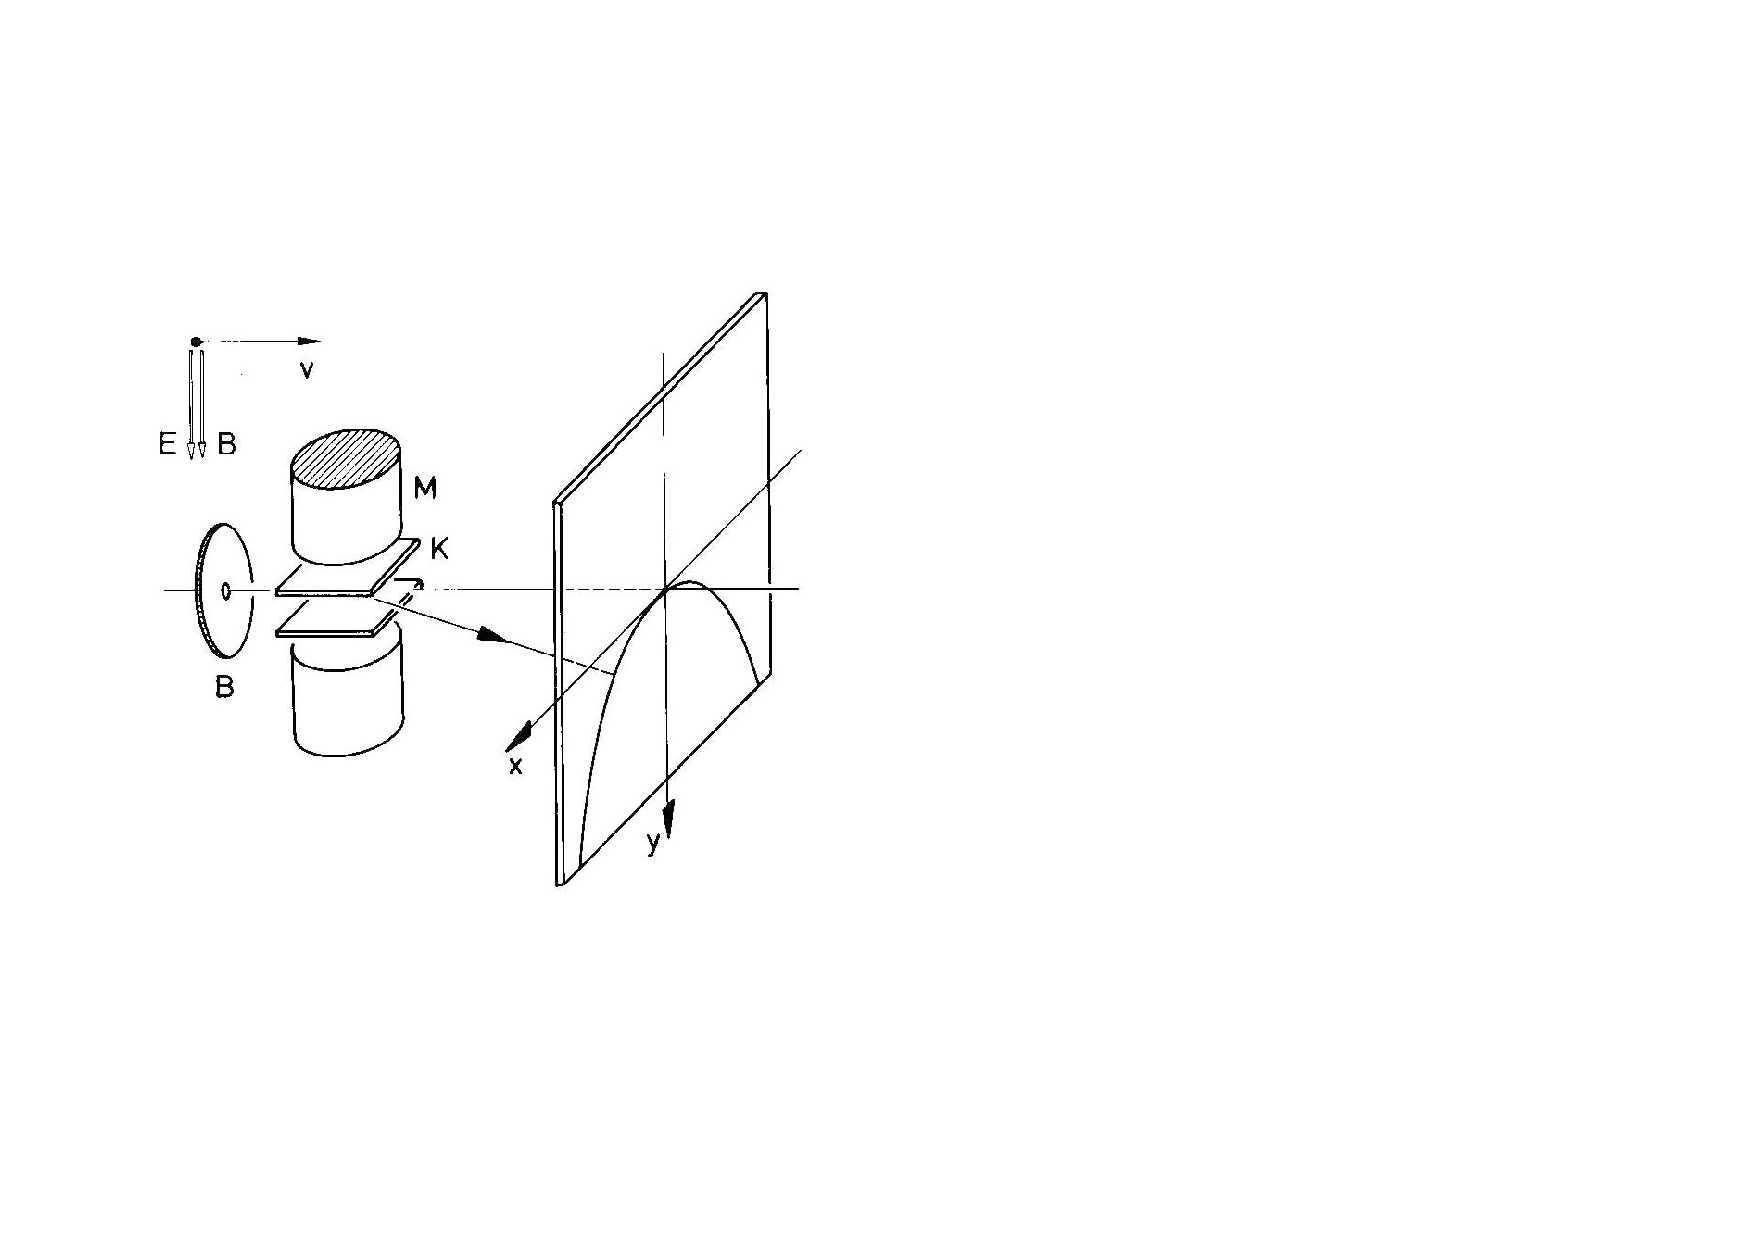
\includegraphics[width=0.5\textwidth]{fig/2-Parabelmethode.pdf}
% \caption{Prabelmethode, schematische Darstellung. Der durch die Blende $B$
% kollimierte Ionenstrahl wird durch den Magneten $M$ und den Kondensator $K$ in
% $x$- und $y$-Richtung abgelenkt. }
% H. Haken, H. C. Wolf, Atom- und Quantenphysik, S. 30 
% \end{SCfigure}
% 
% \begin{figure}[!htbp]
% 	\centering
% 	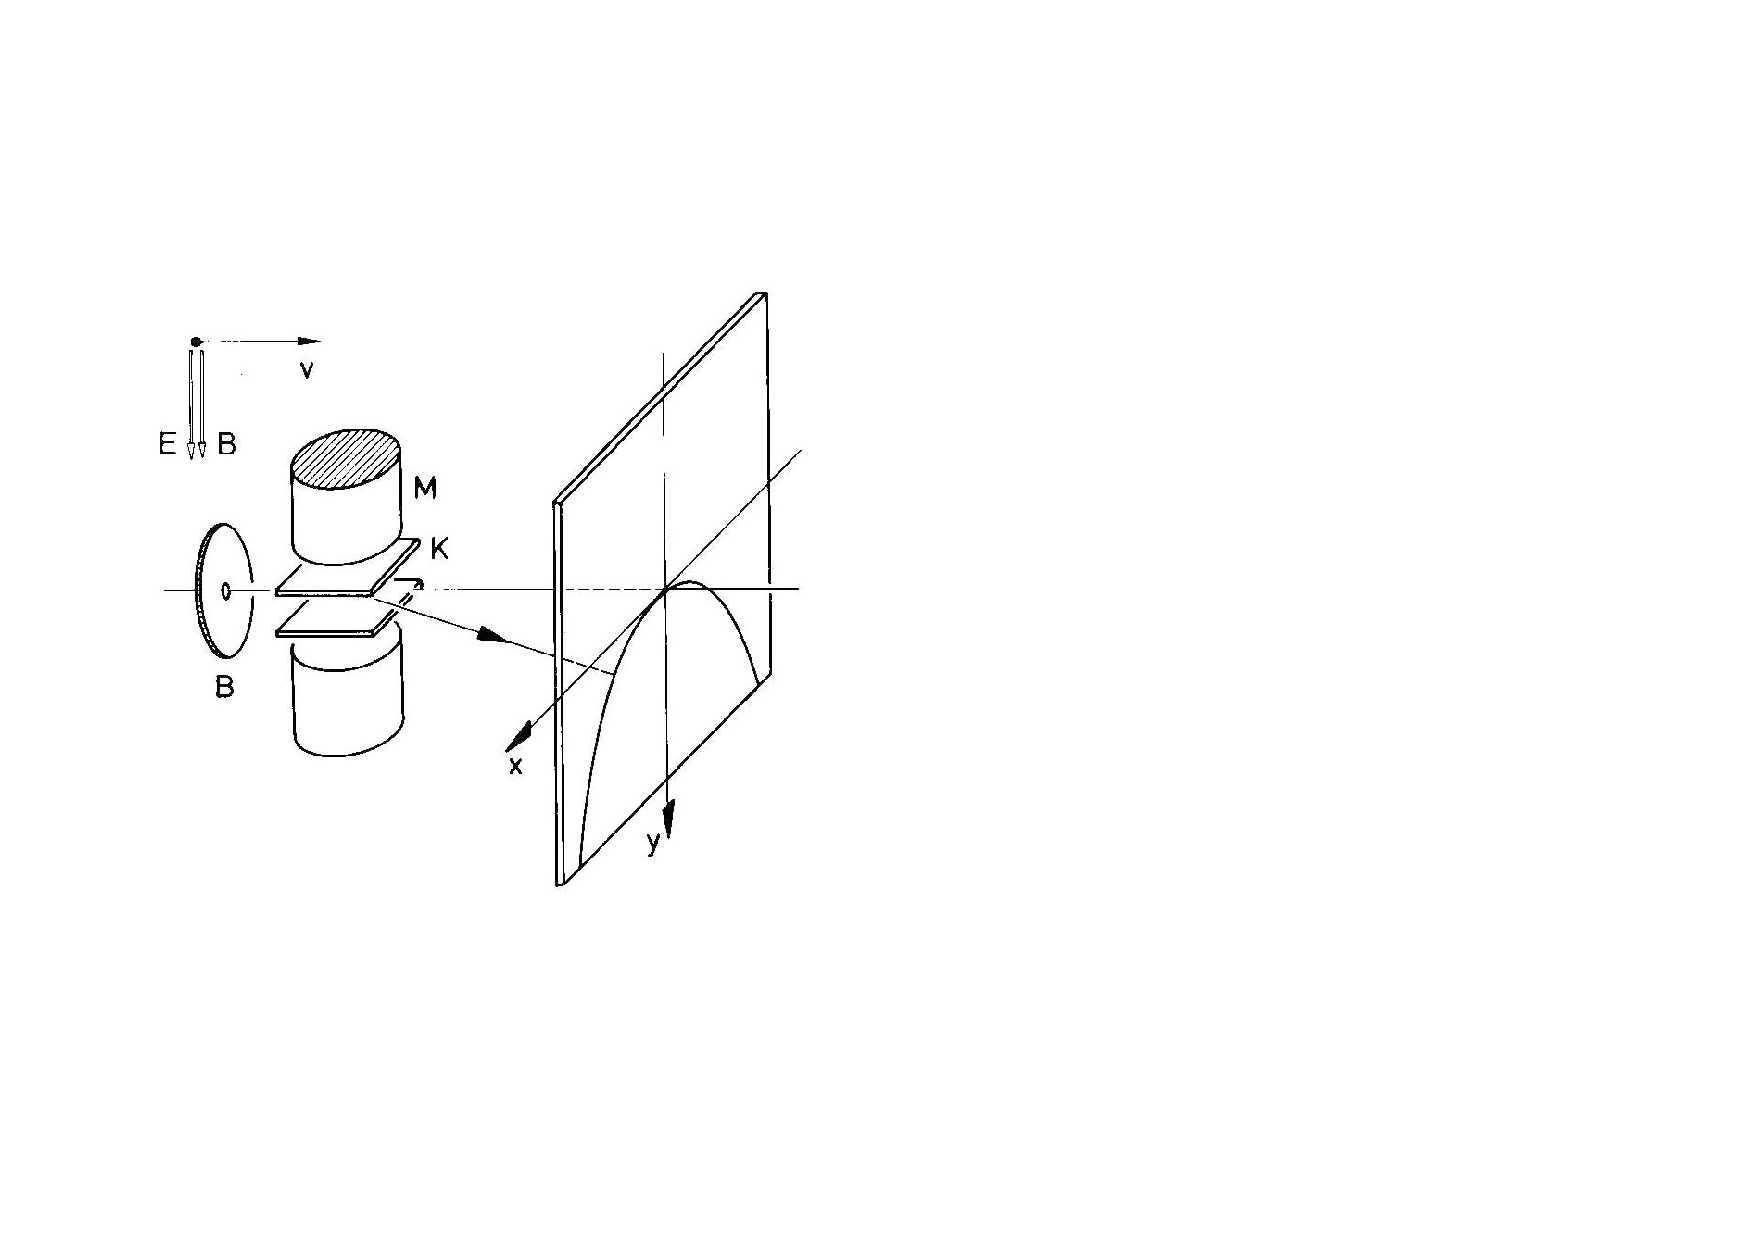
\includegraphics[width=\textwidth]{fig/2-Parabelmethode.pdf}
% \end{figure}

Der Teilchenstrahl durchquert einen Kondensator der Länge $L$, der von einem
Magneten umgeben ist. Elektrisches und Magnetisches Feld zeigen in
$y$-Richtung. Durch das elektrische Feld wirkt auf das Elektron die
Coulombkraft in $y$-Richtung,
\begin{align*}
\vec{F} = e\vec{E} \Rightarrow \ddot{y} = \frac{e}{m}E \Rightarrow y =
\frac{1}{2}\frac{eE}{m}t^2 = \frac{1}{2}\frac{eE}{m}\left(\frac{L}{v}\right)^2
= \frac{eEL^2}{4}\frac{1}{\frac{1}{2}mv^2}\sim \frac{1}{E_{\text{kin}}}\tag{*}
\end{align*}
Daher wird das Elektrische Feld auch ``Energiefilter'' genannt.

Durch das magnetische Feld wirkt auf das Elektron die Lorentzkraft in
$x$-Richtung,
\begin{align*}
&\vec{F} = e(\vec{v}\times\vec{B}) \Rightarrow F_x = evB = F_Z =
\frac{mv^2}{r}\\
\Rightarrow & \text{Kreisbahn mit Radius } r=\frac{mv}{eB}.
\end{align*}
Mit $x<<r$ erhalten wir so
\begin{align*}
a = \frac{evB}{m} \Rightarrow x = \frac{1}{2}at^2 =
\frac{1}{2}\frac{evB}{m}\frac{L^2}{v^2} = \frac{eBL^2}{2}\frac{1}{mv} \sim
\frac{1}{p}.
\end{align*}
Daher wird das magnetische Feld auch ``Impulsfilter'' genannt. Lösen wir den
Term nach $v$ auf und setzen in (*) ein, erhalten wir
\begin{align*}
y = \frac{2E}{L^2B^2}\frac{m}{e}x^2,
\end{align*}
unabhängig von der Geschwindigkeit $v$.

\rfigure[!htpb][0.45]%
	{2-ZerlegungIonenGemisch.pdf}%
	{\HakenWolf, S. 31}%
	{Zerlegung eines Gemisches von Kohlenwasserstoff-Ionen mit der Thomsonschen
	Parabelmethode. Zur Eichung benutzt man Ionen bekannter Masse. Die Intensität
	der einzelnen Parabelstücke entspriccht der relativen Häufigkeit der
	betreffenden Ionen des Gemisches.}

Mit diesem Versuch war auch erstmals die spezifische Ladung messbar,
\begin{align*}
\frac{e}{m} = 1.75\cdot 10^{11} \frac{\mathrm{c}}{\mathrm{kg}}.
\end{align*}

\begin{bemn}
Für große Geschwindigkeiten $v$ (d.h. kleine $x$ und $y$) ergibt sich eine
relativistische Abweichung
\begin{align*}
y = \frac{2E}{L^2B^2}\frac{m}{e}x^2\frac{1}{\sqrt{1-\frac{v^2}{c^2}}}.
\end{align*}
Sie wurde bereits 1902 von Kaufmann\footnote{Walter Kaufmann (* 5. Juni 1871
in Elberfeld; † 1. Januar 1947 in Freiburg im Breisgau) war ein deutscher
Physiker.} beobachtet, jedoch ohne Erklärung.\maphere
\end{bemn}

Kurz darauf (1908) erhielt Rutherford den Nobelpreis für Chemie für die
Entdeckung des $\alpha$-Zerfalls. Die Schwierigkeit hierbei war der Nachweis,
dass $\alpha$-Teilchen in der Tat Heliumkerne sind. Aufgrund ihrer hohen
Geschwindigkeit ließen sie sich durch elektrische Felder nicht maßgeblich
ablenken. Verwendet man jedoch eine Nebelkammer gefüllt mit Helium, sieht man,
dass beim Stoß der $\alpha$-Teilchen mit den Teilchen in der Nebelkammer ein
90° Winkel gebildet wird, d.h. $\alpha$-Teilchen und Helium haben dieselbe
Masse.


\rfigure[!htpb][0.35]%
	{2-Nebelkammer.pdf}%
	{\HakenWolf, S. 43}%
	{Nebelkammer-Aufnahme von $\alpha$-Teilchen. Man sieht Stoßprozesse mit dem
	Füllgas, links mit Wasserstoff, rechts mit Helium. Im Wasserstoff erleidet das
	treffende $\alpha$-Teilchen nur eine geringe Ablenkung, bei Helium dagegen ist
	der Winkel zwischen Bahnen von Streuteilchen und gestoßenem Atom $90^\circ$,
	weil beide die gleiche Masse haben.}

Rutherford verwendete daraufhin in seinen Streuexperimenten $\alpha$-Teilchen,
die er auf eine Goldplatte schoß. Er beobachtete, unter welchem Winkel $\th$
wie viele Ereignisse registriert werden.
\begin{figure}[!htbp]
  \centering
\begin{pspicture}(0,-1.7092611)(6.773818,1.7780532)
\pscircle(1.0171875,0.16){0.37}
\psline[linestyle=dotted,dotsep=0.16cm](1.5671875,0.09)(3.3471875,0.07)
\psline(3.6,0.15)(3.6,1.57)
\psline(3.6,-0.01)(3.6,-1.37)
\psline{->}(3.6871874,0.07)(4.5871873,0.07)
\psline[linestyle=dotted,dotsep=0.16cm](1.5671875,0.41)(3.2471876,1.09)
\psline[linestyle=dotted,dotsep=0.16cm](1.5471874,-0.19)(3.1671875,-0.83)
\psline[linecolor=yellow](4.7871876,0.79)(4.7671876,-0.47)
\psline[linestyle=dotted,dotsep=0.16cm](4.8671875,0.07)(6.5471873,0.07)
\psarc(5,0.08){0.53}{0}{50}
\psline[linecolor=darkblue]{->}(4.8871875,0.15)(6.1471877,1.07)
\psarc(4.6,0.0){1.97}{300.96375}{63.17802}

\rput{36.360546}(2.0732305,-3.5930915){\psframe[linewidth=0.04,dimen=outer](6.7671876,1.47)(6.2471876,1.25)}

\rput(1.0,-0.75){Quelle: Radon}
\rput(4.7,-0.75){Target}
\rput(3.6,-1.58){Blende}

\rput(2.6,0.32){\color{gdarkgray}$\alpha^{++}$}
\rput(5.3,0.25){\color{gdarkgray}$\th$}
\end{pspicture} 
  \caption{Versuchsaufbau: Rutherfordstreuung.}
\end{figure}


Zum Zeitpunkt der Durchführung des Experiments ging man noch vom
Thomsonschen Atommodell aus.
\begin{enumerate}[label=\arabic{*}.)]
  \item Elektronen sind in allen Elementen enthalten.
  \item Die Ladungsverteilung im Atom ist homogen, Protonen, Neutronen und
  Elektronen verteilen sich so, dass die elektrostatische Anziehung minimiert
  wird.
\end{enumerate}

\sfigure[!htpb]%
	{2-AtommodellThomson.pdf}
	{}
	{Das Elektron als elementarer Baustein der Materie.}

Rutherford stellte in seinem Versuch jedoch auch bei großen Winkeln $\th>90°$
noch Ablenkung fest, was darauf schließen ließ, dass der Atomkern
einen viel kleineren Radius als das Atom selbst haben muss.

\begin{figure}[!htbp]
	\centering
	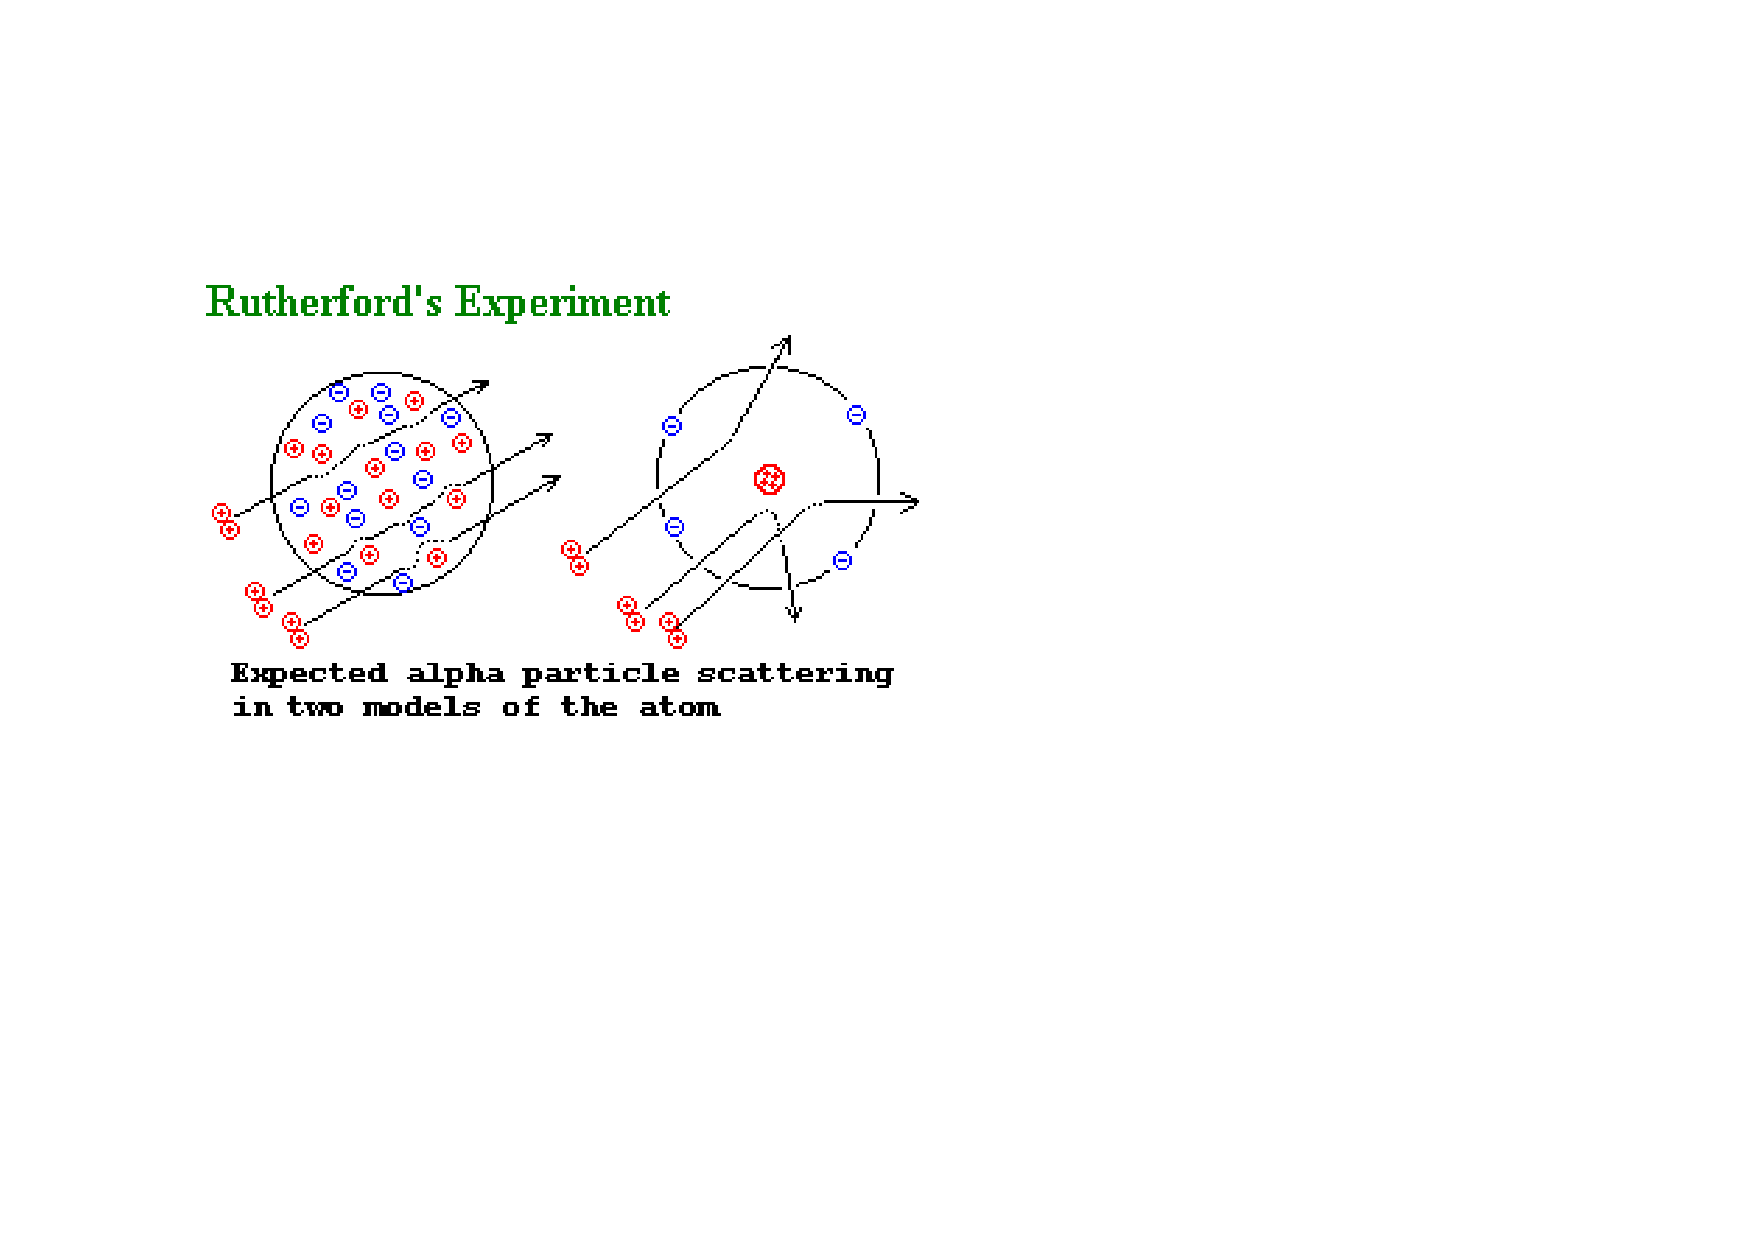
\includegraphics[width=0.49\textwidth]{fig/2-RutherfordStreuungErwartung.pdf}
	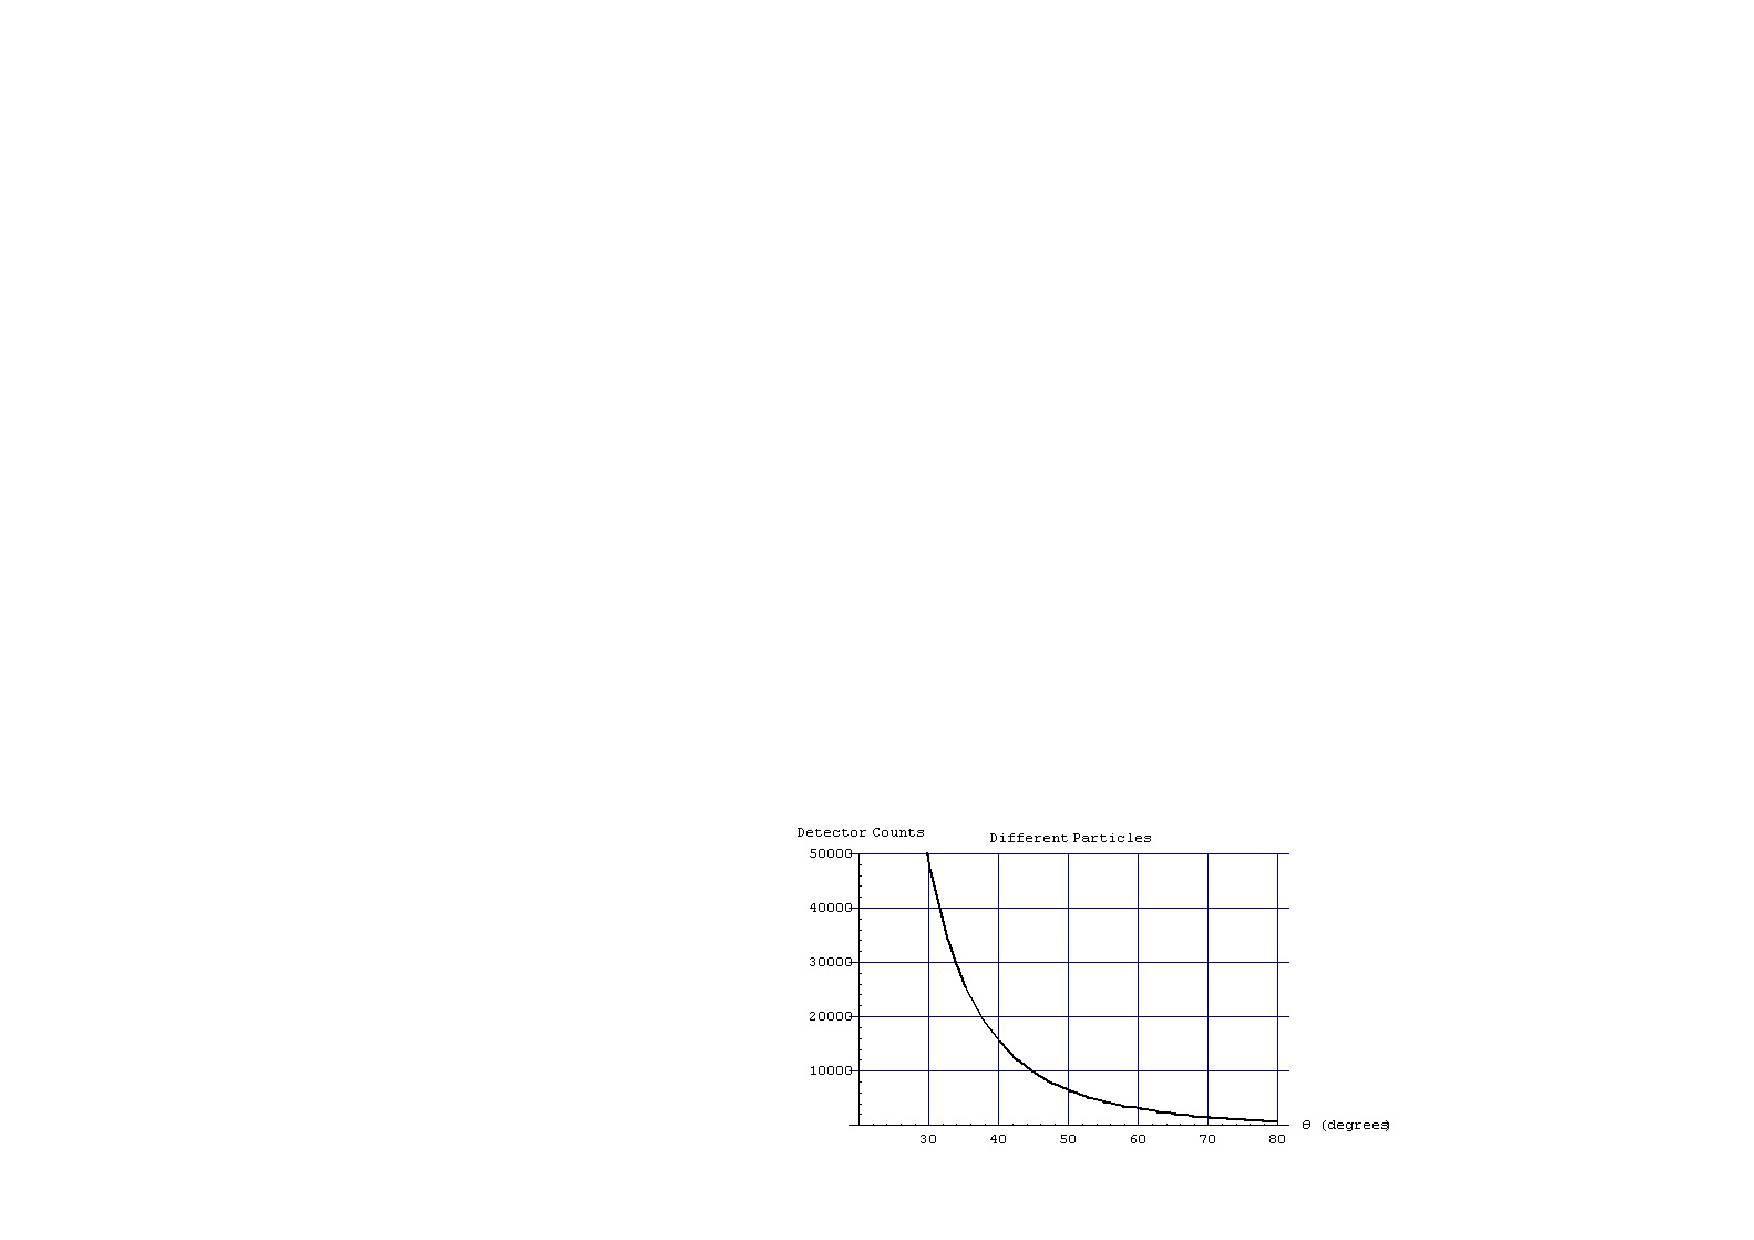
\includegraphics[width=0.49\textwidth]{fig/2-RutherfordExperimentWinkelabhaengigkeit.pdf}
	\caption{Modellvorstellungen zur $\alpha$-Teilchen Streuung (links) und real
	gemessene Intensität in Abhängigkeit vom Winkel (rechts).}
\end{figure}

\begin{figure}[!htbp]
	\centering
	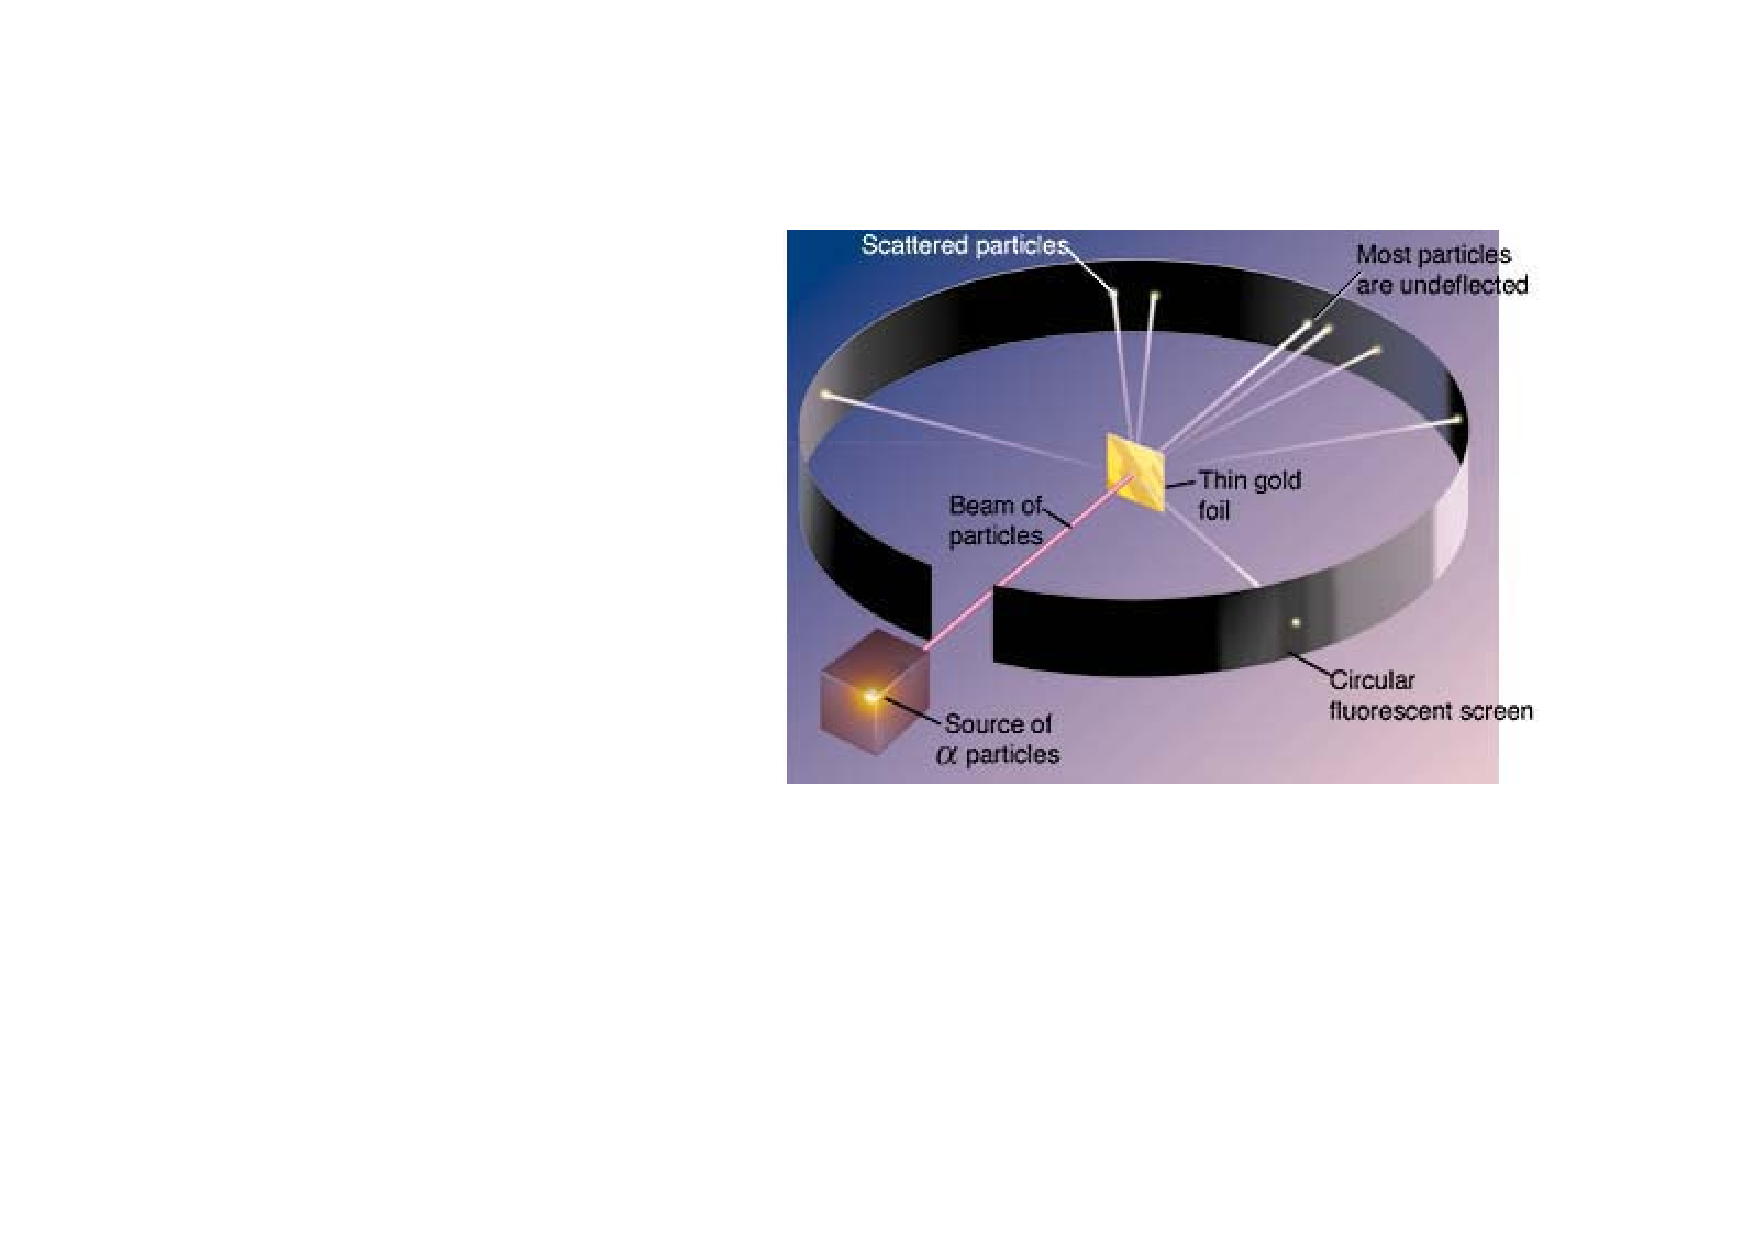
\includegraphics[width=\textwidth]{fig/2-RutherfordExperimentAufbau.pdf}
\end{figure}

\subsubsection{Rutherford'sche Streuformel}
	
Um die Ergebnisse zu formulieren benötigen wir noch einige Begriffe.
\begin{defnn}
Der \emph{Wirkungsquerschnitt} $\sigma$ ist ein Maß für die Wahrscheinlichkeit
einer Reaktion. Die Zahl der Rekationen ist gegeben durch,
\begin{align*}
N = j\cdot n\cdot\sigma,
\end{align*}
wobei $j$ die Stromdichte der einfallenden Teilchen und $n$ die Zahl der
Targetteilchen bezeichnet. $\sigma$ hat hier die Einheit einer Fläche.\fishhere
\end{defnn}

Wir sehen, dass $\sigma$ die relevanten Informationen über die
einzelnen Reaktionen enthält.

\begin{bemn}
Für ein Target aus Kugelteilchen ist $\sigma = \pi R^2$. Bei Coulomb-Stößen
geht jedoch die geometrische Anschauung verloren, denn die Wechselwirkung hat
$\infty$-Reichweite. D.h. der Wirkungsquerschnitt divergiert im Raum. Man geht
daher zu differentiellen Größen über,
\begin{align*}
\dot{N}(\th) = j\cdot n\cdot\sigma(\th)\Delta\Omega,
\end{align*}
wobei $\sigma$ hier einen differentiellen Wirkungsquerschnitt bezeichnet und
$\Delta \Omega$ einen Raumwinkel.\maphere
\end{bemn}

\sfigure[htbp][0.6]%
	{2-DefinitionDifferentiellerWirkungsquerschnitt.pdf}%
	{}
	{Zur Definition des differentiellen Wirkungsquerschnitts.}

Rutherford hat die Winkelabhängigkeit des differentiellen Wirkungsquerschnitts
empirisch bestimmt. Um den Ausdruck für $\sigma$ theoretisch herzuleiten,
verwendet man Drehimpulserhaltung,
\begin{align*}
&\vec{L} = \mu \left(\vec{r}\times\vec{v}\right) = \const,\tag{*}\\
\Rightarrow & \abs{\vec{L}} = \mu r^2 \frac{\diffd \ph}{\dt} = \mu v_0 b,
\end{align*}
sowie Impulserhaltung,
\begin{align*}
\abs{\vec{p}} = m v_0 = \const.
\end{align*}

\sfigure[H]%
	{2-SkizzeRutherfordStreuformel.pdf}%
	{}
	{Zur Herleitung der Winkelabhängigkeit.}

Die Bewegung findet nur in der $x,y$-Ebene statt, welche $\bot$ zu $\vec{L}$
ist. Setze $a:= \frac{Z_1Z_2 e^2}{4\pi\ep_0}$ und berechne $p_y$,
\begin{align*}
\dot{v}_y &= \frac{1}{\mu} F_y = \frac{1}{\mu}\frac{a}{r^2}\sin\ph
\overset{*}{=} \frac{1}{\mu}a\sin\ph \frac{\dph}{\dt}\frac{1}{v_0 b}.\\
\Rightarrow 
v_y &= \int\limits_{-\infty}^\infty \dot{v}_y \dt = \int\limits_{0}^{v_0\sin\th}
\diffd v_y = v_0\sin\th
= \frac{a}{\mu v_0 b}\int\limits_{-\infty}^\infty \sin\ph \frac{\dph}{\dt}\dt\\
&= \frac{a}{\mu v_0 b}\int\limits_{0}^{\pi-\th} \sin\ph \dph
= \frac{a}{\mu v_0 b}(1+\cos\th).
\end{align*}
Wir erhalten somit,
\begin{align*}
\cot \frac{\th}{2} = 
\frac{1+\cos\th}{\sin\th}=
\mu v_0^2\frac{b}{a} = 2 E_0 \frac{b}{a} = 2 \frac{E_0}{V_\text{pot}(b)},
\end{align*}
d.h. wir können $\th$ in Abhängigkeit von $b$ darstellen. Invertieren ergibt,
\begin{align*}
b(\th) = \frac{D}{2}\cot\frac{\th}{2},\qquad D=\frac{1}{4\pi\ep_0}\frac{Z_1Z_2e^2}{E_0}.
\end{align*}
Mit $\sigma(\th) = \frac{b}{\sin\th}\abs{\frac{\db}{\dth}}$ erhalten wir so für
den differentiellen Wirkungsquerschnitt,
\begin{align*}
\sigma(\th) =
\left(\frac{D}{4}\right)^2\frac{1}{\sin^4\left(\frac{\th}{2}\right)}.
\end{align*}
Die $\sin^{-4}\left(\frac{\th}{2}\right)$ Proportionalität ist
charakteristisch für die Rutherford Streuung.

Im Streuexperiment erwartet man also
\begin{align*}
N(\th) = j\cdot n \cdot C \cdot \Delta\Omega
\sin^{-4}\left(\frac{\th}{2}\right).
\end{align*}
Mithilfe von $C$ kann man $\frac{Z_1Z_2}{E_0}$ bestimmen.

\subsubsection{Kernradienbestimmung}
Bei der Messung von $\sigma$ wird in der Regel der Winkel $\th$ variiert unter
dem der Detektor misst. In großen Beschleunigeranlagen kann man auch den Winkel
konstant halten und die kinetische Energie variieren, um die
$\frac{1}{E_\text{kin}}$-Abhängigkeit zu verifizieren. Die Formel für den
differentiellen Wirkungsquerschnitt wurde experimentell für
\begin{align*}
E_\text{kin} < 5MeV,\qquad \th<150°,
\end{align*}
bestätigt. Für den Stoßparameter $b$ gilt,
\begin{align*}
b(\th) = \frac{D}{2}\cot\frac{\th}{2} < 6\cdot 10^{-15}m.
\end{align*}
Wir erhalten so eine obere Grenze für den Kernradius.
\begin{align*}
R \approx r_0\cdot A^{1/3},\qquad r_0 = 1.3\cdot 10^{-15}m,
\end{align*}
wobei $A$ für die Nukleonenzahl steht. Der Kerndurchmesser liegt also im
Femtometerbereich und damit $5$ Größenordnungen unter dem Atomdurchmesser.
Außerdem sehen wir, dass bei großer Entfernung vom Kern das Potential gerade
wie ein Coulomb-Potential aussieht.

\rfigure[!htpb][0.4]%
	{2-KernCoulomb.pdf}%
	{\HakenWolf, S. 49}%
	{Kernkraft- und Coulombpotential.}

Wir wollen nun untersuchen, wie wir durch Messungen von
$\frac{\diffd\sigma}{\diffd\Omega}$ Aussagen über die Form des Potentials machen
können.

\rfigure[!htpb][0.4]%
	{2-StreuungAlphaElast.pdf}%
	{\FrauenfelderHenley, S. 171}%
	{Differentieller Wirkungsquerschnitt für die elastische Streuung von
	$\alpha$-Teilchen an ${}^{24}Mg$.}

% \begin{figure}[!htbp]
% 	\centering
% 	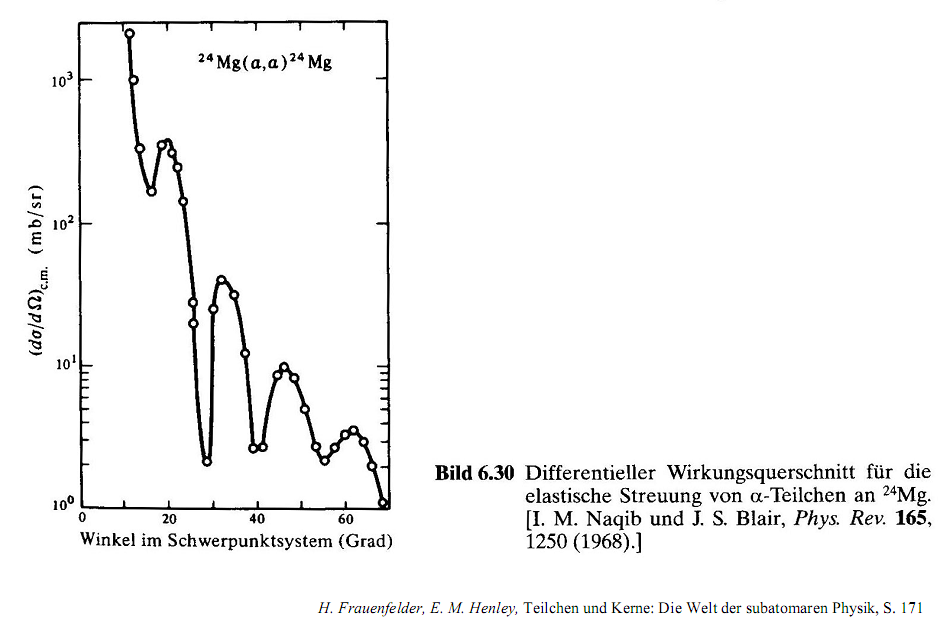
\includegraphics[width=\textwidth]{fig/2-StreuungAlphaElast.png}
% \end{figure}
Ähnlich wie bei Beugungsexperimenten in der Optik, tritt für bestimmte Winkel
$\th$ Resonanz im Kern auf und wir erhalten Beugungsmaxima. Verwenden wir verschiedene Teilchen als
Streuteilchen, erhalten wir Informationen über die verschiedenen
Wechselwirkungen (stark, schwach, elektromagnetisch).

Für geladene Streuteilchen muss die Energie hoch genug sein, um den Kern selbst
zu erreichen und zu untersuchen. Um Details im Kern aufzulösen, muss aber auch
ein neutrales Streuteilchen genug Energie haben. Im Bild der Optik muss die de
Broglie Wellenlänge des Streuteilchens viel kleiner sein als der Kern, um die
detailierte Struktur zu ``mikroskopieren''.
\begin{bspn}
\begin{enumerate}[label=\arabic{*}.)]
  \item Neutronen erfahren keine Coulomb Wechselwirkung. Das Beugungsmuster
  kommt nur durch starke Wechselwirkung zustande.

\rfigure[!htpb][0.5]%
	{2-StreuungNeutronenElast.pdf}%
	{\Stierstadt, S. 91}%
	{Winkelverteilung von an Atomkernen gestreuten Neutronen mit $2.2\cdot
	10^{-12}\mathrm{J} (14\mathrm{MeV})$ Primärenergie. Die durchgezogenen Kurven
	sind mit dem Modell berechnet.}

% \begin{figure}[!htbp]
% 	\centering
% 	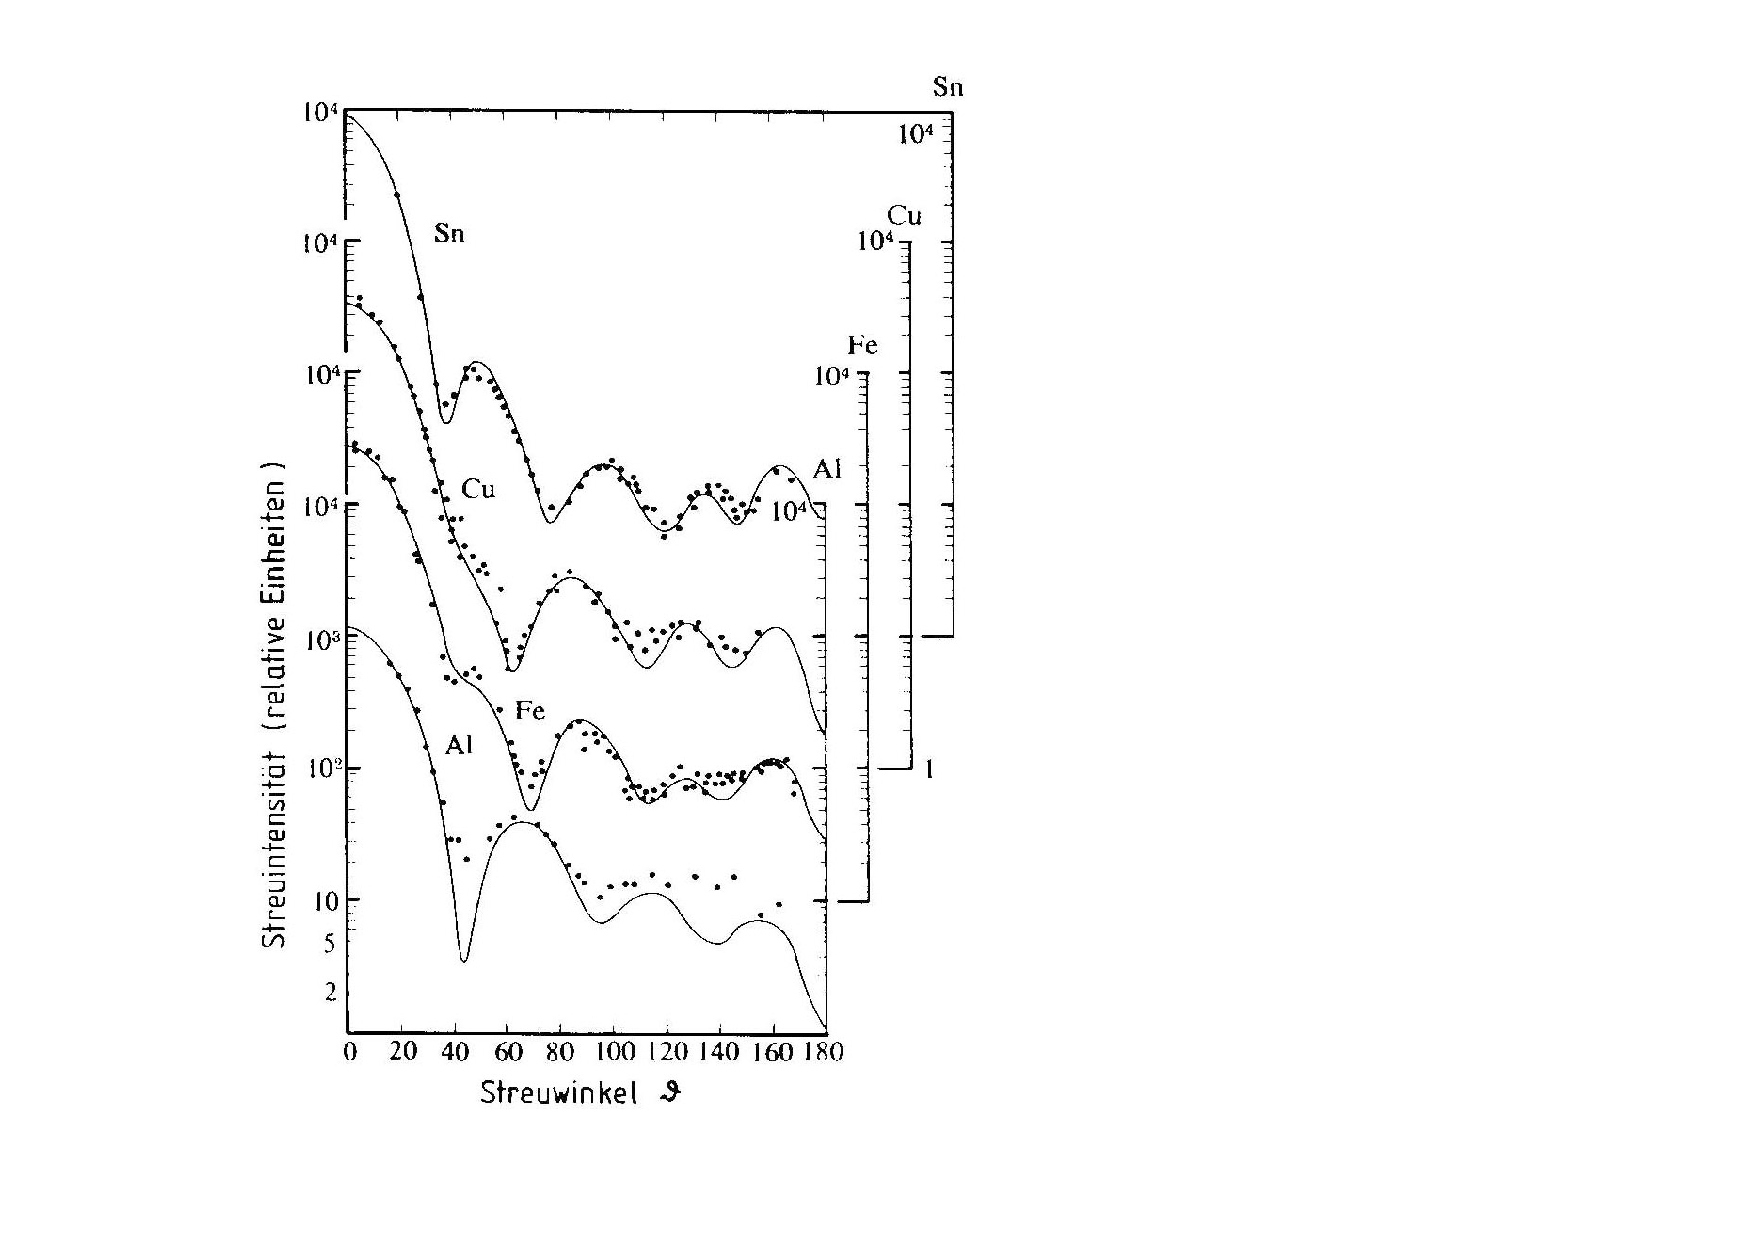
\includegraphics[width=\textwidth]{fig/2-StreuungNeutronenElast.pdf}
% \end{figure}
\item Elektronen erfahren nur Coulomb-Wechselwirkung.
\rfigure[!htpb][0.4]%
	{2-StreuungElektronElast.pdf}%
	{\KuckukKern, S. 27}%
	{Winkelverteilung elastisch gestreuter Elektronen an Kohlenstoff.}
\rfigure[!htpb][0.5]%
	{2-StreuungElektron2Elast.pdf}%
	{\BethgeWalter, S. 42}%
	{Elektronenstreuung an Uran, gemessen bei zwei Energien.}

% \begin{figure}[!htbp]
% 	\centering
% 	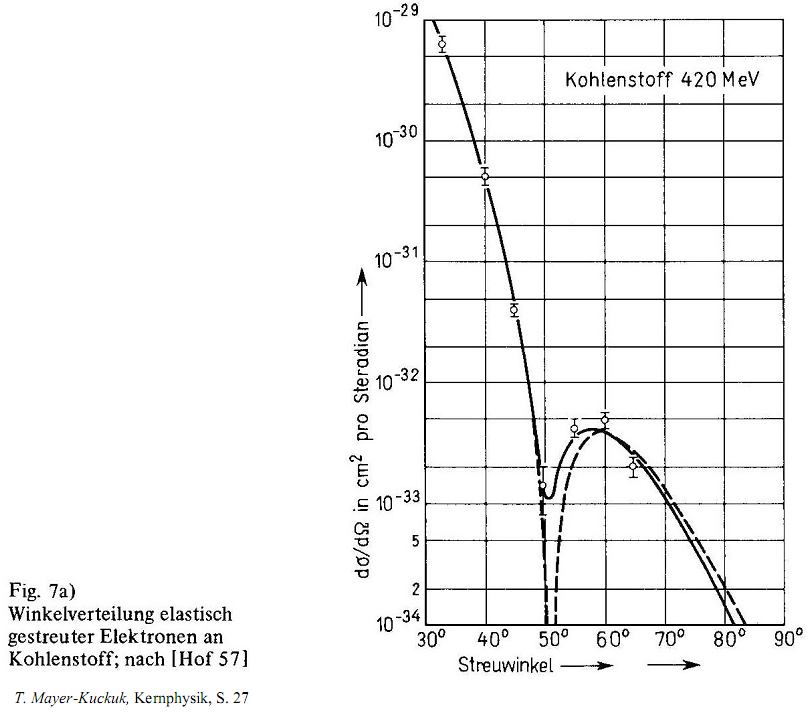
\includegraphics[width=\textwidth]{fig/2-StreuungElektronElast.png}
% \end{figure}
% \begin{figure}[!htbp]
% 	\centering
% 	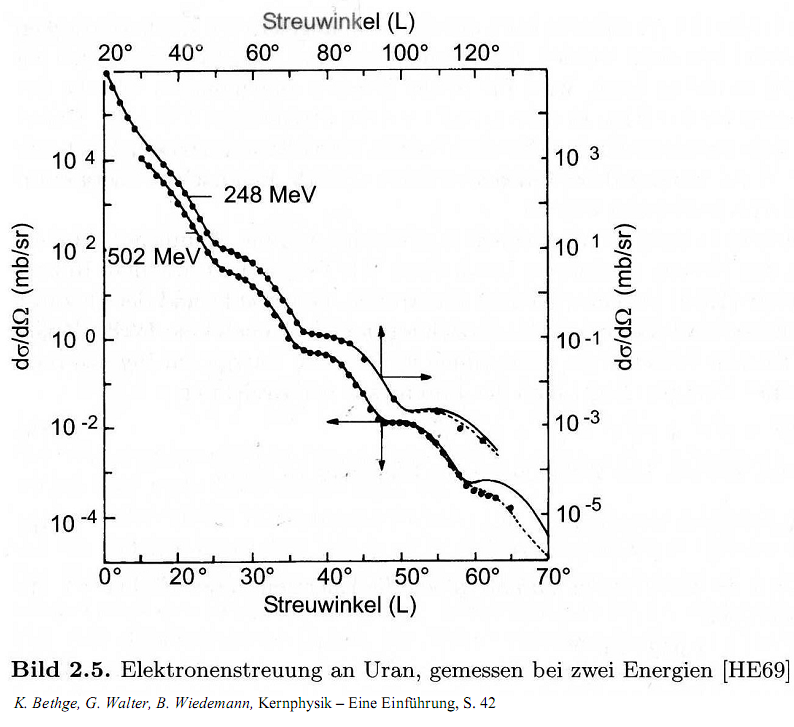
\includegraphics[width=\textwidth]{fig/2-StreuungElektron2Elast.png}
% \end{figure}
\item Die Messergebnisse zeigen, dass die Ladungsverteilung von der
Atommasse abhängt. Ist das Wasserstoffatom noch singulär, so hat Silizium
eine homogene Dichteverteilung. Schwere Kerne haben in etwa alle die gleiche
homogene Kerndichte.

\sfigure[!htpb]%
	{2-StreuungLadungsvert.pdf}%
	{\BethgeWalter, S. 44}%
	{\label{fig:radlad}Radiale Ladungsverteilungen einiger Atomkerne. Diese Daten
	werden aus der Inversion der Streudaten gewonnen, ähnlich wie man aus dem
	Fernfeldbeugungsbild in der Optik das beugende Objekt rekonstruieren kann.}

% \begin{figure}[!htbp]
% 	\centering
% 	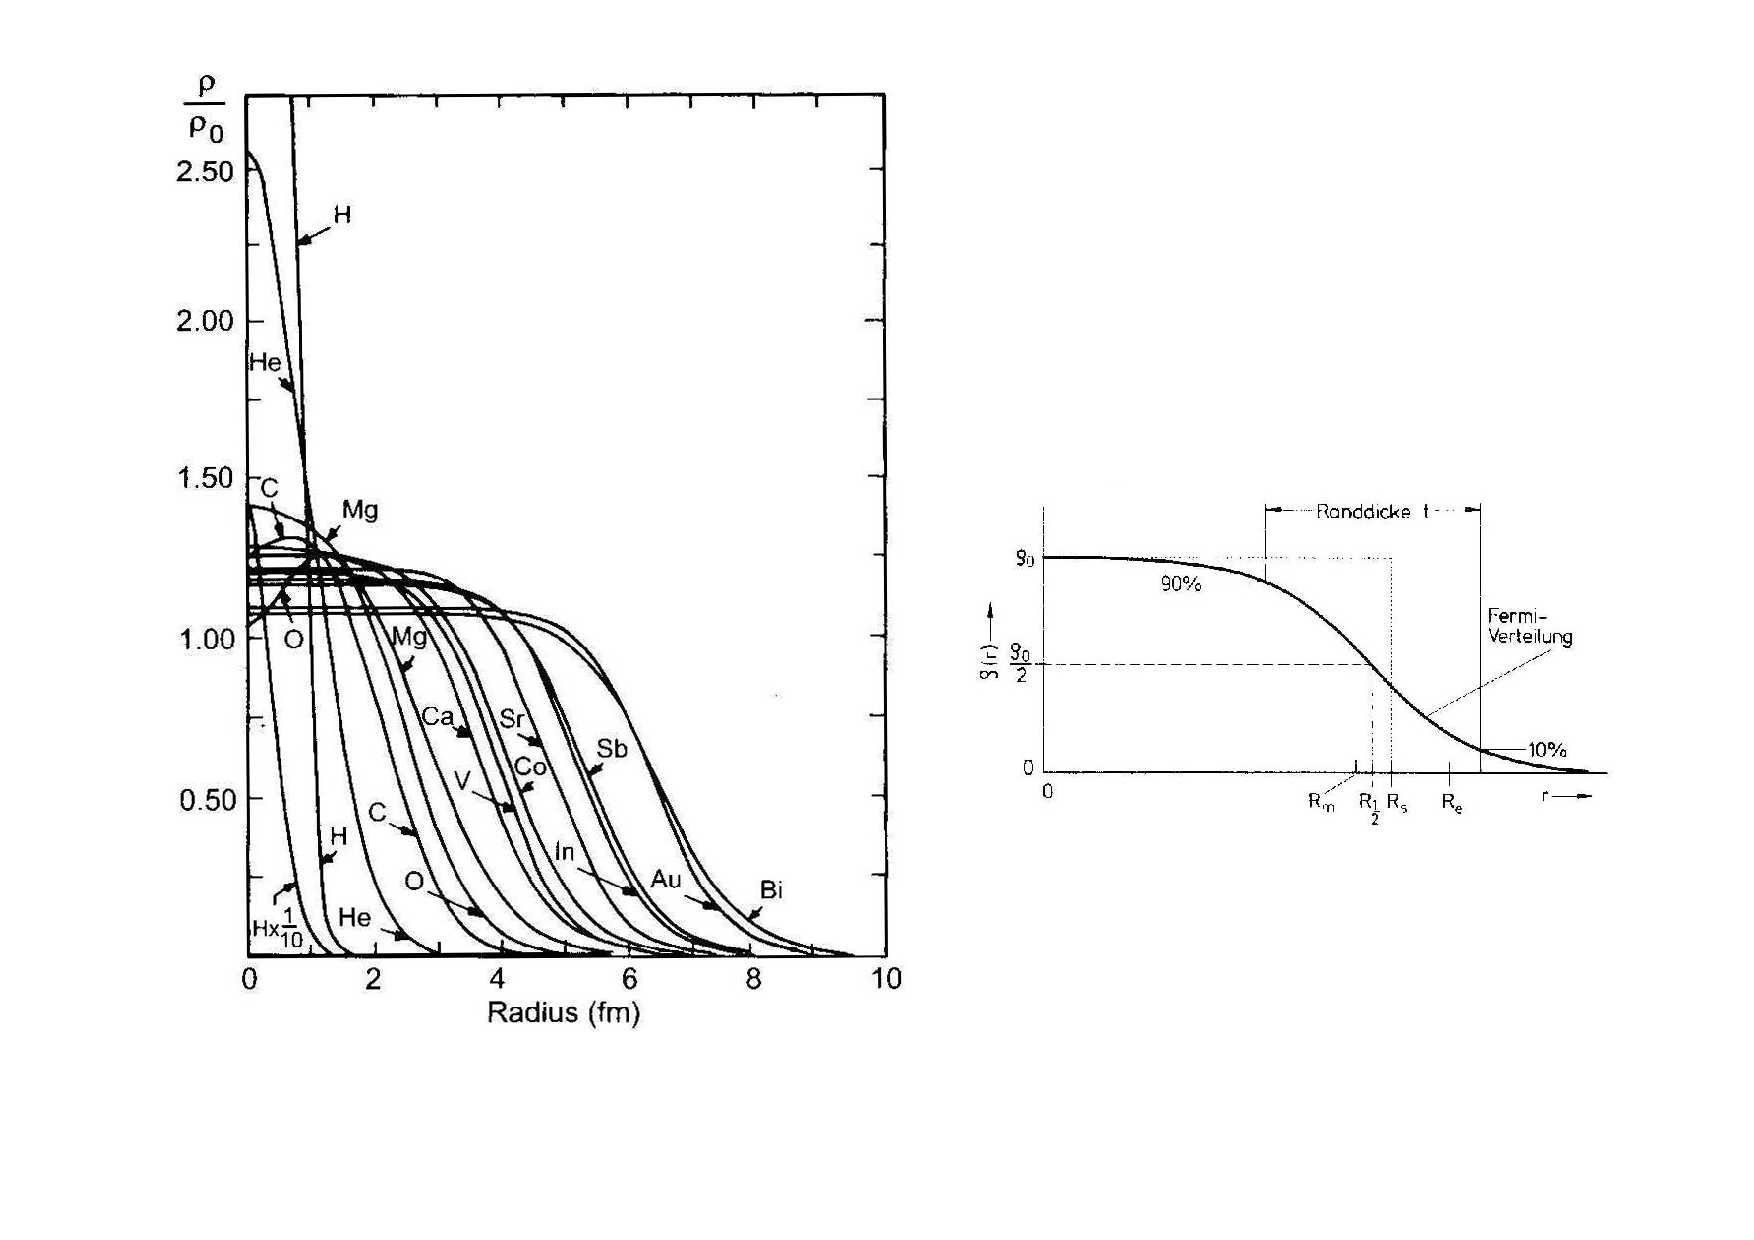
\includegraphics[width=\textwidth]{fig/2-StreuungLadungsvert.pdf}
% \end{figure}
\end{enumerate}
\end{bspn}
\begin{bemn}
Streuversuche kann man als Mikroskopie mit Materiewellen verstehen. Es gelten
die selben Auflösungsgesetze wie in der optischen Mikroskopie, d.h. die
Auflösung $\entspr$ Wellenlänge, wobei hier die De-Broglie Wellenlänge
\begin{align*}
\lambda_{dB} = \frac{h}{p},
\end{align*}
mit dem relativistischen Impuls $p$ gemeint ist. Für eine vorgegebene
$E_\text{kin}$ erhalten wir aus dem $p$-Skalarprodukt,
\begin{align*}
&E^2 = p^2c^2 +m_e^2c^4 = (E_\text{kin}+m_ec^2)^2.\\
\Rightarrow & p = \frac{1}{c}\sqrt{(E_\text{kin}+m_ec^2)^2 - m_e^2c^4}
= \frac{1}{c}\sqrt{E_\text{kin}^2+2E_\text{kin}m_ec^2+m_e^2c^4 - m_e^2c^4}
\\ &= \frac{1}{c}\sqrt{E_\text{kin}(E_\text{kin}+2m_ec^2)},\\
\Rightarrow & \lambda_{dB} =
\frac{hc}{\sqrt{E_\text{kin}}\sqrt{E_\text{kin}+2m_ec^2}}.
\end{align*}
Für $E_\text{kin}=100 \mathrm{MeV}$ ergibt sich $\lambda_{dB}\approx
10^{-14}\mathrm{m} = 10 \mathrm{fm}$, was noch zu wenig für Kernauflösung ist.
Bei der Verwendung von Elektronen werden aufgrund der geringen Masse für
Kernauflösung sehr hohe Energien benötigt. Während bei $\alpha$-Teilchen
bereits eine Energie von $5 \mathrm{MeV}$ ausreicht, sind bei Elektronen $500
\mathrm{MeV}$ notwendig.\maphere
\end{bemn}

\sfigure[H][0.6]%
	{2-WirkungsquerschnittUndLadungsverteilung.pdf}%
	{\FrauenfelderHenley, S. 163}
	{Wirkungsquerschnitt und Ladungsverteilung. Das Beugungsminimum im
	Wirkungsquerschnitt der schweren Kerne weist auf die wohldefinierte
	Kernoberfläche hin. Nukleonen dagegen besitzen eine langsam abnehmende
	Ladungsdichte an der Oberfläche.}

\subsection{Inelastische Streuung, Quarks und QCD}
Geht man zu Streuteilchen mit noch höherer Energie über und betrachtet die
verbleibenden Energie der gestreuten Teilchen, kann man Aufschluss über die
innere Struktur der Kerne und Nukleonen erhalten. Wir betrachten dazu die
Energie der gestreuten Teilchen als Funktion der Energie.
 
Bei Protonen kann man so feststellen, dass innere Anregungszustände existieren
(vgl. Spektrallinien) und diese daher eine innere Struktur besitzen, also aus
kleineren Teilchen aufgebaut sind.

\begin{figure}[!htpb]
\centering
\begin{minipage}{1\linewidth}%
	\renewcommand{\footnoterule}{}%
	\centering%
	\begin{pspicture}(0,-3)(11,5)
	\rput(5,0){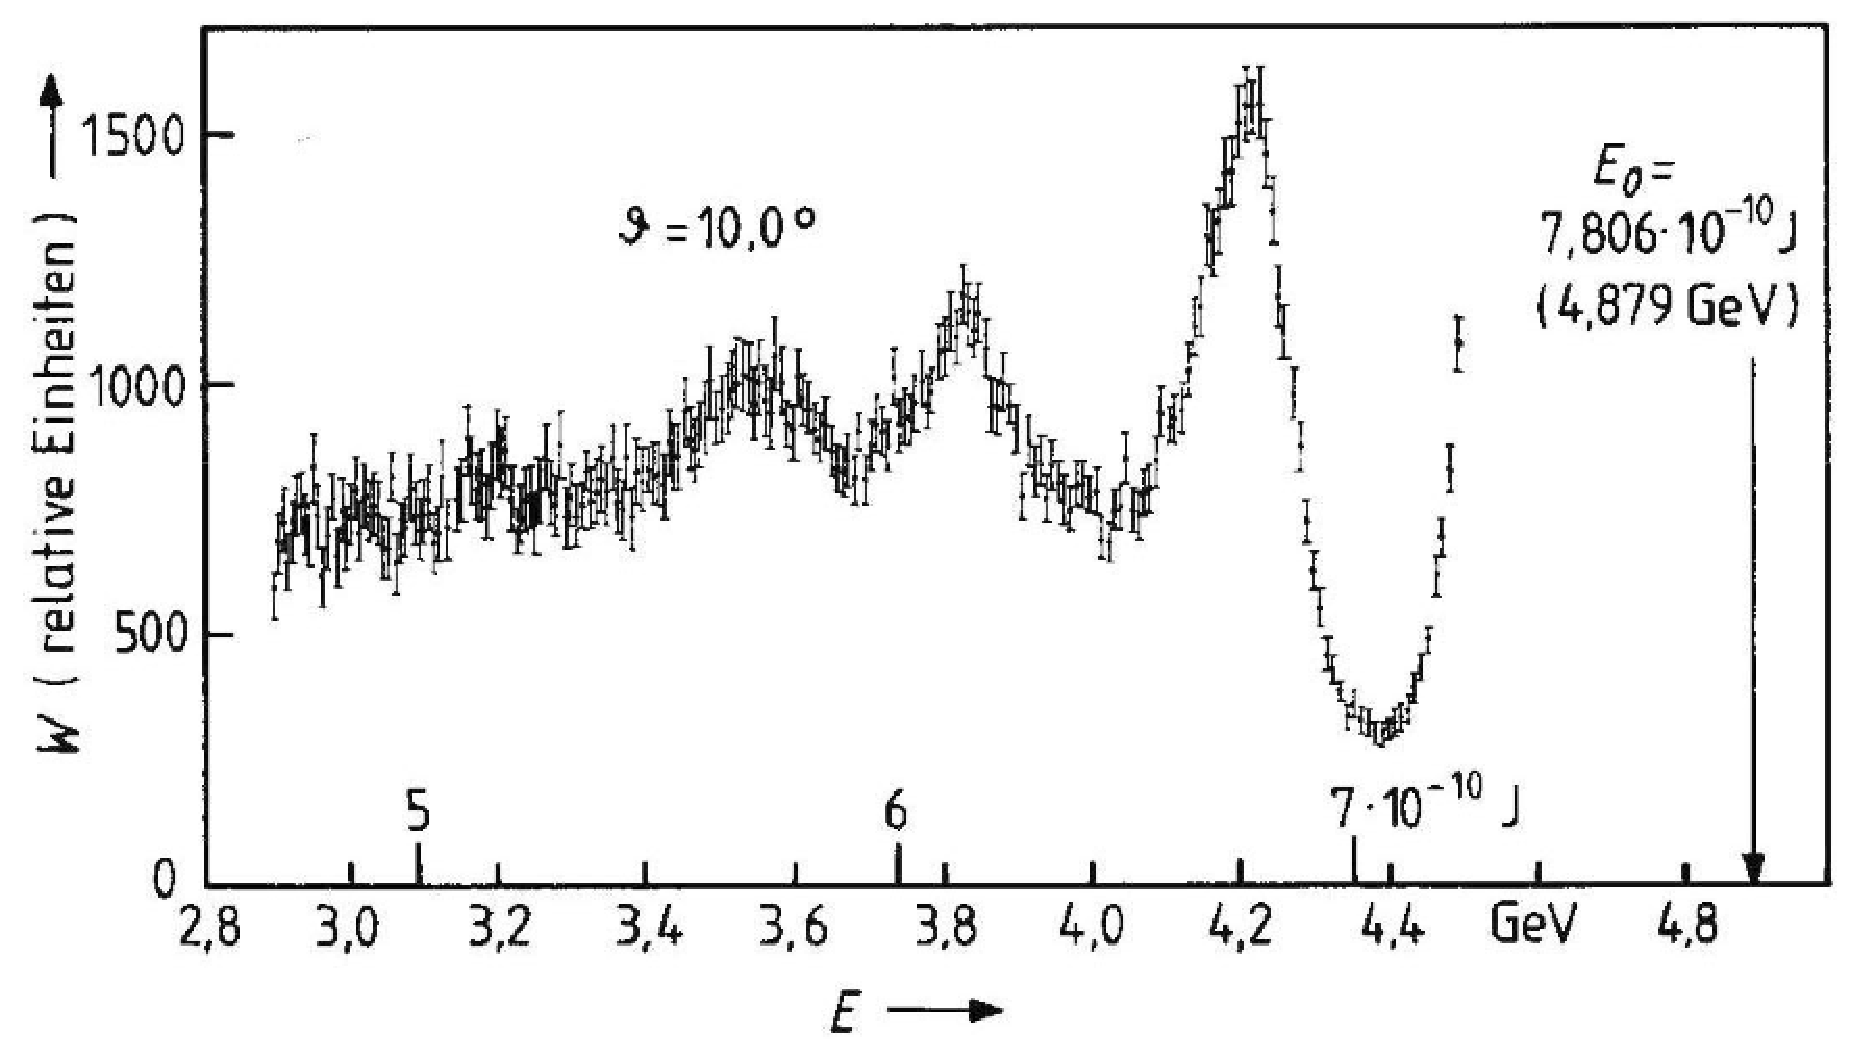
\includegraphics[width=10cm]{fig/2-InelastProton.eps}}
	\psline[linecolor=darkblue]{<-}(6.8,3)(6.8,4.2)
	\psline[linecolor=darkblue]{<-}(9.45,3)(9.45,4.2)
	\psline{<->}(7,3.6)(9.2,3.6)
	\rput(8.1,4){\color{gdarkgray}$\Delta E$}
	\rput(6.4,4.7){\color{gdarkgray}inelastischer Peak}
	\rput(9.6,4.7){\color{gdarkgray}elastischer Peak}
	\end{pspicture}
	\footnotetext{\textit{K. Stierstadt}, Physik der Materie, S. 28}
\end{minipage}
\caption{Nachweis der inneren Struktur von Protonen durch Streuung von
hochenergetischen Elektronen. Bei den inelastischen Peaks ist jeweils eine
Energie $\Delta E$ vom Target absorbiert worden, um in einen angeregten Zustand
überzugehen.}
\end{figure}

% \sfigure[!htpb]%
% 	{2-InelastProton.pdf}%
% 	{\textit{K. Stierstadt}, Physik der Materie, S. 28}
% 	{Nachweis der inneren Struktur von Protonen durch Streuung von
% 	hochenergetischen Elektronen.}

Für bestimmte Energien der streuenden Teilchen tritt Resonanz auf, d.h. im
Proton werden Energieniveaus mit dieser bestimmten Energie angeregt. 
Übersetzten wir das Energiemuster in ein Anregungsschema, sehen wir, dass
$p^+$ und $n^0$ dieselben Anregungsspektren besitzen. Ein analoges Ergebnis
erhalten wir für $\Delta$-Teilchen. \begin{figure}[!htbp]
	\centering
	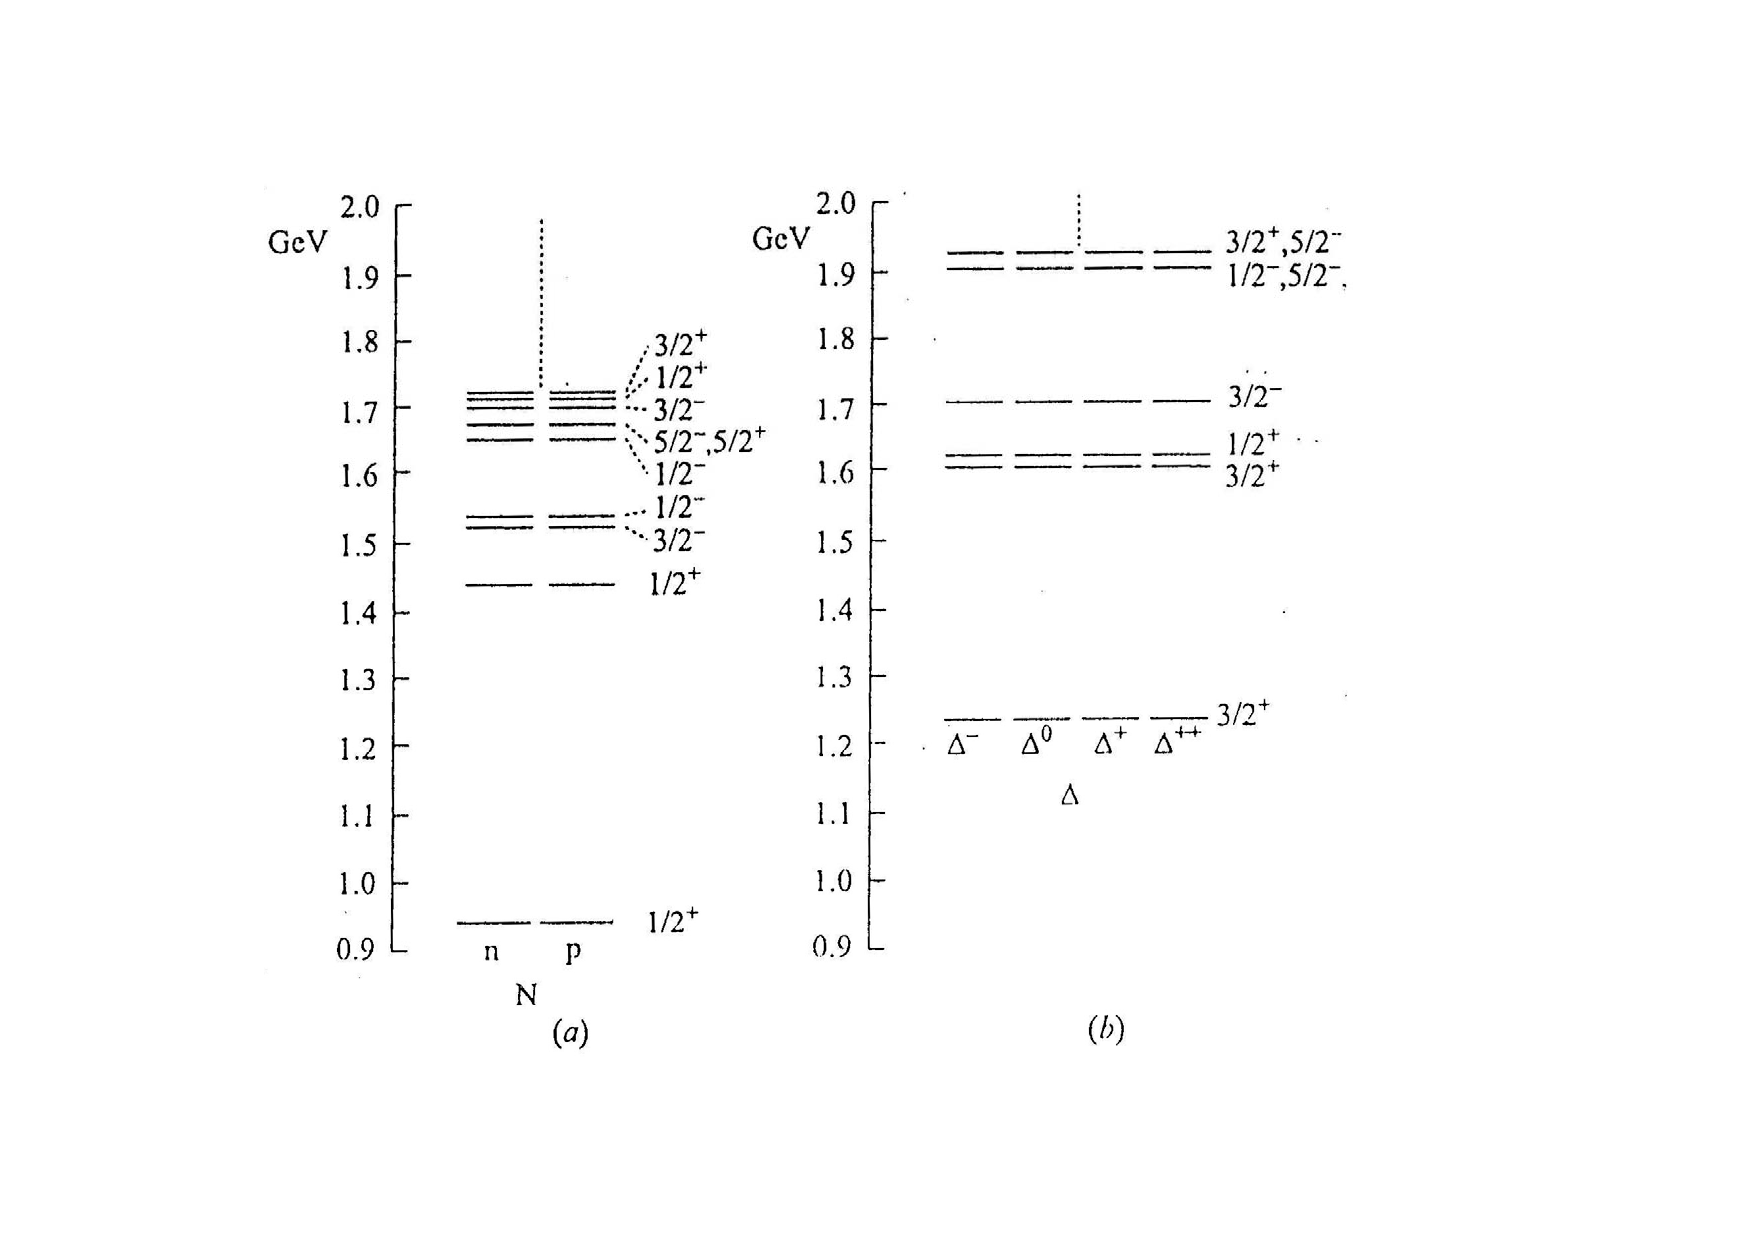
\includegraphics[width=0.8\textwidth]{fig/2-AnregungBaryonen.pdf}
	\caption{Anregungszustände Baryonen. (a) Doublett (N), (b) Quartett
	($\Delta$).}
\end{figure}

Wir haben bereits gesehen, dass es zu jedem Spin $s$, $2s+1$ entartete Zustände
gibt. Für Spin $s=\frac{1}{2}$ gibt es somit zwei Zustände $p^+,n^0$, für
$s=\frac{3}{2}$ vier Zustände, $\Delta^-, \Delta^0, \Delta^+, \Delta^{++}$. Da
für diese Teilchen innere Anregungszustände existieren, können sie nicht
elementar sein und müssen daher aus weiteren Teilchen bestehen,
den \emph{Quarks}.


Quarks müssen als elementare Teilchen, den kleinstmöglichen positiven Spin
$s=\frac{1}{2}$ besitzen.
Angenommen, die uns bekannten Baryonen bestünden nur aus zwei Quarks mit Spin
$s=\frac{1}{2}$, dann wären bei Kopplung von zweien nur Spinwerte von $s=0$
oder $1$ möglich, was nicht unserer Beobachtung entspricht. Die Baryonen müssen
daher aus mindestens drei Quarks bestehen.
Eine geradzahlige größere Anzahl von Quarks wäre
aufgrund der daraus resultierenden geradzaligen Spinwerten nicht möglich.
Eine
größere ungerade Anzahl wie z.b. $5$ wäre möglich, dann müssten
wir aber auch Baryonen mit entsprechendem Spin beobachten, was (noch) nicht der
Fall ist.

Gehen wir also davon aus, dass ein Baryon aus drei Quarks besteht. 
Quarks sind Fermionen, es kann von jeder Sorte nur ein Vertreter
pro Baryon koppeln (Pauli Prinzip). Es muss also mindestens $3$ verschiedene
Quarksorten geben, die für die innere Struktur verantwortlich sind. 

Auffällig ist, dass mehr positiv als negativ geladene Baryonen ($p^+$,
$\Delta^{++}$, $\Delta^+$) existieren, daher ist es wahrscheinlich, dass
mindestens eine Quarksorte eine große positive Ladung besitzt.

Wir wollen nun die Freiheitsgrade der Quarks genauer betrachten. Zunächst 
gibt es zwei Einstellungsmöglichkeiten für die Ladung, nämlich up mit der
Ladung $+\frac{2}{3}$ und down mit der Ladung $-\frac{1}{3}$, weshalb wir von
\emph{Up-} und \emph{Downquarks} sprechen. Diese Einstellungsmöglichkeiten
sind jedoch vom Spin der Quarks selbst unabhängig, ein Upquark hat daher auch
2 Spineinstellungsmöglichkeiten, Spin up und down. Die uns bekannten Baryonen
haben somit die Konfiguration,
\begin{align*}
&n^0 = (u^{\uparrow+\frac{2}{3}},
 	  d^{\uparrow-\frac{1}{3}}, 
	  d^{\downarrow-\frac{1}{3}})\\
&p^+ = (u^{\uparrow+\frac{2}{3}},
 	  u^{\uparrow+\frac{2}{3}}, 
	  d^{\downarrow-\frac{1}{3}})\\
&\Delta^- = (d^{\uparrow-\frac{1}{3}},
 	  d^{\uparrow-\frac{1}{3}},
 	  d^{\uparrow-\frac{1}{3}})\\
&\Delta^0 = (u^{\uparrow+\frac{2}{3}},
 	  d^{\uparrow-\frac{1}{3}},
 	  d^{\uparrow-\frac{1}{3}})\\
&\Delta^+ = (u^{\uparrow+\frac{2}{3}},
 	  u^{\uparrow+\frac{2}{3}},
 	  d^{\uparrow-\frac{1}{3}})\\
&\Delta^{++} = (u^{\uparrow+\frac{2}{3}},
 	  u^{\uparrow+\frac{2}{3}},
 	  u^{\uparrow+\frac{2}{3}}).
\end{align*}
Wir sehen, dass die Teilchenkonfigurationen ohne weitere Freiheitsgrade
nicht möglich sind, da sich maximal zwei Quarks des selben Typs durch ihre
Spineinstellung unterscheiden können. Beim $\Delta^{++}$-Teilchen haben wir
jedoch drei Teilchen des selben Typs, was nach dem Pauli Prinzip verboten wäre.

Es muss also weitere Freiheitsgrade geben und zwar mindestens drei. Wir nennen
diese \emph{Farbladung (color charge)}  $(r,g,b)$ für rot, grün und blau. Die
Farbladung ist die Ladung der starken Wechselwirkung und wird in der
Quantenchromodynamik genauer betrachtet. Wir wollen hier lediglich eine
qualitative Betrachtung durchführen.

\begin{figure}[H]
\centering
\begin{pspicture}(0,-1.47)(3.46,1.47)
\pscircle[linecolor=red](1.69,-1.14){0.33}
\pscircle[linecolor=green](3.13,0.74){0.33}
\pscircle[linecolor=blue](0.33,0.74){0.33}
\pscircle[linecolor=htmlyellow](1.69,1.14){0.33}
\pscircle[linecolor=cyan](3.11,-0.64){0.33}
\pscircle[linecolor=magenta](0.33,-0.64){0.33}
\rput(0.34,0.75){$r$}
\rput(3.13,0.75){$g$}
\rput(1.7,-1.12){$b$}

\rput(3.13,-0.61){$\overline{r}$}
\rput(0.33,-0.61){$\overline{g}$}
\rput(1.7,1.2){$\overline{b}$}
\psline[linewidth=0.04cm](0.54,-0.35)(1.46,0.87)
\psline[linewidth=0.04cm](1.92,0.87)(2.92,-0.33)
\psline[linewidth=0.04cm](0.68,-0.63)(2.76,-0.63)
\psline[linewidth=0.04cm,linestyle=dashed,dash=0.16cm 0.16cm](0.68,0.71)(2.78,0.71)
\psline[linewidth=0.04cm,linestyle=dashed,dash=0.16cm 0.16cm](0.52,0.45)(1.5,-0.85)
\psline[linewidth=0.04cm,linestyle=dashed,dash=0.16cm 0.16cm](1.88,-0.85)(2.92,0.47)
\end{pspicture}
\caption{Farbladungen und Antifarbladungen.}
\end{figure}

In der Elektrostatik kann man die Ladungskonjugation als Punktspiegelung
auffassen. Bei den Farbladungen existiert z.B. für rot ein
\oline{rot}, das Gegenteil von rot, es entspricht aber weder grün
oder blau. Für die Ladungskonjugation gilt daher,
\begin{align*}
\begin{pmatrix}
r \\ g \\ b
\end{pmatrix}
\overset{\hat{C}}{\mapsto}
\begin{pmatrix}
\overline{r} \\ \overline{g} \\ \overline{b}
\end{pmatrix}.
\end{align*}
Die für uns beobachtbaren Teilchen (Baryonen) sind jedoch farblos, d.h.
Baryonen eines Typs sind nicht unterscheidbar und wechselwirken nicht direkt
(d.h. in 1. Ordnung) durch den Mechanismus der Quarkwechselwirkungen.
\begin{bspn} Mögliche Konfiguration eines $\Delta^{++}$,
\begin{align*}
\Delta^{++} = (u^{\uparrow+\frac{2}{3}g},
 	  u^{\uparrow+\frac{2}{3}r},
 	  u^{\uparrow+\frac{2}{3}b})\bsphere
\end{align*}
\end{bspn}
\begin{bspn}
Es ist aber auch möglich, ein rot und ein \oline{rot} zusammenzubringen,
wodurch ein fabloses Teilchen, ein \emph{Meson} entsteht.
\begin{align*}
\pi^0 = (u^{r}\overline{u}^{\overline{r}}).
\end{align*}
Mesonen bestehen aus zwei Quarks. Aufgrund der Ladungen sind somit auch
Triplets möglich. Da Mesonen aus Quarks und Antiquarks bestehen haben sie eine
sehr endliche Lebensdauer ($\pi^0$ von $2.6\cdot 10^{-8}s$).\bsphere
\end{bspn}

Die Farbladungen führen zu Wechselwirkungen zwischen den Quarks. Wir können
diese Wechselwirkung durch das Modelpotential,
\begin{align*}
V(r) = -\frac{\alpha_s}{r} + Ar
\end{align*}
beschreiben.

Im Gegensatz zum Coulomb-Potential bei dem ein Teilchen durch das Aufbringen
von endlich viel Energie unendlich weit vom Potentialmittelpunkt entfernt
werden kann, nimmt hier das Potential mit wachsendem Abstand linear zu.
Beim Versuch Farbladungen zu trennen, entstehen neue farblose Mesonen, wenn die
Wechselwirkungsenergie größer wird als die Ruhemasse des Mesons.

\sfigure[!htpb]%
	{2-MesonenTrennung.pdf}%
	{\KuckukKern, S. 188}%
	{Zum Blasenmodell der Hadronen (Bag Modell).}

Insgesamt ist so weniger Energie notwendig als für die Trennung der einzelnen
Farbladungen. Als Konsequenz sehen wir, dass es nur farblose Teilchen als
beobachtbare Teilchen auftreten.

Es handelt sich hier lediglich um eine stark vereinfachte Modellvorstellung,
die schnell an ihre Grenzen stößt. In Wirklichkeit ist die Wechselwirkung
deutlich komplizierter, eine detailierte Behandlung ist aber für unsere
Fragestellung nicht zweckmäßig und sprengt den Rahmen der Vorlesung.

Wir wollen nun zur Kernphysik zurückkehren und die Frage klären, warum auch
farblose Teilchen wie $p^+, n^0$ eine attraktive Wechselwirkung erfahren.
Aufgrund der Ladung lässt sich eine Coulomb-Wechselwirkung sofort ausschließen.
Erinnern wir uns zunächst an die Van-Der-Waals Wechselwirkung. Hier induzieren
Atome durch fluktuierende Ladungsverschiebung in anderen Atomen Dipolmomente,
wodurch eine Attraktion zwischen den Atomen stattfindet. Ähnlich induzieren
auch fluktuierende Farbladungsverschiebungen, Farbladungsverschiebungen in
anderen Teilchen, wodurch diese ebenfalls eine attraktive Wechselwirkung
erfahren. Diese Wechselwirkung ist als Induktionsprozess 2. Ordnung 
schwächer als die Wechselwirkung zwischen den Farbladungen selbst; bei
den im Atom vorliegenden Längenskalen jedoch deutlich stärker als beispielsweise
die Coulomb Wechselwirkung für gleichnamige Teilchen.

Wir wollen diese Wechselwirkung nun für den konkreten Fall der
Proton-Neutron-Wechselwirkung betrachten. Durch den Induktionsprozess werden
hier $\pi^+$-Mesonen, farblose Teilchen, die aus einem Up-Quark
und einem Anti-Down-Quark bestehen, ausgetauscht.
 \begin{figure}[!htbp]
\centering
\begin{pspicture}(0,-0.8)(3.76,1)
\pscircle(0.59,-0.2028125){0.59}
\pscircle(3.17,-0.2028125){0.59}

\rput[b](0.32953125,-0.1){\color{gdarkgray}u}
\rput[b](0.8095313,-0.1){\color{gdarkgray}u}
\rput(0.56453127,-0.5){\color{gdarkgray}d}

\rput[b](2.9095314,-0.1){\color{gdarkgray}u}
\rput[b](3.3845313,-0.1){\color{gdarkgray}d}
\rput[b](3.1445312,-0.5){\color{gdarkgray}d}

\psline[linecolor=darkblue]{<->}(1.22,-0.1528125)(2.52,-0.1528125)

\rput(0.6045312,0.7371875){\color{gdarkgray}$p^+$}
\rput(3.188125,0.7371875){\color{gdarkgray}$n^0$}
\rput(1.9445312,0.2171875){\color{gdarkgray}$\pi^+$}
\end{pspicture} 
\qquad
\begin{pspicture}(0,-2.2)(3.26,2.3)
\psellipse(0.42,0.995625)(0.4,0.78)

\psellipse(2.86,0.995625)(0.4,0.78)

\psellipse(0.4,-0.984375)(0.4,0.78)


\psellipse(2.86,-0.984375)(0.4,0.78)

\psline(0.9,1.515625)(2.4,1.515625)
\psline(0.92,1.015625)(2.4,1.015625)
\psline(0.92,-0.964375)(2.4,-0.964375)
\psline(0.92,-1.364375)(2.4,-1.364375)

\psline[linecolor=yellow]{->}(2.4,0.575625)(1.94,0.575625)(1.36,-0.5)(0.92,-0.5)
\psline[linecolor=darkblue]{->}(0.92,0.595625)(1.38,0.595625)(1.96,-0.5)(2.4,-0.5)

\psellipse(1.65,0.075625)(0.55,0.3)


\rput[b](0.4,1.4){\color{gdarkgray}d}
\rput[b](0.4,0.95){\color{gdarkgray}u}
\rput[b](0.4,0.5){\color{gdarkgray}u}

\rput[b](2.85,1.4){\color{gdarkgray}d}
\rput[b](2.85,0.95){\color{gdarkgray}u}
\rput[b](2.85,0.5){\color{gdarkgray}d}

\rput[b](0.4,-0.6){\color{gdarkgray}d}
\rput[b](0.4,-1.05){\color{gdarkgray}u}
\rput[b](0.4,-1.5){\color{gdarkgray}d}

\rput[b](2.85,-0.6){\color{gdarkgray}u}
\rput[b](2.85,-1.05){\color{gdarkgray}u}
\rput[b](2.85,-1.5){\color{gdarkgray}d}

\rput[b](1.9695313,-0.05){\color{gdarkgray}u}
\rput[b](1.3445313,-0.05){\color{gdarkgray}\oline{d}}

\rput[b](0.4,2){\color{gdarkgray}$p^+$}

\rput[b](2.85,2){\color{gdarkgray}$n^0$}

\rput[b](0.4,-2.1){\color{gdarkgray}$n^0$}

\rput[b](2.85,-2.1){\color{gdarkgray}$p^+$}
\end{pspicture} 
\caption{Rolle des $\pi^+$-Meson bei der Proton-Neutron Wechselwirkung.}
\end{figure}

Um diese Wechselwirkung mit anderen uns bekannten zu vergleichen, müssen wir
die Wechselwirkungteilchen vergleichen. Die Elektromagnetische Wechselwirkung
basiert beispielsweise auf Photonen, die keine Ruhemasse und daher unendliche
Reichweite haben. Die Mesonen dagegen besitzen eine Ruhemasse und haben daher
nur eine endliche Reichweite. Mithilfe der Energie-Masse-Äquivalenz und der
Heisenbergschen Unschärferelation können wir die Reichweite abschätzen. Gehen wir von
\begin{align*}
\Delta t = \frac{\hbar}{\Delta E}
\end{align*} 
aus, wobei $\Delta E \ge m_{\pi}c^2$, so erhalten wir für die Reichweite,
\begin{align*}
R = c\Delta t = \frac{c\hbar}{\Delta E} \le \frac{\hbar}{cm_\pi}.
\end{align*}
Für $\pi$-Mesonen mit $m_\pi = 140 \frac{\mathrm{MeV}}{c^2}$ ergibt sich der
Wert,
\begin{align*}
R \le 1.4\mathrm{fm}.
\end{align*}
 \begin{figure}[!htbp]
\centering
\begin{pspicture}(0,-1.3425)(4.8096876,1.3225)

\psbezier[linecolor=darkblue](0.5046875,-0.9175)(1.1446875,-0.2175)(1.1046875,0.6825)(0.6468304,1.3025)
\psbezier[linecolor=yellow](3.8646874,-0.9175)(3.2246876,-0.2175)(3.2646875,0.6825)(3.7225447,1.3025)

\pscircle[fillstyle=solid,fillcolor=glightgray](0.7746875,-0.5275){0.19}
\pscircle[fillstyle=solid,fillcolor=glightgray](3.4746876,-0.3075){0.19}
\psline(0.6646875,1.0425)(0.8846875,1.1825)
\psline(0.8446875,0.3025)(1.1246876,0.3025)

\psline[linestyle=dotted,dotsep=0.06cm]{->}(1.1046875,0.3625)(3.3846874,0.9425)
\psdots(3.5246875,0.9625)

\rput(0.735,-1.1875){\color{gdarkgray}Nukleon 1}
\rput(4.0295315,-1.1875){\color{gdarkgray}Nukleon 2}
\rput(0.5565625,0.6725){\color{gdarkgray}$\Delta x$}
\rput(2.2190626,0.3925){\color{gdarkgray}$\Delta t$}
\end{pspicture} 
\caption{Reichweite der Wechselwirkung.}
\end{figure}

Aufgrund unserer stark vereinfachten Modellvorstellung ist dieses Vorgehen nur
ein zur groben Abschätzung der Reichweite zulässiges Mittel.

Wir sehen also, dass die 2. Ordnung Farbwechselwirkung, die durch den Austausch
von $\pi$-Mesonen stattfindet, eine Reichweite von ungefähr Kerndurchmesser
hat. Die Teilchen im Kern wechselwirken also hauptsächlich untereinander. Damit
sie mit Teilchen in anderen Kernen
wechselwirken, müsste man die Kerne auf einen Abstand kleiner als der
Kerndurchmesser zusammenbringen.\footnote{Dies ist eine große Herausforderung
beim Bau von Fusionsreaktoren.}

\sfigure[htpb][1]%
	{2-TheQuarks.pdf}%
	{\TiplerMPFife, S. 569}%
	{Quarks.}
	
\sfigure[htpb][1]%
	{2-TheLeptons.pdf}%
	{\TiplerMPFife, S. 569}%
	{Leptonen.}

\subsection{Kernmassenbestimmung und Kernmodelle} 

Wir wollen nun die Bindungsenergie der 2. Ordnung Farbladungswechselwirkung
untersuchen. Es stellt sich natürlich die Frage, wie man diese überhaupt messen
kann. Die Energie Masse Äquivalenz $E=mc^2$ besagt, dass die Information über
die  Bindungsenergie bereits in der Masse enthalten ist. Eine Änderung der
Bindungsenergie führt somit zu einer Änderung der Masse. Misst man nun die
Masse der einzelnen Nukleonen und anschließend die der Atome, kann man aus der
Differenz der Massen die Größe der Bindungsenergien berechnen.

\begin{figure}[!htbp]
	\centering
	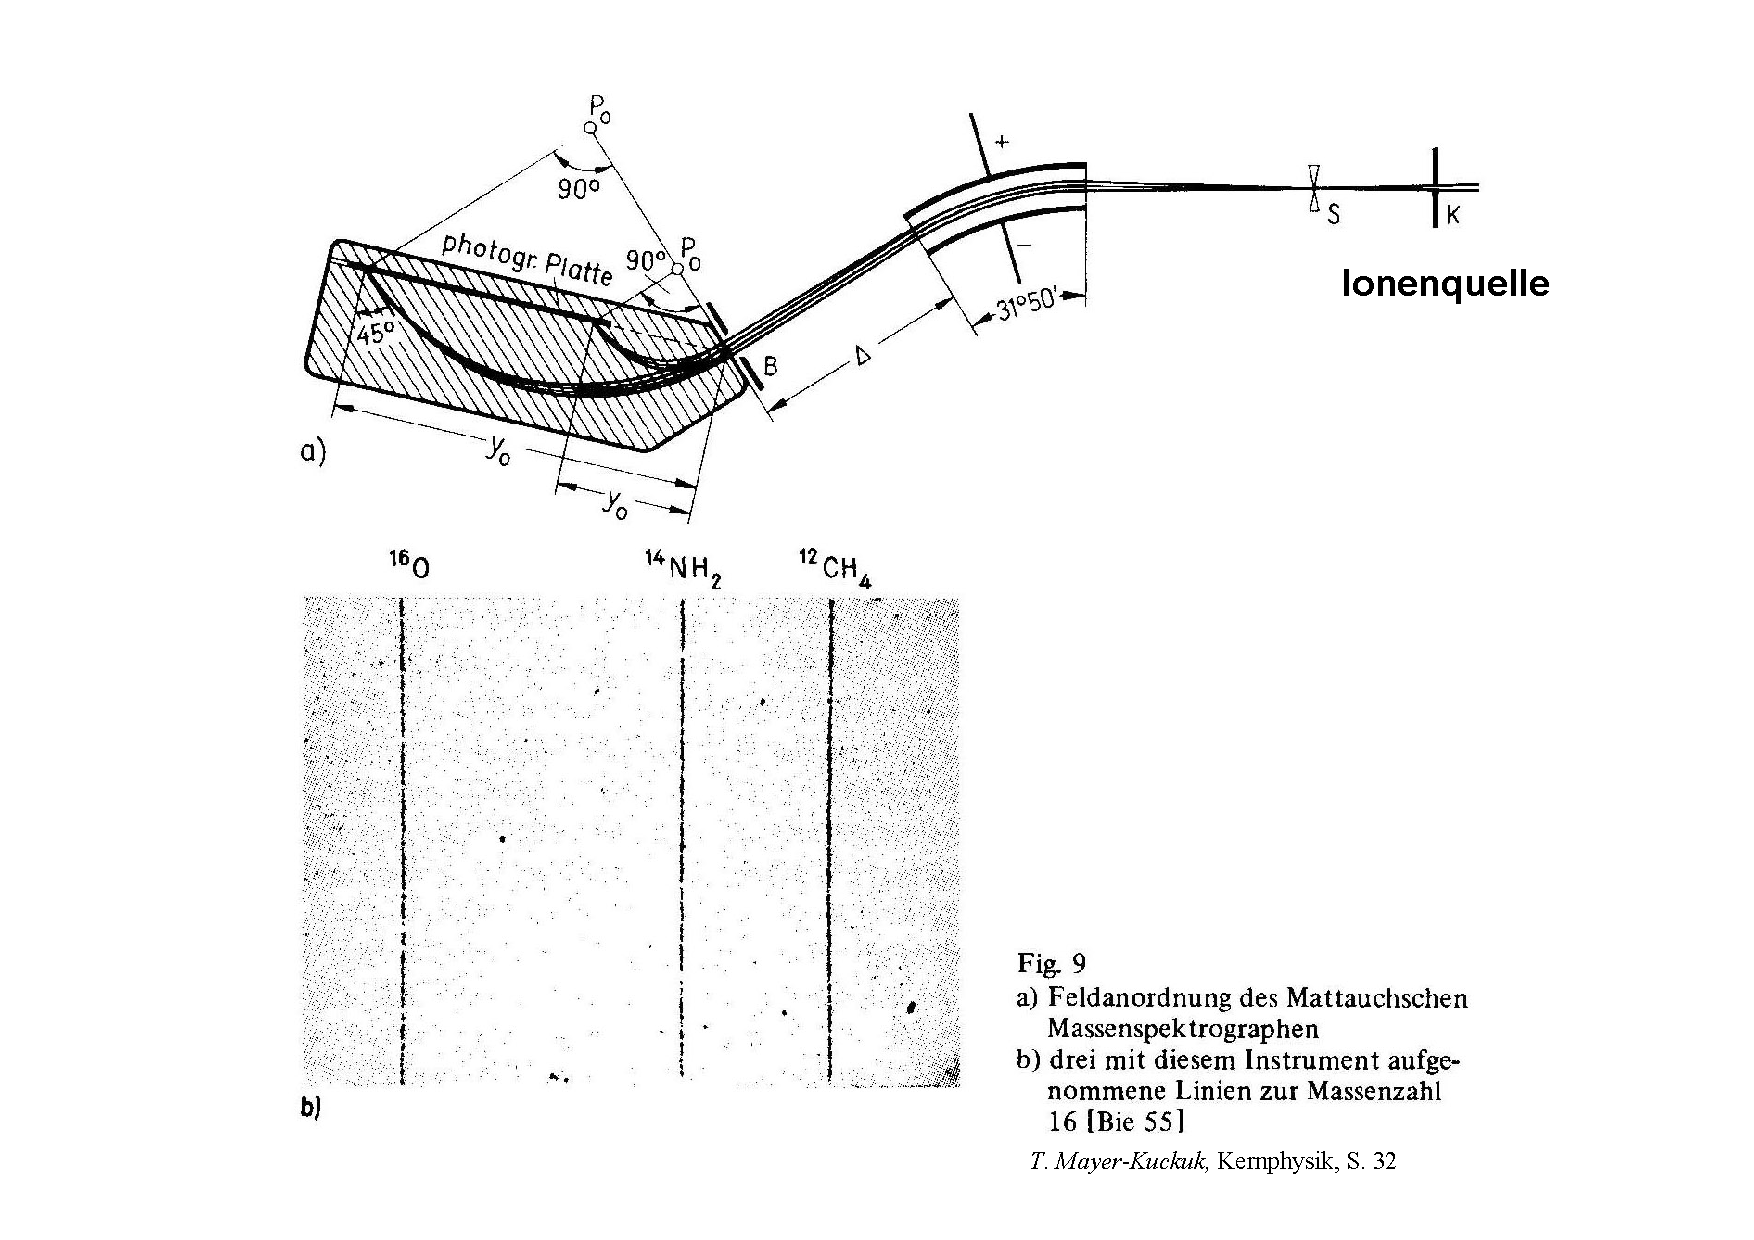
\includegraphics[width=0.8\textwidth]{fig/2-Massenspektrograph.pdf}
\end{figure}

\begin{defnn}
Die \emph{Bindungsenergie} ist eine positive Größe, gegeben durch
\begin{align*}
B(Z,N) = \left[Zm_{p^+} + Nm_{n^0} - m(Z,N) \right]c^2,
\end{align*}
wobei $Z$ die Anzahl der Protonen, $N$ die Anzahl der Neutronen und $m(Z,N)$
die reale Masse eines Kerns mit $N$ und $Z$ bezeichnet.\fishhere
\end{defnn}
\begin{bspn} Masse des
Protons, Neutrons und Elektrons
\begin{align*}
m_{p^+} = 938.3\frac{\mathrm{MeV}}{c^2},\quad m_{n^0} =
939.6\frac{\mathrm{MeV}}{c^2},\quad m_{e^-} = 0.591\frac{\mathrm{MeV}}{c^2}.
\end{align*}
Die Elektronenmasse ist also vernachlässigbar gegenüber der der
Protonen und Neutronen.\bsphere
\end{bspn}
\begin{bspn}
Die Atomare Masseneinheit
\begin{align*}
1u = \frac{1}{12}m\left({}^{12}C\right) = 931.5\frac{\mathrm{MeV}}{c^2} \entspr
1.6606\cdot 10^{-24}\mathrm{g},
\end{align*}
ist kleiner als die Summe der einzelnen Protonen- und Neutronenmassen im
${}^{12}C$, es fehlt also bereits die ${}^{12}C$-Bindungsenergie.\bsphere
\end{bspn}
\begin{bspn}
Die Messgenauigkeit der Massenspektrometrie heute $\dfrac{\Delta m}{m} \approx
10^{-10}$.\bsphere
\end{bspn}

\sfigure%
	{2-BindungsEnergieProNukleon.pdf}
	{\KuckukKern, S. 36}
	{Zentrales Ergebnis der Massenspektroskopie: Bindungsenergie pro Nukleon als
	Funktion von $A$ für stabile Kerne.}

Wollen wir Atome vergleichen, benötigen wir noch einige Begriffe. 

\begin{figure}[!ht]
  \centering
  \begin{pspicture}(-2.6,-1.2)(5,1.2)

\psbezier{->}(2.9721875,0.7107813)(2.4521875,-0.08921875)(2.4321876,1.0707812)(1.8121876,0.41078126)
\psbezier{<-}(1.9574513,0.014663258)(2.5974512,-0.44533673)(1.8574514,-0.68533677)(2.4574516,-0.9253368)
\psbezier{->}(0.3121875,0.45078126)(0.8321875,-0.12921876)(0.8521875,1.0307813)(1.3321875,0.45078126)
\psbezier{<-}(1.2471875,0.008774293)(0.4871875,0.008774293)(1.0671875,-0.6712257)(0.4071875,-0.5712257)

\rput(1.6289062,0.20578125){\color{darkblue}\Large ${}_Z^AX_N$}

\rput[l](2,0.9607813){\color{gdarkgray}chemisches Element}
\rput[l](2.6,-0.9792187){\color{gdarkgray}Neutronenzahl}
\rput[r](0.7,0.6407812){\color{gdarkgray}Gesamtnukleonenzahl}

\rput[r](0.6,-0.3){\color{gdarkgray}Kernladungszahl}
\end{pspicture} 
  \caption{Notation eines chemischen Elements $X$ mit Kernladungszahl $Z$,
  Neutronenzahl $N$ und Gesamtnukleonenzahl $A$.}
\end{figure}

\begin{defnn}
\emph{Isotope} sind Kerne mit gleicher Kernladungszahl $Z$ aber
unterschiedlicher Neutronenzahl $N$ und demnach unterschiedlicher Massenzahlen $A$.
\begin{bspn}
${}^{12}C$, ${}^{13}C$ und ${}^{14}C$.\bsphere
\end{bspn}
\emph{Isobare} sind Kerne mit derselben Massenzahl $A$, jedoch mit
unterschiedlicher Neutronenzahl $N$ und deshalb auch unterschiedlicher Kernladungszahl $Z$.
\begin{bspn}
${}^{12}C$, ${}^{12}N$ und ${}^{12}B$.\bsphere
\end{bspn}
\emph{Isotone} sind Kerne mit derselben Neutronenzahl $N$, aber mit
unterschiedlicher Massenzahl $A$ und deshalb auch unterschiedlicher
Kernladungszahl $Z$.
\begin{bspn}
${}^{12}C$, ${}^{13}N$ und ${}^{14}O$.\bsphere\fishhere
\end{bspn}
\end{defnn}

\begin{figure}[!htbp]
\centering
\begin{pspicture}(0,-1.2910937)(4.845,1.2910937)

\psline{->}(0.32,-1.1076914)(0.32,1.1726646)
\psline{->}(0.2753125,-1.07)(4.2353125,-1.07)
\psline[linecolor=darkblue](0.8553125,0.8726562)(3.6553125,-0.72734374)
\psline[linecolor=yellow](0.8553125,0.07320729)(3.6553125,0.07320729)
\psline(2.2553124,-0.72734374)(2.2553124,0.8726562)

\rput(2.325625,1.1226562){\color{gdarkgray}Isotone}

\rput(3.935625,0.36265624){\color{gdarkgray}Isotope}

\rput(4.275625,-0.75734377){\color{gdarkgray}Isobare}

\rput(4.405156,-1.1373438){\color{gdarkgray}$N$}

\rput(0.09796875,1.0826563){\color{gdarkgray}$Z$}
\end{pspicture} 
\caption{Isotone, Isotope und Isobare.}
\end{figure}

\begin{bemn}[Beobachtungen.]
\begin{enumerate}[label=\arabic{*}.)]
\item Die Bindungsenergie pro Nukelon $\frac{B}{A}$ hat ein Maximum bei $A\sim
60$. Wir können daher durch Spaltung von schweren bzw. Fusion von leichten
Kernen Energie gewinnen. Durch Fusion der leichtesten Kerne können über
$\approx 4\mathrm{MeV}$ frei werden, während wir durch Spaltung der schwersten
Kerne lediglich $\approx 1\mathrm{MeV}$ erhalten.
\item Leichte Kerne zeigen eine ``Schalenstruktur''.
\item Größenordnungsmäßig bleibt $\frac{B}{A}$ für schwere Kerne nahezu
konstant. Die Wechselwirkung eines Nukleons betrifft nur seine nächsten
Nachbarn, die weiteren Nukleonen im Kern spielen keine Rolle. Andernfalls würden
$A-1$ Bindungspartner auch $\frac{A(A-1)}{2}$ Bindungen erzeugen und $\frac{B}{A}$
wäre proportional zu $A$.
\end{enumerate}
\end{bemn}

Wir können diese Eigenschaften sehr gut mittels einem Tröpfchenmodell
beschreiben. In einem Tropfen herrscht unabhängig von der Größe des Tropfens
stets die selbe Dichte. Dies entspricht den Ergebnissen der Streuexperimente,
die eine nahezu homogene Ladungsverteilung für schwere Teilchen besagen. Ein
Teilchen in einem Tropfen wechselwirkt nur mit seinen nächsten Nachbarn. Die
Wechselwirkung ist von der Größe des Topfens unabhängig.

Das Tröpfchenmodell scheitert jedoch beim Übergang zu $<10$ Nukleonen und der
hier vorliegenden Schalenstruktur. In diesem Fall lassen sich die Teilchen als
nahezu ideales Gas interpretieren und durch das Modell des freien Teilchens
beschreiben.

Zur Lösung wählen wir als effektives Model ein Fermigas im
mittleren Potential. Innerhalb des Kastenpotentials kann sich ein Teilchen
frei bewegen, während am Rand viel Energie notwendig ist, um es vom Verband zu
lösen. Die Physik in diesem Potential wird durch das Pauli-Prinzip dominiert,
welches bestimmt wie oft ein Energiezustand überhaupt auftreten kann.

Wir werden sehen, dass die Energie dieses Potentials viel größer ist als die
Bindungsenergie pro Nukleon $E_\text{Fermi}>>\frac{B}{A}$.
\begin{bspn}
$E_\text{Fermi}\approx40\mathrm{MeV}$, $\dfrac{B}{A}\approx
8\mathrm{MeV}$.\bsphere
\end{bspn}
\begin{figure}[!ht]
  \centering
\begin{pspicture}(-0.25,-0.74717915)(2.42,0.7266349)

\psline(0,0.7066349)(0.7,0.7066349)(0.7,-0.6733651)(1.7,-0.6733651)(1.7,0.7066349)(2.4,0.7066349)
\psline(0.8,-0.32)(1.6,-0.32)
\psline(0.8,-0.023)(1.6,-0.023)
\psline[linecolor=darkblue](0.8,0.25)(1.6,0.25)

\pscircle[fillstyle=solid,fillcolor=white](0.91,0.25){0.09}
\pscircle[fillstyle=solid,fillcolor=white](0.91,-0.023){0.09}
\pscircle[fillstyle=solid,fillcolor=white](0.91,-0.32){0.09}

\pscircle[fillstyle=solid,fillcolor=white](1.49,0.25){0.09}
\pscircle[fillstyle=solid,fillcolor=white](1.49,-0.023){0.09}
\pscircle[fillstyle=solid,fillcolor=white](1.49,-0.323){0.09}

\rput[r](0.6,0.25663492){\color{gdarkgray}$E_\text{Fermi}$}
%\rput{90}(2.020937,1.8641888)
%{\rput(1.9125,-0.063365094){\color{gdarkgray}Zustände}}
\end{pspicture} 
  \caption{Kastenpotential mit diskreten Energiezuständen.}
\end{figure}

\subsubsection{Ideales Fermigas im Kastenpotential}

Die Wechselwirkung der Fermionen untereinander ist sehr klein im Verhältnis zur
Fermienergie, weshalb wir diese in unserem Modell vernachlässigen wollen.
Da Messungen außerdem zeigen, dass die Dichteverteilung nahezu konstant
ist, gehen wir davon aus, dass außer den elementaren keine weiteren Kräfte
wirken.

Wir wollen nun die quantenmechanischen Zustände im 3-dimensionalen
Kastenpotential untersuchen. Dazu wählen wir für die Nukleonen als effektives
Potential,
\begin{align*}
V(r) =
\begin{cases}
0 & r > a,\\
-V_0 & r\le a,
\end{cases}
\end{align*}
wobei $a$ den Kernradius bezeichnet.

Um unsere Rechnungen zu vereinfachen, gehen wir davon aus, dass der Kern
Würfelform mit Kantenlänge $a$ hat. Dadurch kommt in unserem
Modell lediglich ein Vorfaktor der Größenordnung $1$ dazukommt. Durch die
Würfelform können wir die 3-dimensionale Schrödingergleichung in drei
1-dimensionale separieren. Die Gesamtwellenfunktion ist somit gegeben durch,
\begin{align*}
\Psi_\text{ges} = \Psi_x\Psi_y\Psi_z,
\end{align*}
mit der Gesamtenergie,
\begin{align*}
E_\text{ges} = E_x + E_y + E_z.
\end{align*}

Wir fordern weiterhin, dass am ``Potentialrand'' Knotenpunkte vorliegen, also
die Amplitude dort verschwindet. Die Lösungen der SGL sind stehende Wellen
der Form,
\begin{align*}
\Psi_x = \frac{2}{\sqrt{2}a}\begin{cases}
\cos k_x x, & k_x = \frac{\pi \lambda}{a},  \lambda=1,3,5,\ldots\\
\sin k_x x, & k_x = \frac{\pi \lambda}{a},  \lambda=2,4,6,\ldots 
\end{cases}
\end{align*}
$\lambda$ ist hier Quantenzahl.

Entsprechend ergibt sich für die Energie die Form,
\begin{align*}
&E_x^{(\lambda)} = \frac{\hbar^2}{2m}\left(k_x^{(\lambda)}\right)^2 =
\frac{1}{2m}\left(\frac{\pi\hbar}{a}\lambda_x\right)^2.
\end{align*}
Die Gesamtenergie eines Teilchens, das durch die Zustände $\lambda_x,\lambda_y$
und $\lambda_z$ charakterisiert wird, ist somit gegeben durch,
\begin{align*}
&E_\text{ges} =
\frac{1}{2m}\left(\frac{\pi\hbar}{a}\right)^2\underbrace{\left(\lambda_x^2 +
\lambda_y^2+ \lambda_z^2\right)}_{:=\rho^2}.
\end{align*}

Wir wollen nun untersuchen, wie sich unser Modell verhält, wenn wir viele
Fermionen in das Potential einbringen. Die Fermionen haben lediglich vier
unterscheidbare Konfigurationen nämlich Proton/Neutron und Spin Up/Down. Das
Pauliprinzip besagt daher, dass pro Energiezustand nur zwei Nukleonen eines Typs
möglich sind.

\begin{figure}[!ht]
  \centering
\begin{pspicture}(0,-0.7041111)(2.4512014,0.7041111)
\psline(0.0,0.69)(0.7,0.69)(0.7,-0.69)(1.7,-0.69)(1.7,0.69)(2.4,0.69)
\psline(1.04,-0.37588888)(1.36,-0.37588888)
\psline(1.04,0.124111116)(1.36,0.124111116)
\psline(0.8,0.55)(1.6,0.55)
\pscircle(0.91,0.120000005){0.09}
\pscircle(0.91,-0.38){0.09}
\pscircle(1.49,-0.38){0.09}
\pscircle(1.49,0.120000005){0.09}
\psline[linecolor=darkblue]{->}(0.91,-0.035888884)(0.91,0.36411113)
\psline[linecolor=darkblue]{->}(1.49,-0.5358889)(1.49,-0.13588889)
\psline[linecolor=yellow]{<-}(0.91,-0.6358889)(0.91,-0.23588888)
\psline[linecolor=yellow]{<-}(1.49,-0.13588889)(1.49,0.2641111)
\psline(1.75,0.124111116)(2,0.124111116)

\rput(2.2047951,0.094111115){\color{gdarkgray}$E_F$}
\end{pspicture} 
  \caption{Fermipotential mit 4 Nukleonen mit Spin Up/Down.}
\end{figure}

Somit erhalten wir eine neue Energieskala. Die \emph{Fermienergie} $E_F$ ist
die Energie, bis zu der von $n$ Teilchen alle Zustände besetzt sind. Wenn wir
$E_F$ berechnen wollen, müssen wir also Zustände ``zählen''. Dazu führen wir
die \emph{Zustandsdichte} $\dfrac{\dn}{\dE}$ ein, die die Anzahl der
Energiezustände pro Energieintervall beschreibt.
%TODO: 3d Bild Energiezustände.
Betrachten wir eine Kugel mit Radius $\rho$ im Zustandsraum, so gilt
\begin{align*}
\dn = \frac{1}{8}4\pi \rho^2\drho.
\end{align*}
Der Faktor $\frac{1}{8}$ entsteht, da wir nur den rechten oberen Quadranten
betrachten, $\lambda_x,\lambda_y,\lambda_z > 0$. Verwenden wir nun die
$\rho$-Impuls Beziehung,
\begin{align*}
\rho = \frac{ap}{\pi\hbar},
\end{align*}
so erhalten wir
\begin{align*}
&\dn = \frac{1}{8}4\pi \frac{a^2p^2}{\pi^2\hbar^2}\frac{a}{\pi\hbar}\ddp
= \frac{1}{2\pi^2\hbar^3}\underbrace{a^3}_{:=V}p^2\ddp.\tag{*}
\end{align*}
Die Energie-Impuls Beziehung $p^2 = 2mE$ liefert,
\begin{align*}
&\frac{\ddp}{\dE} = \frac{\diffd\sqrt{2mE}}{\dE} = \frac{m}{\sqrt{2mE}},\\
\Rightarrow\;& p^2\ddp = 2mE \frac{m}{\sqrt{2mE}}\dE = m^{3/2}\sqrt{2E}\dE
\end{align*}
Setzen wir dies in (*) ein, erhalten wir die Zustandsdichte,
\begin{align*}
\frac{\dn}{\dE} = \frac{m^{3/2}}{\sqrt{2}\pi^2\hbar^3}V\sqrt{E}
\end{align*}

\begin{figure}[!ht]
  \centering
\begin{pspicture}(-0.5,-1)(4.5,2.5)
\psaxes[labels=none,ticks=none]{->}%
 (0,0)(-0.2,-0.2)(4,2)[\color{gdarkgray}$E$,-90][\color{gdarkgray}$\frac{\dn}{\dE}$,0]

 \psline(3,0)(3,1.72)

 \psplot[linewidth=1.2pt,%
	     linecolor=darkblue,%
	     algebraic=true]%
	     {0}{3.5}{x^0.5}
 	     
 \psxTick(3){\color{gdarkgray}E_F}
 
 \rput(2,1.8){\color{gdarkgray}$\sim\sqrt{E}$}
\end{pspicture} 
  \caption{Integration der Zustandsdichte.}
\end{figure}

Für einen Kern mit $n$ Spin $\frac{1}{2}$-Teilchen gleichen Typs kann jeder
Energiezustand doppelt besetzt werden. Die Anzahl der Energiezustände ist daher,
\begin{align*}
n &= 2\int\limits_{0}^{E_F} \frac{\dn}{\dE}\dE =
2\frac{m^{3/2}V}{\sqrt{2}\pi^2\hbar^3}\int\limits_{0}^{E_F} \sqrt{E}\dE
= \frac{2^{3/2}}{3}\frac{m^{3/2}V}{\pi^2\hbar^{3}}E_F^{3/2}\\
\Rightarrow E_F &=
\left(\frac{3}{2^{3/2}}\frac{\pi^2\hbar^3}{m^{3/2}V}n\right)^{2/3}
= \frac{3^{2/3}}{2}\frac{\pi^{4/3}\hbar^2}{m}\left(\frac{n}{V}\right)^{2/3}
\end{align*}
Unsere vereinfachte Modellvorstellung erlaubt es nicht, den Wert exakt
auszurechnen, festzuhalten ist jedoch, dass 
die Fermieenergie proportional zur $(\text{Kerndichte})^{2/3}$ ist.

Mit der gemessenen Kerndichte erhalten wir für die Fermienergie,
\begin{align*}
E_F = 30\mathrm{MeV}.
\end{align*}
Insgesamt verfügen wir nun über zwei Energieskalen. Zum einen die Fermienergei
$\im 30\mathrm{MeV}$ und zum anderen die Bindungsenergie $8\mathrm{MeV}$.

\begin{figure}[!ht]
  \centering
\begin{pspicture}(0,-0.82705563)(2.4141111,0.8270556)
\psline(0.0,0.8129445)(0.7,0.8129445)(0.7,-0.8129445)(1.7,-0.8129445)(1.7,0.8129445)(2.4,0.8129445)
\psline[linecolor=darkblue](0.8,0.23294444)(1.6,0.23294444)
\psline{<->}(1.7858889,-0.79294443)(1.7858889,0.20705555)
\psline{<->}(1.7858889,0.24705556)(1.7858889,0.7670556)
\rput(2.1447952,-0.18294445){\color{gdarkgray}$E_F$}
\rput(2.0530765,0.53705555){\color{gdarkgray}$B$}
\end{pspicture} 
  \caption{Bindungs- und Fermieenergie im Fermipotential.}
\end{figure}

\begin{bemn}[Bemerkungen.]
\begin{enumerate}[label=\arabic{*}.]
  \item 
Später werden wir in der Festkörperphysik ein analoges Modell entwickeln.
Betrachten wir die Elektronen im Kupferatom, so sind dies auch Fermionen, die
man durch ein Fermipotential beschreiben kann. Die Bindungsenergie entspricht
dann der Austrittsenergie der Elektronen. Diese beträgt lediglich $\sim
3\mathrm{eV}$ gegenüber der Fermienergie $\sim 7\mathrm{eV}$. 
\item
Unsere bisherigen Überlegungen gelten nur für nicht wechselwirkende Teilchen
bei $T=0$. Für thermische Energien $k_BT<<E_F$ und $E_B<<E_F$ verhält sich der
Kern aber näherungsweise wie ein ideales, d.h. wechselwirkungsfreies, Fermigas.
\item
Während die Neutronen neutral bezüglich der Coulomb-Wechselwirkung sind,
besitzen die Protonen eine positive Ladung. Das Coulombpotential verhält sich
wie $\dfrac{1}{r}$, weshalb Protonen beim Einbringen in den Kern bereits ein
höheres Energieniveau als Neutronen haben. Protonen und Neutronen streben
danach das Energieniveau in Balance, d.h. die Fermienergie auf dem gleichen
Niveau zu halten. Sind ``zu viele'' Neutronen im Kern, beobachten wir
$\beta^-$-Zerfall,
\begin{align*}
n^0 \longrightarrow p^+ + e^- + \overline{\nu}_e. 
\end{align*}
Sind dagegen zu viele Protonen im Kern, findet $\beta^+$-Zerfall statt,
\begin{align*}
p^+ \longrightarrow n^0 + e^+ + \nu_e.
\end{align*}
$\beta$-Zerfälle finden so lange statt, bis die $p^+$ und $n^0$ Niveaus bis zur
gleichen Fermienergie gefüllt sind und so ein stabiler Zustand erreicht ist.
\begin{figure}[H]
\centering
\begin{pspicture}(0,-1.62)(5.58,1.6)
\psline(0.3541111,1.3058889)(1.0541111,1.3058889)(1.0541111,-1.18)(2.054111,-1.18)(2.054111,1.3058889)(2.754111,1.3058889)
\psline(1.3941112,0.24000001)(1.7141111,0.24000001)
\psline(1.3941112,0.74)(1.7141111,0.74)
\psline(1.1541111,1.1658889)(1.9541111,1.1658889)
\pscircle(1.2641112,0.7358889){0.09}
\pscircle(1.2641112,0.23588888){0.09}
\pscircle(1.8441111,0.23588888){0.09}
\pscircle(1.8441111,0.7358889){0.09}
\psline[linecolor=darkblue]{->}(1.2641112,0.58)(1.2641112,0.98)
\psline[linecolor=darkblue]{->}(1.8441111,0.07999999)(1.8441111,0.48)
\psline[linecolor=yellow]{<-}(1.2641112,-0.02000001)(1.2641112,0.38)
\psline[linecolor=yellow]{<-}(1.8441111,0.48)(1.8441111,0.88)
\psline(1.374111,-0.82)(1.6941111,-0.82)
\psline(1.374111,-0.32)(1.6941111,-0.32)
\pscircle(1.2441111,-0.3241111){0.09}
\pscircle(1.2441111,-0.8241111){0.09}
\pscircle(1.8241111,-0.8241111){0.09}
\pscircle(1.8241111,-0.3241111){0.09}
\psline[linecolor=darkblue]{->}(1.2441111,-0.48)(1.2441111,-0.07999998)
\psline[linecolor=darkblue]{->}(1.8241111,-0.98)(1.8241111,-0.58)
\psline[linecolor=yellow]{<-}(1.2441111,-1.08)(1.2441111,-0.68)
\psline[linecolor=yellow]{<-}(1.8241111,-0.58)(1.8241111,-0.18)
\psline(3.5,1.58)(3.5,1.3)(3.5,-0.68)(4.5,-0.68)(4.5,1.3)(4.5,1.58)
\psline(3.8341112,0.24000001)(4.154111,0.24000001)
\psline(3.8341112,0.74)(4.154111,0.74)
\psline(3.6141112,1.1858889)(4.414111,1.1858889)
\pscircle(3.704111,0.7358889){0.09}
\pscircle(3.704111,0.23588888){0.09}
\pscircle(4.284111,0.23588888){0.09}
\pscircle(4.284111,0.7358889){0.09}
\psline[linecolor=darkblue]{->}(3.704111,0.58)(3.704111,0.98)
\psline[linecolor=darkblue]{->}(4.284111,0.07999999)(4.284111,0.48)
\psline[linecolor=yellow]{<-}(3.704111,-0.02000001)(3.704111,0.38)
\psline[linecolor=yellow]{<-}(4.284111,0.48)(4.284111,0.88)
\psline(3.814111,-0.32)(4.134111,-0.32)
\pscircle(3.684111,-0.3241111){0.09}
\pscircle(4.264111,-0.3241111){0.09}
\psline[linecolor=darkblue]{->}(3.684111,-0.48)(3.684111,-0.07999998)
\psline[linecolor=yellow]{<-}(4.264111,-0.58)(4.264111,-0.18)
\psline[linestyle=dashed](2.12,0.74)(3.46,0.74)
\psline[linestyle=dashed](3.44,-0.66)(2.12,-0.66)

\psline{<->}(2.14,-0.74)(2.14,-1.16)
\psline{<->}(4.72,0.78)(4.72,-0.68)
\psline{<->}(0.8,0.78)(0.8,-1.18)

\psbezier(3.5,1.58)(3.48,1.32)(3.36,1.32)(3.02,1.32)
\psbezier(4.5,1.58)(4.52,1.32)(4.64,1.32)(4.98,1.32)

\rput(2.41,-0.975){\color{gdarkgray}$E_C$}
\rput(5.19,0.045){\color{gdarkgray}$E_{F,p}$}
\rput(0.35,0.045){\color{gdarkgray}$E_{F,n}$}
\rput(1.55,-1.455){\color{gdarkgray}Neutronen}
\rput(3.99,-1.455){\color{gdarkgray}Protonen}
\end{pspicture} 
\caption{Kastenpotential für Neutronen und Protonen}
\end{figure}

Wir erkennen die Auswirkungen dieses Effekts im Periodensystem der Elemente
wieder. Hier führt hauptsächlich die Coulomb-Wechselwirkung zwischen den
Protonen im Kern zum ``Neutronenüberschuss''.

\sfigure[H]%
	{2-BindungsEnergieMitCoulombPotOhneCoulombPot.pdf}
	{\KuckukKern, S. 47}
	{Vergleich der Bindungsenergie im symmetrischen (links) und
	unsymmetrischen Fermipotential (rechts).}
% 
% \begin{figure}[!htbp]
% 	\centering
% 	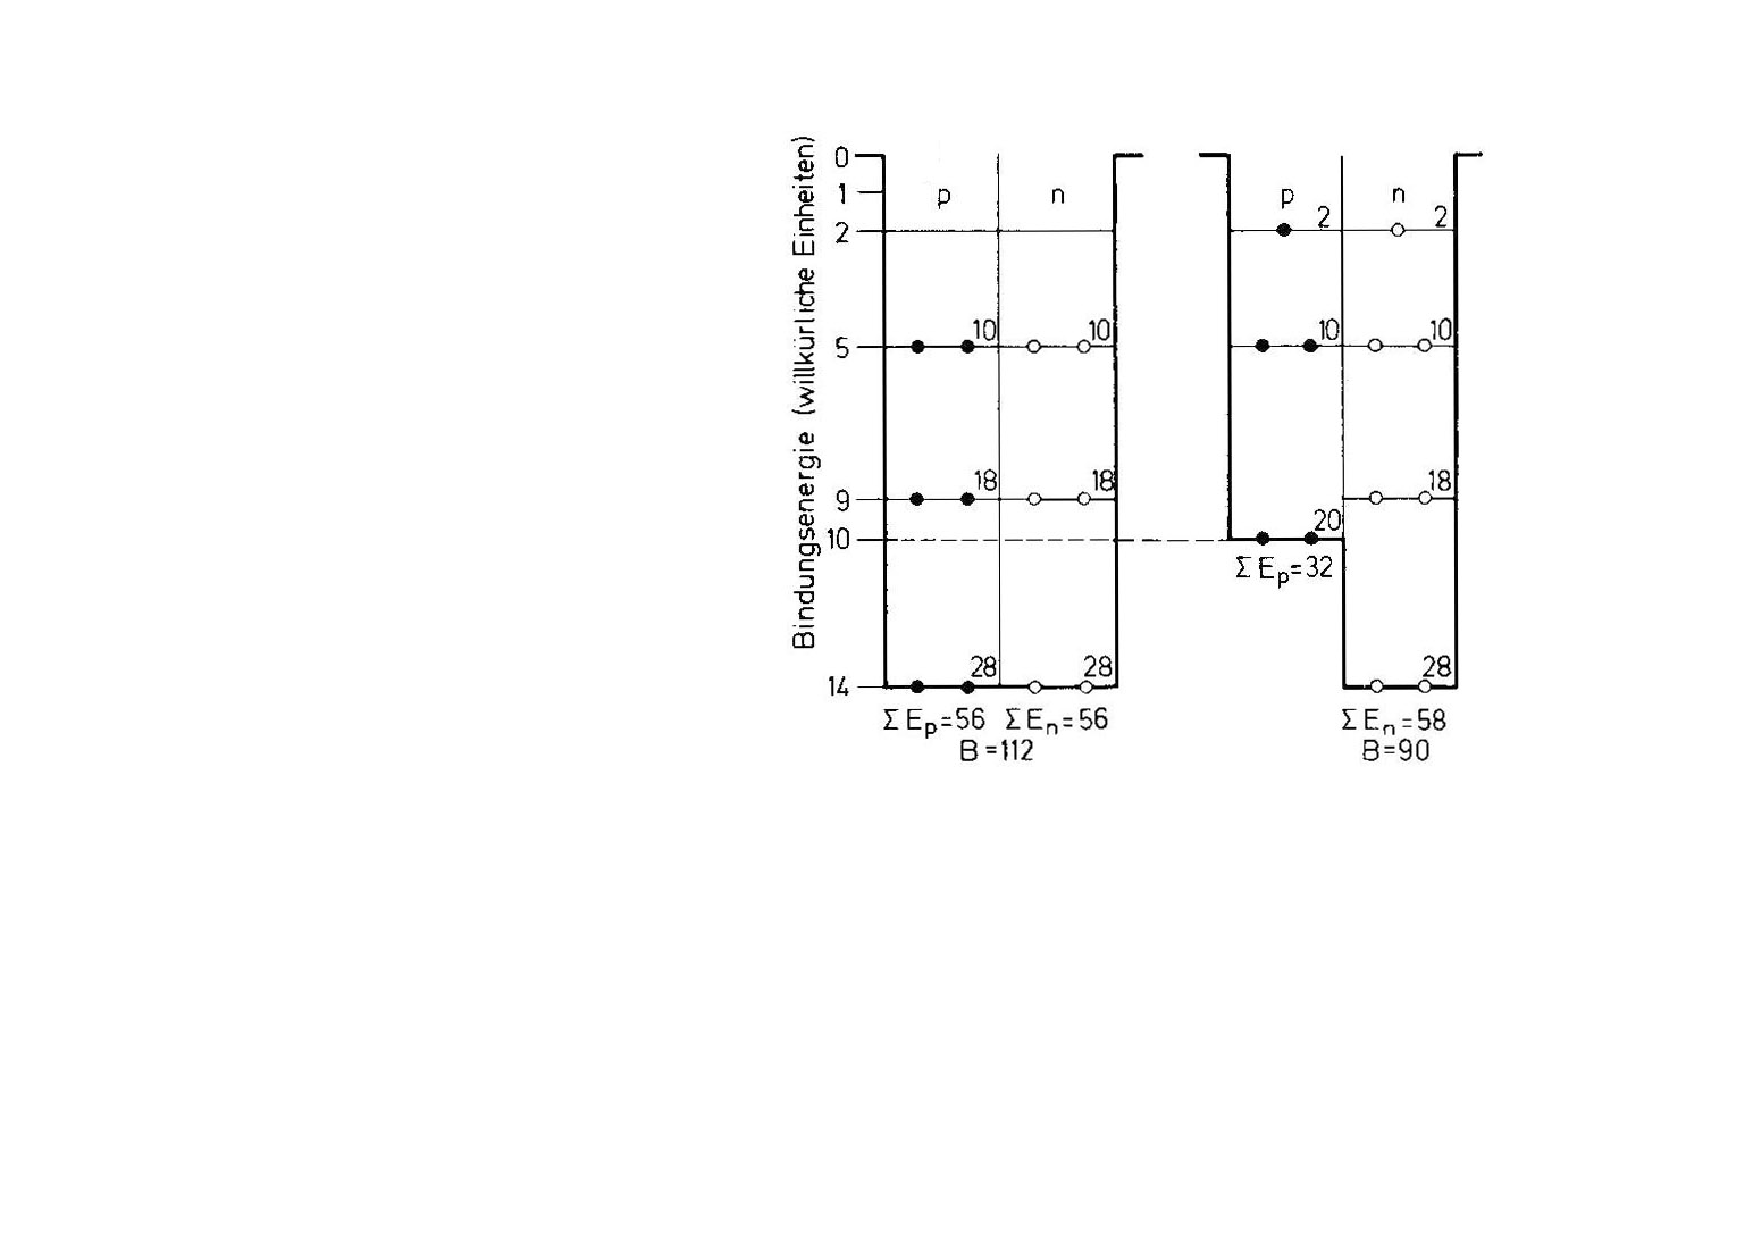
\includegraphics[width=0.8\textwidth]{fig/2-BindungsEnergieMitCoulombPotOhneCoulombPot.pdf}
% 	\caption{Vergleich der Bindungsenergie im symmetrischen (links) und
% 	unsymmetrischen Fermipotential (rechts)}
% \end{figure}

\item Man kann die Schalenstruktur der Kerne anfänglich so erklären, dass man
zum Einfügen eines Fermions in ein ``halb'' gefülltes Niveau kaum Energie
benötigt. Für leichte Kerne erhalten wir jedoch auch durch diese Annahme noch
kein hinreichendes Modell.
\item
Unser Modell ist in keinster Weise vollständig. Man könnte beispielsweise 
anstatt einem Potential mit scharfer Kante eines mit kontinuierlichem Verlauf
annehmen (sog. Wood-Saxon-Potential siehe Abb. \ref{fig:radlad}) und so zu
verbesserten Ergebnissen kommen. Wir werden jedoch sehen, dass das bisher entwickelte Modell für unsere Vorhaben $A>40$ hinreichend
genaue Aussagen macht.\maphere
\end{enumerate}
\end{bemn}

\subsubsection{Tröpfchenmodell}

Das \emph{Tröpfchenmodell} ist ein effektives Modell das auf einer
inkompressiblen Flüssigkeit, die durch kurzreichweitige Wechselwirkung
zusammengehalten wird, basiert. Es kann keine Aussage über die Peaks der
Bindungsenergie pro Nukelon im Bereich weniger Nukleonen machen, dafür
beschreibt es die Gesamtverteilung sehr genau.

Wir werden nun 5 Energien analysieren, die jeweils einen Beitrag zu
Bindungsenergie pro Nukelon leisten, d.h. es gilt
\begin{align*}
E_B = B_1 + B_2 + B_3 + B_4 + B_5.
\end{align*}


\sfigure[!htpb][1]%
	{2-EnergieTermeBWFormel.pdf}
	{\BethgeWalter, S. 49}
	{Bindungsenergie pro Nukleon als Funktion der Massenzahl.}
% 	
% \begin{figure}[!htbp]
% 	\centering
% 	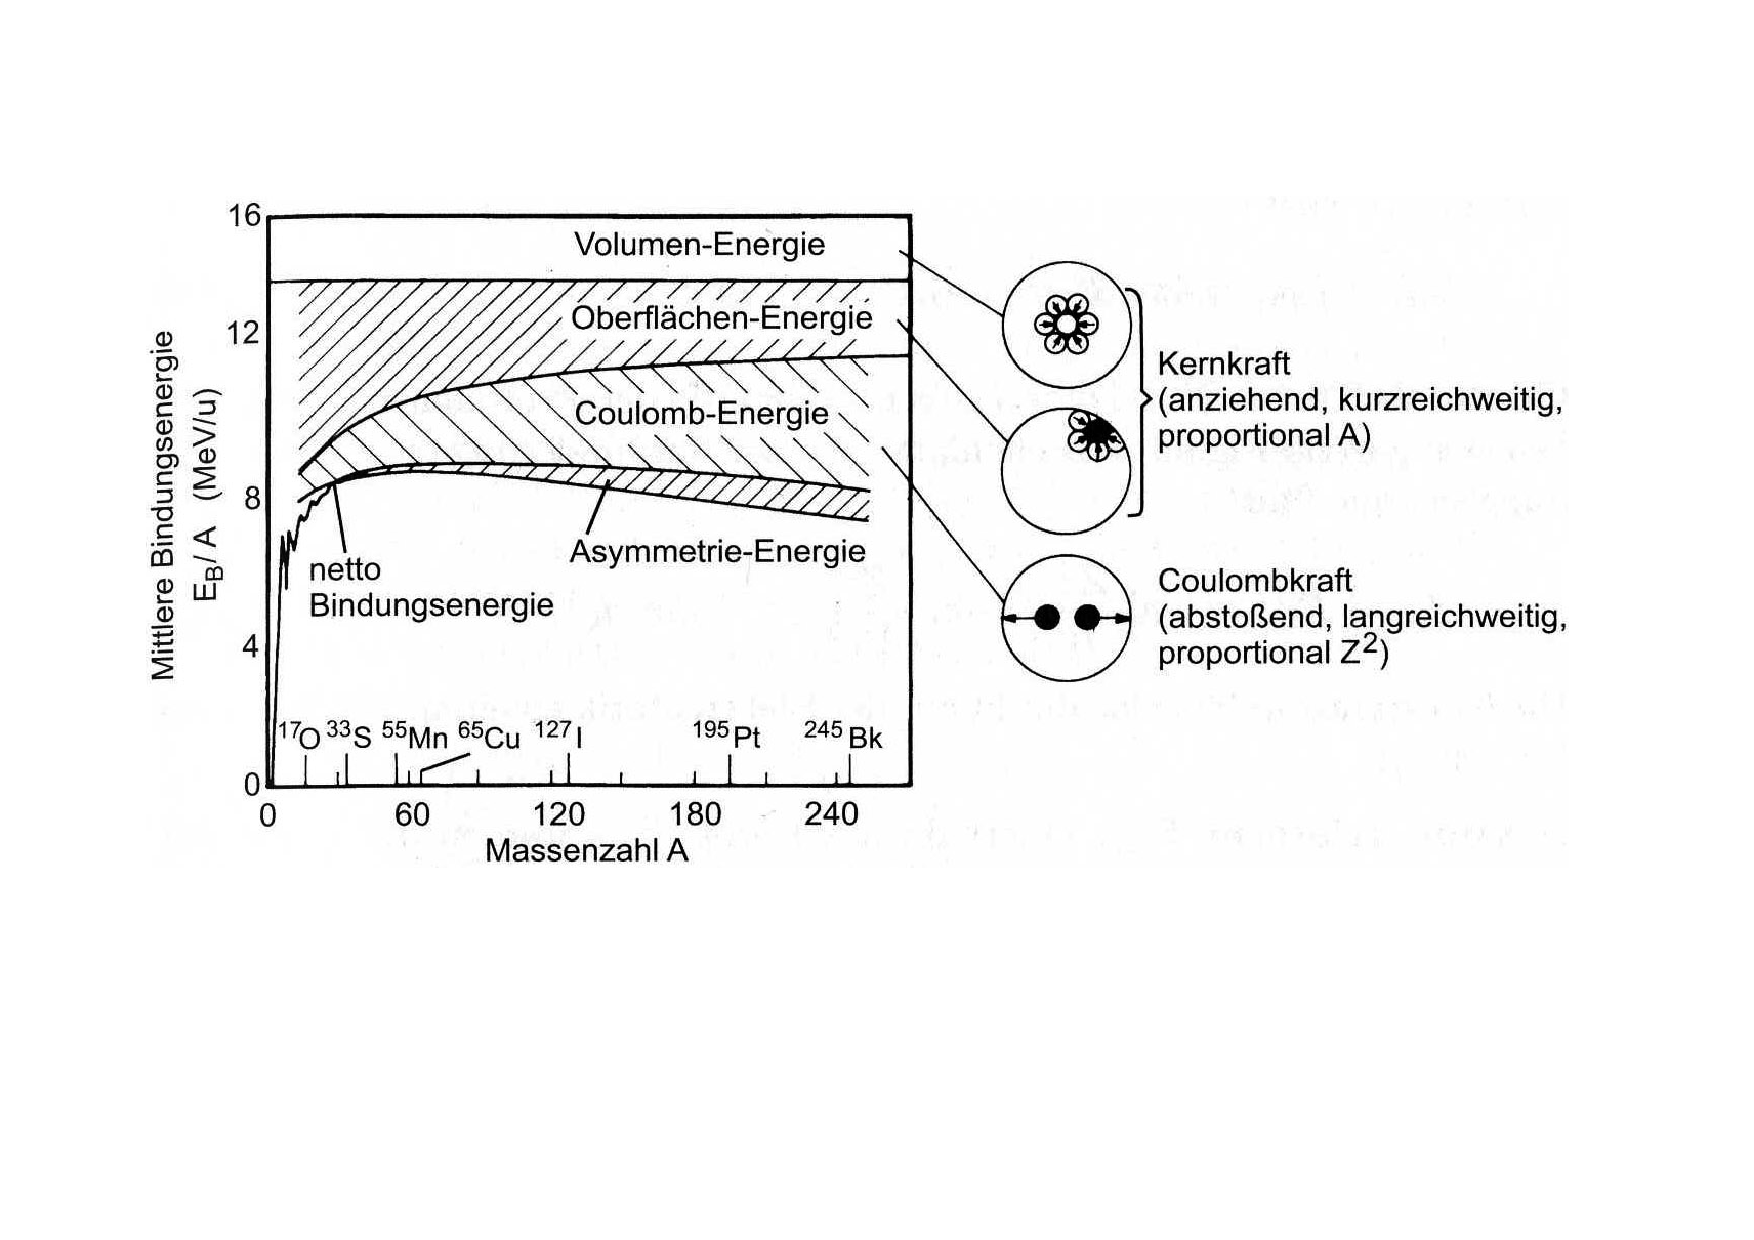
\includegraphics[width=\textwidth]{fig/2-EnergieTermeBWFormel}
% \end{figure}

\begin{enumerate}[label=\arabic{*}.)]
  \item Volumenenergie (Kondensationsenergie)

Wir haben bereits gesehen, dass das Volumen linear in der Nukleonenzahl $A$
ist, d.h.
\begin{align*}
B_1 = a_V A.%,\quad a_V = \frac{B}{A} = \const.
\end{align*}
\item Oberflächenenergie (Oberflächenspannung)

Die Oberfläche $S = 4\pi r_0^2\left(A^{1/3}\right)^2$ nimmt nicht linear mit der
Nukleonenzahl zu,
\begin{align*}
B_2 = -a_S A^{2/3},
\end{align*}
d.h. die Bindungsenergie wird \textit{größer}, wenn sich die Oberfläche
verkleinert.
\item Coulombenergie.

Die Coulombenergie einer homogen geladenen Kugel ist gegeben durch,
\begin{align*}
E = \frac{3}{5}\frac{q^2}{R},
\end{align*}
wobei $R = r_0 A^{1/3}$. Hier leisten nur die postiv geladenen Fermionen einen
Beitrag,
\begin{align*}
B_3 = -a_C \frac{Z^2}{A^{1/3}} = a_C Z^2 A^{-1/3}.
\end{align*}
\item Asymetrieenergie

Die Asymetrieenergie hat ihren Ursprung in der Coulomb-Wechselwirkung, denn
diese führt zum Neutronenüberschuss. Dadurch ändert sich die Zustandsdichte,
was im Fermimodell einer Änderung der Bindungsenergie pro Nukelon hervorruft.

Die Energie im Fermigas mit $n$ Fermionen lässt sich wie folgt abschätzen,
\begin{align*}
E_\tot = \int\limits_0^{E_F} 2E\frac{\dn}{\dE}\dE
\sim V\int\limits_{0}^{E_F} E^{\frac{3}{2}}\dE \sim VE^{\frac{5}{2}}
\sim V\left(\left(\frac{n}{V}\right)^{\frac{2}{3}} \right)^{\frac{5}{2}}
= A^{-\frac{2}{3}}n^{\frac{5}{3}}.
\end{align*}

Ein Atom enthält zwei Arten von Fermionen ($p^+,n^0$), es gilt somit
\begin{align*}
E_\tot = CA^{-\frac{2}{3}}\left(Z^{\frac{5}{3}} + N^{\frac{5}{3}}\right).
\end{align*}
Für einen symmetrischen Kern $N=Z$ erhalten wir so,
\begin{align*}
E_\tot = 2CA^{-\frac{2}{3}}\left(\frac{A}{2}\right)^{\frac{5}{3}} =
\frac{C}{2^{\frac{2}{3}}}A.
\end{align*}
Wie viel Energie kostet von dieser Energie aus ein Neutronenüberschuss $T_Z =
\frac{1}{2}(Z-N)$?
\begin{align*}
\Delta E = CA^{-\frac{2}{3}}\left(Z^{\frac{5}{3}} + N^{\frac{5}{3}} -
2\left(\frac{A}{2}\right)^{\frac{5}{3}}\right)
\end{align*}
Da die Gesamtenergie nicht linear in $n$ ist, ist die Energiedifferenz nicht
Null. Wir wollen $\Delta E$ für keines $T_Z$ entwickeln,
\begin{align*}
\Delta E &= CA^{-\frac{2}{3}}\left(\left(\frac{A}{2} + T_Z\right)^{\frac{5}{3}}
+ \left(\frac{A}{2} - T_Z\right)^{\frac{5}{3}} -
2\left(\frac{A}{2}\right)^{\frac{5}{3}}\right)\\ &
= 2^{-\frac{5}{3}}CA^{-\frac{2}{3}}A^{\frac{5}{3}}\left(
\left(1+\frac{2T_Z}{A}\right)^{\frac{5}{3}}
+\left(1-\frac{2T_Z}{A}\right)^{\frac{5}{3}}
-2 \right).
\end{align*}
Verwende $(1\pm x)^{p} = 1\pm px + \frac{p(p-1)}{2}x^2 + \ldots$,
\begin{align*}
&\Delta E = 2^{-\frac{5}{3}}CA^{-\frac{2}{3}}A^{\frac{5}{3}}\left(
2  + 2\frac{4}{A^2}\frac{10}{9}T_Z^2 - 2\right) = 2^{-\frac{2}{3}}
\frac{80}{9}\frac{T_Z^2}{A},\\ \Rightarrow & B_4 = -a_A \frac{T_Z^2}{A} =
-a_A\frac{\left(Z-\frac{A}{2}\right)^2}{A}
\end{align*}
\item Paarbildungsenergie.

Die Paarbildungsenergie muss empirisch eingeführt werden, um der Beobachtung
gerecht zu werden. Betrachten wir die Neutronen und Protonen Energiniveaus, so
können die jeweils gerade (g) oder ungerade (u) besetzt sein. Die
Beobachtung zeigt, dass (gg) Kerne besonders stabil und (uu) Kerne weniger
gebunden sind. Es ist energetisch günstig ein Nukelon in ein bereits halb
besetztes Energieniveau einzufügen.

Wir wollen dies durch folgenden Term berücksichtigen.
\begin{align*}
B_5 = \begin{cases}      
+\delta, & \text{für gg},\\
0, & \text{für ug/gu},\\
-\delta, & \text{für uu}.
\end{cases}
\end{align*} 
\end{enumerate}
Alle fünf Terme zusammen führen zur \emph{Bethe-Weizsäcker-Formel} mit der sich
die Bindungsenergie pro Nukelon vorhersagen lässt,
\begin{align*}
&E_B = B_1 + B_2 + B_3 + B_4 + B_5
= a_V A -a_S A^{2/3}-a_C
\frac{Z^2}{A^{1/3}}-a_A\frac{\left(Z-\frac{A}{2}\right)^2}{A}\pm \delta,\\
& m(Z,N) = N\cdot m_{n^0} + Z m_{p^+} - \frac{E_B}{c^2}. 
\end{align*}
Für schwere Kerne erreicht die Formel eine Präzission von einem Prozent. Wir
werden sehen, dass wir sogar Kernzerfälle mithilfe dieser Formel vorhersagen
können.

\noindent\textit{Interpretation der Bethe-Weizsäcker-Formel.}
%\begin{bemn}[]
\begin{enumerate}[label=\arabic{*})]
  \item Das Maximum der Bindungsenergie pro Nukleon $\frac{B}{A}$ kommt durch
  die Abnahme der Oberflächenenergie und der Zunahme der Coulombenergie
  zustande.
  \item Schaleneffekte für kleine $A$ werden nicht berücksichtig. Für $A>40$
  beschreibt die Formel $\frac{B}{A}$ jedoch auf 1 Prozent genau.
  \item Mithilfe der Formel lassen sich Aussagen über die Stabilität der Kerne machen.
  
  Betrachten wir Isobare, d.h. $A=\const$, in der Nähe von $N(Z,A)\sim Z^2$.
  Für $A$ ungerade erhalten wir folgendes Zerfallsschema.
\begin{figure}[H]
  \centering
\begin{pspicture}(1,-1.5)(7,1.5)
\psaxes[labels=none,ticks=none]{->}%
(4,-0.75)(1.6,-0.95)(6.4,1.25)[\color{gdarkgray}$Z$,-90][\color{gdarkgray}$m$,0]
\psbezier(1.86,0.7981994)(2.26,-1.2798958)(5.776432,-1.2598958)(6.16,0.90010417)
\pscircle[fillstyle=solid,fillcolor=white](2.78,-0.29989582){0.12}
\pscircle[fillstyle=solid,fillcolor=white](2.06,0.54010415){0.12}
\pscircle[fillstyle=solid,fillcolor=gdarkgray](4.0,-0.6198958){0.12}
\pscircle[fillstyle=solid,fillcolor=white](5.18,-0.29989582){0.12}
\pscircle[fillstyle=solid,fillcolor=white](5.9,0.54010415){0.12}
\psbezier[linecolor=darkblue,linestyle=dotted,dotsep=0.06cm]{->}(2.18,0.36010417)(2.3,0.10010417)(2.4,0.020104166)(2.62,-0.15989584)
\psbezier[linecolor=darkblue,linestyle=dotted,dotsep=0.06cm]{->}(2.98,-0.39989585)(3.24,-0.57989585)(3.48,-0.59989583)(3.84,-0.6198958)
\psbezier[linecolor=yellow,linestyle=dotted,dotsep=0.06cm]{->}(5.02,-0.39989585)(4.76,-0.57989585)(4.52,-0.59989583)(4.16,-0.6198958)
\psbezier[linecolor=yellow,linestyle=dotted,dotsep=0.06cm]{->}(5.82,0.36010417)(5.7,0.10010417)(5.6,0.020104166)(5.38,-0.15989584)

\rput(3.7626562,-1.0098958){\color{gdarkgray}$Z_0$}
\rput(5.5242186,0.35010415){\color{gdarkgray}$\beta^+$}
\rput(4.624219,-0.26989582){\color{gdarkgray}$\beta^+$}
\rput(3.3042188,-0.26989582){\color{gdarkgray}$\beta^-$}
\rput(2.5242188,0.31010416){\color{gdarkgray}$\beta^-$}
\end{pspicture} 
  \caption{Zerfallsschema für Isobare mit $A$ ungerade. Stabiler Kern ist
  ausgefüllt.}
\end{figure}
  Wir können somit konkret ausrechnen, welche Energie die Elektronen beim
  $\beta$-Zerfall haben.
  
 \begin{figure}[!ht]
  \centering
\begin{pspicture}(0.5,-1.65)(7.5,2)
\psaxes[labels=none,ticks=none]{->}%
(4,-0.95)(1,-1)(7,1.7)%
[\color{gdarkgray}$Z$,-90][\color{gdarkgray}$m$,0]

\psbezier(1.14,0.590077)(1.6832558,-1.5070833)(6.459061,-1.4868999)(6.98,0.6929167)
\pscircle[fillstyle=solid,fillcolor=white](3.0,0.91291666){0.12}
\pscircle[fillstyle=solid,fillcolor=gdarkgray](1.44,0.19291666){0.12}
\pscircle[fillstyle=solid,fillcolor=gdarkgray](4.0,-0.82708335){0.12}
\pscircle[fillstyle=solid,fillcolor=white](5.16,0.91291666){0.12}
\pscircle[fillstyle=solid,fillcolor=gdarkgray](6.62,0.19291666){0.12}

\psbezier(2.02,1.5910119)(3.12,0.19291666)(5.06,0.17291667)(6.32,1.6929166)
\psline[linecolor=yellow,linestyle=dotted,dotsep=0.06cm]{->}(5.4,0.7729167)(6.46,0.25291666)
\psline[linecolor=darkblue,linestyle=dotted,dotsep=0.06cm]{->}(5.0,0.61291665)(4.2,-0.64708334)
\psline[linecolor=yellow,linestyle=dotted,dotsep=0.06cm]{->}(2.66,0.7529167)(1.6,0.23291667)
\psline[linecolor=darkblue,linestyle=dotted,dotsep=0.06cm]{->}(3.06,0.59291667)(3.86,-0.6670833)

\rput(3.7626562,-1.2170833){\color{gdarkgray}$Z_0$}
\rput(6.981406,0.1){\color{gdarkgray}\small$gg$}
\rput(1,0.1){\color{gdarkgray}\small$gg$}
\rput(2.8595312,1.28){\color{gdarkgray}\small$uu$}
\rput(5.4195313,1.28){\color{gdarkgray}\small$uu$}
\psline[linestyle=dotted,dotsep=0.06cm]{->}(1.6,0.09291667)(3.76,-0.8070833)
\psline(2.68,-0.18708333)(2.44,-0.40708333)
\psline[linestyle=dotted,dotsep=0.06cm]{->}(6.42,0.11291666)(4.26,-0.7870833)
\psline(5.34,-0.16708334)(5.58,-0.38708332)

\rput(1.9242188,0.7029167){\color{gdarkgray}$\beta$}
\rput(3.5042188,0.24291667){\color{gdarkgray}$\beta$}
\rput(4.5642185,0.24291667){\color{gdarkgray}$\beta$}
\rput(6.144219,0.7029167){\color{gdarkgray}$\beta$}
\end{pspicture} 
  \caption{Zerfallsschema für Isobare mit $A$ gerade. Stabile Kerne sind
  ausgefüllt.}
\end{figure}

 Für $A$ gerade ist $\Delta p^+ = 2k$, um von einem gg zu einem anderen gg zu
 kommen. Es gibt jedoch keinen $\beta$-Zerfall bei dem sich die
 Protonenzahl um ein Vielfaches von $2$ ändert. Daher gibt es viele stabile
 $gg$ Isotope.
\item Man kann mit der Formel auch die stabilsten Kerne vorhersagen, indem man
 die Bindungsenergie maximiert.
\begin{align*}
\frac{\partial m(Z,A=Z+N)}{\partial Z}\bigg|_{N=\const} = 0.
\end{align*}
% 
% \begin{figure}[!htbp]
% 	\centering
% 	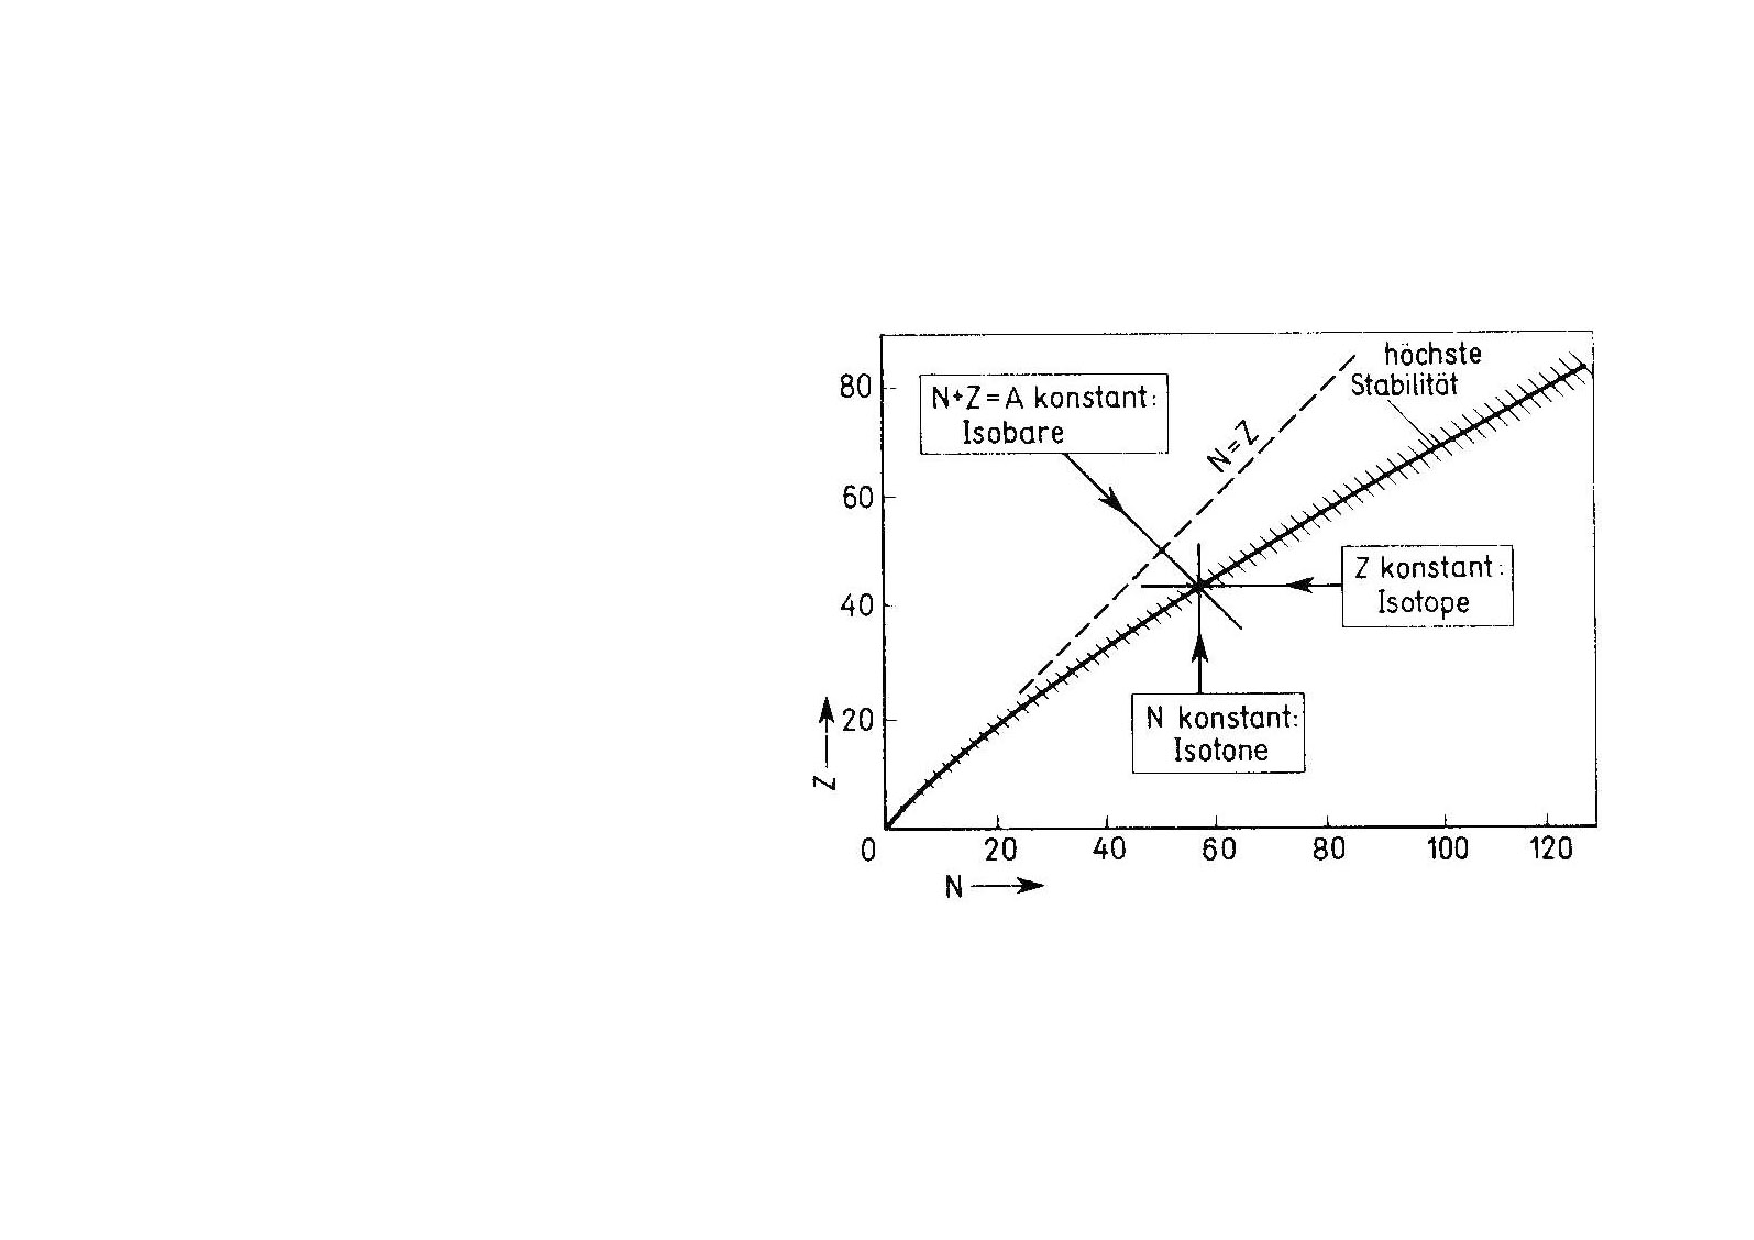
\includegraphics[width=0.9\textwidth]{fig/2-LageStabileKerneNZEbene.pdf}
% \end{figure}


\sfigure[!htpb][0.5]%
	{2-LageStabileKerneNZEbene.pdf}
	{\KuckukKern, S. 53}
	{Lage der stabilen Kerne in der $N$-$Z$-Ebene.}

\item
Beim $\alpha$-Zerfall wird ein $He$-Kern $(2p^+,2n^0)$ emittiert,
\begin{align*}
{}_Z^A  X \overset{\alpha}{\longrightarrow} {}_{Z-2}^{A-4} X + \alpha^{2+}.
\end{align*}
Die Energiebilanz des $\alpha$-Zerfalls ist,
\begin{align*}
E_\alpha = \left[m(Z,A) - m(Z-2,A-4) - m_\alpha\right]c^2.
\end{align*}
Für $E_\alpha > 0$ ist der Zerfall möglich, für wachsendes $E_\alpha$ wird der
Prozess schneller. Man kann dies mit dem Modell von Gamov
beschreiben.
\begin{figure}[!ht]
  \centering
% Generated with LaTeXDraw 2.0.3
% Mon Jul 13 20:26:46 CEST 2009
% \usepackage[usenames,dvipsnames]{pstricks}
% \usepackage{epsfig}
% \usepackage{pst-grad} % For gradients
% \usepackage{pst-plot} % For axes
\scalebox{1} % Change this value to rescale the drawing.
{
\begin{pspicture}(0,-1.78)(4.4,1.78)
\psbezier(1.3941112,0.435)(1.3941112,1.115)(1.36,1.56)(1.5,1.56)(1.64,1.56)(1.82,1.32)(2.08,1.04)(2.34,0.76)(2.72,0.4)(3.9,0.4)
\psline(1.3941112,0.495)(1.374111,-1.405)(0.014111111,-1.405)(0.0,1.72)
\pscircle(0.6341111,1.255){0.22}
\psline[linestyle=dotted,dotsep=0.06cm]{->}(1.0341111,1.22)(3.82,1.22)
\psline{->}(1.38,0.4)(4.28,0.4)
\psline(1.92,1.2)(1.92,0.4)
\psdots[dotsize=0.12](0.12,-1.4)
\psdots[dotsize=0.12](0.52,-1.4)
\psdots[dotsize=0.12](0.12,-1.0)
\psdots[dotsize=0.12](0.52,-1.0)
\psdots[linecolor=darkblue,dotsize=0.12](0.12,0.6)
\psdots[linecolor=darkblue,dotsize=0.12](0.52,0.6)
\psdots[dotsize=0.12](0.12,-0.6)
\psdots[dotsize=0.12](0.52,-0.6)
\psdots[dotsize=0.12](0.12,-0.2)
\psdots[dotsize=0.12](0.52,-0.2)
\psdots[dotsize=0.12](0.12,0.2)
\psdots[dotsize=0.12](0.52,0.2)
\psdots[linecolor=yellow,dotsize=0.12](0.88,0.6)
\psdots[linecolor=yellow,dotsize=0.12](1.28,0.6)
\psdots[dotsize=0.12](0.88,0.36)
\psdots[dotsize=0.12](1.28,0.36)
\psdots[dotsize=0.12](0.88,0.1)
\psdots[dotsize=0.12](1.28,0.1)
\psdots[dotsize=0.12](0.88,-0.2)
\psdots[dotsize=0.12](1.28,-0.2)
\psdots[dotsize=0.12](0.88,-0.54)
\psdots[dotsize=0.12](1.28,-0.54)
\psdots[dotsize=0.12](0.88,-0.88)
\psdots[dotsize=0.12](1.28,-0.88)

\psline{->}(0.62,0.7)(0.62,1.02)
\psline{<->}(3.52,1.18)(3.52,0.44)

\rput(1.55,0.225){\color{gdarkgray}$r_1$}
\rput(2.09,0.225){\color{gdarkgray}$r_2$}
\rput(0.31,-1.575){\color{gdarkgray}$n$}
\rput(1.09,-1.555){\color{gdarkgray}$p$}
\rput(0.62,1.665){\color{gdarkgray}$\alpha$}
\rput(3.92,0.765){\color{gdarkgray}$E_\kin$}
\rput(4.3,0.225){\color{gdarkgray}$r$}
\end{pspicture} 
}

  \caption{Gamovs Erklärung des $\alpha$-Zerfalls.}
\end{figure}

Damit der $\alpha$-Zerfall stattfindet, muss das im Kern entstehende
$\alpha$-Teilchen eine große Barriere, hervorgerufen durch die starke
Kernbindung, überwinden. Kann dadurch Energie frei werden, so existiert eine
bestimmte Wahrscheinlichkeit, dass das Teilchen durch die Barriere tunnelt.
Nach dem Tunneln erhält das $\alpha$-Teilchen eine große kinetische Energie
und kann aufgrund der Barriere nicht mehr in den Kern
zurückkehren. Für die Tunnelwahrscheinlichkeit gilt,
\begin{align*}
\text{Wsk} \sim \exp\left\{\text{Freiwerdende Energie}\right\}.
\end{align*}
\item Die Formel erklärt ebenfalls, warum nur $\alpha$- und $\beta$-Zefälle
auftreten und nicht etwa nur $p^+$ oder $n^0$ emittiert werden. Da
das $\alpha$-Teilchen bereits eine sehr hohe Bindungsenergie hat, ist es
in den meisten Fällen die günstigste Zerfallsvariante. In der Formel ist eine
Änderung von $Z$ oder $N$ um 1 stets ungünstiger als der $\alpha$-Zerfall.
\item Auch für die Kernspaltung kann mit der Bethe-Weizsäcker-Formel eine
Energiebilanz aufgestellt werden. Gilt
\begin{align*}
m(Z,A) > 2m\left(\frac{Z}{2},\frac{A}{2}\right),
\end{align*}
so ist die Spaltung energetisch möglich. Jedoch ist auch hier - wie beim
$\alpha$-Zerfall - eine Barriere zu überwinden.

% \begin{figure}[!htbp]
% 	\centering
% 	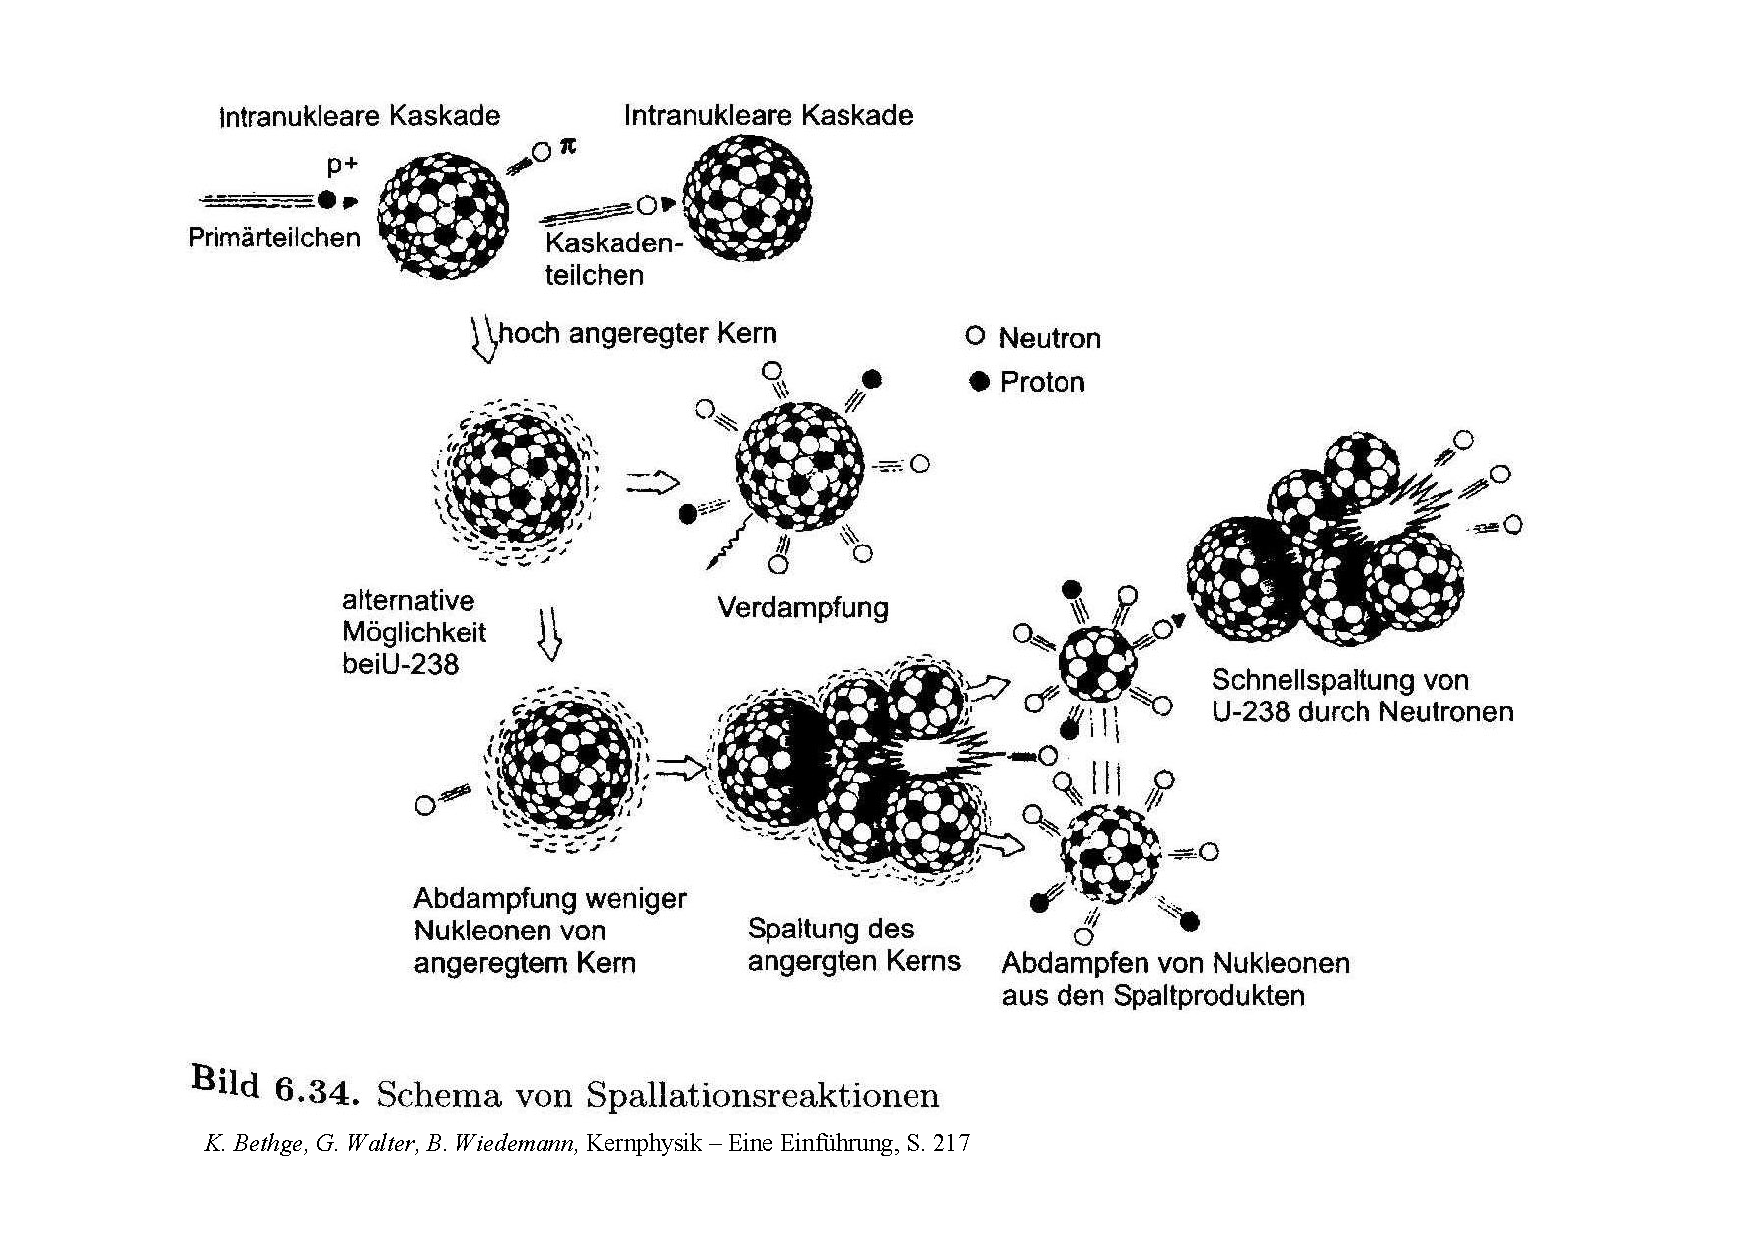
\includegraphics[width=0.9\textwidth]{fig/2-Kernspaltung.pdf}
% \end{figure}

 Man hat von zahlreichen
Nukleonen die Halbwertszeit $\tau_{1/2}$ bestimmt und stellte fest, dass
\begin{align*}
\tau_{1/2} \sim \frac{1}{\lambda},
\end{align*}
wobei $\lambda$ die Tunnelwahrscheinlichkeit des $\alpha$-Teilchens
bezeichnet. Diesen Zusammenhang nennt man die \emph{Geiger-Nuttall-Regel}. Im
Experiment sieht man eine Übereinstimmung über 25 Größenordnungen hinweg.
% 
% \begin{figure}[!htbp]
% 	\centering
% 	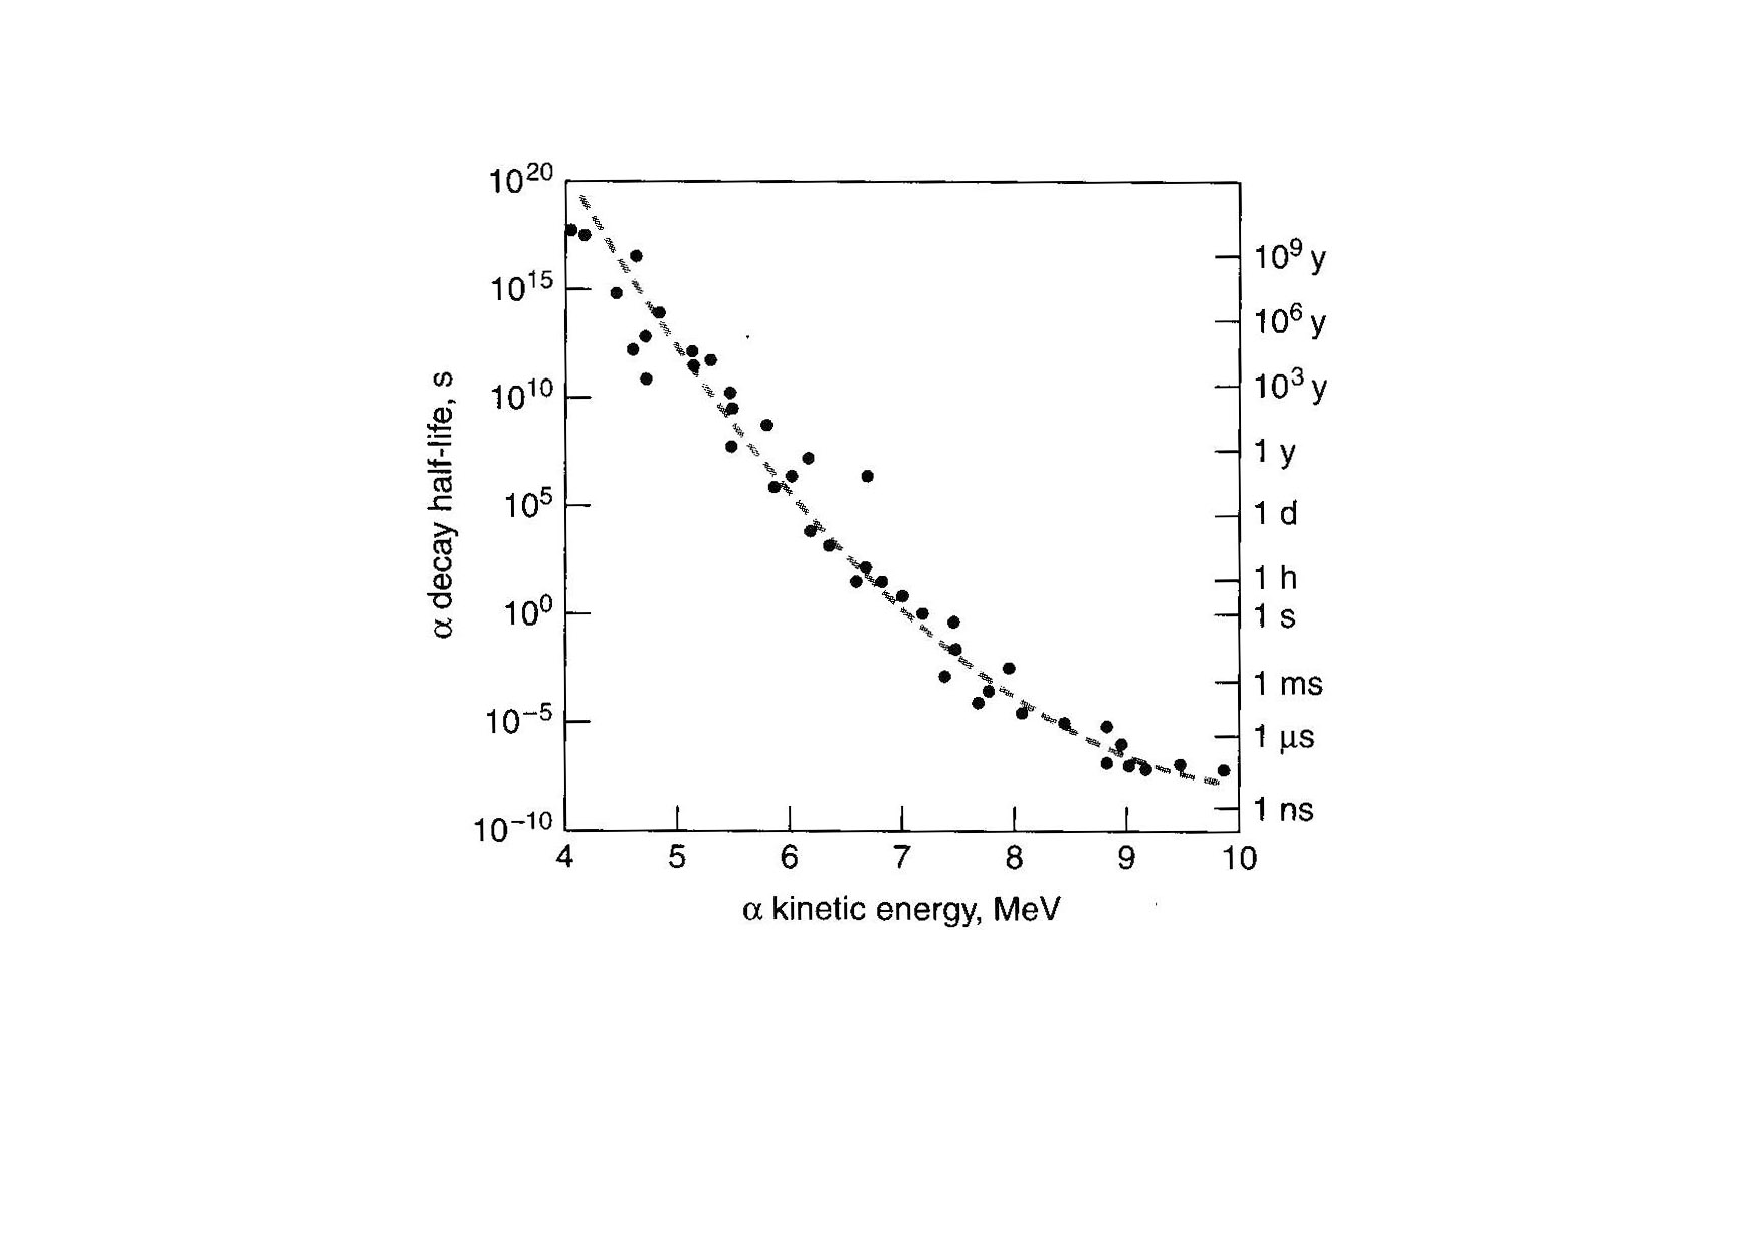
\includegraphics[width=0.9\textwidth]{fig/2-GeigerNuttallRegel.pdf}
% \end{figure}
% 

\sfigure[!htpb][0.7]%
	{2-GeigerNuttallRegel.pdf}
	{\TiplerMPFife, S. 496}
	{Halbwertszeit des $\alpha$-Zefalls
	für natürlich vorkommende Zerfälle halblogarithmisch über der kinetischen
	Energie der $\alpha$ Teilchens aufgetragen. Die gestrichelte Linie stellt die
	Vorhersage der Geiger-Nuttall Regl dar.}


Die Tunnelwahrscheinlichkeit für eine spontane Spaltung ist typischerweise
viel kleiner als die für den $\alpha$-Zerfall. Man kann jedoch durch 
Neutroneneinfang Energie in das System einbringen und dadurch die Spaltung
induzieren.

Der Kernspaltungsprozess zeigt Analogieen zur Verformung von elastischen
Körpern. Die für eine Spaltung zu überwindende Potentialbarriere ist in diesem
Modell vergleichbar mit einem Riss der Oberfläche.

\sfigure%
	{2-SpaltDeformation.pdf}
	{\BethgeWalter, S. 244}
	{Einfache (gestrichelt) und doppelhöckrige Spaltbarriere.}
% 
% \begin{figure}[!htbp]
% 	\centering
% 	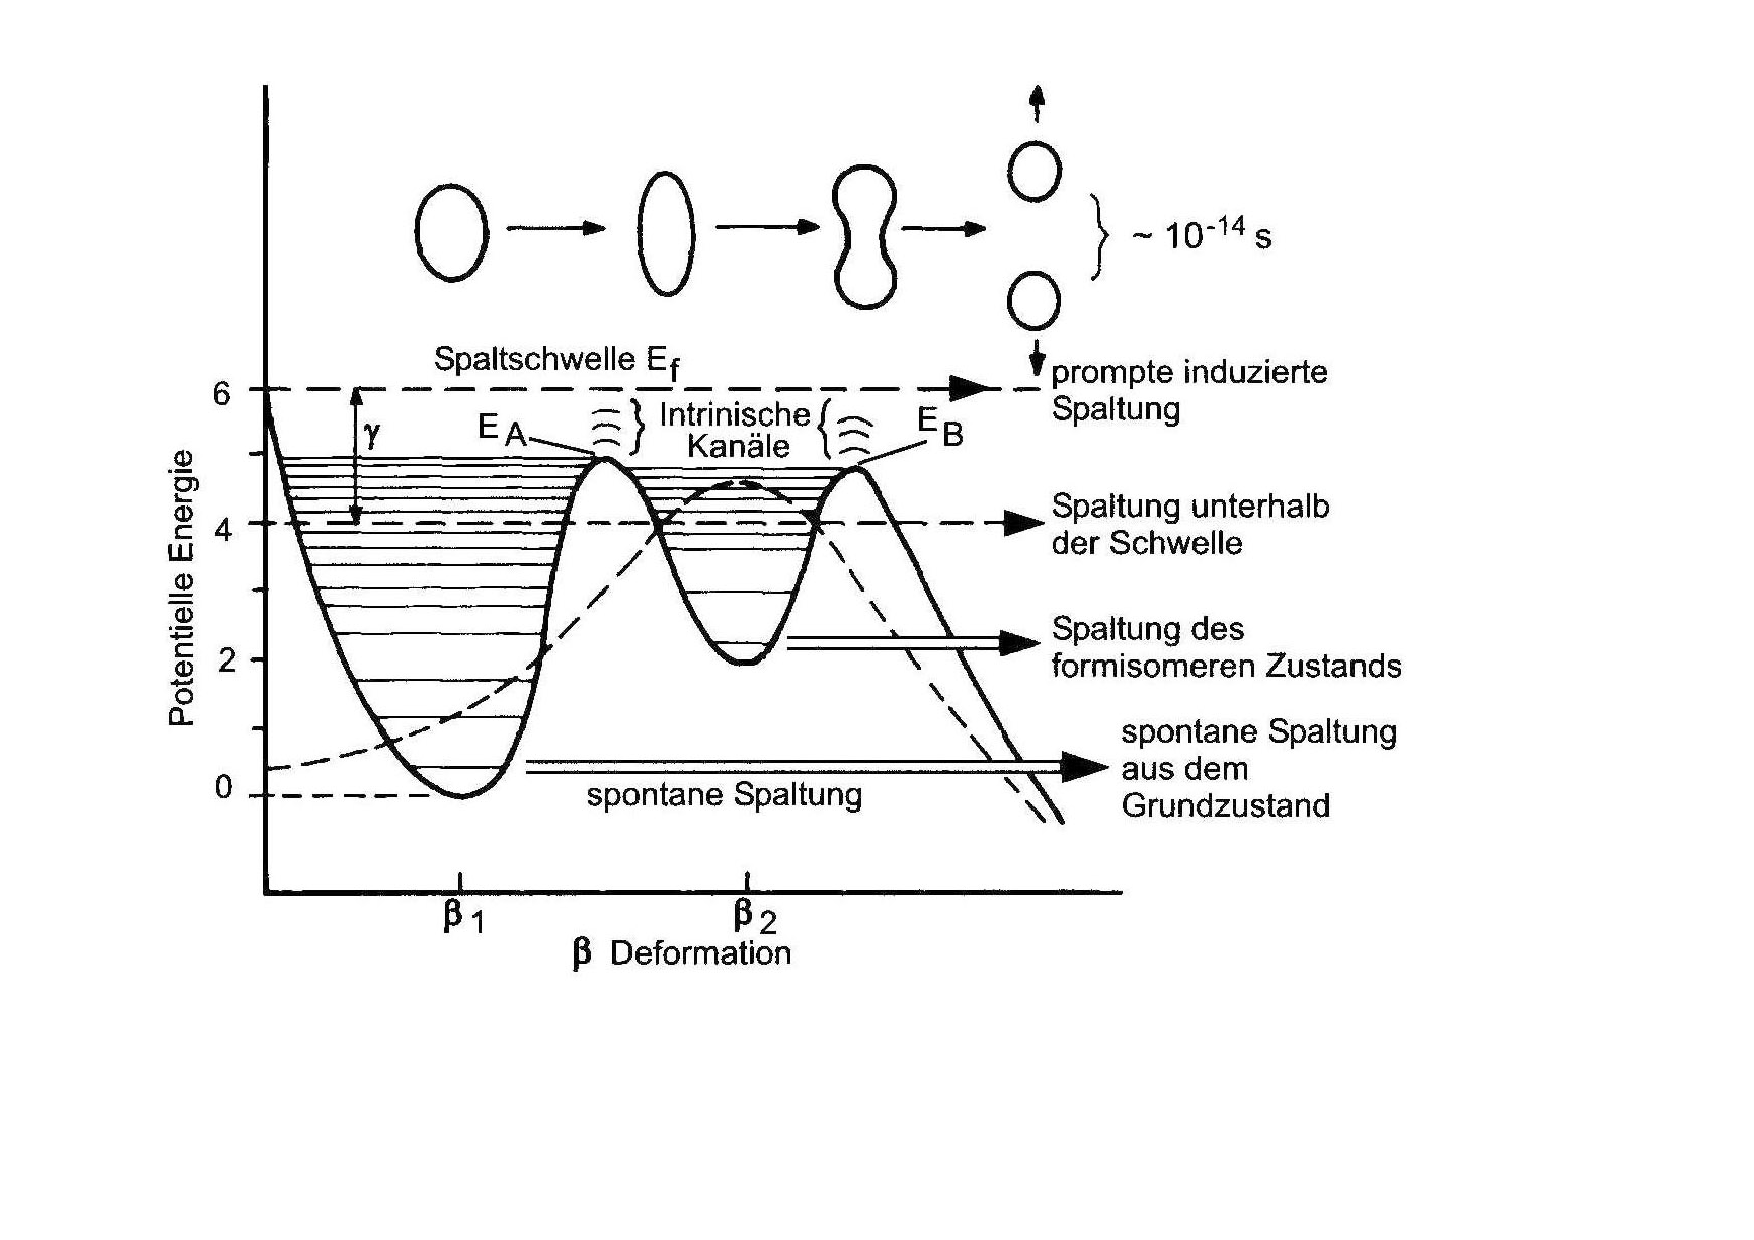
\includegraphics[width=\textwidth]{fig/2-SpaltDeformation.pdf}
% \end{figure}

\begin{bspn}
Bei Uran 235 ist die günstigste Spaltung nicht die Halbierung sondern die
Teilung in einem schweren $\sim 140\mathrm{u}$ und einen leichten $\sim
90\mathrm{u}$ Kern. Auch dies folgt aus der Bethe-Weizsäcker-Formel und ist für
viele weitere Kerne der Fall.\bsphere
\end{bspn}

% 	
% \begin{figure}[H]
% 	\centering
% 	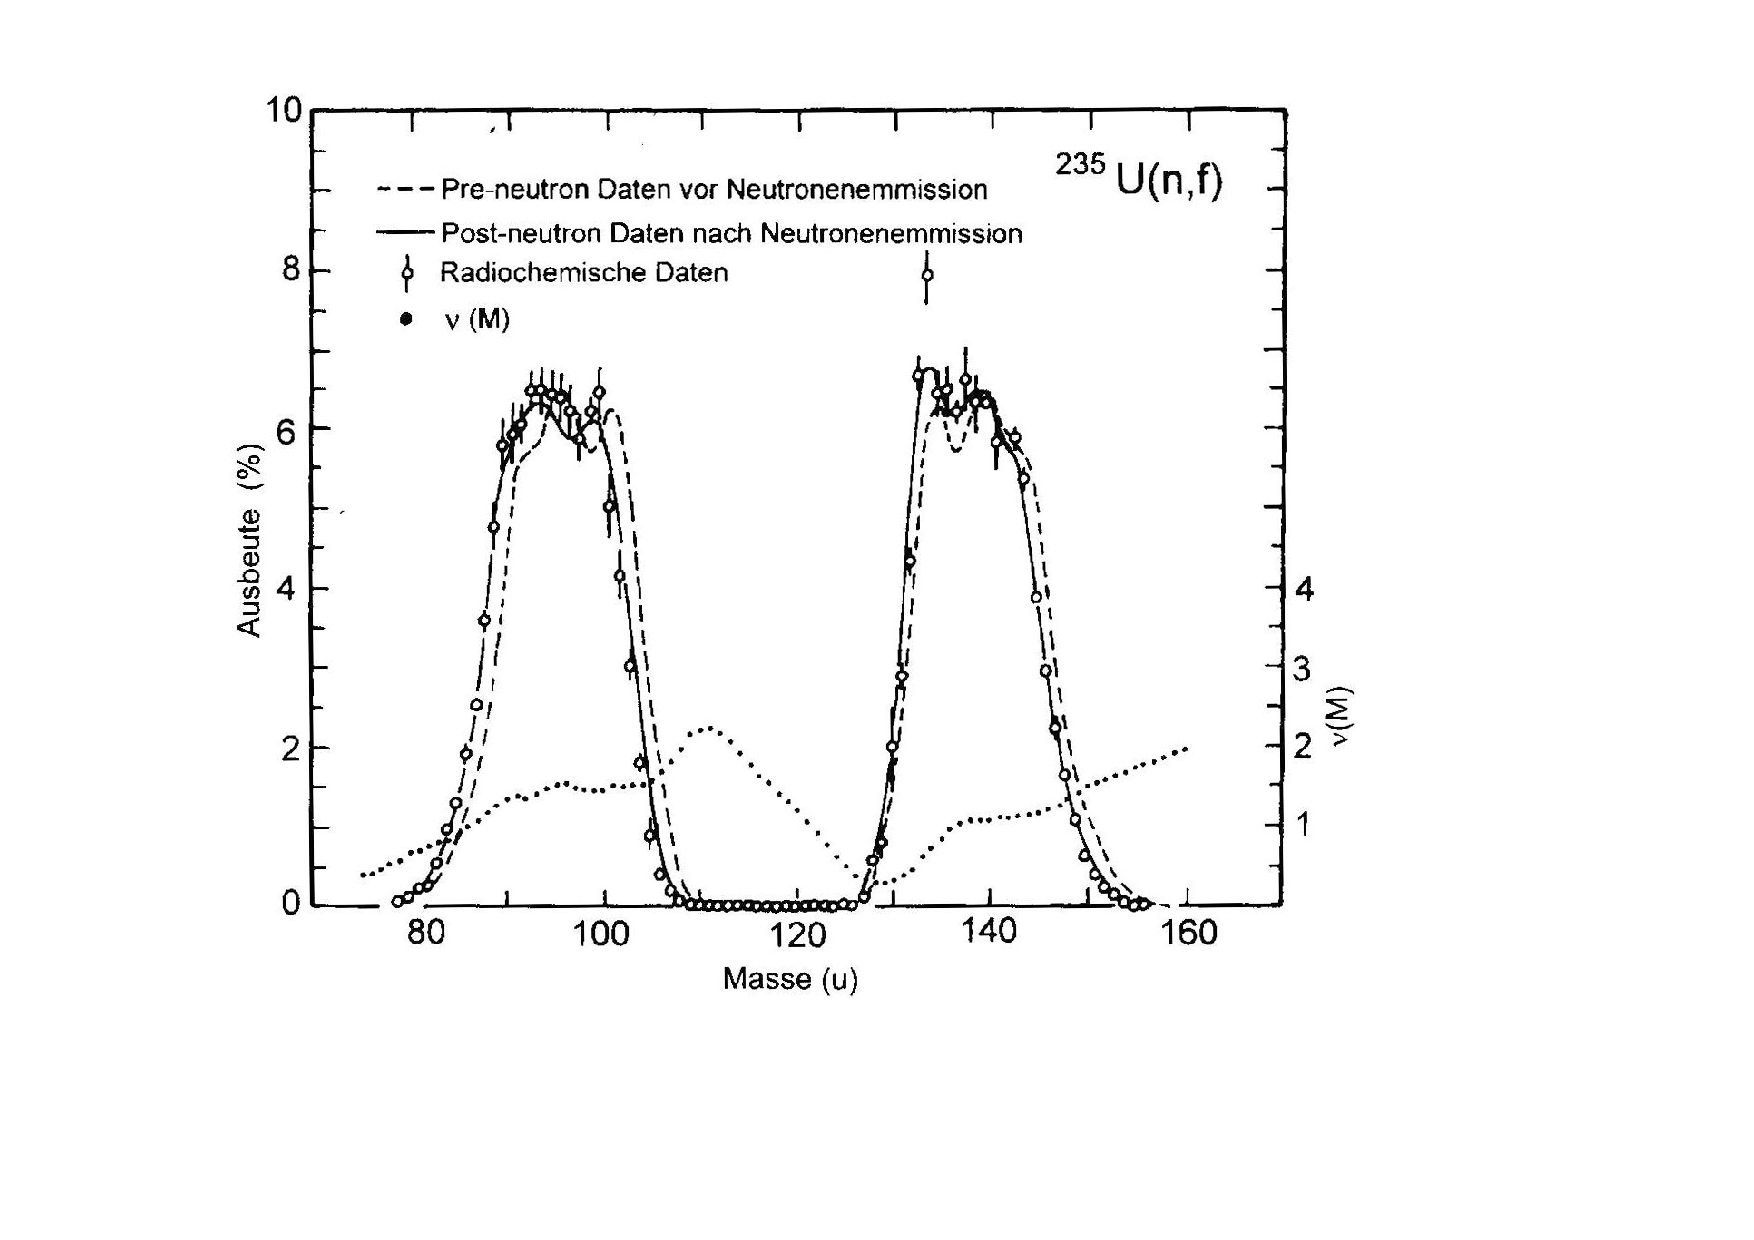
\includegraphics[width=\textwidth]{fig/2-MassenverteilungSpaltfragmenteUran.pdf}
% \end{figure}


\sfigure[H][0.7]%
	{2-MassenverteilungSpaltfragmenteUran.pdf}
	{\BethgeWalter, S. 240}
	{Massenverteilung der Spaltfragmente aus ${}^{235}\mathrm{U}(n,f)$. Die
	gepunktete Linie gibt die mittlere Anzahl der emittierten Neutronen $\nu(M)$
	aus.}
	
% 	\begin{figure}[!htbp]
% 	\centering
% 	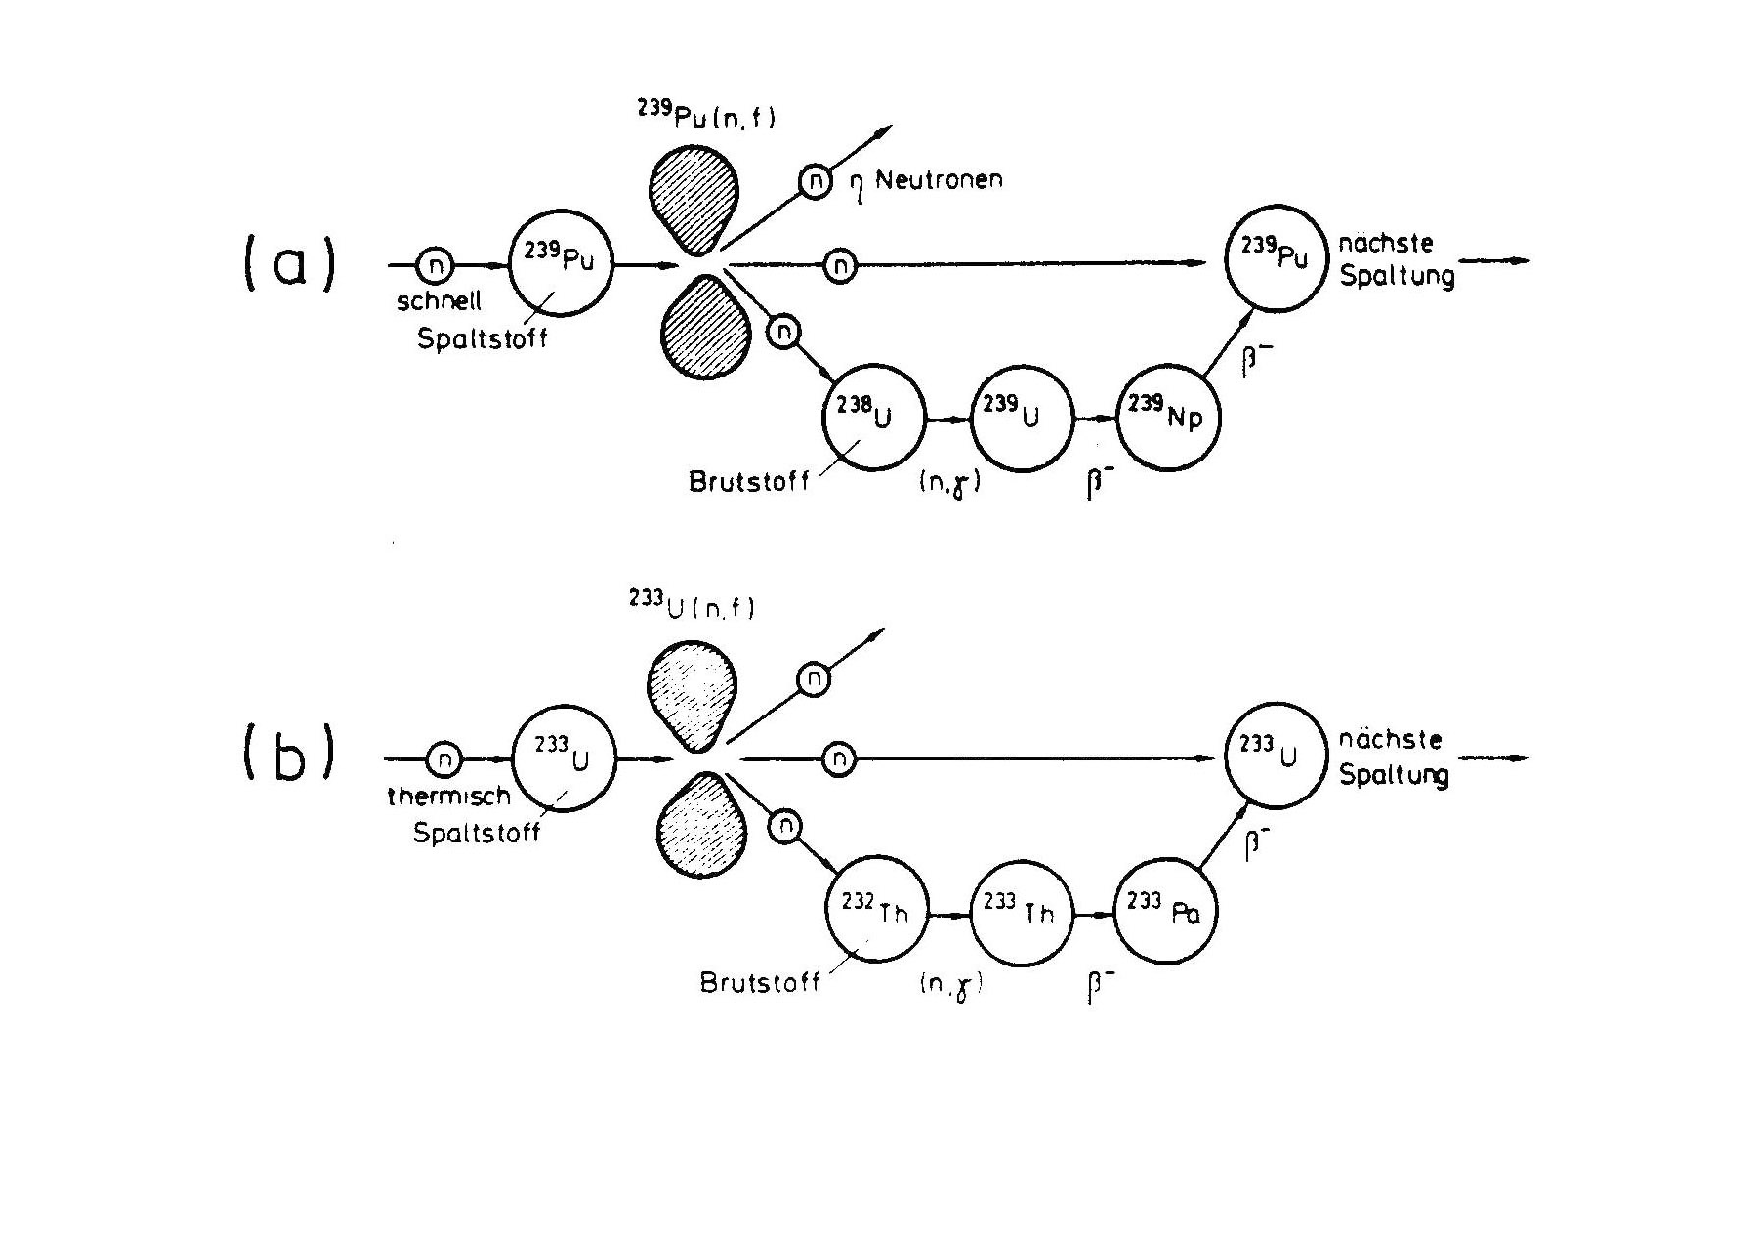
\includegraphics[width=\textwidth]{fig/2-SpaltBrutKetten.pdf}
% \end{figure}

\sfigure[H][0.7]%
	{2-SpaltBrutKetten.pdf}
	{\KuckukKern, Fig. 127}
	{Spalt-Brutketten. a) Schneller Brüter, b) Thorium-Brüter.}


\begin{bspn}
Berücksichtigt man zusätzlich noch die Schalenstruktur der Kerne, so lässt sich im Bereich
von $Z\sim 120$, $N\sim 190$ eine ``Insel der Stabilität'' vorhersagen, d.h. es
könnte dort bisher unentdeckte aber stabile Elemente geben. Es stellt sich jedoch als
äußerst schwierig heraus, diese
``Superschweren Kerne'' zu erzeugen.\bsphere
\end{bspn}


\sfigure[H]%
	{2-StabilitaetsGebirge.pdf}
	{\KuckukKern, Fig. 55}
	{Bindungsenergien der Kerne in Abhängigkeit von $Z$ und $N$. Nur die aus der
	Obefläche herausragenden Kerne sind stabil. Bei $N\approx 190$ befindet sich
	die spekulative Stabilitätsinsel.}

\begin{figure}[H]
	\centering
% 	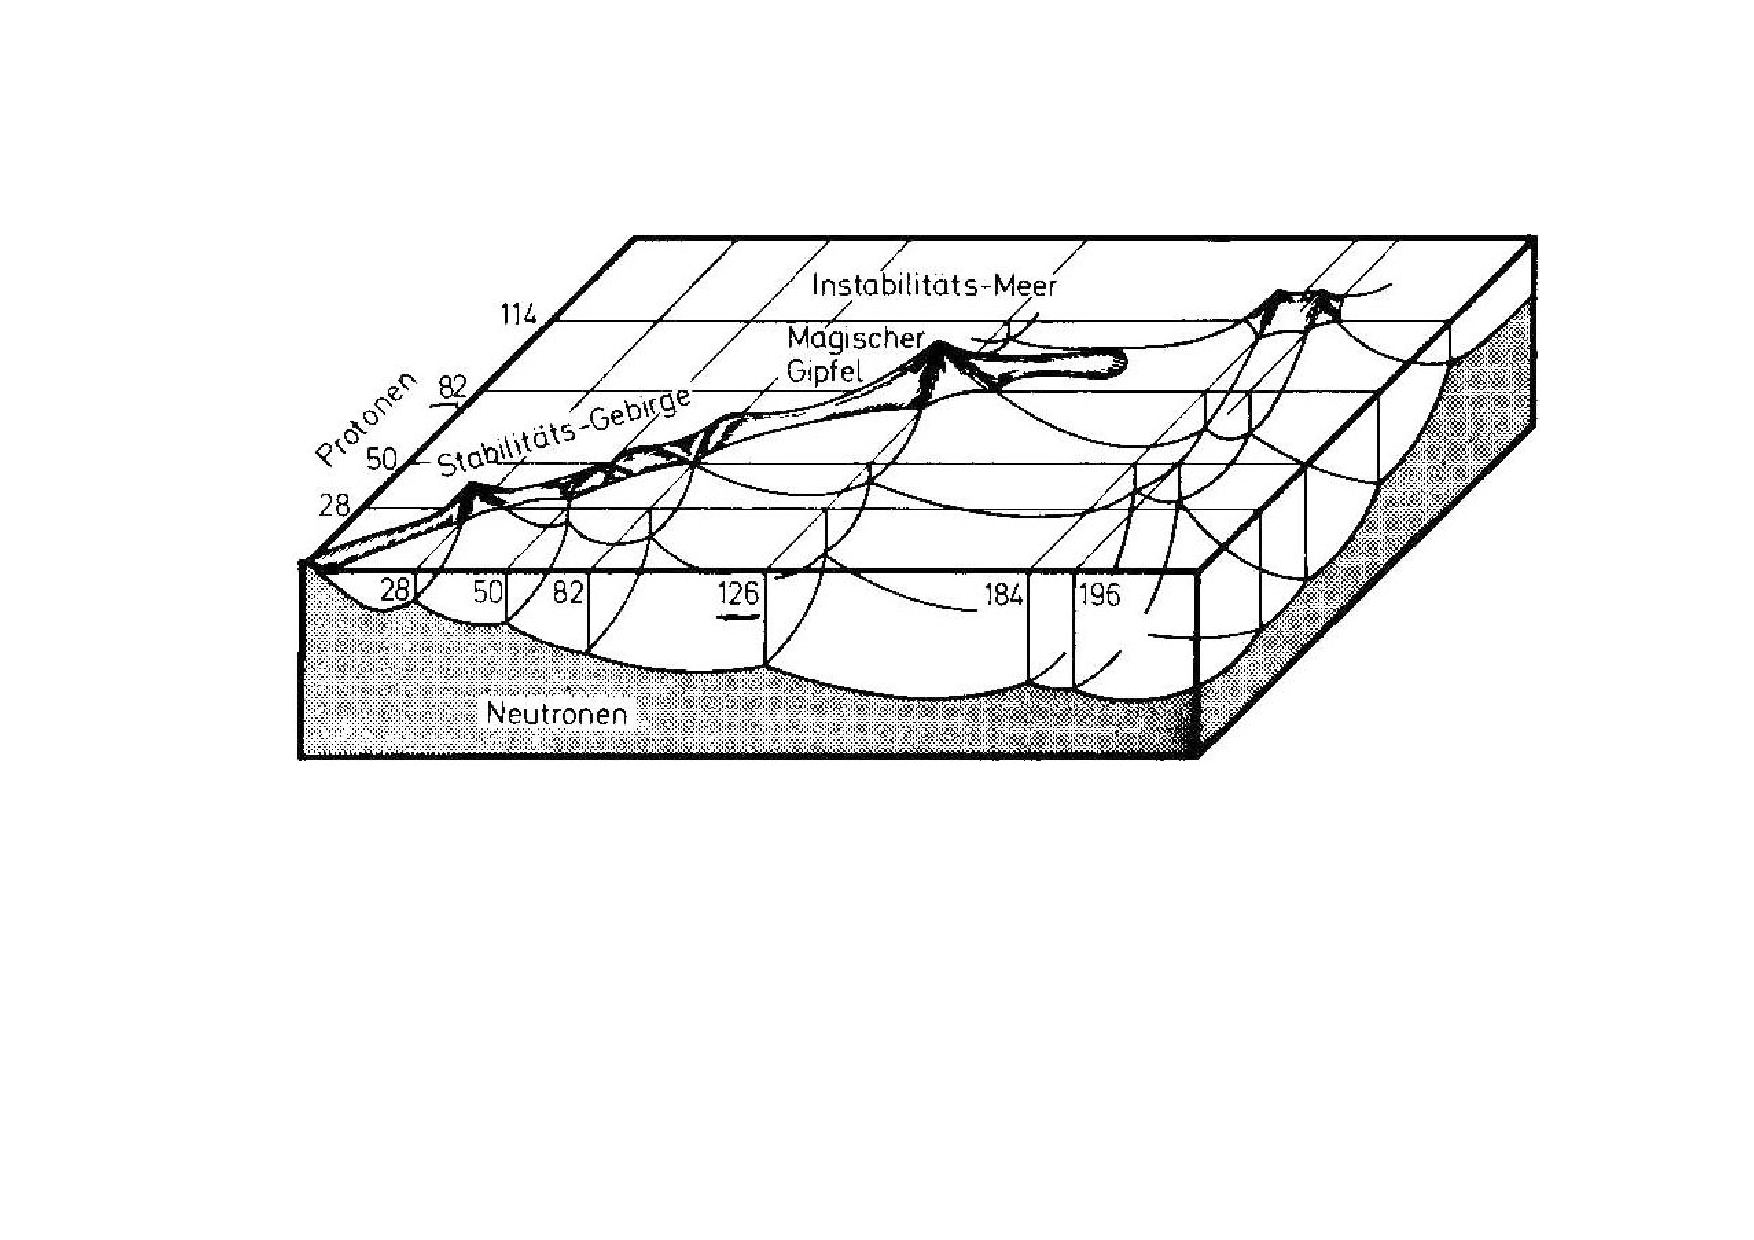
\includegraphics[width=\textwidth]{fig/2-StabilitaetsGebirge.pdf}
	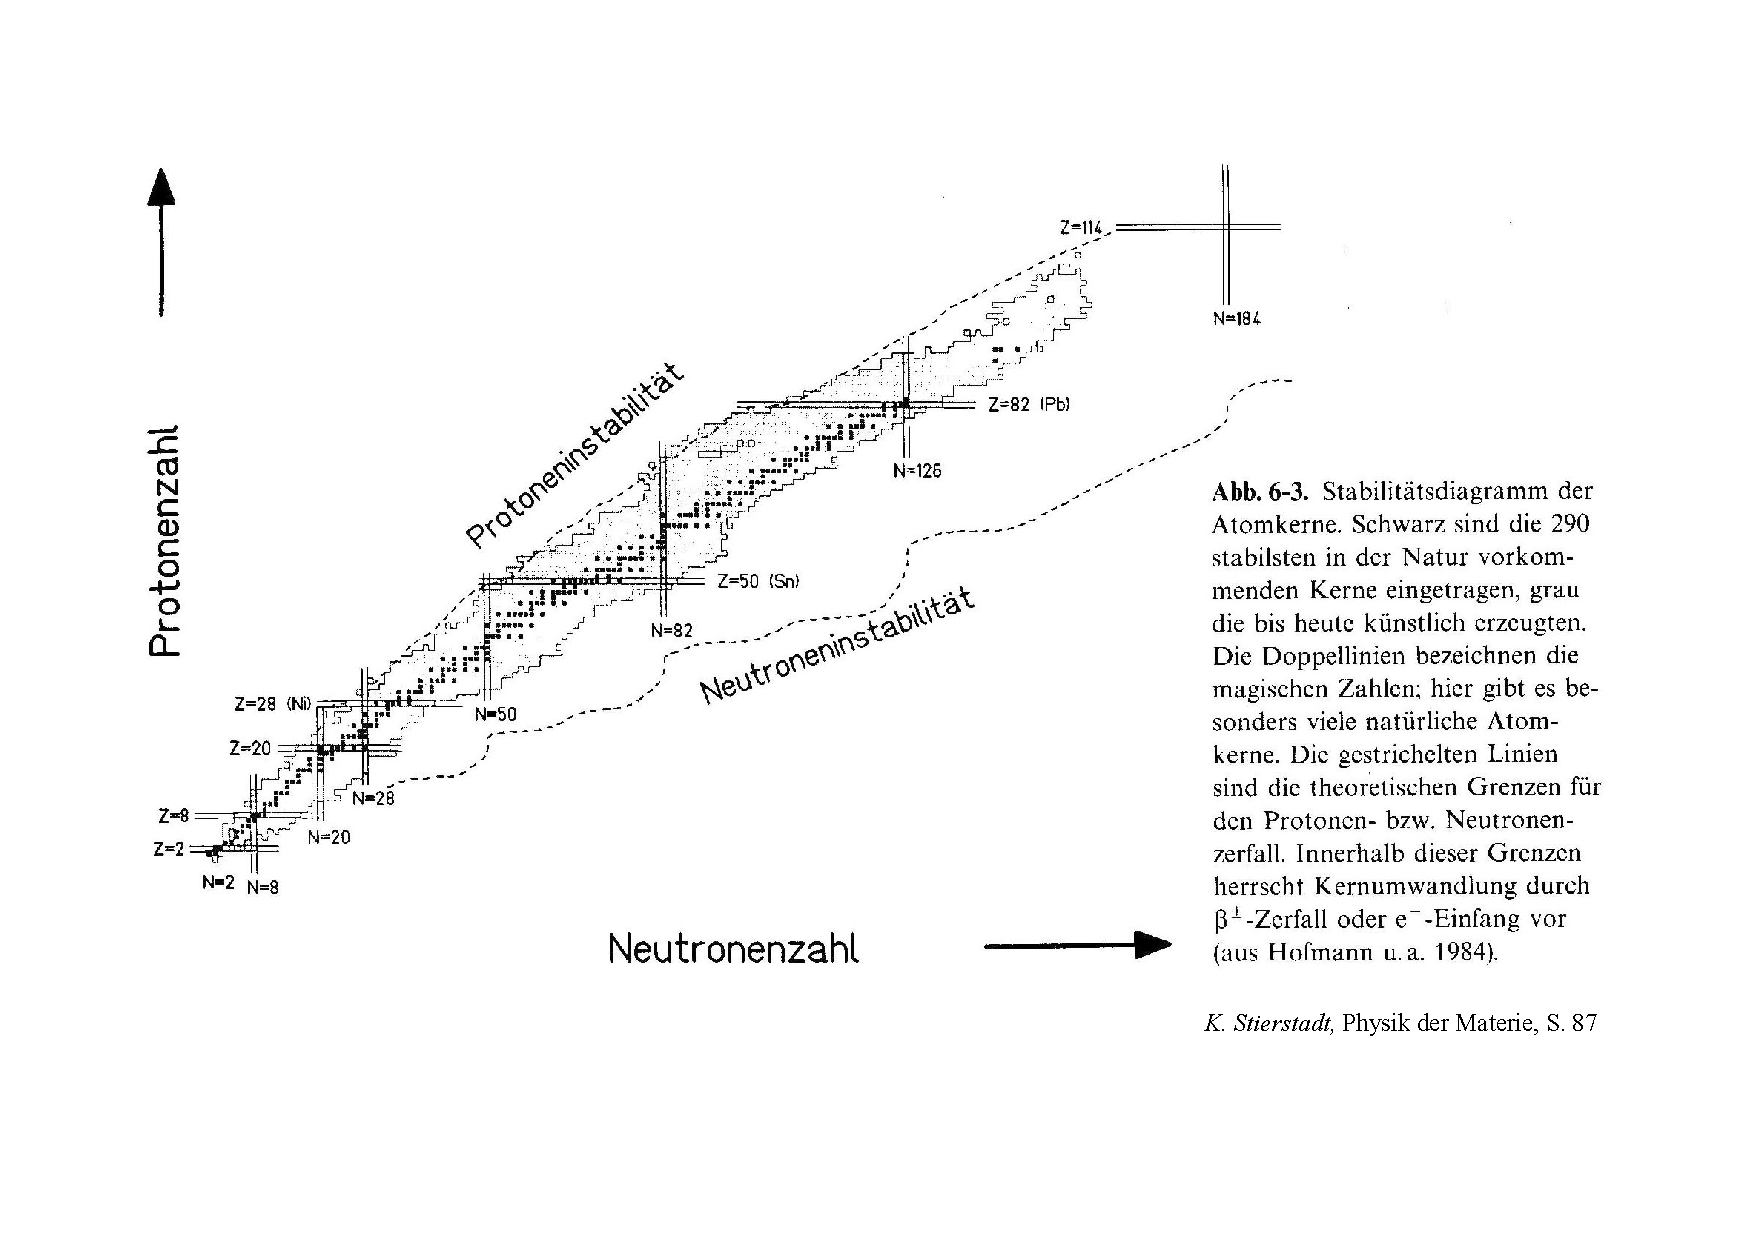
\includegraphics[width=\textwidth]{fig/2-Stabilitaetsdiagramm.pdf}
\end{figure}
\end{enumerate}
%\end{bemn}

\subsubsection{Kernreaktionen}

Wir wollen nun die Bethe-Weizsäcker Formel verwenden, um Aussagen über mögliche
Kernrekationen zu machen. Betrachten wir zunächst den $\alpha$-Zerfall. Die
Energie des $\alpha$-Zerfalls ist
\begin{align*}
E_\alpha =\frac{1}{c^2}
(m(Z,A)-\underbrace{m(Z-2,A-4)-m_\alpha}_{\small\text{Restkern +
$\alpha$ Teilchen}}).
\end{align*}
Falls $E_\alpha < 0$ wird die Teilchenwelle an den Potentialwänden
total reflektiert, durch Interferenz entstehen stehende Wellen. Dies sind
gerade die Eigenzustände des $\alpha$-Teilchens im Potential.

Ist $E_\alpha > 0$ im Potential, so existiert auch ein freier Zustand.
Die Welle wird nun nicht mehr total reflektiert, sondern dringt in die
Potentialwand ein und wird gedämpft. Wir wissen aus der Quantenmechanik,
dass daher das Teilchen eine gewisse Wahrscheinlichkeit hat, die
Potentialbarriere zu überwinden. Die Wahrscheinlichkeit für das Tunneln ist
gegeben durch,
\begin{align*}
&\lambda := \lambda_0\cdot T_\alpha,
\end{align*}
$\lambda_0$ ist die Entstehungswahrscheinlichkeit für das
$\alpha$-Teilchen, $T_\alpha$ bezeichnet den Transmissionskoeffizient.
\begin{align*}
T_\alpha &= \frac{\text{Zahl der erfolgreichen Eindringversuche}}{\text{Zahl
der gesamten Eindringversuche}}\\
&\entspr \text{Verhältnis von einlaufender zu auslaufender Teilchenwelle}.
\end{align*}
Betrachten wir die Wellenfunktionen der einlaufenden und auslaufenden Welle,
können wir den Transmissionkoeffizienten berechnen.
\begin{align*}
T_\alpha = \frac{j_a}{j_e} = \frac{\abs{\Psi_a}^2v_a}{\abs{\Psi_e}^2v_e}.
\end{align*}
Mit $p=mv = \hbar k$ und der Lösung der Wellengleichung für stehende
Wellen
\begin{align*}
\Psi_\nu = \alpha_\nu e^{ik_\nu x} + \beta_n e^{-ik_\nu x},
\end{align*}
erhält man so für das Kastenpotential,
\begin{align*}
T_\alpha = \exp\setd{-\frac{2}{\hbar}\int\limits_0^D \sqrt{2m(V(r)-E)}\dr}.
\end{align*}
Man kann zeigen, dass $T_\alpha$ für beliebige Potentiale diese Form hat.

\subsection{Zerfälle und Radioaktivität}

Über das zeitliche Verhalten von Kernreaktionen lassen sich folgende Aussagen
machen.
\begin{itemize}
  \item Der Zeitpunkt eines Zerfalls kann weder vorhergesagt noch von
  außen beeinflusst werden.
  \item Zerfälle werden durch die Wechselwirkung zwischen den Nukliden
  getrieben.
\end{itemize}
Man kann also nur Aussagen statistischer Natur machen. Wir wollen dies mit
Hilfe von Ratengleichungen tun. Dazu betrachten wir, wie sich eine große
Anzahl $N_0=N(t=0)$ von instabilen Kernen über die Zeit verändert. Sie erfüllt
die Differentialgleichung
\begin{align*}
\frac{\dN}{\dt} = -\Gamma N(t),
\end{align*}
wobei $\Gamma$ die \emph{Zerfallsrate} bezeichnet. Die Lösung dieser Gleichung
ist wohlbekannt,
\begin{align*}
N(t) = N_0 \exp\left(-\Gamma t\right).
\end{align*}
Die \emph{Aktivität} ist definiert als die Anzahl der Ereignisse pro Zeit,
\begin{align*}
A(t) = \abs{\frac{\dN}{\dt}} = N_0 \Gamma \exp\left(-\Gamma t\right).
\end{align*}
Die Aktivität hat also das gleiche Zeitverhalten wie die Anzahl der vorhandenen
Kerne. \textit{A posteriori} scheint dies offensichtlich, dass dem so ist, ist
jedoch eine Besonderheit und im Voraus nicht klar. Aus diesem Zusammenhang kann
man Informationen darüber gewinnen, wie sich die Radioaktivität zeitlich
verhält. Die Einheit der Aktivität ist die SI-Einheit,
\begin{align*}
1 \text{ Becquerel} = 1\mathrm{Bq}.
\end{align*}
\begin{bemn}
Die Aktivität sagt nichts über die Art der Strahlung, deren Energie oder deren
Schädlichkeit für Lebewesen aus.\maphere 
\end{bemn}
Die \emph{mittlere Lebensdauer} eines Kerns erhält man durch,
\begin{align*}
\tau = \frac{\int t\dN}{\int \dN} = \frac{\int t N_0 \Gamma \exp\left(-\Gamma
t\right)\dt}{N_0} = \frac{1}{\Gamma}.
\end{align*}
Die \emph{Halbwertszeit} ist die Zeit, nach der durchschnittlich die Hälfte der
vorhanden Kerne zerfallen ist,
\begin{align*}
&\frac{1}{2} N_0 = N_0 \exp\left(-\Gamma \tau_{1/2}\right)\\
\Leftrightarrow & \ln 2 = \Gamma \tau_{1/2}\\ 
\Leftrightarrow & \tau_{1/2} = \frac{\ln2}{\Gamma}
\end{align*}

In vielen Fällen ist nicht nur ein Zerfall möglich, man spricht dann von
``Zerfallskanälen''. Für ein Nuklid mit 2 Zerfallskanälen gilt,
\begin{align*}
\frac{\dN}{\dt}(t) = -\Gamma_1 N(t) - \Gamma_2 N(t) = -(\Gamma_1+\Gamma_2)N(t).
\end{align*}
Die Gesamtzerfallsrate ist $\Gamma_\text{ges} = \Gamma_1+\Gamma_2$,
Zerfallsraten sind also additiv. Die Halbwertszeit ergibt sich als
\begin{align*}
\tau = \frac{1}{\Gamma_\text{ges}} = \frac{1}{\Gamma_1+\Gamma_2}.
\end{align*}
Die Zeitabhängigkeit der Endprodukte ist
\begin{align*}
&\frac{\dN_i}{\dt} = -\Gamma_i N_i(t),\\
&\frac{N_1(t)}{N_2(t)} = \frac{\Gamma_1}{\Gamma_2}
\end{align*}
Lösungen dieser Gleichungen sind,
\begin{align*}
&N_1(t) = N_0 \frac{\Gamma_1}{\Gamma_1+\Gamma_2}\left(1 -
\exp\left(-\Gamma_\text{ges} t \right)\right)\\
&N_2(t) = N_0 \frac{\Gamma_2}{\Gamma_1+\Gamma_2}\left(1 -
\exp\left(-\Gamma_\text{ges} t \right)\right)
\end{align*}

% 
% \begin{figure}[!htbp]
% 	\centering
% 	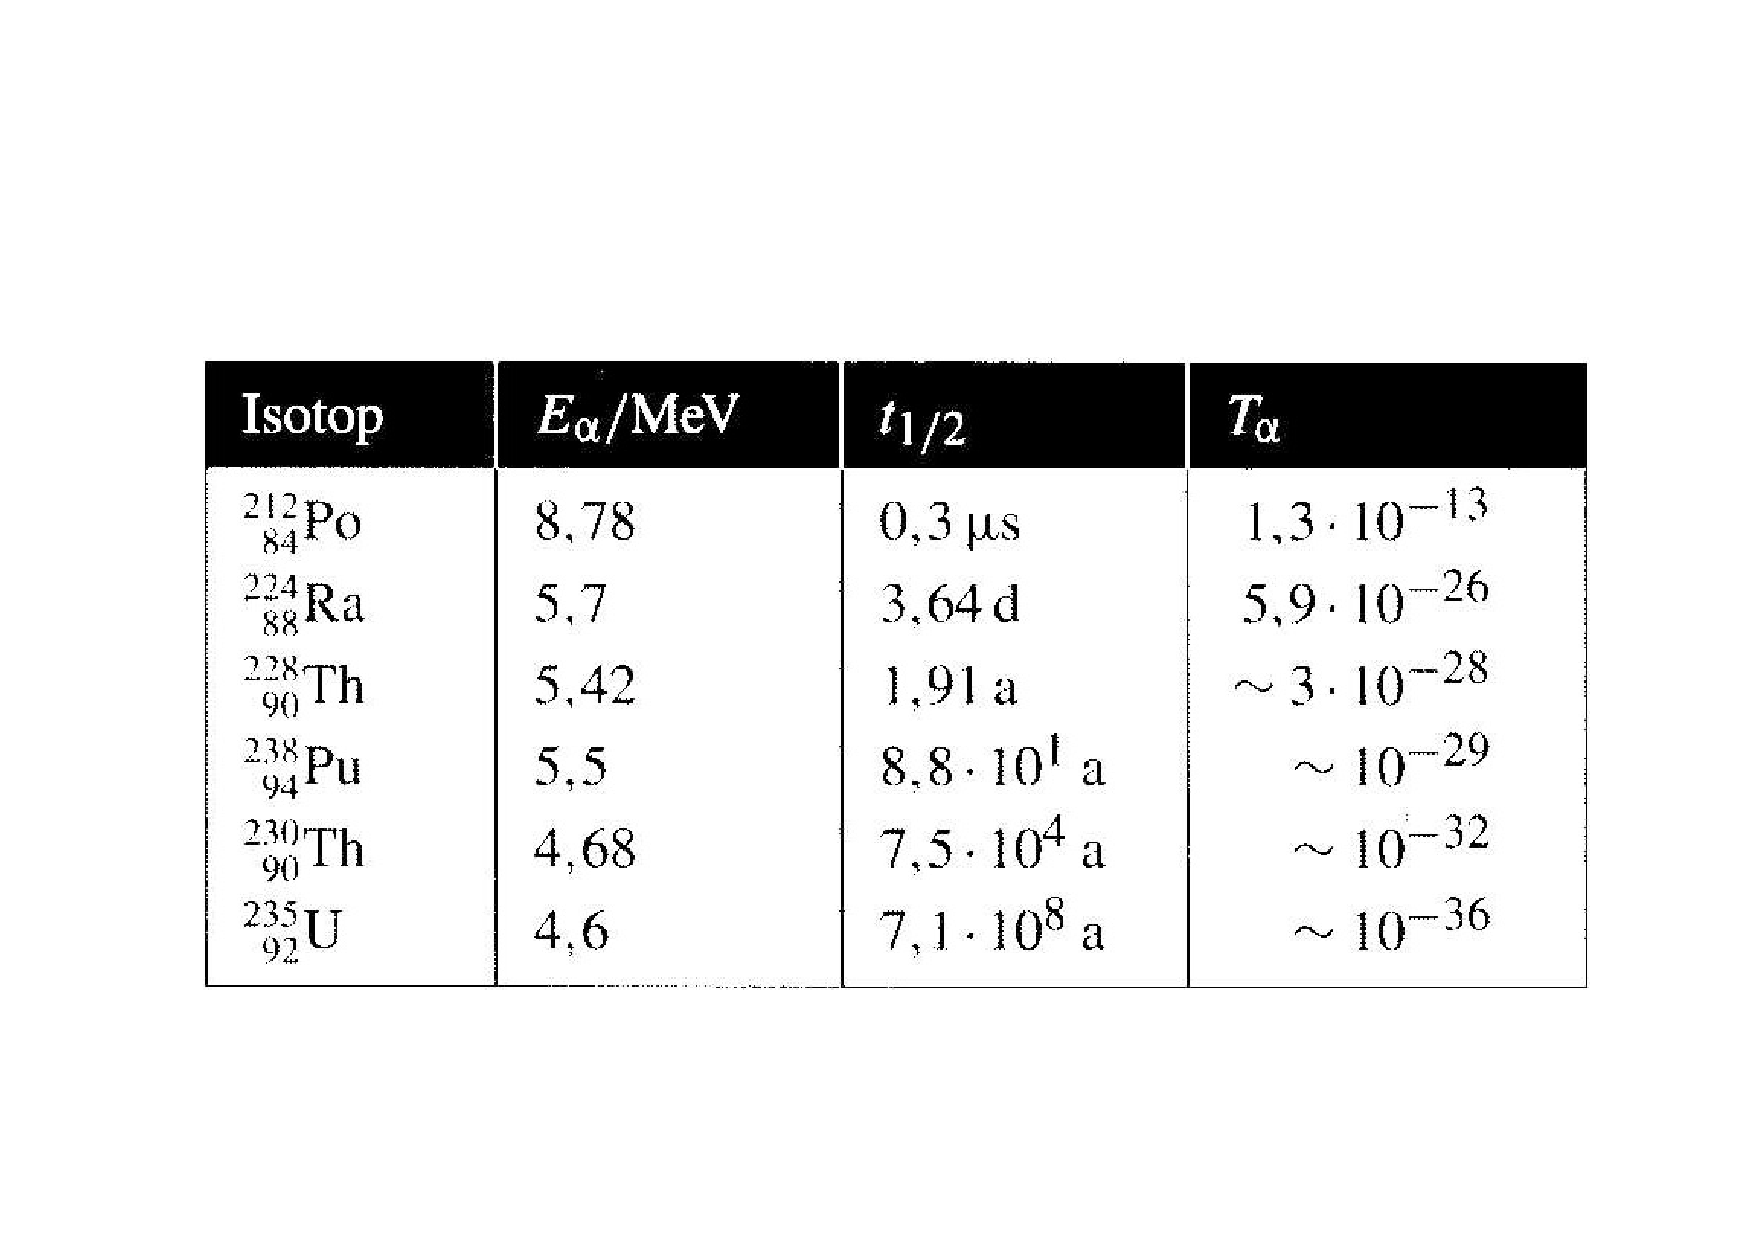
\includegraphics[width=0.9\textwidth]{fig/2-CharakteristischeDatenStrahler.pdf}
% \end{figure}

\sfigure[H][0.9]%
	{2-CharakteristischeDatenStrahler.pdf}
	{\DemtroederFour, S. 46}
	{Charakteristische Daten einiger $\alpha$-Strahler. (Energie $E_\alpha$,
	Halbwertszeit $t_{1/2}$ und Tunnelwahrscheinlichkeit $T_\alpha$)}

\subsubsection{Zusammenfassung}

\textit{$\alpha$-Strahlung} hat ein diskretes Spektrum, da die Anregungszustände
der Kerne diskret sind. Sie tritt dann auf, wenn durch die Abspaltung eines
$\alpha$-Teilchens die Bindungsenergie vergrößert werden kann. Da das
$\alpha$-Teilchen eine sehr hohe Bindungsenergie hat, wird dieser Zerfall
gegenüber der Abspaltung von einzelnen $p^+$, $n^0$ bevorzugt.

\textit{$\beta$-Strahlung} hat ein kontinuierliches Spektrum. Es handelt sich
hier um einen 3-Körper-Prozess, weshalb die Energie kontinuierlich verteilt
werden kann.
\begin{align*}
&n^0 \to p^+ + e^- + \overline{\nu}_e\\
&p^+ \to n^0 + e^+ + \nu_e
\end{align*}
Beim Zerfall entstehen die Spin-$\frac{1}{2}$-Teilchen Elektronneutrino $\nu_e$
bzw. Elektronantineutrino $\overline{\nu}_e$ aufgrund der
Impuls- und Drehimpulserhaltung.

\textit{$\gamma$-Strahlung} entsteht bei ``optischen Übergängen'' von
angeregten Kernzuständen. Hierbei werden Photonen im $\mathrm{MeV}$-Bereich
emittiert. Typischerweise folgt auf einen $\alpha$-/$\beta$-Zerfall ein
$\gamma$-Zerfall, da die Zerfallsprodukte bei letzteren in angeregten
Zuständen zurückbleiben.

Aus der Paritätsregel und der Drehimpulserhaltung erhalten wir Auswahlregeln
für diese Übergänge. Dipolstrahlung im Fall von $\Delta L = 1$,
Quadrupolstrahlung für $\Delta L = 2$.

\subsubsection{Andere Strahlungseinheiten}
Wird ein lebender Organismus Strahlung ausgesetzt, kann man mithilfe der
\emph{Dosis} Aussagen über die Auswirkungen machen,
\begin{align*}
&\nrm{D} = \nrm{\frac{\text{absorbierte Energie}}{\text{Masse}}} = 1
\frac{\mathrm{J}}{\mathrm{kg}} = 1 \mathrm{Gray} = 1 \mathrm{Gy}\\
&\nrm{\dot{D}} = \frac{\mathrm{Gy}}{\mathrm{s}}.
\end{align*}
Die Schädlichkeit der Strahlung an sich wird durch die \emph{Äquivalentdosis}
\begin{align*}
H=Q\cdot D,\qquad \text{Einheit }S_V\text{ (Sievert)},
\end{align*}
beschrieben, wobei $Q$ einen Qualitätsfaktor darstellt.

%\begin{table}[h]
\begin{tabular}[h]{l|c}
 & $Q$\\\hline
 $\gamma/\beta$-Strahlung & 1\\
 thermische Neturonen $n_\tau$ & 2.3\\
 schnelle Neutronen $n_S$ & 10\\
 $\alpha$-Strahlung & 20
\end{tabular}
%\end{table}


\newpage
\section{Atome}

Während die beobachteten Wellenlängen in der Kernphysik im Bereich der
$\gamma$-Strahlung liegen, sind die der Atomphysik im sichtbaren Bereich. Bei
den Längenskalen verhält es sich ähnlich,
\begin{align*}
&\mathrm{fm},\qquad\text{Kernphysik},\\
&\mathrm{\AA},\qquad\text{Atomphysik},\qquad \AA = 10^{-10}m.
\end{align*}

Schon in der Antike hatte man die Idee, dass die Materie aus kleinsten
Teilchen, den Atomen, aufgebaut ist. Als einer der ersten formulierte
Bernouli\footnote{Daniel Bernoulli (* 8. Februar 1700 in Groningen; † 17. März
1782 in Basel)  war ein Schweizer Mathematiker und Physiker aus der
Gelehrtenfamilie Bernoulli.} gegen Ende des 18. Jahrhunderts die Hypothese, dass Materie  aus kleinsten Teilchen bestehe, welche wechselwirken und sich
gegenseitig abstoßen. 1869 veröffentlichte Mendelejew\footnote{Dmitri
Iwanowitsch Mendelejew (* 8. Februar 1834 in Tobolsk, Russland; † 20.
2. Februar 1907 in Sankt Petersburg) war ein russischer Chemiker.} eine erste
Version des Periodensystems der Elemente.

In diesem Kapitel wollen wir untersuchen, welche Kräfte zwischen den
Bestandteilen der Atome wirken und durch welche Potentiale sie sich beschreiben
lassen, um ein Modell zu entwickeln, das es uns ermöglicht, die Struktur des
Periodensystems der Elemente zu erklären.
\begin{bspn}
Folgendes Experiment Anfang des 20. Jahrhunderts zeigte Phänomene, die mit der
damaligen Physik nicht zu erklären waren.

\begin{figure}[!htbp]
	\centering
	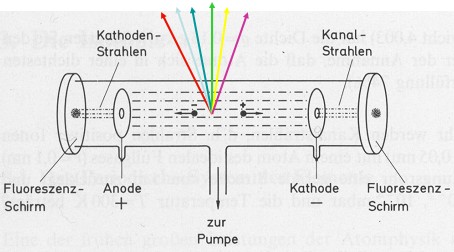
\includegraphics[width=\textwidth]{fig/3-SpektroskopieGasentladung.png}
	\caption{Spektroskopie von Gasentladungen}
\end{figure}

Man bringt in eine Gasröhre Elektroden ein, an die man eine hohe Spannung
anlegt. Es kommt zur Gasentladung, ein Lichtbogen wird beobachtet.
Spektroskopiert man den Lichtbogen, wird kein kontinuierliches Spektrum
festgestellt, sondern lediglich wenige diskrete Frequenzen.\bsphere
\end{bspn}

%TODO: Experiment Reflexion am Gitter
%TODO: Experiment Absorptionsspektroskopie
%TODO: Experiment Laserspektroskopie, Lösung des Dopplereffekts

Bei Spektroskopie steht die Frequenzmessung im Mittelpunkt. Die Präzession
dieser Messung ist heute auch im optischen Frequenzbereich so groß, dass man
mithilfe von optischen Frequenzmessungen Uhren bauen kann, die Zeit so exakt
messen, wie Cäsium Uhren, welche ebenfalls auf einer Mikrowellenfrequenzmessung
basiert. Es wird daher diskutiert, ob die Definition der Sekunde durch eine
optische Übergangsfrequenz gegeben werden soll.

 \begin{figure}[!htbp]
	\centering
	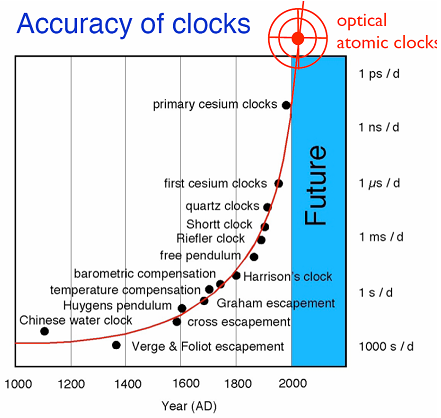
\includegraphics[width=\textwidth]{fig/3-AccuracyOfClocks.png}
	\caption{Präzission von Atomuhren.}
\end{figure}

Die Frequenz ist aber auch im Alltag eine sehr wichtige Messgröße.
\begin{bspn}
GPS basiert auf Längenmessungen, die man durch Laufzeitmessungen der GPS
Signale realisiert,
\begin{align*}
s = v\cdot t = c\cdot\frac{1}{f}.
\end{align*}
Je genauer die Frequenz bestimmt ist, desto genauer ist die
Positionsbestimmung.\bsphere
\end{bspn}


\subsection{Bohr'sches Atommodell}

Niels Bohr\footnote{Niels Henrik David Bohr (* 7. Oktober 1885 in Kopenhagen; †
18. November 1962 in Kopenhagen) war ein dänischer Physiker und
Nobelpreisträger für Physik des Jahres 1922} stellte 1913 erstmals
das später nach ihm benannte Atommodell vor.

Er suchte nach Erklärungen für den experimentellen Befund, dass
Atomspektren aus diskreten Linien bestehen.

Im sichtbaren Bereich kannte man die Balmer-Serie\footnote{Johann Jakob Balmer
(* 1. Mai 1825 in Lausen, Kanton Basel-Landschaft; † 12. März 1898 in Basel)
war ein Schweizer Mathematiker und Physiker.} (1885, $n'=2$) mit,
\begin{align*}
&\lambda = \frac{n^2}{n^2-2^2}G,\qquad m>2,\ B=364.56\mathrm{nm}\\
&\overline{\nu} = \frac{1}{\lambda} = R\left(\frac{1}{2^2}-\frac{1}{n^2}
\right),
\end{align*}
wobei $\overline{\nu}$ die \emph{Wellenzahl} und $R$ die empirisch bestimmte
\emph{Rydbergkonstante} bezeichnen. Im Ultravioletten die
Lyman-Serie\footnote{Theodore Lyman (* 23. November 1874 in Boston,
Massachusetts; † 11. Oktober 1954 in Cambridge, Massachusetts) war ein
amerikanischer Physiker.} (1906, $n'=1$), im Infraroten die
Paschen-Serie\footnote{Friedrich Paschen (* 22. Januar 1865 in Schwerin; † 25.
Februar 1947 in Potsdam) war ein deutscher Physiker, der 1921 gemeinsam mit
Ernst Back den Paschen-Back-Effekt entdeckte.} (1908, $n'=3$) und die
Brackett-Serie\footnote{Frederick Sumner Brackett (* 1. August 1896 in
Claremont, California; † 28. Januar 1988) war ein US-amerikanischer Physiker
und Spektroskopiker.} (1923, $n'=4$). \begin{figure}[!htbp]
	\centering
	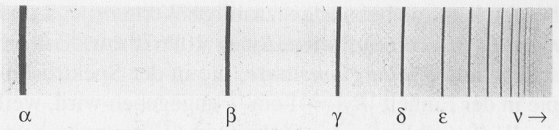
\includegraphics[width=\textwidth]{fig/3-BalmerSerie.png}
	\caption{Balmer Serie 1885}
\end{figure}

Als empirisches Ergebnis wurde 1913 von Rydberg\footnote{Johannes Robert
Rydberg (* 8. November 1854 in Halmstad; † 28. Dezember 1919 in Lund) auch
bekannt als Janne Rydberg, war ein schwedischer Physiker.} postuliert,
\begin{align*}
\overline{\nu} = R\left(\frac{1}{{n'}^2}-\frac{1}{n^2}\right),\quad n'<n\in\N.
\end{align*}

Bohr kannte bereits das Rutherford'sche Atommodell, bei dem ein Elektron um den
Kern in der Mitte kreist. Die Elektrodynamik verlangt jedoch, dass das auf die
Kreisbahn gezwungene Elektron kontinuierlich Energie abstrahlt und somit
zwangsläufig in den Kern stürzt.
%TODO: Skizze Spiralbahn

Um dieses Problem zu lösen, stellte Bohr folgende Postulate auf.
\begin{enumerate}[label=\arabic{*})]
  \item Das Atom ähnelt einem Planetensystem (Rutherford), bei dem die
  Elektronen um den Kern kreisen.
  \item Die Coulomb-Wechselwirkung zwischen Kern und Elektron und die 
  Zentrifugalkraft kompensieren sich.
  \item Es sind nur bestimmte Energieniveaus zulässig.
  \item Die Bewegung der Elektronen erfolgt strahlungslos.
  \item Die Elektronen können jedoch zwischen den erlaubten Energieniveaus
  springen und emittieren dabei Photonen mit
\begin{align*}
\nu = \frac{\Delta E}{h} = \frac{E_n-E_{n'}}{h},\quad \text{Planck (1900)}.
\end{align*}
\item \textit{Korrespondenzprinzip}. Für große $n$, also große Bahnradien,
sollen die klassischen Gesetze gelten.
\end{enumerate}

\begin{figure}[!htbp]
	\centering
	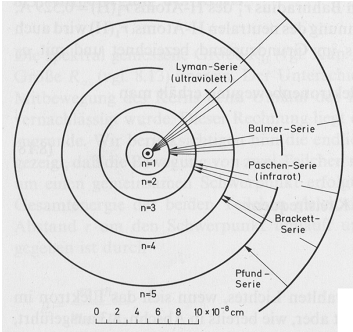
\includegraphics[width=\textwidth]{fig/3-BohrscherWasserstoff.png}
\end{figure}


Wir wollen diese Postulate nun mathematisch erfassen. Zentripetal- und
Coulombkraft sind im Gleichgewicht,
\begin{align*}
&F_{\text{Coulomb}} = -\frac{1}{4\pi\ep_0}\frac{Ze^2}{r^2},\quad
F_{\text{Zentripetal}} = mr\omega^2\\
&F_{\text{Zentripetal}}+F_{\text{Coulomb}} = 0.
\end{align*}
Dies ergibt eine Kreisbahn für das Elektron mit,
\begin{align*}
&\frac{1}{4\pi\ep_0}\frac{Ze^2}{r^2} = mr\omega^2\tag{1}\\
\Rightarrow\;&r(\omega) =
\left(\frac{1}{4\pi\ep_0}\frac{Ze^2}{m\omega^2}\right)^{1/3}\tag{2}.
\end{align*}
Betrachtet man nun die Energiewerte,
\begin{align*}
&E = E_{\text{kin}} + E_{\text{pot}}\\
&E_{\text{kin}} = \frac{1}{2}mv^2 = \frac{1}{2}mr^2\omega^2\\
&E_{\text{pot}} = \frac{1}{4\pi\ep_0}\int\limits_{\infty}^r
\frac{Ze^2}{{r'}^2}\dr' = -\frac{1}{4\pi\ep_0}\frac{Ze^2}{r}\\
\Rightarrow & E = \frac{1}{2}mr^2\omega^2 - \frac{1}{4\pi\ep_0}\frac{Ze^2}{r}
\end{align*}
Setzen wir nun unsere Ausdrücke für $E_{\text{pot}}$ und $r(\omega)$ ein,
\begin{align*}
\overset{(1)}{\Leftrightarrow} & E = \frac{1}{2}mr^2\omega^2 - mr^2\omega^2 =
-\frac{1}{2}mr^2\omega^2 \overset{(2)}{=}
-\frac{1}{2}m\left(\frac{1}{4\pi\ep_0}\frac{Ze^2}{m\omega^2}\right)^{2/3}\omega^2\\
&\quad 
= -\frac{1}{2}\left(\frac{1}{(4\pi\ep_0)^2}m\omega^2Z^2e^4\right)^{1/3},\tag{3}
\end{align*}
und verwenden Bohrs Postulat der diskreten Energieniveaus,
\begin{align*}
&E_n = -R\frac{hc}{n^2},\qquad n,n'=1,2,3,\ldots\text{ Quantenzahlen}\\
&E_{n'} = -R\frac{hc}{{n'}^2},\\
\Rightarrow & \Delta E = E_n-E_{n'} =
Rhc\left(\frac{1}{{n'}^2}-\frac{1}{n^2}\right).
\end{align*}
Das Modell erklärt somit das empirische Ergebnis,
\begin{align*}
\nu = \frac{\Delta E}{h} = Rc\left(\frac{1}{{n'}^2}-\frac{1}{n^2}\right),\quad
\nu = c\overline{\nu}.
\end{align*}
Betrachten wir $\Delta E$ für $n-n'=1$, so ergibt sich,
\begin{align*}
\nu = Rc\left(\frac{1}{(n-1)^2}-\frac{1}{n^2}\right) = 
Rc\frac{1}{n^2}\left(\frac{1}{\left(1-\frac{1}{n}\right)^2}-1\right).\tag{4}
\end{align*}
Für die Eigenenergien erhalten wir die Beziehung,
\begin{align*}
E_n = -\frac{1}{2}\left(\frac{1}{(4\pi\ep_0)^2}Z^2e^4m\omega^2\right)^{1/3} =
-\frac{Rhc}{n^2}.\tag{5}
\end{align*}
Klassisch erwarten wir so (Auflösen von (5) nach $\omega$),
\begin{align*}
\nu_{\text{klass.}} = \frac{\omega}{2\pi} \sim \frac{1}{n^3}.
\end{align*}
In Gleichung (4) haben wir jedoch $\sim\frac{1}{n^2}$.

Beachten wir, dass Bohrs Postulate nur für große $n$ eine Übereinstimmung
besagen, müssen wir den zweiten Faktor in (4) entwickeln,
\begin{align*} 
\frac{1}{\left(1-\frac{1}{n}\right)^2}
\approx 1 + \frac{2}{n} + \frac{3}{n^2}+\ldots
\end{align*}
Wenden wir diese Entwicklung in (4) an, so ergibt sich
\begin{align*}
\nu = Rc\frac{2}{n^3},\tag{6}
\end{align*}
was wieder mit der klassischen Erwartung übereinstimmt.

Wir wollen nun diesen Zusammenhang nutzen, um die Rydbergkonstante $R$ konkret
zu berechnen,
\begin{align*}
&\frac{Rhc}{n^2} = \frac{1}{2}\left(\frac{1}{(4\pi\ep_0)^2}Z^2e^4m\omega^2
\right)^{1/3} \overset{(6)}{=}
\frac{1}{2}\left(\frac{1}{(4\pi\ep_0)^2}Z^2e^4m\left(2\pi \frac{2Rc}{n^3}\right)^2
\right)^{1/3}.
\end{align*}
Für Wasserstoff erhalten wir so den Wert,
\begin{align*}
R = \frac{me^4}{8\ep_0^2 h^3 c}.\tag{7}
\end{align*}
Für Messung und Rechnung ergibt sich der Unterschied,
\begin{align*}
&R_{\text{Messung}} = (109737.318\pm 0.012)\mathrm{cm^{-1}},\\
&R_{\text{Rechnung}} = (109677.581)\mathrm{cm^{-1}}.
\end{align*}
Wir sehen, dass die Rechnung eine große Übereinstimmung mit den experimentellen
Daten hat.

Später werden wir diese Vorhersage noch verbessern, indem wir mit der
reduzierten Masse rechnen, da der Kern nicht - wie angenommen - unendlich
schwer ist und sich in Ruhe befindet, sondern sich mitbewegt.

\begin{bspn}
Der Bohrradius der ``kleinsten Bahn'' ($n=1$) im Wasserstoff-Atom ist
\begin{align*}
a_0 = 0.529 \AA,\qquad \AA = 10^{-10}\mathrm{m}.\bsphere
\end{align*}
\end{bspn}

Betrachten wir den Drehimpuls $\vec{l} = \vec{r}\times\vec{p}$ im Bohr'schen
Atommodell des Wasserstoffatoms, so ergibt sich,
\begin{align*}
\abs{\vec{l}} &= mr_n^2\omega_n \overset{(2)}{=}
m\left(\frac{1}{4\pi\ep_0}\frac{e^2}{m\omega_n^2}\right)^{2/3}\omega_n\\
&\overset{(6)}{=} m\left(\frac{1}{4\pi\ep_0}\frac{e^2}{m}\right)^{2/3}
\left(\frac{n^3}{4\pi R c}\right)^{1/3}
=\left(\frac{1}{(2\pi)^3}\frac{me^4}{8\ep_0^2h^3c}\frac{1}{R} \right)^{1/3}nh
 \\
&= n\hbar.
\end{align*}
Der Drehimpuls steigt also linear mit der Hauptquantenzahl an. Im Grundzustand
($n=1$) ist $\abs{\vec{l}}=\hbar$.
\begin{bemn}
Bohr und Sommerfeld haben diese Erkenntnisse genutzt, um eine allgemeine
Quantisierungsbedingung für geschlossene Bahnen aufzustellen,
\begin{align*}
\oint \vec{p} \dvecr =n h,
\end{align*}
die \emph{Bohr-Sommerfeldsche-Quantisierungsmethode}.
Ausgehend von dieser Quantisierung lassen sich andere Größen besonders
geschickt quantisieren. In Potentialen mit geschlossenen Bahnkurven ist
dies daher eine sehr gute Grundlage.
Dennoch hat sie ihre Grenzen. Das freie Teilchen wird beispielsweise von dieser
Methode nicht erfasst, da es keine geschlossene Bahnkurve besitzt. Später werden wir diese,
heute als antiquiert geltende Methode, durch die Schrödingergleichung ersetzen, 
mit der uns ein allgemeiner Ansatz für beliebige Potentiale zur Verfügung
steht.\maphere
\end{bemn}

Für die Umlauffrequenz erhalten wir den Wert,
\begin{align*}
\omega_n = \frac{4\pi Rc}{n^3} =
\frac{1}{(4\pi\ep_0)^2}\frac{Z^2e^4m}{\hbar^3n^3}.
\end{align*}
\begin{bspn}
Die Umlauffrequenz des Wasserstoffatoms im Grundzustand $(Z=1,n=1)$ ist
\begin{align*}
\omega(H) \approx 10^{16}\mathrm{s}^{-1}.\bsphere
\end{align*}
\end{bspn}

Die Geschwindigkeit des Elektrons auf der Bohrschen Bahn ist,
\begin{align*}
v = \omega_n r_n = Z\underbrace{\frac{e^2}{4\pi\ep_0\hbar
c}}_{\alpha}\frac{1}{n}c,\quad
\alpha\approx\frac{1}{137}\text{ heißt \emph{Feinstrukturkonstante}}.
\end{align*}
Die Geschwindigkeit ist zwar groß, beim Wasserstoffatom jedoch noch hinreichend
klein, um ohne relativistische Rechung auszukommen. Für größere Ordnungszahlen
muss man jedoch relativistische Effekte berücksichtigen.

Für Atome mit $Z\approx 137$ ist $v\approx c$ und das Modell bricht zusammen.
Die ``stationären Bahnen'' sind dann nicht mehr stationär, die Atome sind
nicht mehr stabil, sie zerfallen.

Die Bindungsenergie ist gegeben durch,
\begin{align*}
E_n = -\frac{Rhc}{n^2}= -\frac{1}{2}m\omega_n^2r_n^2 =
-\frac{Z^2e^4m}{32\pi^2\ep_0^2\hbar^2}\frac{1}{n^2}.
\end{align*}

\begin{bspn}
Für $Z=1,n=1$ erhalten wir
\begin{align*}
E_n = -13.6\mathrm{eV},
\end{align*}
was ebenfalls sehr gut mit der experimentellen Erfahrung übereinstimmt.\bsphere
\end{bspn}

\textit{1. Bewährungsprobe des Bohrschen Modells.}
\begin{align*}
\Delta R = R_{\text{exp}}-R_{\text{theo}} = -60\mathrm{cm^{-1}}\qquad
(H\text{-Atom})
\end{align*}
Wir wollen nun die Mitbewegung des Kerns berücksichtigen und rechnen mit der
reduzierten Masse,
\begin{align*}
\mu = \frac{m_em_{\text{Kern}}}{m_e+m_{\text{Kern}}}
= \frac{m_e}{1+\frac{m_e}{m_{\text{Kern}}}}
\end{align*}
%TODO: Bild Schwerpunktsystem
Die Rydbergkonstante errechnet sich somit durch,
\begin{align*}
R_\mu = \frac{\mu e^4}{8\ep_0^2 h^3c} =
\frac{1}{1+\frac{m_e}{m_{\text{Kern}}}}R_\infty.
\end{align*}
Als Abweichung vom gemessenen Wert der Rydbergkonstante erhalten wir nun,
\begin{align*}
\Delta R = -59\mathrm{cm^{-1}}\qquad (H\text{-Atom}),
\end{align*}
d.h. durch die Berücksichtigung der Mitbewegung des Kerns erhalten wir eine
etwas höhere Genauigkeit.

Als Anwendung können wir unter Annahme des Bohrschen Atommodells 
das Verhältnis von Protonen und Elektronenmasse bestimmen,
\begin{align*}
\frac{m_p}{m_e} = 1836.15,
\end{align*}
was ebenfalls sehr gut mit den massenspektrometrischen Messungen übereinstimmt.

Wenn wir vom Wasserstoff zum nächst schwereren Isotop dem Deuterium übergehen
(Isotopieverschiebung), ergibt sich
\begin{align*}
&R_H = 109677.581\mathrm{cm^{-1}},\\
&R_D = 109670.7\mathrm{cm^{-1}},
\end{align*}
in sehr guter Übereinstimmung mit den Messergebnissen.

\sfigure%
	{3-KorrekturMitbewegungKern.pdf}%
	{\HakenWolf, S. 110}%
	{Energiekorrektur wegen Mitbewegung des Kerns für die Rydberkonstante einiger
	Einelektronen Atome.}
% \begin{figure}[!htbp]
% 	\centering
% 	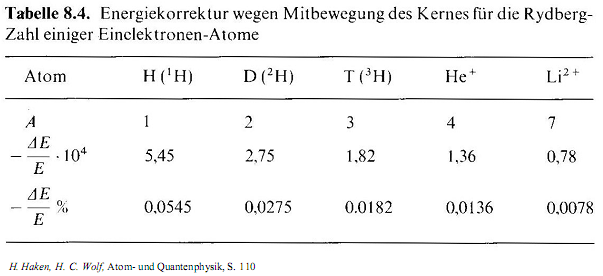
\includegraphics[width=\textwidth]{fig/3-KorrekturMitbewegungKern.png}
% \end{figure}

\textit{2. Bewährungsprobe des Bohrschen Modells.}

Für Atome mit höherer Ordnungszahl aber nur einem Elektron,
d.h. $He^+$, $Li^{++}$, $Be^{+++}$, usw. erhalten wir ein Wasserstoff ähnliches
Spektrum. Das Bohr-Sommerfeld-Modell sagt für die Bindungsenergie
\begin{align*}
E_n \sim \frac{Z^2}{n^2},
\end{align*}
voraus, d.h. sie steigt quadratisch mit $Z$ an. Auch dies lässt sich experimentell
bestätigen. Ein Extremfall in guter Übereinstimmung ist $U^{91+}$.

\subsubsection{Erweiterung des Bohr'schen Atommodells nach Sommerfeld}

Lässt man nicht nur Kreis- sondern auch Ellipsenbahnen zu, kann man das Modell
zum \emph{Bohr-Sommerfeld-Atommodell} erweitern. Die Ellipsengleichung ist
\begin{align*}
r = \frac{a(1-\ep^2)}{1+\ep\cos\ph},
\end{align*}
mit der goßen Halbachsen $a$ und der Exzentrität $\ep$.
\begin{figure}[!htpb]
\centering
\begin{pspicture}(0,-0.64)(2.4,0.64)
\psellipse(1.2,0.0)(1.2,0.64)
\psline(1.2,0.0)(1.2,0.62)
\psline(1.2,0.0)(2.38,0.0)

\rput(1.05,0.305){\color{gdarkgray}$b$}
\rput(1.82,-0.115){\color{gdarkgray}$a$}
\end{pspicture}\qquad
\begin{pspicture}(-0.2,-0.7)(2.2,0.6)
\pscircle(0.33,0.16){0.33}
\psellipse(1.55,0.14)(0.55,0.07)

\rput(0.31,-0.365){\color{gdarkgray}$\ep=0$}
\rput(1.53,-0.365){\color{gdarkgray}$\ep\to1$}
\end{pspicture} 
\caption{Ellipse mit großer Halbachse $a$ und kleiner Halbachse $b$ (links)
Einfluss der Exzentrität (rechts).}
\end{figure}
Eine Ellipsenbahn hat kleineren Drehimpuls als eine Kreisbahn.  Für $\ep=0$ 
erhalten wir den Kreis zurück, divergiert die Exzentrität $\ep\to1$, so
pendelt das Elektron durch den Kern $\Rightarrow l=0$.

Um dies herzuleiten, wählt man eine Bindungsenergie und eine
Quantisierungsbedingung und löst das Keplerproblem. Die Bindungsenergie ist
\begin{align*}
E_n = -\frac{Ze^2}{2a} = -\frac{Rhc}{n^2},
\end{align*}
hängt also nicht von $\ep$ ab. Es sind somit nicht nur Kreisbahnen als Lösungen
zugelassen sondern auch Ellipsen. Klassisch sind alle Bahnen mit $\ep\in[0,1)$
erlaubt, die quantenmechanische Behandlung nach Sommerfeld fordert jedoch,
\begin{align*}
&\oint p(r)\dr = n_r h,\\
&\oint p(\ph)\dph = n_\ph h.
\end{align*}
D.h. es sind nur diskrete $\ep$ erlaubt. Wir sehen wie in der Kernphysik, dass
für hohe Quantenzahlen, die Zustände zunehmend entarten, d.h. unterschiedliche
Zustände die gleiche Energie haben.

\begin{figure}[!htbp]
\centering
\begin{pspicture}(-0.5,-2.12)(4.2,2.3)
\psline{->}(0.74,-1.8)(0.74,2.08)
\psline(1.12,-1.6)(1.36,-1.6)
\psline(1.12,0.18)(1.36,0.18)
\psline(1.12,0.98)(1.36,0.98)
\psline(1.12,1.38)(1.36,1.38)
\psline(1.72,0.18)(1.96,0.18)
\psline(1.72,0.98)(1.96,0.98)
\psline(1.72,1.38)(1.96,1.38)
\psline(2.34,0.98)(2.58,0.98)
\psline(2.34,1.38)(2.58,1.38)
\psline(2.92,1.38)(3.16,1.38)
\psline(0.6152487,-1.6)(0.76,-1.6)
\psline(0.6152487,0.18)(0.76,0.18)
\psline(0.6152487,0.98)(0.76,0.98)
\psline(0.6152487,1.38)(0.76,1.38)

\rput[r](0.35,-1.615){\color{gdarkgray}$n=1$}
\rput[r](0.35,0.185){\color{gdarkgray}$n=2$}
\rput[r](0.35,0.965){\color{gdarkgray}$n=3$}
\rput[r](0.35,1.385){\color{gdarkgray}$n=4$}
\rput[r](0.45,2.08){\color{gdarkgray}$E$}

\rput(1.25,1.885){\color{gdarkgray}$1$}
\rput(1.85,1.885){\color{gdarkgray}$2$}
\rput(2.48,1.885){\color{gdarkgray}$3$}
\rput(3.07,1.885){\color{gdarkgray}$4$}

\rput(3.77,1.885){\color{gdarkgray}$n_r$}

\rput[b](1.25,-1.895){\color{gdarkgray}$s$}
\rput[b](1.87,-1.895){\color{gdarkgray}$p$}
\rput[b](2.43,-1.895){\color{gdarkgray}$d$}
\rput[b](3.07,-1.895){\color{gdarkgray}$f$}

\psline{->}(3.54,1.7)(4.12,1.7)
\end{pspicture} 
\caption{Entartung der Zustände $s$-sharp, $p$-principal, $d$-diffuse,
$f$-fundamental.}
\end{figure}

\textit{Bewährungsprobe für das Bohr-Sommerfeld-Modell.}

Betrachten wir die Spektrallinien des $H$-Atoms unter großer Auflösung,
sehen wir, dass die Linien aufgespalten sind, d.h. es sind nicht nur eine
sondern mehrere Linien sichtbar, die Entartung ist also (teilweise) aufgehoben.

Dies rührt daher, dass auf der Ellipsenbahn die Geschwindigkeit mit abnehmendem
Kernabstand zunimmt. Daher sind in Kernnähe große Geschwindigkeiten möglich
und relativistische Korrekturen notwendig.  Durch die relativistische
Massenzunahme wird die Energie abgesenkt und daher die Entartung der Zustände
aufgehoben.

\sfigure[H]%
	{3-TermschemaWasserstoff.pdf}%
	{\DemtroederThree, S. 172}%
	{Vollständiges Termschema des H-Atoms unter Berücksichtigung verschiedener 
	Wechselwirkungen. Die Fein- und die Hyperfeinstruktur und die
	Lamb-Verschiebung sind nicht maßstabsgetreu gezeichnet.}

Durch die Quantisierung der Exzentrizität erhalten wir neben der Quantisierung
des Bahndrehimpulses einen weiteren Freiheitsgrad. Durch die notwendigen
relativistischen Korrekturen lässt sich die sog. Feinstrukturaufspaltung
beschreiben.

Nun sind die Keplerbahnen nicht nur auf die Äquatorialebene beschränkt sondern
können sich beliebig im Raum orientieren. Jedoch ist auch diese Orientierung
quantisiert, was zu einem dritten Freiheitsgrad führt. In Polarkoordinaten
lautet daher unsere Quantisierungsbedingung,
\begin{align*}
\oint p_r \dr = n_r h,\\
\oint p_\th \dr = n_\th h,\\
\oint p_\psi \dr = n_\psi h,
\end{align*}
was zu einer weiteren Entartung führt. In externen Magnetfeldern wird diese
Entartung aufgehoben (\emph{Zeeman-Effekt}).

\subsubsection{Zusammenfassung}

Das Bohr-Sommerfeld-Modell kann sehr viele Erfolge verzeichnen:
\begin{itemize}
  \item Spektrallinien und Rydbergkonstante,
  \item Isotopieverschiebung ($H$-ähnliche Atome),
  \item Feinstrukturaufspaltung (Sommerfeld),
  \item Ansatzweise Zeemaneffekt (Verhalten von $H$-Atom im Magnetfeld).
\end{itemize}

Jedoch treten bei der Beschreibung mittels diesem Modell auch zahlreiche
Probleme auf:
\begin{itemize}
  \item Physikalische Erklärung für die stabilen Zustände fehlt.
  \item Beschreibung des freien Elektrons ist nicht möglich, da dessen
  Bahnkurve nicht geschlossen ist. Für nicht geschlossene Bahnen haben wir
  jedoch keine Handhabe, da wir die klassischen Gesetze außer Kraft gesetzt
  haben, um die Sprünge zu erklären.
  \item Linienstärken im Spektrum sind nicht vorhersagbar.
  \item Mehrelektronenatome $He$, $Li$, usw. können nicht erklärt werden, da
  das Modell bei mehr als einem Elektron versagt.
\end{itemize}

Indem wir das Bohr-Sommerfeld-Atommodell durch die Schrödingergleichung
ersetzen können wir diese und viele weitere Probleme lösen.

\subsection{H-Atom á la Schrödinger}

Wir wollen unser Modell nun weiterentwickeln. Eine wichtige Erkenntniss
lieferte De-Broglie\footnote{Louis-Victor Pierre Raymond de Broglie (* 15.
August 1892 in Dieppe, Normandie; † 19. März 1987 in Louveciennes, Département
Yvelines) war ein französischer Physiker und Nobelpreisträger für Physik des
Jahres 1929.} 1924, als er die Welleneigenschaften der Materie postulierte. In
seiner berühmt gewordenen Dissertation stellte er folgende Hypothesen auf:
\begin{enumerate}[label=(\roman{*})]
  \item Materie hat Welleneigenschaften.
  \item Klassische Punktteilchen ergeben sich durch Wellenpakete mit
  verschwindender Ausdehnung $\Delta x \to 0$.
  \item Die klassische Bahn entspricht dem Weg des Schwerpunkts des
  Wellenpakets.
\end{enumerate}
Daraus ergibt sich für die Gruppengeschwindigkeit der Materiewelle
\begin{align*}
v_g = \frac{\partial \omega}{\partial k} \overset{!}{=} \frac{p}{m},
\end{align*}
da sie mit der Geschwindigkeit des klassischen Teilchens übereinstimmen muss.
Mit $\omega = \frac{\hbar k^2}{2m}$ folgt somit,
\begin{align*}
&v_g = \frac{\hbar k}{m}\\
\Rightarrow & p = \hbar k,\quad \lambda_\text{dB} = \frac{h}{p}.
\end{align*}
Mit der De-Broglie-Wellenlänge $\lambda_\text{dB}$.

1927 wurde der Wellencharakter von Elektronen durch die Beugung eines
Elektronenstrahls an einem Kristall schließlich experimentell nachgewiesen.

1991 gelang auch die Streuung von He-Atomen an einem Doppelspalt.
\sfigure%
	{3-HeliumDoppelspalt.pdf}
	{}
	{Young'scher Doppelspaltversuch mit Helium}
Jedes He-Atom wird auf dem Schirm zwar als Punkt mit ($x,y$)-Koordinaten
erkannt, die Wahrscheinlichkeitsverteilung entspricht jedoch einem
Doppelspalt Beugungsmuster. Da sich stets höchstens ein Atom in der
Versuchsappartur befand, müssen die He-Atome mit sich selbst
interferieren.

\sfigure[H][0.7]%
	{3-HeliumDoppelspaltMessung.pdf}
	{}
	{Auftreffende Heliumatome auf dem Schirm nach passieren des 
	Doppelspalts.}
	
	 Jedes Atom trifft als lokalisiertes Teilchen auf dem Schirm auf.
	Mit zunehmender Dauer des Experiments erkennt man die
	Wahrscheinlichkeitsverteilung der Atome, welche der quantenmechanischen
	Erwartung aufgrund der Welleneigenschaften der Materie folgt.

Aufgrund der endlichen Ausdehnung des Eintrittsspaltes kommt es zum leichten
``verschmieren'', weshalb kein ``perfektes Minimum'' (Wsk $= 0$) zu erkennen
ist, sondern lediglich eine kleinere Auftreffwahrscheinlichkeit.

\subsubsection{Naives Modell der Wellennatur des Elektrons}
Bevor wir zur Schrödingergleichung übergehen, wollen wir noch ein naives Modell
zur Wellennatur des Elektrons auf Basis des
Bohr-Sommerfeld-Atommodells entwickeln.
\begin{figure}[!htbp]
\centering
\begin{pspicture}(0,-1.03)(2.26,1.03)
\psdots[linecolor=darkblue](1.0,0.01)
\psarc[linecolor=yellow]{->}(1.01,0.0){1.01}{46.301952}{14.858615}
\psdots[linecolor=yellow](1.72,0.71)

\psline{<->}(1.08,0.07)(1.64,0.63)

\rput(2.08,0.815){\color{gdarkgray}$e^-$}
\rput(0.86,-0.28){\color{gdarkgray}$p^+$}
\rput(1.26,0.495){\color{gdarkgray}$r$}
\end{pspicture}
\caption{Naives Modell der Elektronenbewegung.}
\end{figure}

Das Elektron auf der Bahn wird durch eine bestimmte Wellenlänge
$\lambda_{\dB}$ beschrieben. Stationäre Zustände entsprechen nun stehenden
Wellen. Die Bedingung dafür ist
\begin{align*}
&2\pi r = n\lambda_{\dB},\qquad \lambda_{\dB} = \frac{h}{p},\\
\Rightarrow & \frac{2\pi r}{\lambda_{\dB}} = \frac{2\pi r}{h}p = n\\
\Rightarrow & \abs{\vec{l}} = rp = n\hbar.
\end{align*}
Mit dieser Vorstellung kann man die Quantisierungsbedinung für stationäre
Zustände
\begin{align*}
\oint p(x)\dx = n h
\end{align*}
erklären. Die Wellentheorie ist somit dem Bohr-Sommerfeld-Atommodell überlegen.

\subsubsection{Quantenmechanische Behandlung des H-Atoms á la Schrödinger}

Wir wollen nun zur Beschreibung der Elektronen als Materiewellen
mit Hilfe der Schrödingergleichung übergehen. Die allgemeine
zeitabhängige Schrödingergleichung hat die Form
\begin{align*}
i\hbar \partial_t \Psi = -\frac{\hbar^2}{2m}\nabla^2\Psi + V(r)\Psi.
\end{align*}
\begin{bemn}[Bemerkungen.]
\begin{enumerate}[label=\arabic{*}.)]
  \item Im Gegensatz zur Klassischen Mechanik beinhaltet die
  Schrödingergleichung keine 2. Zeitableitung. Das Anfangswertproblem ist daher
  bereits durch die Angabe von $\Psi(t=0)$ eindeutig lösbar, in der
  Klassischen Mechanik war stets auch der Anfangswert der Zeitableitung
  erforderlich. Das bedeutet für die Interpretation, dass $\Psi$ einen Zustand
  bereits vollständig charakterisiert.
  \item Die Lösungsfunktionen sind komplexwertig. In der Klassischen Mechanik
  sind alle Lösungsfunktionen reellwertig, da sie beobachtbar sein müssen. Die
  Lösungen $\Psi$ der Schrödingergleichung sind daher nicht für ein einzelnes
  Teilchen beobachtbar. Erst wenn wir zu 
\begin{align*}
\abs{\Psi}^2, \lin{\Psi^*\op{O}\Psi}, \ldots
\end{align*}
übergehen, erhalten wir beobachtbare Größen.
\item
Bisher hatten wir es stets mit Gleichungen zu tun, die wir aus Postulaten
ableiten konnten. Bei der Schrödingergleichung ist dies nicht der Fall,
da es (noch) kein tieferliegendes physikalisches Konzept gibt, das die
Schrödingergleichung ergibt.

Die Schrödingergleichung ist lediglich dadurch legitimiert, dass sie
funktioniert. Sie ist allerdings die am besten getestete Gleichung. Es gibt
(noch) kein Experiment im Geltungsbereich der nichtrelativistischen Quantenmechanik, das
einen Widerspruch zu ihr erzeugt. \maphere
\end{enumerate}
\end{bemn}


Wir wollen nun die Schrödingergleichung für die Bewegung des Elektrons im
Coulombpotential $V$ lösen. Dabei sind wir nur an stationären Lösungen
interessiert, man kann diese als stehenden Materiewellen interpretieren. Betrachtet man
beispielsweise eine schwingende Saite in der Klassischen Mechanik, so wird
die Energie die Schwingung durch die stationären Knoten charakterisiert.
Man kann auch das Elektron als ``eingespannt'' ansehen (im Coulombpotential).
Die stationären Lösungen charakterisieren die Bindungsenergie.

Das Coulomb-Potential ist kugelsymmetrisch, wir führen daher Kugelkoordinaten
ein, da hier $V$ nur von $r$ abhängt.
\begin{align*}
V(\vec{r}) = V(\abs{\vec{r}}) = V(r) = -\frac{e^2}{r}.
\end{align*}
Diese Symmetrie wird es uns ermöglichen,
die 3-dimensionale Schrödingergleichung in drei 1-dimensionale
Differentialgleichungen zu separieren. Wir sind dann in der Lage, eine
analytische Lösung zu berechnen. Im Gegensatz zum Bohr-Sommerfeld-Atommodell
erhalten wir also die vollständige Wellenfunktion und nicht nur die
Energieeigenwerte.

Um die Kugelsymmetrie auszunutzen, gehen wir nun zu Kugelkoordinaten über,
\begin{align*}
&r^2 = x^2+y^2+z^2,\\
&\cos\th = \frac{z}{r},\\
&\tan\ph = \frac{y}{r}.
\end{align*}
Der Laplace-Operator hat hier die Form,
\begin{align*}
\nabla^2 &= \left(\frac{\partial^2}{\partial x^2}+\frac{\partial^2}{\partial
y^2}+\frac{\partial^2}{\partial z^2}\right) = \ldots\\
&= \frac{1}{r}\frac{\partial}{\partial r}\left(r^2\frac{\partial}{\partial
r}\right) +
\frac{1}{r^2}\underbrace{\left[\frac{1}{\sin\th}\frac{\partial}{\partial\th}\left(\sin\th
\frac{\partial}{\partial\th}\right) +
\frac{1}{\sin^2\th}\frac{\partial^2}{\partial \ph^2}
\right]}_{-\frac{\op{l}^2}{\hbar^2}}\\
\op{H} &= -\frac{\hbar^2}{2m}\frac{1}{r^2}\frac{\partial}{\partial
r}\left(r^2\frac{\partial}{\partial r}\right)+\frac{\op{l}^2}{\hbar^2r^2} +
V(r).
\end{align*}
Für die Drehimpulsoperatoren gilt,
\begin{align*}
&\op{l} =\op{r}\times\op{p} = (\op{l}_x,\op{l}_y,\op{l}_z),\\
&\op{l}_x = \op{y}\op{p}_z - \op{z}\op{p}_y \mapsto i\hbar
\left(\sin\ph\frac{\partial}{\partial \th} +
\cos\th\cos\ph\frac{\partial}{\partial \ph}\right),\\
&\op{l}^2 \mapsto
-\hbar^2\frac{1}{r^2}\left[\frac{1}{\sin\th}\frac{\partial}{\partial\th}\left(\sin\th
\frac{\partial}{\partial\th}\right) +
\frac{1}{\sin^2\th}\frac{\partial^2}{\partial \ph^2}
\right].
\end{align*}
\begin{bemn}[Wichtige Beobachtungen.]
\begin{enumerate}[label=\arabic{*}.)]
  \item $\nrm{\op{l}_x,\op{l}_y} = i\hbar \op{l}_z$, 
  für alle zyklischen Permutationen von $x$, $y$ und $z$. Es ist also keine
  Richtung ist ausgezeichnet (Isotropie).
\begin{align*}
\Delta \op{l}_x \Delta \op{l}_y \ge \frac{\hbar}{2}\abs{\op{l}_z},
\end{align*}
d.h. nur eine Komponente kann gleichzeitig gemessen werden.
\item
$\nrm{\op{l}^2,\op{l}_x}=\nrm{\op{l}^2,\op{l}_x}=\nrm{\op{l}^2,\op{l}_x}=0$.
Das Betragsquadrat $\op{l}^2$ und eine Komponente (z.B. $\op{l}_z$) des
Drehimpulses sind gleichzeitig messbar.
\item $\nrm{\op{H},\op{l}^2}=\nrm{\op{H},\op{l}_z} = 0$. $\op{H}$,
$\op{l}^2$ und $\op{l}_z$ sind gleichzeitg messbar. Dies wird uns auf die
Quantenzahlen $(n,l,m)$ führen. Im Bohr-Sommerfeld-Modell hatten wir
$(n,n_\th,n_\ph)$.\maphere
\end{enumerate}
\end{bemn}
Wir wollen die Schrödingergleichung nun separieren.

\textit{0. Ansatz.} Wir sind an stationären Lösungen interessiert und gehen
daher zur zeitunabhängigen Schrödingergleichung über,
\begin{align*}
\underbrace{\left\{-\frac{\hbar^2}{2m}\nabla^2 + V(r)\right\}}_{\op{H}}\Psi(\vec{r})
= E\Psi(\vec{r}),
\end{align*}
wobei $E$ unsere Separationskonstante bezeichnet. Aufgrund der Separation von
Raum und Zeit erhalten wir den Ansatz,
\begin{align*}
\Psi(t,\vec{r}) = \Psi(\vec{r})e^{-\frac{iEt}{\hbar}}.
\end{align*}
Für jede Separation entsteht eine Separationskonstante, die jeweils eine
Quantenzahl entählt. Die Energie $E$ enthält die Hauptquantenzahl $n$.

\textit{1. Ansatz.} Separation in Radial- und Winkelanteil,
\begin{align*}
\Psi(r,\th,\ph) = R(r)Y(\th,\ph).
\end{align*}
$R(r)$ heißt \emph{Radialgleichung}. Zu ihr gehört die Differentialgleichung,
\begin{align*}
\frac{1}{R}\frac{\partial}{\partial r}\left(r^2 \frac{\diffd R}{\dr}\right) +
\frac{2mr^2}{\hbar^2}\left[E-V(r)\right] = l(l+1),
\end{align*}
mit der Separationskonstanten $l$.

\textit{2. Ansatz.}
\begin{align*}
Y(\th,\ph) = T(\th)\Phi(\ph).
\end{align*}
$\Phi(\ph)$ heißt \emph{Azimutalgleichung}. Die dazugehörige
Differentialgleichung ist
\begin{align*}
\frac{\partial^2\Phi}{\partial\ph^2} + m^2\Phi = 0,
\end{align*}
mit der Separationskonstanten $m$.\\
$T(\th)$ heißt \emph{Polargleichung}.
\begin{align*}
\frac{1}{T\sin\th}\frac{\partial}{\partial\th}\left(\sin\th
\frac{\partial T}{\partial\th}\right) + l(l+1) - \frac{m^2}{\sin^2\th} = 0.
\end{align*}

\subsubsection{Azimutalgleichung}
\label{subsubsec:Azimutalgleichung}

Dei einfachste Lösung besitzt die Azimutalgleichung, die wir als einzige
explizit lösen wollen. Da das System durch eine $2\pi$-Drehung in sich selbst übergeht,
ist es erforderlich, dass
\begin{align*}
\Phi_m(\ph+2\pi) = \Phi_m(\ph).
\end{align*}
Wir wählen daher als Ansatz
\begin{align*}
\Phi_m(\ph) = Ae^{im\ph},
\end{align*}
der für $m=0,\pm 1,\pm 2,\ldots$ bereits ein VONS bildet. Die
Aufenthaltswahrscheinlichkeit für eine $2\pi$-Integration ist $1$, es muss
also gelten,
\begin{align*}
&\int\limits_0^{2\pi} \abs{\Phi}^2\dph \overset{!}{=} 1\\
\Leftrightarrow & \abs{A}^2\int\limits_0^{2\pi}\abs{e^{im\ph}}^2\dph = 2\pi\\
\Rightarrow & A=\frac{1}{\sqrt{2\pi}}.
\end{align*}
Die Azimutale Lösung hat daher die Form,
\begin{align*}
\Phi_m(\ph) = \frac{1}{\sqrt{2\pi}}e^{im\ph},\qquad m\in\Z.
\end{align*}
$\Phi_m$ ist eine Eigenfunktion des Drehimpulsoperators $\op{l}_z$,
\begin{align*}
\op{l}_z\Phi_m = \hbar m\Phi_m,
\end{align*}
mit Eigenwert $\hbar m$, $m$ heißt \emph{Magnetquantenzahl}.

$\Phi_m$ ist ein Beispiel für eine komplexe quantenmechanische Größe.
Erst das Betragsquadrat $\abs{\Phi_m}^2$ ist beobachtbar.

Betrachten wir nur einen einzigen Zustand,
\begin{align*}
m = -1,0,1,\ldots
\end{align*}
so ist die Wahrscheinlichkeitsdichte homogen verteilt. Bei
Überlagerungszuständen wie beispielsweise
\begin{align*}
m_1 = 1,\quad m_2 = -1,\qquad \Phi_\text{ges} = \frac{1}{\sqrt{2}}\left(
\Phi_{m=+1} + \Phi_{m=-1} \right),
\end{align*}
wird die Wahrscheinlichkeitsdichte durch eine trigonometrische Funktion
beschrieben. Die Verteilung ist nicht mehr homogen, es treten Punkte auf
mit Aufenthaltswahrscheinlichkeit Null. Diese Punkte nennen wir \emph{Knoten}.

\subsubsection{Polargleichung}

Zur formalen Lösung der Polargleichung findet man in fast jedem einführenden
Quantenmechanik Werk eine ausführliche Rechnung. Für das Verständnis ist viel
mehr eine Interpretation der Lösung von Interesse.

Die Lösung der Polargleichung ist gegeben durch,
\begin{align*}
T_{lm}(\th) = N_{lm} P_{l}^m(\cos\th),
\end{align*}
$N_{lm}$ beschreibt einen Normierungsfaktor,
\begin{align*}
N_{lm} = \sqrt{\frac{2l+1}{2}\frac{(l-m)!}{(l+m)!}},
\end{align*}
$P_l^m(\cos\th)$ sind die zugeordneten Legendre Polynome.

\begin{bemn}
Die Winkelabhängigkeit $Y_{lm}(\th,\ph)=\Phi_m\cdot T_{lm}$ ist für alle
Zentralpotentiale gleich. Die Eigenfunktionen $Y_{lm}$ heißen
\emph{Kugelflächenfunktionen}.\maphere
\end{bemn}

\begin{figure}[!htbp]
	\centering
	\begin{align*}
    &P_{0}^{0}(\cos\th) = \frac{1}{2\sqrt{\pi}}\\
    &P_{1}^{1}(\cos\th) = -\frac{1}{2}\sqrt{\frac{3}{2\pi}}\sin\th\\
    &P_{1}^{0}(\cos\th) = \frac{1}{2}\sqrt{\frac{3}{2\pi}}\cos\th\\
    &P_{1}^{-1}(\cos\th) = +\frac{1}{2}\sqrt{\frac{3}{2\pi}}\sin\th\\
    &P_{2}^{2}(\cos\th) = +\frac{1}{4}\sqrt{\frac{15}{2\pi}}\sin^2\th\\
    &P_{2}^{1}(\cos\th) = -\frac{1}{2}\sqrt{\frac{15}{2\pi}}\sin\th\cos\th\\
    &P_{2}^{0}(\cos\th) = \frac{1}{4}\sqrt{\frac{5}{\pi}}(2\cos^2\th -
    \sin^2\th)\\
    &P_{2}^{-1}(\cos\th) = +\frac{1}{2}\sqrt{\frac{15}{2\pi}}\sin\th\cos\th\\
    &P_{2}^{-2}(\cos\th) = -\frac{1}{4}\sqrt{\frac{15}{2\pi}}\sin^2\th
    \end{align*}
	\caption{Zugeordnete Legendre Polynome $P_l^m$.}
\end{figure}

\begin{bspn} Für $m=0$ ist
$P_l^0(x) = P_l(x)$. Die $P_l(x)$ sind die Legendere Polynome,
\begin{align*}
&P_0(x) = 1,\quad
P_1(x) = x,\quad
P_2(x) = \frac{1}{2}(3x^2-1).\bsphere
\end{align*}
\end{bspn}
Eine Eigenschaft der Legendre Polynome ist, dass mit $l$ die Anzahl der
Nullstellen linear zunimmt. Darüber hinaus erhalten wir für gerades $l$ auch
gerade Funktionen und für ungerades $l$ ungerade Funktionen. Die Parität ist
daher gerade $(-1)^l$.

\begin{figure}[!htbp]
	\centering
	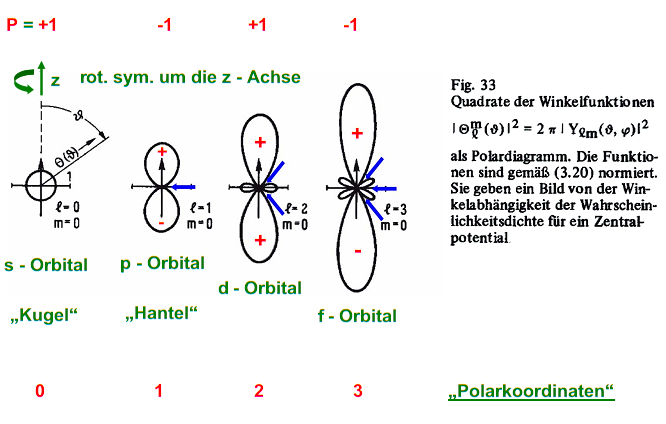
\includegraphics[width=\textwidth]{fig/3-KnotenPolarkoordinaten.png}
\end{figure}

Mit den Lösungen für $\Phi_m$ und $T_{lm}$ lassen sich die
$Y_{lm}$ angeben,
\begin{align*}
Y_{lm}(\th,\ph) = T_{lm}(\th)\Phi_m(\ph) = \frac{1}{\sqrt{2\pi}}
N_{lm}P_l^m(\cos\th)e^{im\ph}.
\end{align*}
Die Kugelflächenfunktionen $Y_{lm}$ sind die Eigenfunktionen zu $\op{l}^2$ und $\op{l}_z$,
\begin{align*}
&\op{l}^2Y_{lm} = \hbar (l+1)l Y_{lm}, && l=0,1,2,3,\ldots\\
&\op{l}_zY_{lm} = \hbar mY_{lm}, && \abs{m} \le l.
\end{align*}

Der Faktor $(l+1)$ kommt im Bohr'schen Atommodell nicht vor und folgt aus der
Wellennatur. Das bedeutet aber, dass der Drehimpulszustand nicht perfekt
gemessen werden kann, denn $\op{l}^2$ ist immer größer als $\op{l}_z^2$.
Selbst für maximales $m$, ($m=\pm l$) zeigt $\op{l}$ nicht exakt in
$z$-Richtung.

\begin{figure}[!htbp]
\centering
\begin{pspicture}(0,-1.67)(2.36,1.69)
\psline{->}(1.16,-1.65)(1.18,1.55)

\psellipse[linestyle=dashed,dashsep=0.06cm](1.18,-0.02)(1.18,0.33)
\psellipse[linestyle=dashed,dashsep=0.06cm](1.19,0.61)(0.97,0.26)
\psellipse[linestyle=dashed,dashsep=0.06cm](1.18,1.11)(0.68,0.2)
\psellipse[linestyle=dashed,dashsep=0.06cm](1.19,-0.65)(0.97,0.26)
\psellipse[linestyle=dashed,dashsep=0.06cm](1.18,-1.15)(0.68,0.2)

\psline[linecolor=darkblue]{->}(1.18,-0.03)(1.86,1.09)
\psline[linecolor=darkblue]{->}(1.18,-0.03)(2.16,0.59)
\psline[linecolor=darkblue]{->}(1.18,-0.03)(2.34,-0.03)
\psline[linecolor=darkblue]{->}(1.18,-0.01)(1.88,-1.17)
\psline[linecolor=darkblue]{->}(1.18,-0.01)(2.16,-0.67)

\rput[r](1.1,-0.025){\color{gdarkgray}\footnotesize$0$}
\rput[r](1.1,-1.165){\color{gdarkgray}\footnotesize$-2\hbar$}
\rput[r](1.1,-0.645){\color{gdarkgray}\footnotesize$-\hbar$}
\rput[r](1.1,0.595){\color{gdarkgray}\footnotesize$\hbar$}
\rput[r](1.1,1.095){\color{gdarkgray}\footnotesize$2\hbar$}
\rput(1.06,1.595){\color{gdarkgray}$z$}
\end{pspicture}
\caption{Mögliche Ausrichtung des Drehimpulses für $l=2$, $m=-2,-1,0,1,2$.}
\end{figure}

Für $m\neq 0$ haben die Kugelflächenfunktionen außerdem eine $(\sin\th)^m$
Abhängigkeit. Für $m\to\infty$ wird die Aufenthaltswahrscheinlichkeit jedoch in
die Äquatorialebene gedrückt, was wieder dem Korrespondenzprinzip entspricht.

Betrachtet man die räumliche Darstellung der Kugelflächenfunktionen, so sieht
man, dass die Quantenzahlen die Knotenflächen zählen. In den Knotenflächen ist
die Aufenthaltswahrscheinlichkeit Null.


\begin{figure}[H]
	\centering
	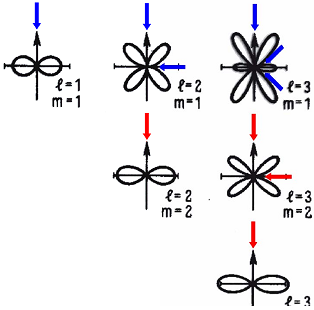
\includegraphics[width=0.5\textwidth]{fig/3-Kugelflaechenfunk.png}
	\caption{Knotenflächen der Kugelflächenfunktionen $\abs{Y_{lm}}^2$ in
	Abhängigkeit von $l$ und $m$.}
	%TODO: Mathematica
\end{figure}


\begin{figure}[!htbp]
	\centering
	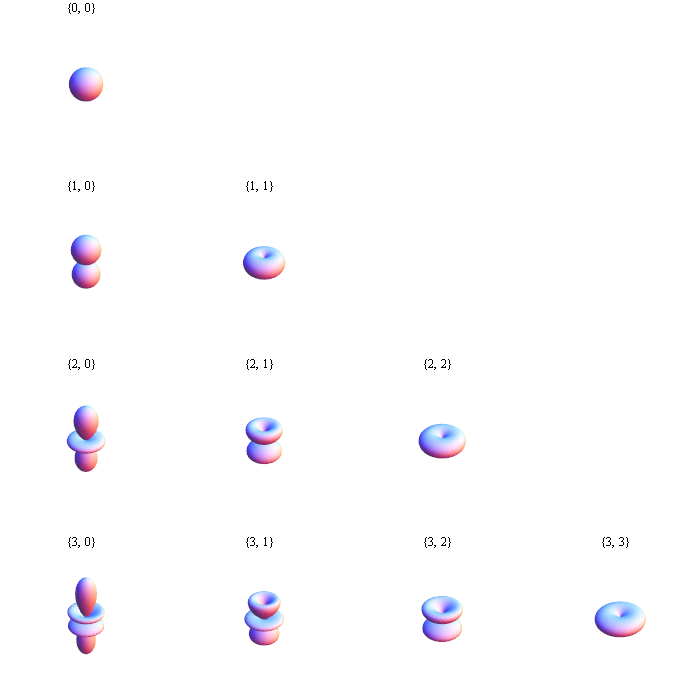
\includegraphics[width=0.8\textwidth]{fig/3-Kugelflaechenfunktionen.png}
	\caption{Graphische Darstellung zugeordneter Kugelflächenfunktionen.}
\end{figure}

%TODO: Bild Äquatorialdrehimpuls

%TODO: Bild Orbitale

\subsubsection{Radialgleichung}

Zur Lösung der Radialgleichung führen wir die Substitution $u = rR(r)$
durch.
\begin{align*}
\abs{u(r)}^2\dr = \abs{R(r)}^2r^2\dr
\end{align*}
beschreibt die Aufenthaltswahrscheinlichkeit des Elektrons in der Kugelschale
mit Radius $[r,r+\dr]$.

Die Gleichung nimmt nun eine uns bekannte Form an,
\begin{align*}
\frac{\diffd^2u}{\dr^2} + \frac{2m}{\hbar}\left[E-\underbrace{V(r) -
\frac{l(l+1)}{2mr^2}}_{V_{\text{Eff}}}\right]u = 0.
\end{align*}
Für die Energie erhalten wir so,
\begin{align*}
E_n = -\frac{R_\infty}{n^2},\qquad n=1,2,3,\ldots,\quad l\le n-1.
\end{align*}
Betrachtet man das effektive Potential, stellt man fest, dass für $l=0$ das
Elektron eine endliche Aufenthaltswahrscheinlichkeit im Kern hat. Es pendelt
quasi durch den Kern. Für $l>0$ wird die Potentialbarriere für abnehmendes $r$
immer größer, die Aufenthaltswahrscheinlichkeit im Kern ist Null.

\sfigure[H][0.8]%
	{3-EffektivesPotFuerRadial.pdf}
	{\KuckukAtom, S. 66}
	{Zum Zentrifugalpotential. a) Zustandekommen des effektiven Potentials, b,c)
	Wirkung der Potentialform auf die radiale Wellenfunktion $R(r)$.}
% 
% \begin{figure}[!htbp]
% 	\centering
% 	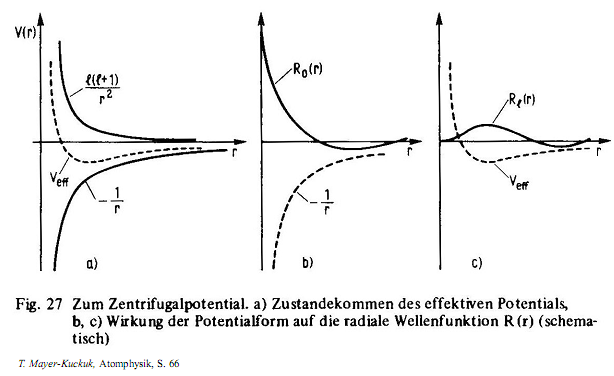
\includegraphics[width=\textwidth]{fig/3-EffektivesPotFuerRadial.png}
% \end{figure}

Betrachten wir Lösungen für $l=0$,
\begin{align*}
&R_{10}(\rho) =
2\left(\frac{Z}{a_0}\right)^{\frac{3}{2}} 1 \exp\left[-\frac{\rho}{2} \right],\\
&R_{20}(\rho) = \frac{1}{2\sqrt{2}}\left(\frac{Z}{a_0}\right)^{\frac{3}{2}}
(2-\rho) \exp\left[-\frac{\rho}{2} \right],\\
&R_{30}(\rho) = \frac{1}{9\sqrt{3}}\left(\frac{Z}{a_0}\right)^{\frac{3}{2}}
(6-6\rho-\rho^2) \exp\left[-\frac{\rho}{2} \right],
\end{align*}
mit $\rho = \frac{2Zr}{na_0}$, so werden diese durch die Laguerre-Polynome
beschrieben.

Erhöht man $l$ unter festem $n$, so verliert man bei jeder Erhöhung eine
Knotenfläche. Bei $l=n-1$ sind keine Knotenflächen mehr vorhanden.
$R_{nl}$ hat $(n-1)-l$ Nullstellen.

\sfigure[H][0.6]%
	{3-RadialteilWellenfunktion.pdf}
	{\HakenWolf, S. 171}
	{a) Die Wellenfunktion des Radialteils $R(r)$ des H-Atoms ist gegenüber der
	dimensionslosen Koordnate $\rho$ aufgetragen. Die an den Kurven angegebenen
	Indizes $(1,0)$, $(2,1)$, \ldots usw. entsprechen $(n,l)$, wobei $n$ die
	Hauptquantenzahl und $l$ die Drehimpulsquantenzahl. b) Die entsprechenden
	Aufenthaltswahrscheinlichkeiten in radialer Richtung. d.h. $4\pi \rho^2
	(\tilde{R}(\rho))^2$ sind gegenüber der dimensionslosen Koordinate $\rho$
	aufgetragen.}

\sfigure[H]%
	{3-EigenfunktionenDesWasserstoffatoms.pdf}
	{\KuckukAtom, S. 70}
	{Einige vollständige Eigenfunktionen des Wasserstoffatoms.}


\subsubsection{Anwendung der H-Atom Wellenfunktion}

Eine Schwäche des Bohr-Sommerfeld-Modells ist, dass man nicht vorhersagen
kann, wie wahrscheinlich ein Übergang zwischen zwei Energieniveaus ist und
daher die Lichtstärken im Spektrum des H-Atoms nicht erklären kann.

Wir wollen nun die Lösung der Schrödingergleichung für das H-Atom
interpretieren und dadurch einige Probleme des Bohr-Sommerfeld-Modells
lösen.

\begin{enumerate}[label=\arabic{*}.)]
\item Aufenthaltswahrscheinlichkeit des Elektrons im Kern.
\begin{align*}
l=0 \Rightarrow
\abs{\Psi_{n00}(r=0)}^2 = \abs{R_{n0}Y_{00}}^2 = \frac{Z^2}{\pi a_0^3n^3} \neq
0.
\end{align*}
D.h. wir haben eine endliche Aufenthaltswahrscheinlichkeit, die mit zunehmendem
$n$ abnimmt.
\begin{align*}
l>0\Rightarrow
\abs{\Psi_{nlm}(r=0)}^2 = \abs{R_{nl}Y_{lm}}^2 = 0,
\end{align*}
d.h. dass Elektronen mit $l>0$ keine Wechselwirkung mit einem punktförmigen Kern
haben.
\item Für den Erwartungswert des ``Bahnradius'' erhalten wir
\begin{align*}
\lin{r} = \int_{\R^3}\Psi^*r\Psi \dV = \frac{a_0}{2Z}\left((3n)^2 -l(l+1)
\right).
\end{align*}
$\lin{r}$ ist proportional zu $n^2$, was sich auch mit den Vorhersagen des
Bohr-Sommerfeld-Modell deckt. Für maximalen Drehimpuls $l=n-1$ und große
$n$ ist $l\approx n$ und daher
\begin{align*}
\lin{r} \sim \frac{a}{2Z}2n^2 = \frac{a}{Z}n^2,
\end{align*}
was gerade dem Radius der Kepplerbahn entspricht.

Für die Varianz erhalten wir,
\begin{align*}
&\lin{r^2}-\lin{r}^2 =
\begin{cases}
\frac{n^2(n^2+2)}{4Z^2} a_0^2, & \text{für }l=0,\\
\frac{n^2(2n+1)}{4Z^2} a_0^2, & \text{für }l=n-1,
\end{cases}\\
&\frac{(\Delta r)^2}{\lin{r}^2} =
\begin{cases}
\frac{1}{9}, & \text{für }l=0,\\
\frac{1}{2n}, & \text{für }l=n-1, 
\end{cases}
\end{align*}
d.h. die Unschärfe verschwindet für $n\to\infty$ und $l=n-1$, was gerade dem
Korrespondenzprinzip entspricht.

Für den Fall, dass alle Quantenzahlen groß werden,
\begin{align*}
n\to\infty,\quad l = n-1,\quad m=l,
\end{align*}
erhalten wir wieder die klassischen Kreisbahnen. Diese hoch angeregten Zustände
finden wir in \emph{zirkularen Rydbergatomen}.
\item Die Linienstärke im Spektrum ist proportional zur Wahrscheinlichkeit des
Dipolübergangs ($i$ - initial state, $f$ - final state)
\begin{align*}
\sim \abs{d_{i\to f}}^2 = \int_{\R^3} \Psi_f^* \op{d} \Psi_i \dV.
\end{align*}
Falls das Integral verschwindet, d.h. $\abs{d_{i\to f}}^2 = 0$ ist der Übergang
verboten und daher keine Linie im Spektrum sichtbar.

Wir wissen bereits, dass die Kugelflächenfunktionen den Winkelanteil der
Wellenfunktion des H-Atoms beschreiben und dass diese Eigenfunktionen des
Paritätsoperators sind. Wir können damit Auswahlregeln für optische
Übergange erarbeiten, denn damit $d_{if}\neq 0$ muss die Parität des
Integranden gerade sein, d.h. das Produkt von $\Psi_i$ und $\Psi_f$ muss
ungerade Parität haben. Die Partität der $Y_{lm}$ ist $(-1)^l$. Man kann
zeigen, dass nur Übergänge mit
\begin{align*}
&\Delta l = \pm 1
\end{align*}
erlaubt sind. Berücksichtigt man noch den Drehimpuls des Photons, das bei einem
optischen Übergang emittiert wird, erzwingt dies
\begin{align*}
\Delta m = 0,\pm 1.
\end{align*}
Das Bohr-Sommerfeld-Modell konnte dies nicht erklären. Die Übergänge wurden
lediglich postuliert (ohne physikalisches Verständnis). Jetzt können wir die
Übergänge erklären und quantifizieren. Ist $d_{i\to f}$ endlich, beginnt ein
Dipol bei der Übergangsfrequenz zu schwingen.
%TODO: l=0, l=1, usw. bildchen
Die Übergangsfrequenz ist viel höher als die Absorptions bzw. Emissionsrate, es
sind daher viele Oszillationen notwendig, bis der Übergang abgeschlossen ist.
Optische Übergänge entsprechen also Oszillationen hoher Güte. Die Dämpfung
durch die Abstrahlung ist dabei schwach. Die Anregungsenergie wird dabei in Form
von Photonen abgegeben.
\end{enumerate}

\newpage
\subsection{Drehimpuls und Spin}
\subsubsection{Klassische Betrachtung}
Klassisch betrachtet, bewegt sich das Elektron auf einer Kreisbahn um den Kern.
Damit ist ein Strom
\begin{align*}
I = \frac{a}{\tau} = -\frac{e}{T} = -\frac{ev}{2\pi r},
\end{align*}
verbunden, der die Fläche $A=\pi r^2$ umschließt.
\begin{figure}[!htbp]
\centering
\begin{pspicture}(0,-0.91411114)(1.94,0.91411114)

\psellipse[linestyle=dotted,dotsep=0.06cm](0.78,0.02)(0.78,0.32)
\psline{->}(1.42,0.2)(1.72,-0.02)
\psline[linecolor=darkblue]{->}(0.78,0.02)(0.78,0.9)
\psline[linecolor=purple]{->}(0.78,-0.32)(0.78,-0.9)
\psline{->}(0.78,0.02)(1.38,0.18)
\psbezier[linecolor=yellow]{->}(0.94,-0.29)(1.1,-0.28)(1.32,-0.22)(1.44,-0.14)
\psdots[linecolor=yellow](1.42,0.2)

\rput(0.63,-0.715){\color{gdarkgray}$\vec{l}$}
\rput(1.85,0.06){\color{gdarkgray}$\vec{v}$}
\rput(1.1,-0.05){\color{gdarkgray}$r$}
\rput(1.5,0.45){\color{gdarkgray}$e^-$}
\rput(1.24,-0.455){\color{gdarkgray}$I+$}
\rput(0.58,0.785){\color{gdarkgray}$\vec{\mu}$}
\end{pspicture} 
\qquad \qquad
\begin{pspicture}(0,-1.6)(3.2,1.6)
\psline{->}(1.1608791,0.37188306)(1.1608791,1.5175323)
\psellipse(1.1608791,0.37188306)(1.1608791,0.54554725)
\psline(1.1608791,-0.17366418)(1.1608791,-1.5375323)

\psline(1.1608791,0.37188306)(1.558022,-0.11910945)
\psline(1.1608791,0.37188306)(2.2912087,0.23549627)
\psline[linecolor=yellow]{->}(1.558022,-0.11910945)(2.2912087,0.23549627)
\psline[linecolor=darkblue]{<-}(1.558022,-0.11910945)(1.1608791,-1.3738681)
\psline[linecolor=purple]{->}(1.1608791,-1.3738681)(2.2912087,0.23549627)

\psbezier{<-}(1.894066,0.044554725)(2.54,-0.14246769)(1.7457143,-0.48099253)(2.48,-0.6424677)
\psbezier(1.1608791,-0.55554724)(1.24,-0.5224677)(1.34,-0.6224677)(1.36,-0.7424677)
\psbezier{<-}(1.2830769,-0.6646567)(0.6720879,-0.82832086)(1.1303297,-1.1010945)(0.64153844,-1.2374814)

\psbezier(1.36,0.13458785)(1.54,0.13458785)(1.66,0.23458785)(1.68,0.31458786)
\psline{->}(2.66,0.85458785)(2.66,1.5145879)
\psbezier{->}(0.94,0.19458786)(1.06,0.43458787)(1.14,0.034587856)(1.38,0.27458787)

\rput(2.83,1.0995878){\color{gdarkgray}\small$\vec{B}$}

\rput(0.9,1.45){\color{gdarkgray}\small$\omega_L$}

\rput(1.7,0.5025323){\color{gdarkgray}\tiny$\abs{\vec{l}}\sin\th$}

\rput(1,0.05){\color{gdarkgray}\tiny$\omega_L\Delta t$}

\rput(1.84,-0.6974677){\color{purple}\small$\vec{l}'$}

\rput(1.53,-0.4974677){\color{darkblue}\small$\vec{l}$}

\rput(2.68,-0.6374677){\color{gdarkgray}\small$\Delta \vec{l}$}

\rput(0.48,-1.2574677){\color{gdarkgray}\small$\th$}
\end{pspicture} 
\caption{Klassisches magnetisches Dipolmoment (links)
Präzession eines Kreisels miit Bahndrehimpuls $\vec{l}$ in einem auf das
Dipolmoment $\vec{\mu}$ wirkendem Feld $\vec{B}$ (rechts)}
\end{figure}
Durch diesen Strom wird ein magnetisches Dipolmoment induziert,
\begin{align*}
\mu = I \cdot A = -
\frac{ev}{2\pi r}\pi r^2.
\end{align*}
Mit $\vec{l} = m\left(\vec{r}\times\vec{v}\right)$ ist,
\begin{align*}
\vec{\mu} = -\underbrace{\frac{e}{2mc}}_{=:\mu_B}\vec{l}.
\end{align*}
Wobei $\mu_B$ als \emph{Bohr'sches Magneton} bezeichnet wird.

Befindet sich das Atom in einem äußeren Magnetfeld, wechselwirken das Feld und
der Dipol. Die Energie des Dipols im äußeren
Magnetfeld $\vec{B}$ ist
\begin{align*}
V_{\text{pot}} = -\vec{\mu}\vec{B}.
\end{align*}
Das daraus resultierende Drehmoment
\begin{align*}
\vec{M} = \vec{\mu}\times\vec{B} = \frac{\diffd\vec{l}}{\dt}
\end{align*}
bewirkt eine Änderung des Drehimpulses.
Nun ist
\begin{align*}
&\Delta \vec{l} = \omega_L \Delta t \abs{\vec{l}}\sin\th\\
\Rightarrow\; &
\frac{\diffd \vec{l}}{\dt} = \omega_L \abs{\vec{l}}\sin\th
\overset{!}{=} \abs{\vec{\mu}}\abs{\vec{B}}\sin\th\\
\Rightarrow\; & \omega_L = \frac{\mu B}{l} = -\frac{eB}{2mc}.
\end{align*}
Infolge des Drehmoments präzediert also $\vec{l}$ um $\vec{B}$ mit der
Winkelfrequenz $\omega_L$, der sogenannten \emph{Larmor-Frequenz}.

\subsubsection{Quantenmechanische Betrachtung}

In unserem bisherigen Modell hatten wir ein kugelsymmetrisches
Coulombpotential angenommen. Durch das induzierte Magnetfeld der
Elektronenbewegung wird jedoch eine Richtung ausgezeichnet und daher die
Kugelsymmetrie gebrochen. Wir wollen nun untersuchen, wie wir dies in unserer
Beschreibung mit Hilfe der Schrödingergleichung einbringen können.

Aufgrund der beobachteten Symmetrien und des Korrespondenzprinzips gilt auch in
der Quantenmechanik $\op{\mu}\parallel\op{l}$.
\begin{align*}
&\op{\mu} = c\cdot\op{l},\qquad c \in\R = \const.\\
\Rightarrow & \mu_z = \pm g_l \mu_M m_l,
\end{align*}
wobei $g_l$ den \emph{g-Faktor}, $m$ die Magnetquantenzahl und $\mu_M$ das
\emph{Einheitsmoment} bezeichnen. $g_l$ beschreibt, wie groß das
quantenmechanische Moment im Vergleich zum klassischen ist.
\begin{align*}
&\mu_M = \frac{q\hbar}{2mc}, && \text{Einheitsmoment},\\
&\mu_B = \frac{e\hbar}{2m_ec}, && \text{Elektron},\\
&\mu_K = \frac{e\hbar}{2m_pc}, && \text{Kern}.
\end{align*}
\begin{bspn}
Für das Elektron ist $\mu_B = \frac{e\hbar}{2m_ec} = 0.58\cdot
10^{-4}\frac{\mathrm{eV}}{\mathrm{T}}$.\bsphere
\end{bspn}
Da $\op{\mu}\parallel\op{l}$, erfüllen $\op{\mu}$ und $\op{l}$ dieselben
Vertauschungsrelationen, d.h. man kann bspw. nur $\op{\mu}_z$ und $\op{\mu}^2$
gleichzeitig messen und misst man $\op{\mu}_z$, so misst man automatisch
$\op{l}_z$ und vice versa.

Betrachten wir das Magnetfeld $\vec{B}=(0,0,B_z)$, so führt das magnetische
Moment zu einer Energieaufspaltung. Diese ist gegeben durch,
\begin{align*}
V = \op{\mu}_z \op{B}_z = g_l \mu_B m_l B_z,\qquad m_l = -l,\ldots,l, 
\end{align*}
d.h. es gibt $2l+1$ äquidistante Energieniveaus pro $l$-Zustand. Diese
Aufspaltung nennt man den \emph{Zeeman-Effekt}, der erstmals 1896 von Pieter Zeeman\footnote{Pieter
Zeeman (* 25. Mai 1865 in Zonnemaire Schouwen-Duiveland, Zeeland, Niederlande;
† 9. Oktober 1943 in Amsterdam) war ein niederländischer Physiker und
Nobelpreisträger für Physik des Jahres 1902.} beobachtet wurde.

\begin{figure}[!htbp]
\centering
\begin{pspicture}(0,-1.38)(4.38,1.8)

\psline[linecolor=purple](0.0,-1.36)(1.18,-1.36)
\psline[linecolor=purple,linestyle=dotted,dotsep=0.06cm](1.22,-1.36)(1.98,-1.36)
\psline[linecolor=purple](2.02,-1.36)(3.4,-1.36)

\psline[linecolor=darkblue](0.0,0.44)(1.18,0.44)
\psline[linecolor=darkblue,linestyle=dotted,dotsep=0.06cm](1.2,0.44)(2.0,1.04)
\psline[linecolor=darkblue,linestyle=dotted,dotsep=0.06cm](1.2,0.44)(1.98,0.44)
\psline[linecolor=darkblue,linestyle=dotted,dotsep=0.06cm](1.2,0.44)(2.0,-0.16)
\psline[linecolor=darkblue](2.0,1.04)(3.38,1.04)
\psline[linecolor=darkblue](2.0,0.44)(3.38,0.44)
\psline[linecolor=darkblue](2.0,-0.16)(3.38,-0.16)

\psline{<->}(3.36,0.98)(3.36,0.5)

\rput(3.88,0.745){\color{gdarkgray}$\mu_BB$}

\rput[r](3.65,1.205){\color{gdarkgray}$+1$}
\rput[r](3.65,0.385){\color{gdarkgray}$0$}
\rput[r](3.65,-0.235){\color{gdarkgray}$-1$}
\rput[r](3.65,1.5){\color{gdarkgray}$m$}

\rput(0.61,0.725){\color{gdarkgray}$p$}

\rput(0.59,-1.115){\color{gdarkgray}$s$}
\end{pspicture} 
\caption{Aufspaltung der $s$ und der $p$ Linie des H-Atoms im Magnetfeld.}
\end{figure}

Messungen der Larmorfrequenz zeigen $g_l=1$. Dies deckt sich auch mit
der klassischen Erwartung.

Neben dem Bahndrehimpuls gibt es jedoch noch eine weitere Quelle für das
magnetische Drehmoment, den Spin, der 1921 im Stern-Gerlach-Experiment entdeckt wurde.

Mit dem Bohr-Sommerfeld-Modell wurde zu diesem Zeitpunkt gerade vorhergesagt,
dass neben der Quantelung des Bahnradius und der Exzentrität auch die
Orientierung des magnetischen Moments im Raum gequantelt ist.
Stern\footnote{Otto Stern (* 17. Februar 1888 in Sohrau, Oberschlesien; † 17.
August 1969 in Berkeley) war ein deutscher, später in die USA emigrierter
Physiker.} und Gerlach\footnote{Walther Gerlach (* 1. August 1889 in Biebrich
am Rhein; † 10. August 1979 in München) war ein deutscher Physiker.} wollten
mit ihrem Experiment diese Quantisierung nachweisen.

\begin{figure}[!htbp]
	\centering
	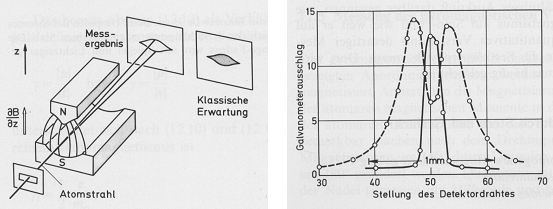
\includegraphics[width=\textwidth]{fig/3-SternGerlachExperiment.png}
	\caption{Aufbau des Stern-Gerlach Experiments}
\end{figure}

Im Experiment wurde ein Silberstrahl durch ein sehr inhomogenes Magnetfeld
auf eine Fotoplatte gestrahlt. Die neutralen Silberatome besitzen ein
magnetisches Moment, das sich am Feld ausrichtet. Klassisch müsste jede
Ausrichtung des magnetischen Moments möglich sein und daher ist eine
kontinuierliche Verteilung im Magnetfeld zu erwarten.

Die quantenmechanische Betrachtung besagt, dass die Atome abhängig von ihrem 
$\mu_z$-Zustand diskrete Winkel einstellen. Diejenigen mit $\mu_z = 0$ werden
das Magnetfeld gerade durchqueren, andere werden sich zu den Bereichen
mit dichteren bzw. dünneren Magnetfeldlininen verschieben. Geht man davon aus,
dass alle Atome sich im gleichen $l$-Zustand befinden, müssten nach unserer
bisherigen Überlegung auf der Platte $2l+1$, d.h. eine ungerade Zahl
3,5,7,\ldots an Linien zu sehen sein. Man sah jedoch genau 2. Ursache hierfür
ist der Spin der Elektronen im Silber $s=\frac{1}{2}\Rightarrow 2s+1 = 2$.

Zu diesem Zeitpunkt wusste man jedoch noch nichts über den Spin und dass die
Elektronen im Silber im Grundzustand Spin $\frac{1}{2}$ und Drehimpuls Null
haben. Für einen Nachweis der Aufspaltung reichte der Befund jedoch aus. 1927,
6 Jahre später, haben Phipps und Taylor die Aufspaltung in zwei Linien auch
beim Wasserstoff nachgewiesen.

% TODO: Weglassen oder Herr Pfau fragen 
% Im Silberatom tragen die Elektronen in den ``geschlossenen Schalen'' nichts
% zum Spin bei, da dieser sich gerade wegmittelt
% ($\uparrow\downarrow\uparrow\downarrow$). Dennoch stehen mehrere
% ``Valenzelektronen'' zur Verfügung. Die Frage ist nun, wie das magentische
% Moment aufgrund des Bahndrehimpulses und das aufgrund des Spins zu einem
% Gesamtdrehimpuls koppeln.

Das Experiment zeigt, dass es neben dem magnetischen Moment hervorgerufen durch
den Bahndrehimpuls $l$ auch eines aufgrund des Spins $s$ gibt,
\begin{align*}
\op{\mu}_s = g_s \mu_B \frac{\op{s}}{\hbar}.
\end{align*}
Der Elektronenspin ist auch makroskopisch messbar, was bereits 1915 im
Einstein-de-Haas-Experiment\footnote{Wander Johannes de Haas (* 2. März 1878 in
Lisse nahe Leiden; † 26. April 1960 in Bilthoven) war ein niederländischer
Physiker und Mathematiker.} durchgeführt wurde. Dabei beobachtet man einen
einen Eisenstab im homogenen Magnetfeld. Dieses führt dazu, dass sich die
Elektronenspins in eine Richtung ausrichten. Kehrt man nun das Magnetfeld um,
drehen sich auch die magnetischen Momente des Spins, was zu einem Drehmoment
führt. Dieses Drehmoment kann man messen und damit $g_s$ berechnen.
\begin{align*}
\Rightarrow g_s \approx 2.
\end{align*}
Der Spin erzeugt also ein dopplet so großes magnetisches Moment, wie eine
klassisch mit $\frac{1}{2}\hbar$ rotierende geladene Kugel.  Das magnetische
Moment aufgrund des Spins ``funktioniert'' also anders als das aufgrund des
klassischen Bahndrehimpulses. Es ist ein rein quantenmechanischer Effekt ohne
klassischen Grenzfall.

Um den $g$-Faktor des Spins zu erklären, müssen wir relativistische Effekte
berücksichtigen. Die Schrödingergleichung ist eine nichtrelativistische
Gleichung. Dirac\footnote{Paul Adrien Maurice Dirac, OM (* 8. August 1902 in
Bristol; † 20. Oktober 1984 in Tallahassee) war ein britischer Physiker,
Nobelpreisträger für Physik des Jahres 1933 und Mitbegründer der
Quantenphysik.} erweiterte die Schrödingergleichung auf die spezielle
Relativitätstheorie, indem er forderte, dass sie die relativistische
Energie-Impuls-Beziehung erfüllen muss und nur eine 1. Ableitung nach der Zeit
enthalten darf.

Er stellte fest, dass nur eine Wellenfunktion, die von mindestens 4 Parametern
abhängt, diese Forderungen erfüllen kann. Das erste Parameterpaar stellt dabei
das Teilchen mit Spin Up und Down dar und das zweite Parameterpaar das
Antiteilchen mit Spin Up und Down.

Dirac errechnete mit dieser Theorie, dass $g_s=2$ exakt. Der Nobelpreisträger
Dehmelt\footnote{Hans Georg Dehmelt (* 9. September 1922 in Görlitz) ist ein
deutsch-US-amerikanischer Physiker und Nobelpreisträger für Physik des Jahres
1989.} bestimmte jedoch 1987 die Größe experimentell mit sehr hoher Präzession auf,
\begin{align*}
g_s = 2.002319304386.
\end{align*}
Feynman\footnote{Richard Phillips Feynman (* 11. Mai 1918 in New
York; † 15. Februar 1988 in Los Angeles) war ein US-amerikanischer Physiker
und Nobelpreisträger für Physik des Jahres 1965.} erweiterte die Theorie von
Dirac durch die Korrekturterme,
\begin{align*}
g_s = 2.00 \left(1 + \frac{\alpha}{2\pi} + \ldots \right),\qquad \alpha \text{
Feinstrukturkonstante}
\end{align*}
und war damit in der Lage auch die Nachkommastellen korrekt vorherzusagen. Der
Unterschied zwischen theoretischem und empirisch ermittelten Wert beträgt
heute $\frac{\Delta g}{g} = 10^{-11}$.

Dies ist auch ein Anhaltspunkt dafür, wie ``gut'' die Quantenmechanik ist. Jede
Theorie, die die Quantenmechanik wiederlegen bzw. ersetzen will, müsste
mindestens die selbe Präzession erreichen.

\subsubsection{Addition von Drehimpulsen}

Wir wollen nun den Fall untersuchen, wenn sowohl Spin als auch
Bahndrehimpuls vorhanden sind. Klassisch addieren sich Bahndrehimpuls $\vec{l}$
und Spin $\vec{s}$ vektroriell zum Gesamtdrehimpuls $\vec{j}$,
\begin{align*}
\vec{j} = \vec{l} + \vec{s}.
\end{align*}

In der Quantenmechanik sind $\op{s}$ und $\op{l}$ unscharf, z.B. sind nur
Betrag und die $z$-Komponente bekannt und daher $x$- und $y$-Komponente
unscharf. Diese Unschärfe überträgt sich auch auf $\op{j}$.

\begin{figure}[!htbp]
\centering
\begin{pspicture}(0,-1.534)(3,1.534)
\psellipse(0.99,0.76)(0.99,0.41)
\psline(0.98,-1.25)(0.0,0.73)
\psline(2.16,0.09)(2.76,0.39)
\psline{->}(0.98,-1.53)(0.98,1.53)
\psline[linestyle=dotted,dotsep=0.06cm](1.96,0.73)(0.98,0.73)
\psline(0.98,-1.23)(1.34,0.49)

%\rput{-23.744934}(0.40731186,0.4171894){\psellipse(1.1958715,-0.76012886)(0.42806548,0.14858808)}
%\rput{-26.793932}(0.060014352,0.82076675){\psellipse(1.753021,0.28439686)(0.4606442,0.1815386)}

\rput{-23.744934}(-0.032369815,1.0057698){\psellipse(2.3758714,0.5798712)(0.42806548,0.14858808)}
\rput{-26.793932}(0.06001435,0.82076675){\psellipse(1.753021,0.28439686)(0.4606442,0.1815386)}

\psline[linecolor=darkblue]{->}(0.98,-1.25)(1.98,0.73)
\psline[linecolor=purple]{->}(0.98,-1.25)(2.18,0.09)
\psline[linecolor=yellow]{->}(2.16,0.09)(1.98,0.73)
%\psline[linecolor=yellow]{->}(0.98,-1.25)(0.8,-0.61)

\rput(2.05,-0.385){\color{purple}$\op{l}$}

\rput(2.27,0.3){\color{yellow}$\op{s}$}

\rput(2.14,1.1){\color{darkblue}$\op{j}$}

\rput(0.8,0.915){\color{gdarkgray}$\op{j}_z$}

%\rput(0.7,-0.985){\color{yellow}$\op{s}$}
\end{pspicture}
\begin{pspicture}(0,-1.5511667)(2.7977192,1.5511667)
\psellipse(0.99,-0.54705554)(0.99,0.41)
\psline(0.98,-1.26)(0,-0.58)
\psline(2.16,0.06119258)(2.725889,-0.20294444)
\psline{->}(0.9858889,-1.5370556)(0.9858889,1.5370556)
\psline[linestyle=dotted,dotsep=0.06cm](1.96,-0.59705555)(0.98,-0.59705555)
\psline(0.98,-1.2370555)(1.34,0.48294446)
\rput{24.358875}(0.042940438,-1.0163105){\psellipse(2.3758714,-0.4086787)(0.42806548,0.14858796)}
\rput{-26.793932}(0.06319487,0.82000923){\psellipse(1.753021,0.2773413)(0.4606442,0.1815386)}
\psline[linecolor=darkblue]{->}(0.98,-1.2570555)(1.9858888,-0.58294445)
\psline[linecolor=yellow]{->}(2.16,0.06119258)(1.98,-0.5788074)
\psline[linecolor=purple]{->}(0.98,-1.2570555)(2.18,0.082944445)

\rput(2.215889,-0.175){\color{yellow}$\op{s}$}
\rput(1.4458889,-1.1779444){\color{darkblue}$\op{j}$}
\rput(2.275889,0.23){\color{purple}$\op{l}$}
\rput(0.82,-0.51794446){\color{gdarkgray}$\op{j}_z$}
\end{pspicture} 

\caption{Addition von $\op{s}$ und $\op{l}$ zu $\op{j}$. Maximale Einstellung
(links) und minimale Einstellung (rechts).}
\end{figure}

Die Eigenwertgleichungen des Gesamtdrehimpulses $\op{j}$ ergeben sich analog
zu den des Drehimpulses $\op{l}$ und des Spins $\op{s}$,
\begin{align*}
&\op{l}^2\ket{l,m_l} = l(l+1)\hbar^2\ket{l,m_l},\\
&\op{s}^2\ket{s,m_s} = s(s+1)\hbar^2\ket{s,m_s},\\
\Rightarrow\;&\op{j}^2\ket{j,m_j} = j(j+1)\hbar^2\ket{j,m_j},\\
&\op{l}_z\ket{l,m_l} = m_l\hbar\ket{l,m_l},\\
&\op{s}_z\ket{s,m_s} = m_s\hbar\ket{s,m_s},\\
\Rightarrow\;&\op{j}_z\ket{j,m_j} = m_j\hbar\ket{j,m_j}.
\end{align*}
Über die Eigenwerte wissen wir,
\begin{align*}
&l\le n-1,\quad
m_l = -l,\ldots,l,\quad
m_s = -s,\ldots,s.
\end{align*}
Wie verhält es sich nun mit den Eigenwerten des Gesamtdrehimpulses?
\begin{align*}
&\op{j}_z = \op{l}_z + \op{s}_z,\qquad
\Rightarrow  m_j = m_l + m_s,
\end{align*}
Wir können also Maximal- und Minimalwerte von $m_j$ angeben und damit auch den
Wertebereich von $j$. Für $l>s$ gilt,
\begin{align*}
& m_j^{\small\text{max}} =
m_l^{\small\text{max}} + m_s^{\small\text{max}} = l+s = j^{\small\text{max}},\\
& m_j^{\small\text{min}} =
m_l^{\small\text{min}} + m_s^{\small\text{min}} = l-s = j^{\small\text{min}},\\
\Rightarrow & j = l-s,l-s+1,\ldots,l+s. 
\end{align*}
Für ein einzelnes Elektron ist $s=\frac{1}{2}$, d.h. es gibt zu gegebenem
$l$ jeweils nur zwei mögliche Gesamtdrehimpulse $j$ (außer für $l=0$). Für $m_j$
gibt es dafür $2j+1$ Einstellmöglichkeiten.
\begin{figure}
\centering
\begin{pspicture}(-0.1,-1.4)(3.6,1.8)
\psline{->}(1.06,-1.31)(1.06,1.31)
\psarc(1.06,-0.13){1.06}{270.0}{90.0}
\psline[linecolor=darkblue]{->}(1.06,-0.11)(1.84,0.5841111)
\psline[linecolor=darkblue]{->}(1.06,-0.09)(1.86,-0.8158889)
\psline[linecolor=darkblue]{->}(1.06,-0.11)(2.08,0.16411111)
\psline[linecolor=darkblue]{->}(1.06,-0.09588889)(2.1,-0.3358889)

\psline[linestyle=dotted,dotsep=0.06cm](1.06,0.15)(2.08,0.16411111)
\psline[linestyle=dotted,dotsep=0.06cm](1.06,-0.33)(2.1,-0.31588888)
\psline[linestyle=dotted,dotsep=0.06cm](1.06,0.59)(1.84,0.59)
\psline[linestyle=dotted,dotsep=0.06cm](1.86,-0.81)(1.06,-0.81)

\rput(0.83,1.4){\color{gdarkgray}$\op{j}_z$}
\rput(2.76,1.4){\color{gdarkgray}$m_j$}

\rput[r](3,0.6){\color{gdarkgray}$3/2$}
\rput[r](3,0.15){\color{gdarkgray}$1/2$}
\rput[r](3,-0.35){\color{gdarkgray}$-1/2$}
\rput[r](3,-0.8){\color{gdarkgray}$-3/2$}

\rput[r](0.9,0.6){\color{gdarkgray}$3/2\hbar$}
\rput[r](0.9,0.15){\color{gdarkgray}$1/2\hbar$}
\rput[r](0.9,-0.35){\color{gdarkgray}$-1/2\hbar$}
\rput[r](0.9,-0.8){\color{gdarkgray}$-3/2\hbar$}
\end{pspicture} 
\caption{Einstellmöglichkeiten für $\op{j}_z$ für $j=\frac{3}{2}\hbar$}
\end{figure}

\begin{bspn}
$l=2$, $s=\frac{1}{2}$, dann ist $j=\frac{3}{2}$ oder $\frac{5}{2}$.\bsphere
\end{bspn}

\begin{figure}[!htbp]
\begin{tabular}{r|c|c|c|c}
 & $s$ & $p$ & $d$ & $f$\\
$l$ & $0$ & $1$ & $2$ & $3$\\\hline
$j$ & $\frac{1}{2}$ & $\frac{1}{2}$, $\frac{3}{2}$ & $\frac{3}{2}$,
$\frac{5}{2}$ & $\frac{5}{2}$, $\frac{7}{2}$\\\hline
Notation & $S_{1/2}$ & $P_{3/2}$, $P_{3/2}$ & $D_{3/2}$, $D_{5/2}$ & $F_{5/2}$,
$F_{7/2}$
\end{tabular}
\caption{Mögliche Gesamtdrehimpulse für ein Einelektronen-Atom.}
\end{figure}

\newpage
\subsection{Atome im Magnetfeld - Zeeman Effekt}

Um zu verstehen, wie sich Atome im Magnetfeld verhalten, müssen wir untersuchen,
wie das magnetische Moment des Drehimpulses $\op{\mu}_l$ und das des
Spins $\op{\mu}_s$ zu einem Gesamtmoment $\op{\mu}_j$ koppeln.

Während $\op{\mu}_s\parallel \op{s}$ und $\op{\mu}_l\parallel \op{l}$, gilt
aufgrund der verschiedenen $g$-Faktoren für $s$ und $l$ nun
$\op{\mu}_j\nparallel \op{j}$.

Des Weiteren sind $\op{l}$ und $\op{s}$ durch die magnetische
Wechselwirkung aneinander gekoppelt. Dabei wechselwirken die 
magnetischen Momente (Dipol/Dipol-Wechselwirkung) und resultieren in konstanten
Energiewerten. Z.B. wird die Wechselwirkungsenergie im tiefsten Zustand
konstant minimal gehalten.

Unser Ziel ist es nun, $\op{\mu}_j$ durch Größen auszudrücken, die wir
gleichzeitig messen können, das sind
\begin{align*}
\op{j}_z, \op{j}^2, \op{l}^2, \op{s}^2.
\end{align*}

\subsubsection{Klassische Betrachtung}

Zeeman beobachtete (1896) eine Aufspaltung der Spektrallininen im Magnetfeld,
lange bevor man überhaupt ein Verständinis über das Zustandekommen der
Spektrallinien hatte.

Das klassische Modell geht zurück auf Lorentz. Wir betrachten ein Elektron auf
einer festen Kreisbahn mit Radius $r$, Zentrifugal- und Coulombkraft
kompensieren sich gerade.

Im Magnetfeld wirkt aufgrund der Bewegung eine zusätzliche Kraft, die
Lorentzkraft,
\begin{align*}
&F_L = \frac{1}{c}e\left(\vec{v}\times \vec{B}\right) = \frac{1}{c}e\omega' r
B,\\
\Rightarrow & m\omega^2 r = m\omega'^2r + \frac{1}{c} e \omega' rB,\\
\Leftrightarrow & \frac{m\left(\omega^2 - \omega'^2 \right)}{\omega'} =
\frac{1}{c}eB.
\end{align*}
Entwickle in $\omega$ mit $\Delta \omega = \omega - \omega'$
\begin{align*}
&\frac{\omega^2 - \omega'^2}{\omega'} = 
\frac{\left(\Delta\omega + \omega'\right)^2 - \omega'^2}{\omega'}
= \frac{\Delta \omega^2 + 2\omega'\Delta\omega + \omega'^2 -
\omega'^2}{\omega'}
\approx 2\Delta \omega\\
\Rightarrow &\Delta \omega = \pm \frac{eB}{2mc} = \pm
\omega_{\text{Larmor}}
\end{align*}
Je nach Umlaufsinn wird daher das Elektron schneller bzw. langsamer.

\begin{figure}[!htbp]
\centering
\begin{pspicture}(0,-1.41)(7.09,1.41)
\psline[linestyle=dotted,dotsep=0.06cm](1.4,-0.09)(1.4,1.11)
\psline[linecolor=darkblue](0.2,-0.09)(0.2,1.11)
\psline[linecolor=purple](2.58,-0.09)(2.58,1.11)
\psline{->}(0.0,-0.09)(3.02,-0.09)

\rput(0.25,1.255){\color{gdarkgray}$\sigma^-$}
\rput(2.65,1.255){\color{gdarkgray}$\sigma^+$}
\rput(2.85,-0.225){\color{gdarkgray}$\omega$}
\rput(1.9,-0.345){\color{gdarkgray}$\omega_L$}
\psline(1.4,-0.21)(1.4,-0.09)
\psline(2.58,-0.09)(2.58,-0.21)

\rput(1.41,-0.785){\color{gdarkgray}2 Linien}

\psline[linecolor=yellow](5.46,-0.09)(5.46,1.11)
\psline[linecolor=darkblue](4.26,-0.09)(4.26,1.11)
\psline[linecolor=purple](6.64,-0.09)(6.64,1.11)
\psline{->}(4.06,-0.09)(7.08,-0.09)

\psline{<->}(6.4,0.91)(6.9,0.91)
\psline{<->}(5.38,0.43)(5.38,1.01)
\psline{<->}(4.02,0.91)(4.52,0.91)

\rput(4.31,1.255){\color{gdarkgray}$\sigma^-$}
\rput(6.71,1.255){\color{gdarkgray}$\sigma^+$}
\rput(6.91,-0.225){\color{gdarkgray}$\omega$}
\rput(5.5,-0.305){\color{gdarkgray}$\omega_0$}
\rput(5.47,1.275){\color{gdarkgray}$\pi$}

\rput(5.47,-0.785){\color{gdarkgray}3 Linien}

\rput(1.4,-1.185){\color{gdarkgray}z-Richtung}
\rput(5.48,-1.185){\color{gdarkgray}x,y-Ebene}
\end{pspicture} 
\caption{Spektrum des Zeeman-Effekts (schematisch).}
\end{figure}

Klassisch ist das Elektron als ``rotierende Antenne'' zu verstehen.
In $z$-Richtung beobachtet man links- und rechts zirkular polarisiertes Licht,
sogenanntes $\sigma^-$ bzw. $\sigma^+$-Licht.
In der $x,y$-Ebene beobachtet man neben dem in $z$-Richtung zirkular
polarisiertem $\sigma^-$ und $\sigma^+$ Licht, auch noch
linear polarisierts $\pi$-Licht.
Dies nennt man den \emph{normalen Zeeman-Effekt}.

\sfigure[H][0.6]%
	{3-AufspaltungNormalerZeemanEffekt.pdf}
	{\HertelSchulz, S. 287}
	{Aufspaltung bei normalen Zeeman-Effekt.}

\subsubsection{Quantenmechanische Betrachtung}

Das Elektron hat einen Bahndrehimpuls $\op{l}$ und einen Spin $\op{s}$,
der Gesamtdrehimpuls ist $\op{j}$. Wie verhält es sich nun mit dem
gesamtmagnetischen Moment?
\begin{align*}
\op{\mu}_j = \op{\mu}_s + \op{\mu}_l
= g_s \mu_B \frac{\op{s}}{\hbar} + g_l \mu_B \frac{\op{l}}{\hbar}
= \frac{\mu_B}{\hbar} \left(2\op{s} + \op{l}\right)
= \frac{\mu_B}{\hbar} \left(\op{j} + \op{s}\right)
 \nparallel \op{j}.
\end{align*}

\begin{figure}[!htbp]
\centering
\begin{pspicture}(0,-2.152)(2.38,2.18)
\psline[linecolor=darkblue]{->}(0.98,-0.2)(1.98,1.78)
\psline[linecolor=purple]{->}(0.98,-0.2)(2.18,1.14)
\psline[linecolor=yellow]{->}(2.16,1.14)(1.98,1.78)

\psline[linecolor=purple]{->}(0.98,-0.2)(0.42,-0.86)
\psline[linecolor=yellow]{->}(0.42,-0.86)(0.6,-1.5)
\psline[linecolor=darkblue]{->}(0.98,-0.2)(0.6,-1.46)

\psline[linestyle=dotted,dotsep=0.06cm]{<-}(0.02,-2.14)(1.02,-0.16)

\rput(2.05,0.665){\color{gdarkgray}$\vec{l}$}

\rput(2.27,1.505){\color{gdarkgray}$\vec{s}$}

\rput(1.6,1.65){\color{darkblue}$\vec{j}$}

\rput(0.47,-0.355){\color{gdarkgray}$\vec{\mu}_l$}

\rput(0.19,-1.135){\color{gdarkgray}$\vec{\mu}_s$}

\rput(1.08,-0.915){\color{darkblue}$\vec{\mu}_j$}
\end{pspicture}
\caption{Addition von $\vec{\mu}_s$ und $\vec{\mu}_l$ im Vergleich zu $\vec{s}$
und $\vec{l}$.}
\end{figure}

Wir wollen nun die Wechselwirkungsenergie des gesamtmagnetischen Moments mit
einem äußeren Magnetfeld berechnen. Dabei gehen wir zunächst davon aus, dass
dieses Feld ``schwach'' ist und die Orientierung von $\mu_s$ und $\mu_l$ nicht
verändert wird.
\begin{align*}
V_B = -\op{\mu}_j \op{B}.
\end{align*}
Um in einer ``guten Basis'' zu rechnen, projezieren wir $\op{\mu}$ auf
$\op{j}$ und $\vec{B}$ auf $\op{j}$,
\begin{align*}
V_B
=
\left(-\op{\mu}_j\frac{\op{j}}{\abs{\op{j}}}\right)\left(\frac{\op{j}}{\abs{\op{j}}}\op{B}\right)
=
\frac{\mu_B}{\hbar}\frac{\left(\op{s}+\op{j}\right)\op{j}\left(\op{j}\op{B}\right)}{\op{j}^2}
= \frac{\mu_B}{\hbar} B \op{j}_z \left(\frac{\op{j}^2 +
\op{s}\op{j}}{\op{j}^2}\right).
\end{align*} 
Wir wollen diesen Ausdruck nun auf Größen reduzieren, die wir gleichzeitig
messen können. Betrachte dazu,
\begin{align*}
\op{l}^2 = \left(\op{s}+\op{j}\right)^2 = \op{j}^2 + 2\op{s}\op{j} +
\op{s}^2.
\end{align*}
Einsetzen ergibt,
\begin{align*}
V_B = \frac{\mu_B}{\hbar} B \op{j}_z \left(\frac{\op{j}^2 - \frac{\op{j}^2 -
\op{l}^2 + \op{s}^2}{2}}{\op{j}^2} \right)
\end{align*}
Wir haben damit $V_B$ durch gleichzeitig messbare Größen ausgedrückt. Ersetzen
der Operatoren durch Eigenwerte, ergibt sich
\begin{align*}
\Delta E = \mu_B B m_j \underbrace{\left[ \frac{j(j+1) + \frac{1}{2}\left(j(j+1)
+ s(s+1) - l(l+1) \right)}{j(j+1)}\right]}_{:= g_j}.
\end{align*}
$g_j$ nennt man den \emph{Landé'schen
$g$-Faktor}, $g_j\in[1,2]$.
Die Energieaufspaltung aufgrund des Zeeman-Effekts findet also in
$2j+1$ äquidistante Niveaus statt.

\begin{bemn}[Bemerkungen.]
\begin{enumerate}[label=\arabic{*}.)]
  \item $s=0\Rightarrow j=l, g_j = 1 = g_l$,\\
$l=0\Rightarrow j=s, g_j = 2 = g_s$.
\item 
Übergänge zwischen den Niveaus können nur für $\Delta m_j = 0,\pm 1$
stattfinden. 
\item
Der \emph{normale Zeeman-Effekt} tritt auf, wenn der $g$-Faktor im angeregten
und im Grundzustand gleich ist. D.h. $s=0$, denn ein Übergang erfordert
$\Delta l = \pm 1$, dies ist nur bei
Mehrelektronen-Atomen möglich. Die Energieniveaus spalten sich dabei in eine
ungerade Anzahl $2l+1$ auf.

Der \emph{annomale Zeeman-Effekt} tritt in allen anderen Fällen auf. Die
Anzahl der Energieniveaus $2j+1$ kann hier auch gerade sein, wenn $j$
halbzahlig ist

Der normale Zeeman Effekt tritt also nur auf, wenn der Spin keine Rolle
spielt. Der annomale Zeeman-Effekt ist somit häufiger anzutreffen.\maphere
\end{enumerate}
\end{bemn}
 
\begin{bemn}[Ausblick.]
Im Abschnitt über Kernphysik haben wir gesehen, dass auch Protonen und
Neutronen einen Spin besitzen. Dieser kann ebenfalls mit den magnetischen
Momenten der Elektronen wechselwirken.

\begin{table}[h]
\begin{tabular}{l|c|l}
& \text{Spin} & \text{Landé-Faktor}\\\hline
Proton & $ \frac{1}{2}$ & $g_p = 5.586\ldots$\\
Neutron & $\frac{1}{2}$ & $g_n = -3.826\ldots$
\end{tabular}
\end{table}

Diese Wechselwirkung werden wir im Rahmen der Hyperfeinstruktur genauer
untersuchen.\maphere
\end{bemn}

\subsection{Feinstruktur}

Im Experiment sehen wir für gleiches $l$ aber unterschiedliches $j$ eine
weitere Aufspaltung der Energieniveaus. Sie heißt
\emph{Feinstrukturaufspaltung} und fasst mehrere Phänomenen zusammen. Um diese
zu erklären, müssen wir unser Modell weiter verfeinern. Dazu werden wir
zunächst die Kopplung des Spins $s$ und des Bahndrehimpulses $l$ untersuchen.
Anschließend werden wir - wie bereits im Bohr-Sommerfeld-Modell -
relativistische Korrekturen einführen, denn magnetische Phänomene sind
relativistische Wechselwirkungen 1. Ordnung.

\subsubsection{Spin-Bahn-Wechselwirkung}

Die Wechselwirkung des magnetischen Moments des Spins mit dem Magnetfeld
aufgrund der Bahnbewegung des Elektrons ruft eine Aufspaltung der Energieniveaus
hervor
\begin{align*}
\Delta E_{ls} = -\vec{\mu}_s\cdot \vec{B}_l,
\end{align*} 
wobei $\vec{\mu}_s$ das magnetische Moment des Spins im Ruhesystem des
Elektrons und $\vec{B}_l$ das Magnetfeld aufgrund des Bahndrehimpules $\vec{l}$
am Ort des Elektrons beschreibt.

\begin{figure}[!htbp]
\centering
\begin{pspicture}(0,-0.91411114)(1.94,0.91411114)

\psellipse[linestyle=dotted,dotsep=0.06cm](0.78,0.02)(0.78,0.32)
\psline{->}(1.42,0.2)(1.72,-0.02)
\psline[linecolor=darkblue]{->}(0.78,0.02)(0.78,0.9)
\psline{->}(0.78,0.02)(1.38,0.18)
\psdots[linecolor=yellow](1.42,0.2)

\rput(1.85,0.06){\color{gdarkgray}$\vec{v}$}
\rput(1.1,-0.05){\color{gdarkgray}$r$}
\rput(1.5,0.45){\color{gdarkgray}$e^-$}
\rput(0.58,0.785){\color{gdarkgray}$\vec{B}$}
\end{pspicture} 
 
\caption{Bewegung des Elektrons.}
\end{figure}

Das Ruhesystem des Elektrons ist jedoch ein beschleunigtes Bezugssystem
(Kreisbewegung), d.h. \textit{kein} Inertialsytem. Berechnen wir zunächst das
Magnetfeld mit dem Biot-Savart'schen Gesetz in diesem Bezugssystem,
\begin{align*}
\vec{B}_l = \frac{I}{c} \int\limits_0^{2\pi} \frac{\dvecs \times \vec{r}}{r^3}
= -\frac{eZ}{c}\frac{\vec{v}\times \vec{r}}{r^3}
= \frac{eZ}{mcr^3}\vec{l},
\end{align*}
müssen wir das Ergebnis ins Laborsystem zurücktransformieren. Die etwas
längliche Rechnung sei als Übungsaufgabe überlassen. Es ergibt sich,
\begin{align*}
\vec{B}_l = \frac{1}{2}\frac{Ze}{mcr^3}\vec{l}.
\end{align*}
Der Faktor $\frac{1}{2}$ heißt Thomas-Faktor und entsteht bei Transformation
von Nichtinertialsystemen. Übertragen wir dieses Ergebnis auf Operatoren
mit $\op{\mu}_s = -2\mu_B \frac{\op{s}}{\hbar}$ für $g_s = 2$
erhalten wir,
\begin{align*}
\Delta E_{ls} = -\op{\mu}_s \op{B}_l = 2\frac{e\hbar}{2mc}\frac{Ze}{2mcr^3}
\frac{\op{l}\op{s}}{\hbar} = \underbrace{\frac{Ze^2}{2m^2
c^2r^3}}_{\rho(r)}\op{l}\op{s}.
\end{align*}
Diesen Ausdruck kann man als Dipol/Dipol-Wechselwirkung identifizieren. Mit dem
Erwartungswert des H-Atoms von $\frac{1}{r^3}$ kann $\Delta E_{ls}$ berechnet
werden,
\begin{align*}
\Delta E_{ls} \approx 10^{-4}\mathrm{eV} \entspr 24.2 \mathrm{GHz}\quad
\Rightarrow\quad \frac{\Delta E_{ls}}{E}\approx 10^{-5}\mathrm{eV}.
\end{align*}
Der Wert ist klein im Vergleich zur Bindungsenergie aber relativ groß im
Frequenzspektrum, daher ist er auch schon so früh entdeckt worden.

Die Größe des Magnetfeldes das vom Bahndrehimpuls erzeugt wird,
\begin{align*}
B_l = \frac{\Delta E_{ls}}{\mu_B} =
\frac{10^{-4}\mathrm{eV}}{\mu_B} \approx 1T.
\end{align*}
Die Forderung, dass das äußere Magnetfeld ``schwach'' sein soll, bezieht sich
auf diese Größe. Erst wenn äußere Magnetfelder der Größenordnung 
$1\mathrm{T}$ anliegen, wird die Kopplung von $s$ und $l$ beeinflusst.

Betrachten wir nun die Änderung des Hamilton-Operators,
\begin{align*}
\op{H}_{\text{FS}} = \rho(r)\; \op{l}\op{s},
\end{align*}
und verwenden $\op{l}\op{s} = \frac{1}{2}\left(\op{j}^2 - \op{l}^2 -
\op{s}^2\right)$, ergibt sich
\begin{align*}
\lin{\Delta E_{ls}} = \lin{\op{H}_{\text{FS}}} = \lin{\rho(r)\op{l}\op{s}} = 
\lin{\rho(r)}\frac{\hbar^2}{2}\left[ j(j+1) - l(l+1)-s(s+1) \right],
\end{align*}
wobei $\lin{\rho(r)} = \frac{a}{\hbar^2}$. $a$ heißt
\emph{Spin-Bahn-Kopplungskonstante}. Für das H-Atom ist
\begin{align*}
\lin{\Delta E_{ls}} = a\cdot
\begin{cases}
\frac{l}{2},& \text{für }j=l+\frac{1}{2},\\
-\frac{l+1}{2},& \text{für }j=l-\frac{1}{2}.
\end{cases}
\end{align*}
\begin{figure}
\centering
\begin{pspicture}(0,-1.8)(9,1.8)
\psline(0.0,0.24)(1.0,0.24)
\psline[linecolor=darkblue,linestyle=dotted,dotsep=0.06cm](1.02,0.24)(1.82,0.84)
\psline[linecolor=purple,linestyle=dotted,dotsep=0.06cm](1.02,0.24)(1.82,-1.36)
\psline[linecolor=darkblue](1.82,0.86)(3.42,0.86)
\psline[linecolor=purple](1.82,-1.36)(3.42,-1.36)
\psline[linestyle=dotted,dotsep=0.06cm](1.06,0.24)(3.42,0.24)
\psline{<->}(2.0,0.78)(2.0,0.32)
\psline{<->}(2.0,0.16)(2.0,-1.28)

\rput(2.38,0.565){\color{gdarkgray}$a/2$}
\rput(2.28,-0.515){\color{gdarkgray}$-a$}
\rput(3.02,1.085){\color{gdarkgray}$2P_{3/2}$}
\rput(3.02,-1.575){\color{gdarkgray}$2P_{1/2}$}
\rput(4.33,1.625){\color{gdarkgray}Entartung}
\rput(4.3,1.085){\color{gdarkgray}4x}
\rput(4.3,-1.575){\color{gdarkgray}2x}
\rput[l](5,1.085){\color{gdarkgray}$m_j=-3/2,-1/2,1/2,3/2$}
\rput[l](5,-1.575){\color{gdarkgray}$m_j=-1/2,1/2$}
\end{pspicture}
\caption{Aufspaltung durch
Spin-Bahn-Wechselwirkung.}
\end{figure}

Die Lorentzkraft wirkt $\bot$ zur Bewegungsrichtung und verrichtet daher keine
Arbeit. Es kann somit nicht zur Verschiebung der Energie kommen. Wir sehen
dies auch bei der Aufspaltung, denn ${}^2 P_{3/2}$ ist 4-fach entartet, während
${}^2P_{1/2}$ lediglich 2-fach entartet ist. Der Linienschwerpunkt bleibt daher
erhalten. Für $l=0$ haben wir keine Aufspaltung.

Betrachten wir die Größe $a$ genauer,
\begin{align*}
a&:= \hbar^2 \lin{\rho(r)} = \hbar^2 \int R_{nl}^* \rho(r) R_{nl} r^2\dr
\ldots\\ &= \frac{mc^2}{2}(Z\alpha)^4 \frac{1}{n^3(l(l+\frac{1}{2})(l+1))},
\end{align*}
so ergibt sich als Energieskala die Ruheenergie $\frac{mc^2}{2}$.

Wenn wir die Spin-Bahn-Wechselwirkung in $\alpha$ entwickeln, hat diese die
Ordnung $\alpha^4$. Um die Wirkung vollständig zu beschreiben, müssen wir daher nach
anderen Effekten suchen, die die selbe Ordnung haben.

\subsubsection{Relativistische Massenzunahme}

Betrachte den relativistischen Ausdruck für die Energie des Elektrons,
\begin{align*}
E = c\sqrt{\vec{p}^2 + m^2 c^2}.
\end{align*}
und entwickle in $\vec{p}$, so ergibt sich
\begin{align*}
E = mc^2 + \frac{\vec{p}^2}{2m} - \frac{\vec{p}^4}{8m^3 c^2} + \ldots.
\end{align*}
Verglichen mit der Energie $\frac{\vec{p}^2}{2m}$ gilt für den ersten
relativistischen Korrekturterm
\begin{align*}
\frac{\vec{p}^4/8m^3 c^2}{\vec{p}^2/2m} = 4m^2\frac{\vec{p}^2}{c^2}
\sim
\left(\frac{v}{c}\right)^2 \approx \alpha^2 \sim 5\cdot 10^{-5}.
\end{align*}
Die Korrektur der relativistischen Massenzunahme hat daher die Ordnung
$\alpha^4$ und somit dieselbe Ordnung in $\alpha$ wie die
Spin-Bahn-Wechselwirkung. Sie erzeugt daher vergleichbar starke Effekte.

Für eine exakte Rechnung müssten wir nun zur relativistischen
Schrödingergleichung (Dirac) übergehen. Wir wollen uns jedoch mit Korrekturen
bis zur 4. Ordnung begnügen. Wenden wir die Störungstheorie auf die
H-Wellenfunktion an, ergibt sich,
\begin{align*}
\lin{\Delta E_{\text{rel}}} &= -\frac{\hbar^2}{8m^3c^4}\int_{\R^3} \Psi_{nlm}^*
\nabla^4 \Psi_{nlm} \dV \\
 &=
-\frac{mc^2}{2}\left(Z\alpha\right)^4\left(\frac{1}{n^3\left(l
+ \frac{1}{2}\right)} - \frac{3}{4n^4}\right).
\end{align*}

\subsubsection{Feinstrukturaufspaltung.}

Wir wollen nun die Abweichung aufgrund der Spin-Bahn-Wechselwirkung und der
relativistische Massenzunahme in der Feinstrukturaufspaltung zusammenfassen,
\begin{align*}
\Delta E_{\text{FS}} = \Delta E_{ls} + \Delta E_{\text{rel}}.
\end{align*}
Für das H-Atom mit $j=l\pm\frac{1}{2}$ ergibt sich somit,
\begin{align*}
\lin{\Delta E_\text{FS}} = -\frac{1}{2}mc^2\left(Z\alpha\right)^4
\frac{1}{n^3}\left( \frac{1}{j+\frac{1}{2}} - \frac{3}{4n},
\right).
\end{align*}
$\Delta E_{\text{FS}}$ ist also unabhängig von $l$, d.h. Zustände mit gleichem
$j$ aber unterschiedlichem $l$ und $s$ sind weiter entartet.

\begin{figure}[!htbp]
\centering
\begin{pspicture}(-0.4,-1.62)(8.36,1.62)
\psline[linecolor=darkblue](0.0,0.64)(0.82,0.64)
\psline[linecolor=purple,linestyle=dotted,dotsep=0.06cm](0.82,0.64)(1.82,1.24)
\psline[linecolor=darkblue,linestyle=dotted,dotsep=0.06cm](0.82,0.64)(1.82,-0.36)
\psline[linecolor=darkblue,linestyle=dotted,dotsep=0.06cm](0.82,0.64)(1.82,0.64)
\psline[linecolor=darkblue](1.8,0.64)(3.2193213,0.64)
\psline[linecolor=purple](1.8,1.24)(3.2193213,1.24)
\psline[linecolor=darkblue](1.82,-0.36)(3.2393212,-0.36)

\rput(0.42,0.805){\color{gdarkgray}$n=2$}

\rput(0.4,0.425){\color{gdarkgray}$l=0,1$}

\rput(2.8,1.42){\color{gdarkgray}$2P_{3/2}$}

\rput(2.8,0.82){\color{gdarkgray}$2S_{1/2}$}

\rput(2.8,-0.18){\color{gdarkgray}$2P_{1/2}$}

\psline[linecolor=purple,linestyle=dotted,dotsep=0.06cm](3.22,1.24)(4.24,0.84)
\psline[linecolor=darkblue,linestyle=dotted,dotsep=0.06cm](4.22,-0.56)(3.22,0.64)
\psline[linecolor=darkblue,linestyle=dotted,dotsep=0.06cm](3.22,-0.36)(4.22,-0.56)
\psline[linecolor=darkblue](4.22,-0.56)(6.42,-0.56)
\psline[linecolor=purple](4.24,0.84)(6.42,0.84)

\rput(6.0,1.02){\color{gdarkgray}$2P_{3/2}$}

\rput(5.53,-0.38){\color{gdarkgray}$2S_{1/2}$, $2P_{1/2}$}

\rput(2.49,-1.055){\color{gdarkgray}Spin-Bahn WW}

\rput(5.27,-1.055){\color{gdarkgray}Spin-Bahn WW}

\rput(6.24,-1.455){\color{gdarkgray}+ relativistische Korrekturen}
\end{pspicture}
\caption{Energieabsenkung aufgrund Spin-Bahn Wechselwirkung und
relativistischen Korrekturen.}
\end{figure}

Experimentell lassen sich die entarteten Zustände dennoch unterscheiden. Mit der
heutigen Präzessionsfrequenzmessung kann man weit über diese Korrekturen hinaus
messen. Unsere Korrektur bringt eine 5-Stellen Genauigkeit $\sim 10^{-5}$.
Heute kann man über $10^{-15}$ genau messen. Man müsste also mindestens Terme
bis zur Ordnung 8 aufnehmen, um die heutigen Messungen zu bestätigen.
Dabei ist zu berücksichtigen, dass es neben der Feinstruktur auch
eine Hyperfeinstruktur gibt. Diese beschreibt die Kopplung des magnetischen
Moments des Elektrons mit dem des Kerns. Da die Wechselwirkung
$\sim\frac{1}{m}$ ist, ist die des Kerns ca. 2000-mal kleiner als die Elektrons
und hat daher die Ordnung $\approx \alpha^5$. Liegt aber immernoch deutlich
über dem heute messbaren Bereich.


\subsection{Hyperfeinstruktur}


Bisher sind wir vom kugelsymmetrischen Coulomb-Potential ausgegangen
und haben die stationären Lösungen der Schrödingergleichung in diesem
Potential berechnet. Anschließend haben wir die Feinstrukturaufspaltung
berücksichtigt, die im Wesentlichen auf der magnetischen Wechselwirkung des
Elektronenspins mit dem Magnetfeld, welches durch die Bahnbewegung des
Elektrons erzeugt wird, beruht.

Bei Messungen mit sehr hoher Auflösung stellt man nun fest, dass die
Feinstrukturlinien im H-Atom selbst wieder aufgespalten sind. Diese Aufspaltung
ist (oft) kleiner als die Dopplerbreite, d.h. sie kann nur mit
\textit{dopplerfreien} spektroskopischen Methoden aufgelöst werden und heißt \emph{Hyperfeinstruktur}
der Spektrallinien.

Um diese zu erklären, betrachten wir den Kern des H-Atoms, das Proton, welches
als Spin $\frac{1}{2}$ Teilchen selbst ein magnetisches Moment trägt
\begin{align*}
\op{\mu}_p = g_p \mu_K \frac{\op{s}_p}{\hbar},
\end{align*}
wobei $\op{s}_p$ den Kernspin bezeichnet.\footnote{In der Literatur findet man
auch häufig die Bezeichnung $\op{i}$.} Das Kernmagneton ist
\begin{align*}
\mu_p = \frac{e\hbar}{2 c}\frac{1}{m_p} = \frac{m_e}{m_p} \mu_B \simeq
\frac{1}{1836}\mu_B.
\end{align*}
Der $g$-Faktor des Protons ist,
\begin{align*}
g_p = 5.59 \Rightarrow \frac{\mu_e}{\mu_p} = \frac{2}{5.59}\cdot 1836 \approx
658.
\end{align*}
Obwohl der $g$-Faktor des Protons größer ist, als der des Elektrons ist das
magnetische Moment des Protons wesentlich kleiner.
Die $\op{l}$, $\op{s}$ Kopplung bleibt daher auch unter Berücksichtigung des
Kernmoments dominant und wir können die Kernwechselwirkung im
Rahmen der Störungstheorie einführen. Diese Störung führt zu einer weiteren
Aufspaltung der Energieniveaus, sie heißt \emph{Hyperfeinstruktur}.

Die Energieaufspaltung erfüllt folgende
Proportionalität,
\begin{align*}
\Delta E_{\text{HFS}} \sim \frac{\op{\mu}_p\op{\mu}_l}{r^3},
\end{align*}
was wir als magnetische Dipol/Dipol-Wechselwirkung identifizieren können.
\begin{bspn}
Wasserstoff Atom. $\Delta E_{\text{HFS}} \approx 5\cdot 10^{-6}\mathrm{eV}<<
\Delta E_{\text{FS}} \approx 10^{-4}\mathrm{eV}$.\bsphere
\end{bspn}
$\op{s}_p$ und $\op{j}$ koppeln zu einem neuen totalen Drehimpuls $\op{f}$,
analog zur $\op{l}$, $\op{s}$-Kopplung,
\begin{align*}
\op{f} = \op{s}_p + \op{j}.
\end{align*}
$\op{f}^2$ hat die Eigenwerte $f(f+1)\hbar^2$, $\op{f}_z$ die Eigenwerte $m_f
\hbar$. Analog zu $\op{j}$ sehen wir, dass $f$ ganz und halbzahlig sein
kann,
\begin{align*}
&f = j+s_p,j+s_p-1,\ldots, \abs{j-s_p},\\
&m_f = -f,-f+1,\ldots,f
\end{align*}
Gleichzeitig beobachtbar sind $\op{l}^2$, $\op{s}^2$, $\op{j}^2$, $\op{s}_p^2$,
$\op{f}^2$ und $\op{f}_z$.

Drücken wir die Wechselwirkungsenergie durch die
Eigenwerte aus,
\begin{align*}
\lin{E_\text{HFS}} = A \frac{\lin{\op{s}_p\op{j}}}{\hbar} = \frac{A}{2}
\left[f(f+1)-j(j+1)-s_p(s_p+1)\right],
\end{align*}
wobei $A=\frac{g_p \mu_K}{\sqrt{j(j+1)}}B_0$ als \emph{Intervallfaktor}
bezeichnet wird mit $B_0$ dem effektiven Magnetfeld am Kernort.

Die Stärke des Magnetfelds $B_0$ am Kernort erfüllt die Proportionalität,
\begin{align*}
B_z \sim \frac{Z^3}{n^3}\sqrt{s(s+1)}.
\end{align*}
\begin{bspn}
Wasserstoff im Grundzustand. $s=\frac{1}{2}$, $l=0$, $j=\frac{1}{2}$, $s_p =
\frac{1}{2}$.
\begin{align*}
\Rightarrow\; &\Delta E_\text{HFS} = 
\begin{cases}
\frac{A}{4}, & \text{für } f=1,\quad \uparrow j \uparrow s_p,\\
-\frac{3A}{4}, & \text{für } f = 0,\quad \uparrow j\downarrow s_p.\\
\end{cases}
\end{align*}
Das Magnetfeld $B_0$ hat die Größenordnung,
\begin{align*}
&n=1 \Rightarrow B_0 \approx 29\mathrm{T},\\
&n=2 \Rightarrow B_0 \approx 3.6\mathrm{T}.
\end{align*}
Dies entspricht dem $B_l$ aus der $l$,$s$-Kopplung bis auf den Thomas
Faktor.

\begin{figure}[!htbp]
\centering
\begin{pspicture}(0,-1.79)(5.08,1.79)
\psline(0.0,0.23)(1.0,0.23)
\psline[linecolor=purple,linestyle=dotted,dotsep=0.06cm](1.02,0.23)(1.82,0.83)
\psline[linecolor=darkblue,linestyle=dotted,dotsep=0.06cm](1.02,0.23)(1.82,-1.37)
\psline[linecolor=purple](1.82,0.85)(3.42,0.85)
\psline[linecolor=darkblue](1.82,-1.37)(3.42,-1.37)
\psline[linestyle=dotted,dotsep=0.06cm](1.06,0.23)(3.42,0.23)
\psline{<->}(2.0,0.77)(2.0,0.31)
\psline{<->}(2.0,0.15)(2.0,-1.29)

\rput(4.33,1.615){\color{gdarkgray}Entartung}
\rput(4.3,0.995){\color{gdarkgray}3x}
\rput(4.28,-1.625){\color{gdarkgray}1x}
\rput(2.455889,0.515){\color{gdarkgray}$A/4$}
\rput(2.525889,-0.585){\color{gdarkgray}$3A/4$}
\rput(3.1,1.1){\color{gdarkgray}$f=1$}
\rput(3.1,-1.6){\color{gdarkgray}$f=0$}
\rput(0.5458889,0.455){\color{gdarkgray}$j=1/2$}
\rput(0.52588886,0.035){\color{gdarkgray}$l=0$}
\end{pspicture}
\caption{Hyperfeinstrukturaufspaltung im Wasserstoff.}
\end{figure}

Das Wasserstoffatom ist ein Boson, obwohl es aus Fermionen (Proton,
Elektron) besteht. Deren halbzahlige Spins ($s=\frac{1}{2}$, $s_p=\frac{1}{2}$)
addieren sich zu einem ganzzahligen ($0,1$). Bei starkem Abkühlen geht ein
spinpolarisiertes Gas ununterscheidbarer H-Atome in ein
Bose-Einstein-Kondensat über.

Für Deuterium ist $s_p = 1$ und daher der Gesamtspin halbzahlig.
Als Fermion verhält es sich bei starkem Abkühlen wie ein Fermigas.\bsphere
\end{bspn}
Die Hyperfeinstruktur beruht auf der magnetischen Wechselwirkung, welche keine
Arbeit verrichtet, denn $\vec{F}\sim \vec{v}\times\vec{B}\Rightarrow
\vec{F}\bot \vec{v}$. 
Wie bei der Feinstrukturaufspaltung bleibt daher der Linienschwerpunkt erhalten.

Für beliebiges $F$, d.h. auch in ``komplexen'' Kernen gilt die Formel,
\begin{align*}
\Delta E_\text{F+1} - \Delta E_{F} =
\frac{A}{2}\left[F(F+1) - (F+1)(F+2)\right] = A[F+1].
\end{align*}
Sie heißt \emph{Invervallregel}.
\begin{figure}[!htbp]
\centering
\begin{pspicture}(-0.2,-1.8)(6.72,1.8)
\psline(-0.1,-0.24)(1.0,-0.24)
\psline[linecolor=darkblue,linestyle=dotted,dotsep=0.06cm](1.02,-0.24)(1.7858889,0.92)
\psline[linestyle=dotted,dotsep=0.06cm](1.06,-0.24)(3.42,-0.24)

\rput(5.97,1.625){\color{gdarkgray}Entartung}

\rput(0.5,-0.035){\color{gdarkgray}$J=5/2$}
\rput(0.5,-0.455){\color{gdarkgray}$I=3/2$}

\psline[linecolor=darkblue,linestyle=dotted,dotsep=0.06cm](1.0058889,-0.24)(1.7858889,-0.48)
\psline[linecolor=darkblue,linestyle=dotted,dotsep=0.06cm](1.0058889,-0.24)(1.7858889,-1.28)
\psline[linecolor=darkblue,linestyle=dotted,dotsep=0.06cm](1.0058889,-0.24)(1.7858889,-1.68)
\psline[linecolor=darkblue](1.7858889,0.92)(3.42,0.92)
\psline[linecolor=darkblue](1.7858889,-0.48)(3.42,-0.48)
\psline[linecolor=darkblue](1.7858889,-1.28)(3.42,-1.28)
\psline[linecolor=darkblue](1.7858889,-1.68)(3.42,-1.68)

\rput(3.025889,0.325){\color{gdarkgray}$4A$}
\rput(3.045889,-0.895){\color{gdarkgray}$3A$}
\rput(3.025889,-1.495){\color{gdarkgray}$2A$}
\rput(4.26,1.625){\color{gdarkgray}$F$}
\rput(6.02,1.305){\color{gdarkgray}$2F+1$}

\rput(4.17,0.925){\color{gdarkgray}$4$}
\rput(4.17,-0.435){\color{gdarkgray}$3$}
\rput(4.17,-1.215){\color{gdarkgray}$2$}
\rput(4.17,-1.635){\color{gdarkgray}$1$}

\rput[c](6.05,0.945){\color{gdarkgray}$9$}
\rput[c](6.05,-0.435){\color{gdarkgray}$7$}
\rput[c](6.05,-1.215){\color{gdarkgray}$5$}
\rput[c](6.05,-1.635){\color{gdarkgray}$3$}

\rput(2.1,-0.355){\color{gdarkgray}\tiny$-1/4$}
\end{pspicture} 
\caption{Zur Intervallregel.}
\end{figure}

Die HFS-Übergänge sind als magnetische Dipol/Dipol-Übergänge zwar sehr
schwach, da jedoch sehr viel Wasserstoff im Universum existiert, lässt sich
auch sehr viel dieser Strahlung messen. Die Strahlung, die bei
Hyperfeinstruktur-Übergängen entsteht, durchdringt aufgrund der niedrigen
Frequenz auch optisch dichte Bereiche im Universum. Ihre Messung und
Interpretation liefert daher Bilder von sonst unzugänglichen Bereichen.

\begin{bemn}[Bemerkungen.]
\begin{enumerate}[label=\arabic{*}.)]
  \item Die Übergänge in der HFS-Aufspaltung des H-Atoms im Grundzustand
  emittieren Strahlung der Frequenz $1420\mathrm{MHz}$. Diese Strahlung
   ist die Grundlage für die Radioastronomie. In den 50ern wurde diese
 Strahlung erstmals gemessen. Heute wird der ganze Himmel mit immer besser werdenden Teleskopen überwacht. Die gemessene Intensität gibt Aufschluss
darüber, wie viel Wasserstoff im Universum existiert. Die Messung der
Frequenzverschiebung (Dopplereffekt) und die Berücksichtigung relativistischer
Effekte gibt uns Informationen darüber, wie schnell sich der Wasserstoff bewegt.
\item $1420\mathrm{MHz}\entspr 70\mathrm{mK}$. Die Hintergrundtemperatur liegt
bei $2.7\mathrm{K}$, d.h. $F=1$ ist bereits thermisch angeregt.

Man hat festgestellt, dass manchen den Bereichen, in denen die Wasserstoff
Konzentration hoch ist, auch mehr Wasserstoff mit $F=1$ als mit $F=0$
existiert (Maseraktivität). Diese Populationsinversion kann z.B. durch
inhomogene Magnetfelder dynamisch erzeugt werden.
\item Die Sekunde ist über die Hyperfeinstrukturaufspaltung im Cäsiumatom
($s=\frac{1}{2}$, $s_p=\frac{7}{2}$) definiert. Im Cäsium entspricht der
Übergang zwischen $F=3$ und $F=4$ gerade
$9.2\mathrm{MHz}$.

Da die Frequenzmessung in Cäsium-Uhren sehr genau möglich ist
\begin{align*}
\frac{\delta\nu}{\nu} \approx 10^{-15},
\end{align*}
 wurde diese Frequenz verwendet, um die
Sekunde zu definieren.\maphere
\end{enumerate}
\end{bemn}


\subsection{Paschen-Back-Effekt vs. Zeeman-Effekt}

Bisher sind wir davon ausgegangen, dass das äußere Magnetfeld ``klein'' ist.
Zeeman-Effekt, Feinstruktur und Hyperfeinstruktur haben zu folgenden
Korrekturen im Hamiltonian geführt,
\begin{align*}
\op{H} = \ldots \op{p}^2 + \underbrace{\ldots
\op{l}\op{s}}_{\text{Spin-Bahn-Kopplung}} + \underbrace{\ldots
\op{p}^4}_{\text{rel. Korrekturen}} +
\underbrace{\ldots\op{\mu}\op{B}}_{\text{Zeeman}} + \underbrace{\ldots
\op{j}\op{s}_p}_{\text{Kopplung Kern, $e^-$}}.
\end{align*}
Die Korrekturen sind nur so lange gültig, wie $\op{\mu}_s \op{B}_\text{ext}$
klein gegenüber der Kopplung von $\op{l}$ und $\op{s}$ bzw.
$\op{\mu}_{p}\op{B}_\text{ext}$ klein gegenüber der Kopplung von $\op{j}$ und
$\op{s}_p$ ist. Wir wollen nun die Größenordnung abschätzen, ab der wir
$\op{\mu}\op{B}_\text{ext}$ nicht mehr als kleine Störung betrachten können.
Diesen Fall bezeichnet man als \emph{Paschen-Back-Effekt}.

Das magnetische Moment des Kerns ist gegeben durch,
\begin{align*}
\op{\mu}_p = g_p \mu_B \frac{\op{s}_p}{\hbar},\quad g_p \approx 5.58,
\quad
\frac{\mu_K}{\mu_B} = \frac{1}{1836}.
\end{align*}
Die Energieaufspaltung durch die Hyperfeinstruktur ist gegeben durch,
\begin{align*}
\Delta E_{\text{HFS}} = \frac{A}{2}\left( f(f+1)-j(j+1)-s_p(s_p+1)
\right),\quad A = \frac{g_p \mu_K}{\sqrt{j(j+1)}}B_0.
\end{align*}
\begin{bspn}
Effektives Magnetfeld der Elektronenhülle am Kernort im Wasserstoff,
\begin{align*}
&n=1 \Rightarrow B_{0} \approx 29 \mathrm{T} &&\entspr
\Delta E_{\text{HFS}} = 5.9\cdot 10^{-6} \mathrm{eV},\\
&n=2 \Rightarrow B_{0} \approx 3.6 \mathrm{T} &&\entspr \Delta E_{\text{HFS}} =
7.3 \cdot 10^{-7}\mathrm{eV}.
\end{align*}
Man kann Magnetfelder dieser Größe im Labor erzeugen, der Paschen-Back-Effekt
ist also beobachtbar.
Die Energieaufspaltung durch die Feinstruktur beträgt,
\begin{align*}
\Delta E_\text{FS} = 10^{-4}\mathrm{eV}.
\bsphere
\end{align*}
\end{bspn}
D.h. es gibt zwei Bereiche für starke Magnetfelder,
\begin{enumerate}[label=(\alph{*})]
  \item %$\op{\mu}_B > \frac{a}{\hbar^2} \op{l}\op{s}$.
  $B_\text{ext}> B_0$. Das äußere Magnetfeld ist stärker als das Magnetfeld der
  Elektronenhülle, so dass sowohl die Kopplung von $\op{l}$ und $\op{s}$
  also auch die von $\op{j}$ und $\op{s}_p$ aufgebrochen
  wird. Dieser Effekt heißt \emph{Paschen-Back-Effekt}.
  \item $B_\text{ext} > B_p$. Das äußere Magnetfeld ist lediglich stärker als
  das Magnetfeld des Kerns, so dass nur die Kopplung von $\op{j}$
  und $\op{s}_p$ aufgebrochen wird. Dieser Effekt heißt
  \emph{Paschen-Back-Effekt der Hyperfeinstruktur}.
\end{enumerate}

\subsubsection{Paschen-Back-Effekt}

Die Kopplung von $\op{l}$ und $\op{s}$ erfordert eine feste Phase zwischen
den Größen. In Abwesenheit bzw. Anwesenheit eines  schwachen
äußeren Magnetfelds, wird die feste Phase durch die Spin-Bahn-Kopplung erzeugt.
$\op{l}$ und $\op{s}$ sind einzeln unscharf, lassen sich aber aufgrund der festen Phase wohldefiniert zu $\op{j}$ addieren.

\begin{figure}[!htbp]
\centering
\begin{pspicture}(-0.1,-1.515)(1.8,1.7)
\psellipse[dotsep=0.06cm](0.86,0.76)(0.86,0.33)
\psellipse[dotsep=0.06cm](0.86,-0.05)(0.66,0.24)

\psline(0.01,0.71)(0.86,-1.11)
\psline[linecolor=darkblue]{->}(0.86,-1.11)(1.72,0.71)
\psline[linecolor=yellow]{<-}(0.2,-0.09)(0.86,-1.11)
\psline(0.86,-1.11)(1.51,-0.09)

\psline{->}(0.86,-1.51)(0.86,1.39)
\psline(0.8,0.77)(0.92,0.77)
\psline(0.8,-0.07)(0.92,-0.07)

\rput(0.4,1.5){\color{gdarkgray}$z$, $B_\text{ext}$}
\rput(0.65,0.815){\color{gdarkgray}$\op{l}_z$}
\rput(0.67,-0.025){\color{gdarkgray}$\op{s}_z$}
\rput(1.63,0.25){\color{gdarkgray}$\op{l}$}
\rput(0.39,-0.65){\color{gdarkgray}$\op{s}$}
\end{pspicture}
\caption{Aufhebung der $\op{l}$, $\op{s}$-Kopplung.}
\end{figure}

Falls $B_\text{ext} > B_0 \sim \frac{a}{\hbar^2}$ koppeln sowohl
$\op{l}$ als auch $\op{s}$ an das äußere Feld. $\op{s}$ und $\op{l}$
sind dann unabhängig voneinander, d.h. zwischen $\op{l}$ und $\op{s}$ besteht
keine feste Phase mehr. Auch $\op{s}_p$ entkoppelt. Die Summe $\op{l}+\op{s}$
wird unscharf und $j$, $m_j$ sind keine guten Quantenzahlen mehr.  Da aber die Kopplung von
$\op{l}$ und $\op{s}$ aufgehoben ist, sind nun $\op{l}^2$, $\op{l}_z$, $\op{s}^2$, $\op{s}_z$
gleichzeitig messbar. Die Energieaufspaltung ist gegeben durch,
\begin{align*}
\Delta E_\text{PB} = -\op{\mu} \op{B}_\text{ext} =
\frac{\mu_B}{\hbar}\left(\op{l}_z + 2\op{s}_z\right)\op{B}_\text{ext} = \mu_B
B_\text{ext} \left(m_l + 2m_s\right).
\end{align*}

\subsubsection{Paschen-Back-Effekt der Hyperfeinstruktur}

Ohne äußeres Magnetfeld koppeln $\op{s}_p$ und $\op{j}$ zu $\op{f}$ über die
Wechselwirkung zwischen $\op{\mu}_{s_p}$ und $B_j$. Gleichzeit messbar sind,
\begin{align*}
\op{j}^2, \op{l}^2, \op{s}^2, \op{s}_p^2, \op{f}^2, \op{f}_z.
\end{align*}
Für kleine äußere Magnetfelder bleibt diese Kopplung erhalten.

Ist nun $\vec{B}_\text{ext} > \frac{A}{\mu_K}$ aber $B_\text{ext} <
\frac{a}{\mu_B}$, so entkoppeln $\op{s}_p$ und $\op{j}$ aber die $\op{l}$,
$\op{s}$-Kopplung ist weiterhin dominant.
Die stärkste Wechselwirkung ist nun die magnetische Wechselwirkung von
$\op{\mu}_j$ mit dem äußeren Feld $\vec{B}_\text{ext}$. Analog zum
Zeeman-Effekt bilden sich $2j+1$-Niveaus aus mit
\begin{align*}
\Delta E_Z = \op{\mu}_j \op{B}_\text{ext} = g_j \mu_B m_j B_\text{ext}.
\end{align*}
Der nächst kleinere Term ist die Wechselwirkung des Kernmoments
$\op{\mu}_{p}$ mit dem Magnetfeld der Hülle $\vec{B}_0$,
\begin{align*}
\Delta E = \op{\mu}_{p} \op{B}_0 =  A m_j m_{s_p}
% g_p \mu_K \frac{\op{s}_{p_z}}{\hbar}
%\vec{B}_0 \overset{!}{=}
%g_p \mu_K \frac{\op{s}_{p_z}}{\hbar}
%\vec{B}_0 \frac{\op{j}}{j}=
%\frac{\mu_p B_K}{\hbar s_p j} \op{s}_p\op{j} B_0.
\end{align*}
Die Energieaufspaltung ist nun gegeben durch,
\begin{align*}
\Delta E_{\text{PB}}^\text{HFS} = g_j \mu_B m_j B_\text{ext} + A m_j m_{s_p} -
g_{s_p} \mu_K m_{s_p} B_\text{ext},
\end{align*}
wobei der letzte Term die Wechselwirkung des Kerns mit dem äußeren
Magnetfeld beschreibt und nur bei extrem hohen Feldern berücksichigt werden
muss.
%TODO: Aufspaltungsskizze
%3-HyperfeinaufspaltungPBderHFS.pdf
Man beobachtet also die Zeemanlinien der Hülle mit zusätzlicher
Hyperfeinstrukturaufspaltung.

\begin{bemn}[Bemerkungen.]
\begin{enumerate}[label=\arabic{*}.)]
  \item Der Übergang zwischen dem Zeeman und Paschen-Back Bereich ist nicht scharf
sondern kontinuierlich.
  \item Neben den bisher eingeführten Korrekturen gibt es noch den 
  \emph{Lamb-Shift}, der die Energieverschiebung aufgrund von 
  Vakuumfluktuationen beschreibt. Dieser wird in der Quantenfeldtheorie und
 der fortgeschrittenen Atomphysik ausführlicher behandelt.\maphere
\end{enumerate}
\end{bemn}

\sfigure%
	{3-HyperfeinaufspaltungPBderHFS.pdf}
	{\HertelSchulz, S. 366}
	{Hyperfeinaufspaltung im schwachen und Starken Magnetfeld.}

\sfigure[H]%
	{3-Drehimpulskopplung.pdf}
	{}
	{Übersicht zur Drehimpulskopplung.}

\subsection{He-Atom}


Bislang hatten wir unsere Betrachtung auf das H-Atom beschränkt, das sich als
Einelektronensystem in einem anziehenden Coulomb-Potential beschreiben ließ.
In diesem Fall ließ sich die Schrödungergleichung aufgrund der Kugelsymmetrie
des Coulomb-Potential in Radial- und Winkelanteil separieren und daher leicht
analytisch lösen.
Für Alkaliatome lässt sich dieses Modell aufrechterhalten indem man die vollen
Schalen und den Kern als effektives Einelektronensystem in einem abgeschirmten
anziehenden Coulomb-Potential zusammenfasst.
Für die übrigen Atome stößt dieses Modell jedoch auf Probleme, da sich die
Valenzelektronen ja paarweise gegenseitig abstoßen und dem Pauli-Prinzip
gehorchen müssen. 
Wir wollen die grundlegenden Probleme nun am Beispiel des Heliumatoms
diskutieren.

Das Helium-Atom hat die Kernladungszahl $Z=2$, es besteht aus $2$ Protonen im
Kern und $2$ Elektronen in der Hülle. Im Prinzip haben wir es hier mit einem
3-Köper-Problem zu tun, dem Kern und den zwei Elektronen.
\begin{figure}[!htpb]
\centering
\begin{pspicture}(-0.1,-0.8)(2.1,0.79)

\pscircle(1.0,-0.55){0.2}
\pscircle(0.14,0.39){0.14}
\pscircle(1.86,0.39){0.14}

\psline[linecolor=yellow]{<->}(0.32,0.41)(1.68,0.41)
\psline[linecolor=darkblue]{<->}(1.18,-0.39)(1.76,0.25)
\psline[linecolor=darkblue]{<->}(0.22,0.25)(0.86,-0.39)

\rput(1.01,-0.55){\color{gdarkgray}\small++}
\rput(1.86,0.37){\color{gdarkgray}\small-}
\rput(0.14,0.37){\color{gdarkgray}\small-}
\rput(1.04,0.595){\color{gdarkgray}$\vec{r}_{12}$}
\rput(1.67,-0.125){\color{gdarkgray}$\vec{r}_1$}
\rput(0.37,-0.125){\color{gdarkgray}$\vec{r}_2$}
\end{pspicture} 
\caption{Zum Dreikörperproblem.}
\end{figure}

 Das Potential dieses Systems ist gegeben durch,
\begin{align*}
V(\vec{r}_1,\vec{r}_2) = -\frac{Ze^2}{r_1} - \frac{Ze^2}{r_2} +
\frac{e^2}{r_{1,2}}.
\end{align*} 
Dabei ist ist der dritte Term, der die Wechselwirkung der Elektronen
untereinander beschreibt, der problematische, denn ohne diesen könnten wir uns
auf den Fall von zwei voneinander unabhängigen Zweikörperproblemen
zurückziehen. Die zeitunabhängige Schrödingergleichung hat nun die Form,
\begin{align*}
\left[\frac{\op{p}_1^2}{2m} + \frac{\op{p}_2^2}{2m} + V(r_1,r_2)
\right]\Psi(r_1,r_2) = E\Psi(r_1,r_2).
\end{align*}
Diese Schrödingergleichung ist nicht mehr exakt lösbar. Da auch das klassische
3 Körperproblem nicht allgemein analytisch lösbar ist, darf man das von der
Schrödingergleichung auch nicht erwarten. Es liegt keine Kugelsymmetrie vor, wir
sind daher nicht in der Lage die Gleichung in Radial- und Winkelanteil zu separieren. Es ist auch nicht möglich die Gleichung in zwei Einteilchen-Wellenfuktionen aufzuspalten, d.h.
\begin{align*}
\Psi(r_1,r_2) \overset{!}{\neq} \Psi(r_1)\Psi(r_2)!
\end{align*}

\subsubsection{Naiver Ansatz}

Um störungstheoretisch an das Problem heranzugehen, 
wollen wir zunächst den naiven Ansatz wählen, dass die Wechselwirkung der
Elektronen untereinander, $\frac{e^2}{r_{1,2}}$, klein ist, d.h.
\begin{align*}
V(\vec{r}_1,\vec{r}_2) = -\frac{Ze^2}{r_1} - \frac{Ze^2}{r_2}.
\end{align*} 
somit erhalten wir  zwei unabhängige ``H-artige'' Probleme, die wir durch
Separation lösen können,
\begin{align*}
\Psi(r_1,r_2) = \Psi(r_1)\Psi(r_2).
\end{align*}
Für die Energie erhalten wir die Gleichung,
\begin{align*}
E = -\left(\frac{RhcZ^2}{n^2}\right)_1 - \left(\frac{RhcZ^2}{n^2}\right)_2,
\end{align*}
was als Ionisierungsenergie $E_{\text{ion}} = -108.8\mathrm{eV}$ liefert. Im
Experiment sehen wir jedoch,
\begin{align*}
E_{\text{ion}} = -79\mathrm{eV},
\end{align*}
wobei
\begin{align*}
&E_{\text{ion},1} = -24.6\mathrm{eV},&& \text{Ionisierungenergie 1. Elektron},\\
&E_{\text{ion},2} = -54.4\mathrm{eV},&& \text{Ionisierungenergie 2. Elektron}.
\end{align*}
Dabei entspricht die Ionisierungsenergie des 2. Elektrons gerade dem vierfachen
von $13.6\mathrm{eV}$, was gut mit der Erwartung übereinstimmt, denn $Z=2$ und
$E\sim Z^2$. D.h. für Einelektronenatome wie $\mathrm{He}^+$ liefert der Ansatz
brauchbare Ergebnisse, für Mehrelektronenatome ist die Abweichung zu groß.

\subsubsection{Qualitative Aussagen}

Was können wir qualitativ über die Wellenfunktion des He-Atoms aussagen?
Nehmen wir die Spin-Bahn-Wechselwirkung als klein an, können wir die
Wellenfunktion in einen Spin und einen Ortsanteil separieren,
\begin{align*}
\Psi(\vec{r}_1,\vec{r}_2) =
\underbrace{\Phi(\vec{r}_1,\vec{r}_2)}_{\text{Ort}}\underbrace{\chi(\vec{r}_1,\vec{r}_2)}_{\text{Spin}}.
\end{align*}
Da das Elektron ein Fermion ist, muss die Wellenfunktion antisymmetrisch sein,
d.h. entweder ist die Spin-Wellenfunktion antisymmetrisch und die
Ortswellenfunktion symmetrisch oder umgekehrt,
\begin{align*}
\Psi_{1,2} = \Phi_s \chi_A\text{ oder } \Psi_{1,2} = \Phi_A \chi_S.
\end{align*}
Die allgemeine Form einer asymmetrischen Zweiteilchen-Wellfunktion ist,
\begin{align*}
\ket{\Psi}_{12} = \frac{1}{\sqrt{2}} \left( \ket{\alpha}_1\ket{\beta}_2 -
\ket{\beta}_1\ket{\alpha}_2\right).
\end{align*}
Eine Vertauschung von $\alpha$ und $\beta$ ändert offensichtlich das
Vorzeichen. Die allgemeine Form einer symmetrischen
Zweiteilchen-Wellenfunktion ist,
\begin{align*}
\ket{\Psi}_{12} = \frac{1}{\sqrt{2}} \left( \ket{\alpha}_1\ket{\beta}_2+
\ket{\beta}_1\ket{\alpha}_2\right).
\end{align*}
Vertauschung von $\alpha$ und $\beta$ ändert das Vorzeichen nicht.

Wir wollen nun die zwei Fälle symmetrische bzw. antisymmetrische
Spinwellenfunktion unterscheiden. \begin{enumerate}[label=\alph{*})]
  \item \textit{Symmetrischer Spinanteil}. Dieser Fall wird als
  \emph{Tripplet}-Zustand bezeichnet. Es gibt drei mögliche Kombinationen,
\begin{align*}
&\ket{\chi}_{12} = \ket{\uparrow}_1\ket{\uparrow}_2, && s=1, m_s = 1\\
&\ket{\chi}_{12} = \ket{\downarrow}_1\ket{\downarrow}_2, && s=1, m_s = -1\\
&\ket{\chi}_{12} = \frac{1}{\sqrt{2}}\left(\ket{\uparrow}_1\ket{\downarrow}_2
+\ket{\downarrow}_1\ket{\uparrow}_2\right),
&& s=0, m_s = 0.
\end{align*}
In diesem Fall ist die Ortswellenfunktion antisymmetrisch, d.h. zwei Elektronen
müssen sich in $n$, $l$, $m_l$ oder $m_s$ unterscheiden. Dies gibt uns eine
Vorschrift, wie ein System besetzt wird:
\begin{itemize}[label=-]
  \item Die Energie wird minimiert.
  \item Ist ein Zustand besetzt, muss jedes weitere Elektron einen anderen
  Zustand annehmen.
\end{itemize}
\item \textit{Asymmetrischer Spinanteil}. Dieser Fall wird als
\emph{Singulett}-Zustand bezeichnet. Es gibt nur eine Kombinationsmöglichkeit,
\begin{align*}
&\ket{\chi}_{12} = \frac{1}{\sqrt{2}}\left(\ket{\uparrow}_1\ket{\downarrow}_2
-\ket{\downarrow}_1\ket{\uparrow}_2\right),
&& s=0, m_s = 0.
\end{align*}
In diesem Fal ist die Ortswellenfunktion symmetrisch.
\end{enumerate}

\sfigure%
	{3-WellenfunktionZweielektronensystem.pdf}
	{}
	{Darstellung der Wellenfunktion in einem Zweielektronensystem.}

Interessanterweise sieht man auch im Experiement dass es 2 ``Arten'' von
Heliumatomen zu geben scheint.  In den Anfängen der Helium-Spektroskopie ging man noch
davon aus, dass es wirklich zwei verschiedene Sorten von Helium nämlich Para-
und Orthohelium gibt. Heute weiß man jedoch, dass es sich lediglich
um verschiedene Spinkopplungszustände handelt, den Tripplet- und den
Singulett-Zustand.

\sfigure[H]%
	{3-TermschemaHelium.pdf}
	{\HertelSchulz, S. 253}
	{Termschema des neutralen Helium Atoms. Man beachte, dass die 
Lage des Grundzustands $1{}^1S_0$ nicht maßstäblich gezeichnet ist.
Zum Vergleich sind rechts die äquivalenten Energien des H-Atoms eingezeichnet.}

Im He-Atom tritt wie beim H-Atom eine $\hat{L}\hat{S}$-Kopplung auf, die 
\emph{Russell-Saunders-Kopplung}. Dabei koppeln zunächst alle $\hat{s}_i$ zu
$\hat{S}$ und alle $\hat{l}_i$ zu $\hat{L}$.\footnote{Bemerkung zur Notation.
Bisher war $\hat{S}$ für die Symmetrieoperationen reserviert. In
Mehrelektronenatomen bezeichnen wir damit den Gesamtspin.} Diese koppeln dann
zu $\hat{J}=\hat{S}+\hat{L}$. Dabei ist zu beachten, dass
\begin{align*}
\hat{l}_i \op{s}_j << \op{l}_i\op{l}_j,\; \op{s}_i\op{s}_j,
\end{align*}
d.h. die Spin-Bahn-Kopplung der einzelnen Elektronen ist aufgrund der
Austausch-Wechselwirkung viel kleiner als die gegenseitige Kopplung
der $\hat{l}_i\hat{l}_j$ bzw. $\hat{s}_i\hat{s}_j$. Die Austauschwechselwirkung
basiert auf dem Pauliprinzip für ununterscheidbare Elektronen. Die gegenseitige
Coulombabstoßung zwischen den Elektronen führt für symmetrische bzw.
antisymmetrische räumliche Wellenfunktionen zu einer Aufspaltung der
Energieniveaus, die viel größer ist als die Feinstrukturaufspaltung.

\begin{bspn}
Kopplung zweier $p$-Elektronen. Drehimpulskopplung mit $l_1=1$ und $l_2=1$
\begin{figure}[H]
\centering
\begin{pspicture}(-0.1,-0.68)(4.8,0.65)
\rput(0.28,0.185){\color{gdarkgray}$l=2$}
\psline[linecolor=darkblue]{->}(0.8,-0.16)(0.8,0.64)
\psline{->}(1.02,0.26)(1.02,0.64)
\psline{->}(1.02,-0.16)(1.02,0.22)

\rput(2.04,0.185){\color{gdarkgray}$l=1$}
\psline[linecolor=purple]{->}(2.58,0.04)(2.58,0.46)
\psline{->}(3.12,0.24)(2.78,0.46)
\psline{->}(2.78,0.04)(3.14,0.24)

\rput(3.86,0.185){\color{gdarkgray}$l=0$}
\psline[linecolor=yellow]{->}(4.52,0.06)(4.52,0.44)
\psline[linecolor=yellow]{->}(4.74,0.44)(4.74,0.06)

\rput(0.54,-0.455){\color{gdarkgray}$d$-Term}
\rput(2.42,-0.455){\color{gdarkgray}$p$-Term}
\rput(4.2,-0.455){\color{gdarkgray}$s$-Term}
\end{pspicture}
\end{figure}
Spinkopplung mit $s_1=\frac{1}{2}$ und $s_2=\frac{1}{2}$
\begin{figure}[H]
\centering
\begin{pspicture}(-0.1,-0.41)(1.1,0.41)

\psline[linecolor=darkblue]{->}(0.76,-0.4)(0.76,0.4)
\psline{->}(0.98,0.02)(0.98,0.4)
\psline{->}(0.98,-0.4)(0.98,-0.02)

\rput(0.24,-0.055){\color{gdarkgray}$s=1$}
\end{pspicture} 
\end{figure}
$\hat{L}\hat{S}$-Kopplung zu $\hat{J}$ für $L=2$ und $S=1$
\begin{figure}[H]
\centering
\begin{pspicture}(-0.1,-0.61)(5.2,0.61)
\psline[linecolor=darkblue]{->}(0.3,-0.6)(0.3,0.6)
\psline{->}(0.0,0.22)(0.0,0.6)
\psline{->}(0.0,-0.6)(0.0,0.18)
\rput(0.75,0.0050){\color{gdarkgray}$j=3$}
\psline[linecolor=purple]{->}(2.22,-0.38)(2.22,0.44)
\psline{->}(1.96,0.2)(1.6,0.42)
\psline{->}(1.6,-0.38)(1.96,0.22)

\rput(2.7,0.045){\color{gdarkgray}$j=2$}
\psline[linecolor=yellow]{->}(4.36,-0.4)(4.36,0.0)
\psline{->}(4.08,0.4)(4.08,0.02)
\psline{->}(3.86,-0.4)(3.86,0.38)
\rput(4.85,-0.195){\color{gdarkgray}$j=1$}
\end{pspicture}\bsphere
\end{figure}
\end{bspn}

Man beobachtet, dass keine optischen Übergänge zwischen Singulett und
Triplett-Zuständen aufgrund von elektrischen Dipolstrahlung möglich sind. Dies
ist auch einer der Gründe dafür, dass man früher davon ausging, dass es zwei
Sorten von Helium gibt.

Das magnetische Moment eines $\hat{J}$-Zustandes ist
\begin{align*}
&\hat{\mu}_J = \hat{\mu}_L + \hat{\mu}_S\\
\Rightarrow\; &\abs{\op{\mu}_J} = - g_J \sqrt{J(J+1)}\mu_B.
\end{align*}
Analog zum H-Atom lässt sich somit beispielsweise der Zeeman-Shift berechnen.
Für den Landé-Faktor des He-Atoms erhält man,
\begin{align*}
g_J = 1 + \frac{J(J+1)-S(S+1)-L(L+1)}{2J(J+1)}
\end{align*}
analog zum H-Atom.

Unsere Betrachtung der Mehrelektronenatome ist noch lange nicht vollständig und
wird in weiterführenden Vorlesungen fortgesetzt.

Es gilt festzuhalten, dass man für die Wellenfunktionen keine geschlossenen
Lösungen angeben kann. Zur numerischen Berechnung der Eigenzustände der Energie
existieren jedoch sehr gute Verfahren.

\subsubsection{Das Periodensystem der Elemente}

Zum Abschluss wollen wir das Schema des Periodensystems erklären. Man definiert
sogenannte \emph{Atomschalen} zu denen alle Elektronen eines Atoms mit der
selben Hauptquantenzahl gehören. Die Schalen werden mit den Buchstaben $K$,
$L$, $M$, $N$, \ldots bezeichnet. Zur Schale mit der Hauptquantenzahl $n$
gehören $2n^2$ Zustände. Jeder Zustand kann aufgrund des Pauli-Prinzips mit
genau einem Elektron besetzt werden. Befindet sich das Atom im Grundzustand
werden zunächst die Zustände mit der größten Bindungsenergie (kleines $n$)
besetzt.
\begin{figure}[!htbp]
\begin{tabular}{l|l|c|c}
Schale & Zustände & $n$ & Anzahl Zust.\\\hline
$K$ & $1s$ & $1$ & $2$\\
$L$ & $2s$, $2p$ & $2$ & $8$\\
$M$ & $3s$, $3p$, $3d$ & $3$ & $18$\\
$N$ & $4s$, $4p$, $4d$, $4f$  & $4$ & $32$
\end{tabular}
\end{figure}

Ist die oberste Schale nicht vollständig aufgefüllt, so dürfte es ohne den
$\frac{l}{r_{12}}$-Term keinen Unterschied machen, wie die $m_l$ und $m_s$
Zustände besetzt werden, da sie sich energetisch nicht unterscheiden. Man beobachtet jedoch, dass die Schalten
nach einen bestimmten Prinzip aufgefüllt werden, das durch 3 \emph{Hundsche
Regeln} beschrieben wird.
\begin{enumerate}[label=\arabic{*}.)]
  \item \textit{Volle Schalen haben Gesamtdrehimpuls $\op{J}$ Null.}

Jeder Zustand darf nach dem Pauli-Prinzip mit höchstens einem Elektron besetzt
werden. Sind alle möglichen Zustände einer Schale besetzt, so treten gleich
viele parallele und antiparallele Bahndrehimpulse und Spins auf. Der Gesamtdrehimpuls
$J$ ist daher gerade Null. Volle Schalen tragen daher nichts zu $J$ bei.
\item \textit{Der Gesamtspin $\op{S}$ nimmt den maximal möglichen Wert an.}

Die Spins der einzelnen Elektronen $\op{s}_i$ stehen also möglichst parallel.
In einer Schale gibt es zu einer Spinrichtung $2l+1$ mögliche Werte für $m_l$.
Der maximal mögliche Spin ist daher $\frac{2l+1}{2}$, der bei einer
halb gefüllten Schale erreicht wird.

Bei einer bis zu halb gefüllten Schale führen parallele Spins zu einer
symmetrischen Spin-Wellenfunktion. Die Ortswellenfunktion ist dann
antisymmetrisch, die Elektronen nehmen dann aufgrund des
Pauli-Prinzips den maximal möglichen Abstand zueinander ein. Dadurch wird die
Coulomb-Energie minimiert. Da nach Voraussetzung die
$\hat{L}\hat{S}$-Kopplung klein im Vergleich zur Coulomb-Energie ist, ist so
auch die Gesamtenergie minimal.
\item \textit{Gibt es mehrere Konfigurationsmöglichkeiten für
einen Gesamtspin $\op{S}$, so werden die $m_l$ so besetzt, dass $\op{L}$
maximal wird.}

Der mittlere Abstand des Elektrons zum Kern nimmt mit der $z$-Komponente des
Drehimpulses, also dem Wert $m_l$ zu. Je größer $m_l$, desto weiter ist das
Elektron auch von allen anderen Elektronen entfernt. Dabei wird die
Coulomb-Energie minimiert. Der Effekt ist hier jedoch schwächer als für
parallele Spins.
\end{enumerate}

\sfigure%
	{3-BesetzungKLSchale.pdf}
	{\HertelSchulz, S. 87}
	{Besetzung der $K$- und $L$-Schale mit Elektronen. Pfeile deuten die
	Spinrichtung an.}

\sfigure[H][1]%
	{3-Periodensystem.pdf}
	{\HertelSchulz, S. 89}
	{Periodensystem der Elemente.}
	

\end{document}